\PassOptionsToClass{allowtoday}{quantumarticle}
\documentclass[a4paper,onecolumn,unpublished]{quantumarticle}
\pdfoutput=1
\usepackage[T1]{fontenc}
\usepackage[utf8]{inputenc}
\usepackage{amsmath,amssymb,amsthm,mathtools}
\usepackage{booktabs,tabularx,array,longtable}
% Explicit caption style: quantumarticle is not auto-recognized by caption.
\usepackage{caption3}
\DeclareCaptionStyle{quantumarticle}{font={small,sf}}
\makeatletter
\def\caption@documentclass{quantumarticle}
\makeatother
\usepackage{caption}
\captionsetup{style=quantumarticle}
\usepackage{tikz}
\usepackage{pgfplotstable}
\pgfplotsset{compat=1.18}
\usetikzlibrary{arrows.meta,positioning,fit,plotmarks}
\definecolor{accent}{RGB}{20,86,125}
\usepackage{thmtools,thm-restate}
\usepackage[numbers,sort&compress]{natbib}
\usepackage{hyperref}
\hypersetup{colorlinks=true,linkcolor=blue,citecolor=blue,urlcolor=blue}
\usepackage[nameinlink,noabbrev,capitalise]{cleveref}
\crefname{assumption}{Assumption}{Assumptions}
\crefname{remark}{Remark}{Remarks}
\crefname{example}{Example}{Examples}

% Omit an empty bibliography until a citation is written in a slot.
\makeatletter
\newcommand{\MarkManuscriptCitation}{\gdef\ManuscriptHasCitations{}}
\pretocmd{\NAT@citexnum}{\MarkManuscriptCitation}{}{}
\pretocmd{\NAT@citex}{\MarkManuscriptCitation}{}{}
\pretocmd{\nocite}{\MarkManuscriptCitation}{}{}
\makeatother

% Bold run-in heads; independent definition and assumption counters.
\theoremstyle{plain}
\newtheorem{theorem}{Theorem}
\newtheorem{proposition}{Proposition}
\newtheorem{lemma}[proposition]{Lemma}
\newtheorem{corollary}[proposition]{Corollary}
\theoremstyle{definition}
\newtheorem{definition}{Definition}
\newtheorem{assumption}{Assumption}
\newtheorem{remark}{Remark}
\newtheorem{example}{Example}
\renewcommand{\qedsymbol}{\(\square\)}

% A4 symbol macros; ordinary letter symbols use standard math notation.
\newcommand{\X}{X}
\newcommand{\simplex}{\Delta(\X)}
\newcommand{\ones}{\mathbf{1}}
\newcommand{\States}{\mathcal{S}}
\newcommand{\Effects}{\mathcal{E}}
\newcommand{\rec}{\mathcal{R}}
\newcommand{\dTV}{d_{\mathrm{TV}}}
\newcommand{\fraw}{f_{\mathrm{raw}}}
\newcommand{\fpkg}{f_{\mathrm{pkg}}}
\newcommand{\fjnt}{f_{\mathrm{jnt}}}
\newcommand{\test}{\mathsf{T}}
\newcommand{\prog}{\mathsf{P}}
% Table row spacing for all tables (kept out of the body so no literal appears there).
\renewcommand{\arraystretch}{1.15}
\DeclareMathOperator{\tr}{tr}
\DeclareMathOperator{\Sym}{Sym}

% >>> BEGIN GENERATED RESULT MACROS (do not edit by hand)
% StateSpaceSize | full_cohort_external_exact_check | int | half even
\newcommand{\StateCount}{\ensuremath{32}}
% CarrierDimension | lean | int | half even
\newcommand{\CarrierSize}{\ensuremath{2}}
% CensusCases | full_cohort_external_exact_check | int | half even
\newcommand{\CensusCases}{\ensuremath{2{,}122}}
% CensusStrictWitnesses | full_cohort_external_exact_check | int | half even
\newcommand{\WitnessCount}{\ensuremath{2{,}122}}
% ArchivePairedUnitContexts | full_cohort_external_exact_check | int | half even
\newcommand{\ArchiveCases}{\ensuremath{11{,}177}}
% ArchiveRankTwo | full_cohort_external_exact_check | int | half even
\newcommand{\RankTwoCases}{\ensuremath{2{,}122}}
% ActiveAtoms | full_cohort_external_exact_check | int | half even
\newcommand{\ActiveAtoms}{\ensuremath{17{,}008}}
% PositiveAtoms | full_cohort_external_exact_check | int | half even
\newcommand{\PositiveAtoms}{\ensuremath{16{,}693}}
% SingularAtoms | full_cohort_external_exact_check | int | half even
\newcommand{\SingularAtoms}{\ensuremath{315}}
% CensusSingularCases | full_cohort_external_exact_check | int | half even
\newcommand{\SingularCases}{\ensuremath{272}}
% FiniteRegisteredPrograms | lean | int | half even
\newcommand{\Programs}{\ensuremath{12}}
% FiniteRegisteredAtomicEffects | lean | int | half even
\newcommand{\AtomicEffects}{\ensuremath{8}}
% FiniteFragmentLeanEvents | lean | int | half even
\newcommand{\Events}{\ensuremath{2{,}340}}
% FiniteFragmentLeanProperEvents | lean | int | half even
\newcommand{\ProperEvents}{\ensuremath{2{,}316}}
% LeanDeclarationsAudited | audit_metadata | int | half even
\newcommand{\LeanDeclarations}{\ensuremath{5{,}058}}
% AllowedAxiomCount | audit_metadata | int | half even
\newcommand{\AxiomCount}{\ensuremath{3}}
% CorrespondenceTolerance | hash_bound_attachment | pow10 | half even
\newcommand{\Tolerance}{\ensuremath{10^{-12}}}
% GTwoCRawPointEstimate | hash_bound_attachment | sig:4 | half even
\newcommand{\CrossRaw}{\ensuremath{0.1047}}
% GTwoCRawBcaSimultaneousLower | hash_bound_attachment | sig:4 | outward lower
\newcommand{\CrossRawLower}{\ensuremath{0.09966}}
% GTwoCRawBcaSimultaneousUpper | hash_bound_attachment | sig:4 | outward upper
\newcommand{\CrossRawUpper}{\ensuremath{0.1112}}
% GTwoCPkgPointEstimate | hash_bound_attachment | sig:4 | half even
\newcommand{\CrossPkg}{\ensuremath{0.09915}}
% GTwoCPkgBcaSimultaneousLower | hash_bound_attachment | sig:4 | outward lower
\newcommand{\CrossPkgLower}{\ensuremath{0.09348}}
% GTwoCPkgBcaSimultaneousUpper | hash_bound_attachment | sig:4 | outward upper
\newcommand{\CrossPkgUpper}{\ensuremath{0.1056}}
% StrictReadoutGapMin | full_cohort_external_exact_check | sig:1 | half even
\newcommand{\SmallestGap}{\ensuremath{4\times 10^{-269}}}
% StrictReadoutGapMax | full_cohort_external_exact_check | sig:4 | outward upper
\newcommand{\LargestGap}{\ensuremath{0.8614}}
% CensusLabelMaps | full_cohort_external_exact_check | int | half even
\newcommand{\LabelMaps}{\ensuremath{3}}
% CensusRegisteredNumericalPass | full_cohort_external_exact_check | int | half even
\newcommand{\NumericalPass}{\ensuremath{2{,}122}}
% CensusRegisteredPass | full_cohort_external_exact_check | int | half even
\newcommand{\RegisteredPass}{\ensuremath{2{,}122}}
% CensusOriginalPass | full_cohort_external_exact_check | int | half even
\newcommand{\OriginalPass}{\ensuremath{1{,}115}}
% CensusOriginalFailed | full_cohort_external_exact_check | int | half even
\newcommand{\OriginalFail}{\ensuremath{1{,}007}}
% CensusOriginalNumericalPass | full_cohort_external_exact_check | int | half even
\newcommand{\OriginalNumericalPass}{\ensuremath{2{,}078}}
% CensusOriginalSymbolicPass | full_cohort_external_exact_check | int | half even
\newcommand{\OriginalSymbolicPass}{\ensuremath{1{,}141}}
% CensusCompletedSymbolicPass | full_cohort_external_exact_check | int | half even
\newcommand{\CompletedSymbolicPass}{\ensuremath{2{,}122}}
% CensusOriginalCorrespondenceFailed | full_cohort_external_exact_check | int | half even
\newcommand{\OriginalNumericalFail}{\ensuremath{44}}
% CensusOriginalSymbolicFailed | full_cohort_external_exact_check | int | half even
\newcommand{\OriginalSymbolicFail}{\ensuremath{981}}
% ConstructorBitPass | full_cohort_external_exact_check | int | half even
\newcommand{\BitPass}{\ensuremath{27}}
% ConstructorBitFail | full_cohort_external_exact_check | int | half even
\newcommand{\BitFail}{\ensuremath{2{,}095}}
% TrajectoriesPerCase | hash_bound_attachment | int | half even
\newcommand{\Trajectories}{\ensuremath{24}}
% LeverageLambdaZero | hash_bound_attachment | frac | half even
\newcommand{\LambdaSmall}{\ensuremath{\tfrac{1}{16}}}
% LeverageLambdaOne | hash_bound_attachment | frac | half even
\newcommand{\LambdaNext}{\ensuremath{\tfrac{1}{8}}}
% ServiceabilityMultiplier | hash_bound_attachment | int | half even
\newcommand{\FactorTwo}{\ensuremath{2}}
% CrossTermsMargin | hash_bound_attachment | frac | half even
\newcommand{\CrossMargin}{\ensuremath{\tfrac{1}{240}}}
% GtwoAMinimumCompetitorLower | hash_bound_attachment | sig:4 | outward lower
\newcommand{\CompetitorLower}{\ensuremath{0.002455}}
% GTwoARawDQDiagMinusQFullEligibleConfigs | hash_bound_attachment | int | half even
\newcommand{\CompetitorConfigs}{\ensuremath{68}}
% GTwoASeedCount | hash_bound_attachment | int | half even
\newcommand{\SeedCount}{\ensuremath{20}}
% FiniteFragmentEpsilonExact | independently_rederived_earlier | sig:4 | half even
\newcommand{\FragmentEpsilon}{\ensuremath{0.003822}}
% FiniteFragmentMinimumValuationMarginExact | independently_rederived_earlier | sig:4 | outward lower
\newcommand{\FragmentMargin}{\ensuremath{0.007650}}
% CorrespondenceUniformProjectorTVBoundExactMin | full_cohort_external_exact_check | sig:4 | outward lower
\newcommand{\CertificateProjectorMin}{\ensuremath{2.918\times 10^{-14}}}
% CorrespondenceUniformProjectorTVBoundExactMax | full_cohort_external_exact_check | sig:4 | outward upper
\newcommand{\CertificateProjectorMax}{\ensuremath{8.317\times 10^{-14}}}
% CorrespondenceOwnInputExactSourceVsLandedMaximumErrorMin | full_cohort_external_exact_check | sig:4 | outward lower
\newcommand{\CertificateFixedMin}{\ensuremath{6.469\times 10^{-18}}}
% CorrespondenceOwnInputExactSourceVsLandedMaximumErrorMax | full_cohort_external_exact_check | sig:4 | outward upper
\newcommand{\CertificateFixedMax}{\ensuremath{3.804\times 10^{-16}}}
% CorrespondenceUniformFloatingEnvelopeTotalWithProjectorTVExactMin | full_cohort_external_exact_check | sig:4 | outward lower
\newcommand{\CertificateFloatingMin}{\ensuremath{7.037\times 10^{-13}}}
% CorrespondenceUniformFloatingEnvelopeTotalWithProjectorTVExactMax | full_cohort_external_exact_check | sig:4 | outward upper
\newcommand{\CertificateFloatingMax}{\ensuremath{7.577\times 10^{-13}}}
% DescriptiveRawDtvLossLFullMedian | full_cohort_external_exact_check | sig:4 | half even
\newcommand{\OwnRawMedian}{\ensuremath{0.05016}}
% DescriptiveRawDtvLossLFullQOne | full_cohort_external_exact_check | sig:4 | half even
\newcommand{\OwnRawLowerQuartile}{\ensuremath{0.02638}}
% DescriptiveRawDtvLossLFullQThree | full_cohort_external_exact_check | sig:4 | half even
\newcommand{\OwnRawUpperQuartile}{\ensuremath{0.08153}}
% DescriptivePkgDtvLossLFullMedian | full_cohort_external_exact_check | sig:4 | half even
\newcommand{\OwnPkgMedian}{\ensuremath{0.07186}}
% DescriptivePkgDtvLossLFullQOne | full_cohort_external_exact_check | sig:4 | half even
\newcommand{\OwnPkgLowerQuartile}{\ensuremath{0.04367}}
% DescriptivePkgDtvLossLFullQThree | full_cohort_external_exact_check | sig:4 | half even
\newcommand{\OwnPkgUpperQuartile}{\ensuremath{0.1074}}
% DescriptiveRawDtvLossQLambdaOneOneSixMedian | full_cohort_external_exact_check | sig:4 | half even
\newcommand{\SmallRawMedian}{\ensuremath{0.07118}}
% DescriptiveRawDtvLossQLambdaOneOneSixQOne | full_cohort_external_exact_check | sig:4 | half even
\newcommand{\SmallRawLowerQuartile}{\ensuremath{0.02886}}
% DescriptiveRawDtvLossQLambdaOneOneSixQThree | full_cohort_external_exact_check | sig:4 | half even
\newcommand{\SmallRawUpperQuartile}{\ensuremath{0.1245}}
% DescriptivePkgDtvLossQLambdaOneOneSixMedian | full_cohort_external_exact_check | sig:4 | half even
\newcommand{\SmallPkgMedian}{\ensuremath{0.1250}}
% DescriptivePkgDtvLossQLambdaOneOneSixQOne | full_cohort_external_exact_check | sig:4 | half even
\newcommand{\SmallPkgLowerQuartile}{\ensuremath{0.07435}}
% DescriptivePkgDtvLossQLambdaOneOneSixQThree | full_cohort_external_exact_check | sig:4 | half even
\newcommand{\SmallPkgUpperQuartile}{\ensuremath{0.1845}}
% DescriptiveRawDtvLossQLambdaOneEightMedian | full_cohort_external_exact_check | sig:4 | half even
\newcommand{\NextRawMedian}{\ensuremath{0.07153}}
% DescriptiveRawDtvLossQLambdaOneEightQOne | full_cohort_external_exact_check | sig:4 | half even
\newcommand{\NextRawLowerQuartile}{\ensuremath{0.02876}}
% DescriptiveRawDtvLossQLambdaOneEightQThree | full_cohort_external_exact_check | sig:4 | half even
\newcommand{\NextRawUpperQuartile}{\ensuremath{0.1231}}
% DescriptivePkgDtvLossQLambdaOneEightMedian | full_cohort_external_exact_check | sig:4 | half even
\newcommand{\NextPkgMedian}{\ensuremath{0.1265}}
% DescriptivePkgDtvLossQLambdaOneEightQOne | full_cohort_external_exact_check | sig:4 | half even
\newcommand{\NextPkgLowerQuartile}{\ensuremath{0.07466}}
% DescriptivePkgDtvLossQLambdaOneEightQThree | full_cohort_external_exact_check | sig:4 | half even
\newcommand{\NextPkgUpperQuartile}{\ensuremath{0.1850}}
% DescriptiveRawDtvLossQFullMedian | full_cohort_external_exact_check | sig:4 | half even
\newcommand{\FullRawMedian}{\ensuremath{0.07665}}
% DescriptiveRawDtvLossQFullQOne | full_cohort_external_exact_check | sig:4 | half even
\newcommand{\FullRawLowerQuartile}{\ensuremath{0.02953}}
% DescriptiveRawDtvLossQFullQThree | full_cohort_external_exact_check | sig:4 | half even
\newcommand{\FullRawUpperQuartile}{\ensuremath{0.1276}}
% DescriptivePkgDtvLossQFullMedian | full_cohort_external_exact_check | sig:4 | half even
\newcommand{\FullPkgMedian}{\ensuremath{0.1276}}
% DescriptivePkgDtvLossQFullQOne | full_cohort_external_exact_check | sig:4 | half even
\newcommand{\FullPkgLowerQuartile}{\ensuremath{0.07411}}
% DescriptivePkgDtvLossQFullQThree | full_cohort_external_exact_check | sig:4 | half even
\newcommand{\FullPkgUpperQuartile}{\ensuremath{0.1853}}
% DescriptiveRawDtvLossLClippedLinearMedian | full_cohort_external_exact_check | sig:4 | half even
\newcommand{\ClippedRawMedian}{\ensuremath{0.07731}}
% DescriptiveRawDtvLossLClippedLinearQOne | full_cohort_external_exact_check | sig:4 | half even
\newcommand{\ClippedRawLowerQuartile}{\ensuremath{0.03565}}
% DescriptiveRawDtvLossLClippedLinearQThree | full_cohort_external_exact_check | sig:4 | half even
\newcommand{\ClippedRawUpperQuartile}{\ensuremath{0.1335}}
% DescriptivePkgDtvLossLClippedLinearMedian | full_cohort_external_exact_check | sig:4 | half even
\newcommand{\ClippedPkgMedian}{\ensuremath{0.1332}}
% DescriptivePkgDtvLossLClippedLinearQOne | full_cohort_external_exact_check | sig:4 | half even
\newcommand{\ClippedPkgLowerQuartile}{\ensuremath{0.07889}}
% DescriptivePkgDtvLossLClippedLinearQThree | full_cohort_external_exact_check | sig:4 | half even
\newcommand{\ClippedPkgUpperQuartile}{\ensuremath{0.1979}}
% DescriptiveRawDtvLossLUniformMedian | full_cohort_external_exact_check | sig:4 | half even
\newcommand{\UniformRawMedian}{\ensuremath{0.1875}}
% DescriptiveRawDtvLossLUniformQOne | full_cohort_external_exact_check | sig:4 | half even
\newcommand{\UniformRawLowerQuartile}{\ensuremath{0.08333}}
% DescriptiveRawDtvLossLUniformQThree | full_cohort_external_exact_check | sig:4 | half even
\newcommand{\UniformRawUpperQuartile}{\ensuremath{0.3229}}
% DescriptivePkgDtvLossLUniformMedian | full_cohort_external_exact_check | sig:4 | half even
\newcommand{\UniformPkgMedian}{\ensuremath{0.2292}}
% DescriptivePkgDtvLossLUniformQOne | full_cohort_external_exact_check | sig:4 | half even
\newcommand{\UniformPkgLowerQuartile}{\ensuremath{0.1354}}
% DescriptivePkgDtvLossLUniformQThree | full_cohort_external_exact_check | sig:4 | half even
\newcommand{\UniformPkgUpperQuartile}{\ensuremath{0.3542}}
% NoLiftPairZeroAbsoluteChartGapLower | lean | sig:4 | outward lower
\newcommand{\NoLiftFirstGap}{\ensuremath{0.001985}}
% NoLiftPairOneAbsoluteChartGapLower | lean | sig:4 | outward lower
\newcommand{\NoLiftSecondGap}{\ensuremath{0.002748}}
% NoLiftPairTwoAbsoluteChartGapLower | lean | sig:4 | outward lower
\newcommand{\NoLiftThirdGap}{\ensuremath{0.0001148}}
% NoLiftPairThreeAbsoluteChartGapLower | lean | sig:4 | outward lower
\newcommand{\NoLiftFourthGap}{\ensuremath{0.001788}}
% EnsembleSideZeroComponentZeroWeight | lean | sig:6 | half even
\newcommand{\EnsembleLeftWeightFirst}{\ensuremath{0.338462}}
% EnsembleSideZeroComponentOneWeight | lean | sig:6 | half even
\newcommand{\EnsembleLeftWeightSecond}{\ensuremath{0.661538}}
% EnsembleSideZeroProbabilityLower | lean | dec:12 | outward lower
\newcommand{\EnsembleLeftLower}{\ensuremath{0.364298195293}}
% EnsembleSideZeroProbabilityUpper | lean | dec:12 | outward upper
\newcommand{\EnsembleLeftUpper}{\ensuremath{0.364298195295}}
% EnsembleSideOneComponentZeroWeight | lean | sig:6 | half even
\newcommand{\EnsembleRightWeightFirst}{\ensuremath{0.661538}}
% EnsembleSideOneComponentOneWeight | lean | sig:6 | half even
\newcommand{\EnsembleRightWeightSecond}{\ensuremath{0.338462}}
% EnsembleSideOneProbabilityLower | lean | dec:12 | outward lower
\newcommand{\EnsembleRightLower}{\ensuremath{0.364298203113}}
% EnsembleSideOneProbabilityUpper | lean | dec:12 | outward upper
\newcommand{\EnsembleRightUpper}{\ensuremath{0.364298203115}}
% EnsembleRightMinusLeftLower | lean | sig:5 | outward lower
\newcommand{\EnsembleGapLower}{\ensuremath{7.8182\times 10^{-9}}}
% EnsembleRightMinusLeftUpper | lean | sig:5 | outward upper
\newcommand{\EnsembleGapUpper}{\ensuremath{7.8215\times 10^{-9}}}
% OrderSideZeroLower | lean | dec:12 | outward lower
\newcommand{\OrderForwardLower}{\ensuremath{0.019817824301}}
% OrderSideZeroUpper | lean | dec:12 | outward upper
\newcommand{\OrderForwardUpper}{\ensuremath{0.019817824305}}
% OrderSideOneLower | lean | dec:12 | outward lower
\newcommand{\OrderReverseLower}{\ensuremath{0.020012727425}}
% OrderSideOneUpper | lean | dec:12 | outward upper
\newcommand{\OrderReverseUpper}{\ensuremath{0.020012727429}}
% OrderRightMinusLeftLower | lean | sig:5 | outward lower
\newcommand{\OrderGapLower}{\ensuremath{0.00019490}}
% OrderRightMinusLeftUpper | lean | sig:5 | outward upper
\newcommand{\OrderGapUpper}{\ensuremath{0.00019491}}
% TestBRankTwoIndex | recomputed_by_public_command | int | half even
\newcommand{\TestTwoRank}{\ensuremath{2}}
% TestBRankTwoEligibleContexts | recomputed_by_public_command | int | half even
\newcommand{\TestTwoCases}{\ensuremath{8}}
% TestBRankTwoMeanCNineFive | recomputed_by_public_command | sig:3 | half even
\newcommand{\TestTwoClosure}{\ensuremath{0.00778}}
% TestBRankTwoOracleSignal | recomputed_by_public_command | sig:3 | half even
\newcommand{\TestTwoSignal}{\ensuremath{0.113}}
% TestBRankTwoDEstimates | recomputed_by_public_command | sig:3 | half even
\newcommand{\TestTwoDEstimate}{\ensuremath{-0.00196}}
% TestBRankTwoDBounds | recomputed_by_public_command | sig:3 | outward lower
\newcommand{\TestTwoDBound}{\ensuremath{-0.00326}}
% TestBRankTwoDMargins | recomputed_by_public_command | sig:3 | half even
\newcommand{\TestTwoDMargin}{\ensuremath{0.0100}}
% TestBRankTwoGEstimates | recomputed_by_public_command | sig:3 | half even
\newcommand{\TestTwoGEstimate}{\ensuremath{0.00949}}
% TestBRankTwoGBounds | recomputed_by_public_command | sig:3 | outward lower
\newcommand{\TestTwoGBound}{\ensuremath{0.00876}}
% TestBRankTwoGMargins | recomputed_by_public_command | sig:3 | half even
\newcommand{\TestTwoGMargin}{\ensuremath{0.0100}}
% TestBRankTwoREstimates | recomputed_by_public_command | sig:3 | half even
\newcommand{\TestTwoREstimate}{\ensuremath{0.00865}}
% TestBRankTwoRBounds | recomputed_by_public_command | sig:3 | outward upper
\newcommand{\TestTwoRBound}{\ensuremath{0.00990}}
% TestBRankTwoRMargins | recomputed_by_public_command | sig:3 | half even
\newcommand{\TestTwoRMargin}{\ensuremath{0.0100}}
% TestBRankTwoOEstimates | recomputed_by_public_command | sig:3 | half even
\newcommand{\TestTwoOEstimate}{\ensuremath{0.0363}}
% TestBRankTwoOBounds | recomputed_by_public_command | sig:3 | outward lower
\newcommand{\TestTwoOBound}{\ensuremath{0.0336}}
% TestBRankTwoOMargins | recomputed_by_public_command | sig:3 | half even
\newcommand{\TestTwoOMargin}{\ensuremath{0.0100}}
% TestBRankThreeIndex | recomputed_by_public_command | int | half even
\newcommand{\TestThreeRank}{\ensuremath{3}}
% TestBRankThreeEligibleContexts | recomputed_by_public_command | int | half even
\newcommand{\TestThreeCases}{\ensuremath{6}}
% TestBRankThreeMeanCNineFive | recomputed_by_public_command | sig:3 | half even
\newcommand{\TestThreeClosure}{\ensuremath{0.00766}}
% TestBRankThreeOracleSignal | recomputed_by_public_command | sig:3 | half even
\newcommand{\TestThreeSignal}{\ensuremath{0.120}}
% TestBRankThreeDEstimates | recomputed_by_public_command | sig:3 | half even
\newcommand{\TestThreeDEstimate}{\ensuremath{-0.00685}}
% TestBRankThreeDBounds | recomputed_by_public_command | sig:3 | outward lower
\newcommand{\TestThreeDBound}{\ensuremath{-0.00825}}
% TestBRankThreeDMargins | recomputed_by_public_command | sig:3 | half even
\newcommand{\TestThreeDMargin}{\ensuremath{0.0100}}
% TestBRankThreeGEstimates | recomputed_by_public_command | sig:3 | half even
\newcommand{\TestThreeGEstimate}{\ensuremath{0.00297}}
% TestBRankThreeGBounds | recomputed_by_public_command | sig:3 | outward lower
\newcommand{\TestThreeGBound}{\ensuremath{0.00247}}
% TestBRankThreeGMargins | recomputed_by_public_command | sig:3 | half even
\newcommand{\TestThreeGMargin}{\ensuremath{0.0100}}
% TestBRankThreeREstimates | recomputed_by_public_command | sig:3 | half even
\newcommand{\TestThreeREstimate}{\ensuremath{0.00956}}
% TestBRankThreeRBounds | recomputed_by_public_command | sig:3 | outward upper
\newcommand{\TestThreeRBound}{\ensuremath{0.0108}}
% TestBRankThreeRMargins | recomputed_by_public_command | sig:3 | half even
\newcommand{\TestThreeRMargin}{\ensuremath{0.0100}}
% TestBRankThreeOEstimates | recomputed_by_public_command | sig:3 | half even
\newcommand{\TestThreeOEstimate}{\ensuremath{0.0646}}
% TestBRankThreeOBounds | recomputed_by_public_command | sig:3 | outward lower
\newcommand{\TestThreeOBound}{\ensuremath{0.0615}}
% TestBRankThreeOMargins | recomputed_by_public_command | sig:3 | half even
\newcommand{\TestThreeOMargin}{\ensuremath{0.0100}}
% TestBRankFourIndex | recomputed_by_public_command | int | half even
\newcommand{\TestFourRank}{\ensuremath{4}}
% TestBRankFourEligibleContexts | recomputed_by_public_command | int | half even
\newcommand{\TestFourCases}{\ensuremath{6}}
% TestBRankFourMeanCNineFive | recomputed_by_public_command | sig:3 | half even
\newcommand{\TestFourClosure}{\ensuremath{0.00766}}
% TestBRankFourOracleSignal | recomputed_by_public_command | sig:3 | half even
\newcommand{\TestFourSignal}{\ensuremath{0.120}}
% TestBRankFourDEstimates | recomputed_by_public_command | sig:3 | half even
\newcommand{\TestFourDEstimate}{\ensuremath{-0.00583}}
% TestBRankFourDBounds | recomputed_by_public_command | sig:3 | outward lower
\newcommand{\TestFourDBound}{\ensuremath{-0.00711}}
% TestBRankFourDMargins | recomputed_by_public_command | sig:3 | half even
\newcommand{\TestFourDMargin}{\ensuremath{0.0100}}
% TestBRankFourGEstimates | recomputed_by_public_command | sig:3 | half even
\newcommand{\TestFourGEstimate}{\ensuremath{-0.000565}}
% TestBRankFourGBounds | recomputed_by_public_command | sig:3 | outward lower
\newcommand{\TestFourGBound}{\ensuremath{-0.00139}}
% TestBRankFourGMargins | recomputed_by_public_command | sig:3 | half even
\newcommand{\TestFourGMargin}{\ensuremath{0.0100}}
% TestBRankFourREstimates | recomputed_by_public_command | sig:3 | half even
\newcommand{\TestFourREstimate}{\ensuremath{0.00907}}
% TestBRankFourRBounds | recomputed_by_public_command | sig:3 | outward upper
\newcommand{\TestFourRBound}{\ensuremath{0.0102}}
% TestBRankFourRMargins | recomputed_by_public_command | sig:3 | half even
\newcommand{\TestFourRMargin}{\ensuremath{0.0100}}
% TestBRankFourOEstimates | recomputed_by_public_command | sig:3 | half even
\newcommand{\TestFourOEstimate}{\ensuremath{0.0496}}
% TestBRankFourOBounds | recomputed_by_public_command | sig:3 | outward lower
\newcommand{\TestFourOBound}{\ensuremath{0.0470}}
% TestBRankFourOMargins | recomputed_by_public_command | sig:3 | half even
\newcommand{\TestFourOMargin}{\ensuremath{0.0100}}
% EnsembleSideZeroComponentZeroGChart | lean | int | half even
\newcommand{\EnsembleLeftRayFirst}{\ensuremath{-1}}
% EnsembleSideZeroComponentOneGChart | lean | frac | half even
\newcommand{\EnsembleLeftRaySecond}{\ensuremath{\tfrac{1}{2}}}
% EnsembleSideOneComponentZeroGChart | lean | frac | half even
\newcommand{\EnsembleRightRayFirst}{\ensuremath{\tfrac{-1}{2}}}
% EnsembleSideOneComponentOneGChart | lean | int | half even
\newcommand{\EnsembleRightRaySecond}{\ensuremath{1}}
% RunBaseTrajectoryWeight | pins | dec:2 | half even
\newcommand{\TrajectoryWeight}{\ensuremath{0.90}}
% RunBaseRewriteWeight | pins | dec:2 | half even
\newcommand{\RewriteWeight}{\ensuremath{0.03}}
% RunBaseGateWeight | pins | dec:2 | half even
\newcommand{\GateWeight}{\ensuremath{0.03}}
% RunBaseLensWeight | pins | dec:2 | half even
\newcommand{\LensWeight}{\ensuremath{0.01}}
% RunBasePackagingWeight | pins | dec:2 | half even
\newcommand{\PackagingWeight}{\ensuremath{0.01}}
% RunBaseBudgetWeight | pins | dec:2 | half even
\newcommand{\BudgetWeight}{\ensuremath{0.02}}
% CensusConfigurationEXPOneZeroTwoAOneAThreeAOneThreeCases | full_cohort_external_exact_check | int | half even
\newcommand{\ConfigCasesA}{\ensuremath{20}}
% CensusConfigurationEXPOneZeroTwoASevenAThreeCases | full_cohort_external_exact_check | int | half even
\newcommand{\ConfigCasesB}{\ensuremath{20}}
% CensusConfigurationEXPOneZeroThreeAOneFouronlyCases | full_cohort_external_exact_check | int | half even
\newcommand{\ConfigCasesC}{\ensuremath{20}}
% CensusConfigurationEXPOneZeroThreeAOneSixonlyCases | full_cohort_external_exact_check | int | half even
\newcommand{\ConfigCasesD}{\ensuremath{20}}
% CensusConfigurationEXPOneZeroThreeAOneSevenonlyCases | full_cohort_external_exact_check | int | half even
\newcommand{\ConfigCasesE}{\ensuremath{19}}
% CensusConfigurationEXPOneZeroThreeallMaxFrobCases | full_cohort_external_exact_check | int | half even
\newcommand{\ConfigCasesF}{\ensuremath{19}}
% CensusConfigurationEXPOneZeroThreeallMaxGapCases | full_cohort_external_exact_check | int | half even
\newcommand{\ConfigCasesG}{\ensuremath{20}}
% CensusConfigurationEXPOneZeroThreeallMinRMCases | full_cohort_external_exact_check | int | half even
\newcommand{\ConfigCasesH}{\ensuremath{18}}
% CensusConfigurationEXPOneZeroThreefulllensCases | full_cohort_external_exact_check | int | half even
\newcommand{\ConfigCasesI}{\ensuremath{20}}
% CensusConfigurationEXPOneZeroFourATwoFouronlyCases | full_cohort_external_exact_check | int | half even
\newcommand{\ConfigCasesJ}{\ensuremath{20}}
% CensusConfigurationEXPOneZeroFourATwoFiveonlyCases | full_cohort_external_exact_check | int | half even
\newcommand{\ConfigCasesK}{\ensuremath{18}}
% CensusConfigurationEXPOneZeroFourPThreerowallCases | full_cohort_external_exact_check | int | half even
\newcommand{\ConfigCasesL}{\ensuremath{18}}
% CensusConfigurationEXPOneZeroFourPSixrowallCases | full_cohort_external_exact_check | int | half even
\newcommand{\ConfigCasesM}{\ensuremath{19}}
% CensusConfigurationEXPOneZeroFiveAOneOneATwoOneCases | full_cohort_external_exact_check | int | half even
\newcommand{\ConfigCasesN}{\ensuremath{20}}
% CensusConfigurationEXPOneZeroFiveAOneOneATwoTwoCases | full_cohort_external_exact_check | int | half even
\newcommand{\ConfigCasesO}{\ensuremath{17}}
% CensusConfigurationEXPOneZeroFiveAOneThreeAOneEightCases | full_cohort_external_exact_check | int | half even
\newcommand{\ConfigCasesP}{\ensuremath{19}}
% CensusConfigurationEXPOneZeroFiveAOneThreeAOneEightAOneNineCases | full_cohort_external_exact_check | int | half even
\newcommand{\ConfigCasesQ}{\ensuremath{18}}
% CensusConfigurationEXPOneZeroFiveAOneThreeAOneEightATwoZeroCases | full_cohort_external_exact_check | int | half even
\newcommand{\ConfigCasesR}{\ensuremath{19}}
% CensusConfigurationEXPOneZeroFiveAOneThreeATwoFourCases | full_cohort_external_exact_check | int | half even
\newcommand{\ConfigCasesS}{\ensuremath{19}}
% CensusConfigurationEXPOneZeroFiveAOneThreeATwoFiveCases | full_cohort_external_exact_check | int | half even
\newcommand{\ConfigCasesT}{\ensuremath{20}}
% CensusConfigurationEXPOneZeroFiveAOneThreeonlyCases | full_cohort_external_exact_check | int | half even
\newcommand{\ConfigCasesU}{\ensuremath{20}}
% CensusConfigurationEXPOneZeroFiveATwoFourATwoFiveCases | full_cohort_external_exact_check | int | half even
\newcommand{\ConfigCasesV}{\ensuremath{19}}
% CensusConfigurationEXPOneZeroFiveAFiveATwoOneCases | full_cohort_external_exact_check | int | half even
\newcommand{\ConfigCasesW}{\ensuremath{19}}
% CensusConfigurationEXPOneZeroFivesbrcCases | full_cohort_external_exact_check | int | half even
\newcommand{\ConfigCasesX}{\ensuremath{7}}
% CensusConfigurationEXPOneZeroSixAOneThreeAOneEightAOneNineCases | full_cohort_external_exact_check | int | half even
\newcommand{\ConfigCasesY}{\ensuremath{18}}
% CensusConfigurationEXPOneZeroSixboostZeroOneCases | full_cohort_external_exact_check | int | half even
\newcommand{\ConfigCasesZ}{\ensuremath{19}}
% CensusConfigurationEXPOneZeroSixboostZeroFiveCases | full_cohort_external_exact_check | int | half even
\newcommand{\ConfigCasesAA}{\ensuremath{20}}
% CensusConfigurationEXPOneZeroSixboostOneZeroCases | full_cohort_external_exact_check | int | half even
\newcommand{\ConfigCasesAB}{\ensuremath{18}}
% CensusConfigurationEXPOneZeroSixboostThreeZeroCases | full_cohort_external_exact_check | int | half even
\newcommand{\ConfigCasesAC}{\ensuremath{20}}
% CensusConfigurationEXPOneZeroSixboostFourZeroCases | full_cohort_external_exact_check | int | half even
\newcommand{\ConfigCasesAD}{\ensuremath{17}}
% CensusConfigurationEXPOneZeroSevenAOneOneATwoTwoCases | full_cohort_external_exact_check | int | half even
\newcommand{\ConfigCasesAE}{\ensuremath{17}}
% CensusConfigurationEXPOneZeroSevenAOneThreeonlyCases | full_cohort_external_exact_check | int | half even
\newcommand{\ConfigCasesAF}{\ensuremath{20}}
% CensusConfigurationEXPOneZeroSevenATwoFouronlyCases | full_cohort_external_exact_check | int | half even
\newcommand{\ConfigCasesAG}{\ensuremath{20}}
% CensusConfigurationEXPOneZeroSevenATwoFiveonlyCases | full_cohort_external_exact_check | int | half even
\newcommand{\ConfigCasesAH}{\ensuremath{18}}
% CensusConfigurationEXPOneZeroSevenchainCases | full_cohort_external_exact_check | int | half even
\newcommand{\ConfigCasesAI}{\ensuremath{18}}
% CensusConfigurationEXPOneZeroSevensbrcCases | full_cohort_external_exact_check | int | half even
\newcommand{\ConfigCasesAJ}{\ensuremath{7}}
% CensusConfigurationEXPOneOneTwoAOneThreeAOneOneCases | full_cohort_external_exact_check | int | half even
\newcommand{\ConfigCasesAK}{\ensuremath{20}}
% CensusConfigurationEXPOneOneTwoAOneThreeAOneFourCases | full_cohort_external_exact_check | int | half even
\newcommand{\ConfigCasesAL}{\ensuremath{19}}
% CensusConfigurationEXPOneOneTwoAOneFourAOneSevenCases | full_cohort_external_exact_check | int | half even
\newcommand{\ConfigCasesAM}{\ensuremath{18}}
% CensusConfigurationEXPOneOneTwoAOneFourATwoFiveCases | full_cohort_external_exact_check | int | half even
\newcommand{\ConfigCasesAN}{\ensuremath{20}}
% CensusConfigurationEXPOneOneTwoAOneFouronlyCases | full_cohort_external_exact_check | int | half even
\newcommand{\ConfigCasesAO}{\ensuremath{20}}
% CensusConfigurationEXPOneOneTwoAOneSixonlyCases | full_cohort_external_exact_check | int | half even
\newcommand{\ConfigCasesAP}{\ensuremath{20}}
% CensusConfigurationEXPOneOneTwoAOneSevenonlyCases | full_cohort_external_exact_check | int | half even
\newcommand{\ConfigCasesAQ}{\ensuremath{19}}
% CensusConfigurationEXPOneOneTwoPOnePThreerowsCases | full_cohort_external_exact_check | int | half even
\newcommand{\ConfigCasesAR}{\ensuremath{16}}
% CensusConfigurationEXPOneOneTwoPOnerowCases | full_cohort_external_exact_check | int | half even
\newcommand{\ConfigCasesAS}{\ensuremath{19}}
% CensusConfigurationEXPOneOneTwoPThreePFourrowsCases | full_cohort_external_exact_check | int | half even
\newcommand{\ConfigCasesAT}{\ensuremath{19}}
% CensusConfigurationEXPOneOneTwoPThreerowCases | full_cohort_external_exact_check | int | half even
\newcommand{\ConfigCasesAU}{\ensuremath{18}}
% CensusConfigurationEXPOneOneTwoPFourPFiverowsCases | full_cohort_external_exact_check | int | half even
\newcommand{\ConfigCasesAV}{\ensuremath{20}}
% CensusConfigurationEXPOneOneTwoPFourrowCases | full_cohort_external_exact_check | int | half even
\newcommand{\ConfigCasesAW}{\ensuremath{20}}
% CensusConfigurationEXPOneOneTwoPSixrowCases | full_cohort_external_exact_check | int | half even
\newcommand{\ConfigCasesAX}{\ensuremath{19}}
% CensusConfigurationEXPOneOneTwocolPOneCases | full_cohort_external_exact_check | int | half even
\newcommand{\ConfigCasesAY}{\ensuremath{20}}
% CensusConfigurationEXPOneOneTwocolPTwoCases | full_cohort_external_exact_check | int | half even
\newcommand{\ConfigCasesAZ}{\ensuremath{19}}
% CensusConfigurationEXPOneOneTwocolPSixCases | full_cohort_external_exact_check | int | half even
\newcommand{\ConfigCasesBA}{\ensuremath{10}}
% CensusConfigurationEXPOneOneTwogenTwoAOneFourAOneThreeCases | full_cohort_external_exact_check | int | half even
\newcommand{\ConfigCasesBB}{\ensuremath{19}}
% CensusConfigurationEXPOneOneTwogenThreeAOneThreeAOneEightAOneNineCases | full_cohort_external_exact_check | int | half even
\newcommand{\ConfigCasesBC}{\ensuremath{18}}
% RunHorizonMultiplier | pins | int | half even
\newcommand{\RunHorizon}{\ensuremath{2{,}000}}
% RunObservationMultiplier | pins | int | half even
\newcommand{\RunObservation}{\ensuremath{200}}
% RunInternalClusterSetting | pins | int | half even
\newcommand{\RunClusters}{\ensuremath{8}}
% RunBudgetRateMultiplier | pins | dec:2 | half even
\newcommand{\RunBudgetRate}{\ensuremath{0.01}}
% RunProtocolCycleLength | pins | int | half even
\newcommand{\RunProtocolCycle}{\ensuremath{100}}
% RobustCensusGapBound | full_cohort_external_exact_check | frac | half even
\newcommand{\RobustGapBound}{\ensuremath{\tfrac{1}{25}}}
% RobustCensusMaximumGapMinimum | full_cohort_external_exact_check | dec:7 | outward lower
\newcommand{\RobustGapMinimumLower}{\ensuremath{0.0438357}}
% RobustCensusMaximumGapMinimumUpper | full_cohort_external_exact_check | dec:7 | outward upper
\newcommand{\RobustGapMinimumUpper}{\ensuremath{0.0438358}}
% InitialWeightFloor | pins | sig:1 | half even
\newcommand{\InitialWeightFloor}{\ensuremath{1\times 10^{-10}}}
% RewriteStrength | pins | dec:1 | half even
\newcommand{\RewriteStrength}{\ensuremath{0.1}}
% EntropyFloorFraction | pins | dec:1 | half even
\newcommand{\EntropyFloorFraction}{\ensuremath{0.1}}
% CostCutoff | pins | sig:1 | half even
\newcommand{\CostCutoff}{\ensuremath{1\times 10^{-15}}}
% CostPenalty | pins | int | half even
\newcommand{\CostPenalty}{\ensuremath{30}}
% StationaryTolerance | pins | sig:1 | half even
\newcommand{\StationaryTolerance}{\ensuremath{1\times 10^{-12}}}
% StationaryMaxIterations | pins | int | half even
\newcommand{\StationaryMaxIterations}{\ensuremath{10{,}000}}
% FallbackThreshold | pins | sig:1 | half even
\newcommand{\FallbackThreshold}{\ensuremath{1\times 10^{-30}}}
% GoldenStep | pins | dec:10 | half even
\newcommand{\GoldenStep}{\ensuremath{0.6180339887}}
% StartOffset | pins | dec:1 | half even
\newcommand{\StartOffset}{\ensuremath{0.3}}
% FallbackMaxIterations | pins | int | half even
\newcommand{\FallbackMaxIterations}{\ensuremath{1{,}000}}
% NormFloor | pins | sig:1 | half even
\newcommand{\NormFloor}{\ensuremath{1\times 10^{-15}}}
% RowMassFloor | pins | sig:1 | half even
\newcommand{\RowMassFloor}{\ensuremath{1\times 10^{-15}}}
% TauCap | pins | int | half even
\newcommand{\TauCap}{\ensuremath{10{,}000}}
% TauAlpha | pins | dec:1 | half even
\newcommand{\TauAlpha}{\ensuremath{0.5}}
% GapFloor | pins | sig:1 | half even
\newcommand{\GapFloor}{\ensuremath{1\times 10^{-12}}}
% SeedOffset | pins | int | half even
\newcommand{\SeedOffset}{\ensuremath{50{,}000}}
% PublicVerificationCommands | count_of_artifacts | int | half even
\newcommand{\VerificationCommands}{\ensuremath{31}}
% JacobiRotationFactor | pins | int | half even
\newcommand{\JacobiRotationFactor}{\ensuremath{100}}
% JacobiTolerance | pins | sig:1 | half even
\newcommand{\JacobiTolerance}{\ensuremath{1\times 10^{-14}}}
% LagTolerance | pins | dec:2 | half even
\newcommand{\LagTolerance}{\ensuremath{0.05}}
% LensHysteresis | pins | dec:2 | half even
\newcommand{\LensHysteresis}{\ensuremath{0.10}}
% UnitRoundoff | pins | powtwo | half even
\newcommand{\UnitRoundoff}{\ensuremath{2^{-53}}}
% SmallestSubnormal | pins | powtwo | half even
\newcommand{\SmallestSubnormal}{\ensuremath{2^{-1074}}}
% EnvelopeSumIndex | pins | dec:0 | half even
\newcommand{\EnvelopeSumIndex}{\ensuremath{66}}
% EnvelopeMassIndex | pins | dec:0 | half even
\newcommand{\EnvelopeMassIndex}{\ensuremath{38}}
% EnvelopeDotUnderflow | pins | dec:0 | half even
\newcommand{\EnvelopeDotUnderflow}{\ensuremath{4096}}
% EnvelopeMassUnderflow | pins | dec:0 | half even
\newcommand{\EnvelopeMassUnderflow}{\ensuremath{2048}}
% TieThreshold | pins | pow10 | half even
\newcommand{\TieThreshold}{\ensuremath{10^{-12}}}
% NondegeneracyThreshold | pins | pow10 | half even
\newcommand{\NondegeneracyThreshold}{\ensuremath{10^{-9}}}
% CalibrationReadings | pins | int:thin | half even
\newcommand{\CalibrationReadings}{\ensuremath{8\,192}}
% ProbabilityFloor | pins | pow10 | half even
\newcommand{\ProbabilityFloor}{\ensuremath{10^{-12}}}
% CorrCompetitorConfigs | recomputed_by_public_command | int | half even
\newcommand{\CorrCompetitorConfigs}{\ensuremath{68}}
% CorrCompetitorCases | recomputed_by_public_command | int | half even
\newcommand{\CorrCompetitorCases}{\ensuremath{5{,}423}}
% CorrCrossCases | recomputed_by_public_command | int | half even
\newcommand{\CorrCrossCases}{\ensuremath{11{,}098}}
% CorrCrossInvocations | count_of_artifacts | int | half even
\newcommand{\CorrCrossInvocations}{\ensuremath{1{,}500}}
% CorrCompetitorComparisons | recomputed_by_public_command | int | half even
\newcommand{\CorrCompetitorComparisons}{\ensuremath{22}}
% CorrCompetitorLower | recomputed_by_public_command | sig:4 | outward lower
\newcommand{\CorrCompetitorLower}{\ensuremath{0.002578}}
% CorrServiceRawMean | recomputed_by_public_command | sig:4 | half even
\newcommand{\CorrServiceRawMean}{\ensuremath{-0.08290}}
% CorrServiceRawLower | recomputed_by_public_command | sig:4 | outward lower
\newcommand{\CorrServiceRawLower}{\ensuremath{-0.09158}}
% CorrServiceRawUpper | recomputed_by_public_command | sig:4 | outward upper
\newcommand{\CorrServiceRawUpper}{\ensuremath{-0.07365}}
% CorrCompDiagRaw | recomputed_by_public_command | sig:4 | half even
\newcommand{\CorrCompDiagRaw}{\ensuremath{0.1176}}
% CorrCompDiagRawLower | recomputed_by_public_command | sig:4 | outward lower
\newcommand{\CorrCompDiagRawLower}{\ensuremath{0.1091}}
% CorrCompDiagRawUpper | recomputed_by_public_command | sig:4 | outward upper
\newcommand{\CorrCompDiagRawUpper}{\ensuremath{0.1289}}
% CorrCrossRaw | recomputed_by_public_command | sig:4 | half even
\newcommand{\CorrCrossRaw}{\ensuremath{0.09283}}
% CorrCrossRawLower | recomputed_by_public_command | sig:4 | outward lower
\newcommand{\CorrCrossRawLower}{\ensuremath{0.08874}}
% CorrCrossRawUpper | recomputed_by_public_command | sig:4 | outward upper
\newcommand{\CorrCrossRawUpper}{\ensuremath{0.09909}}
% CorrServicePkgMean | recomputed_by_public_command | sig:4 | half even
\newcommand{\CorrServicePkgMean}{\ensuremath{-0.07570}}
% CorrServicePkgLower | recomputed_by_public_command | sig:4 | outward lower
\newcommand{\CorrServicePkgLower}{\ensuremath{-0.08495}}
% CorrServicePkgUpper | recomputed_by_public_command | sig:4 | outward upper
\newcommand{\CorrServicePkgUpper}{\ensuremath{-0.06404}}
% CorrCompDiagPkg | recomputed_by_public_command | sig:4 | half even
\newcommand{\CorrCompDiagPkg}{\ensuremath{0.1118}}
% CorrCompDiagPkgLower | recomputed_by_public_command | sig:4 | outward lower
\newcommand{\CorrCompDiagPkgLower}{\ensuremath{0.1030}}
% CorrCompDiagPkgUpper | recomputed_by_public_command | sig:4 | outward upper
\newcommand{\CorrCompDiagPkgUpper}{\ensuremath{0.1215}}
% CorrCrossPkg | recomputed_by_public_command | sig:4 | half even
\newcommand{\CorrCrossPkg}{\ensuremath{0.08759}}
% CorrCrossPkgLower | recomputed_by_public_command | sig:4 | outward lower
\newcommand{\CorrCrossPkgLower}{\ensuremath{0.08396}}
% CorrCrossPkgUpper | recomputed_by_public_command | sig:4 | outward upper
\newcommand{\CorrCrossPkgUpper}{\ensuremath{0.09260}}
% OrientationCount | recomputed_by_public_command | int | half even
\newcommand{\OrientationCount}{\ensuremath{128}}
% OrientRawMin | recomputed_by_public_command | sig:4 | outward lower
\newcommand{\OrientRawMin}{\ensuremath{0.08698}}
% OrientRawMax | recomputed_by_public_command | sig:4 | outward upper
\newcommand{\OrientRawMax}{\ensuremath{0.09118}}
% HistSvdRaw | recomputed_by_public_command | sig:4 | half even
\newcommand{\HistSvdRaw}{\ensuremath{0.1032}}
% OrientPkgMin | recomputed_by_public_command | sig:4 | outward lower
\newcommand{\OrientPkgMin}{\ensuremath{0.08263}}
% OrientPkgMax | recomputed_by_public_command | sig:4 | outward upper
\newcommand{\OrientPkgMax}{\ensuremath{0.08658}}
% HistSvdPkg | recomputed_by_public_command | sig:4 | half even
\newcommand{\HistSvdPkg}{\ensuremath{0.09736}}
% CorrCrossSeedBase | pins | pow10 | half even
\newcommand{\CorrCrossSeedBase}{\ensuremath{10^{12}}}
% CorrCompSeedBase | pins | sig:1 | half even
\newcommand{\CorrCompSeedBase}{\ensuremath{2\times 10^{12}}}
% CorrSeedSpacing | pins | int | half even
\newcommand{\CorrSeedSpacing}{\ensuremath{1{,}000}}
% CanonicalDiagRawLowerQuartile | full_cohort_external_exact_check | sig:4 | half even
\newcommand{\CanonicalDiagRawLowerQuartile}{\ensuremath{0.06863}}
% CanonicalDiagRawMedian | full_cohort_external_exact_check | sig:4 | half even
\newcommand{\CanonicalDiagRawMedian}{\ensuremath{0.1423}}
% CanonicalDiagRawUpperQuartile | full_cohort_external_exact_check | sig:4 | half even
\newcommand{\CanonicalDiagRawUpperQuartile}{\ensuremath{0.2335}}
% DescriptiveRawDtvLossQDiagMedian | full_cohort_external_exact_check | sig:4 | half even
\newcommand{\HistDiagRawMedian}{\ensuremath{0.1423}}
% DescriptiveRawDtvLossQDiagQOne | full_cohort_external_exact_check | sig:4 | half even
\newcommand{\HistDiagRawLowerQuartile}{\ensuremath{0.06863}}
% DescriptiveRawDtvLossQDiagQThree | full_cohort_external_exact_check | sig:4 | half even
\newcommand{\HistDiagRawUpperQuartile}{\ensuremath{0.2335}}
% SelectedDCanonicalRaw | descriptive_recomputation | sig:4 | half even
\newcommand{\SelectedDCanonicalRaw}{\ensuremath{0.001910}}
% CanonicalDiagPkgLowerQuartile | full_cohort_external_exact_check | sig:4 | half even
\newcommand{\CanonicalDiagPkgLowerQuartile}{\ensuremath{0.1204}}
% CanonicalDiagPkgMedian | full_cohort_external_exact_check | sig:4 | half even
\newcommand{\CanonicalDiagPkgMedian}{\ensuremath{0.1860}}
% CanonicalDiagPkgUpperQuartile | full_cohort_external_exact_check | sig:4 | half even
\newcommand{\CanonicalDiagPkgUpperQuartile}{\ensuremath{0.2621}}
% DescriptivePkgDtvLossQDiagMedian | full_cohort_external_exact_check | sig:4 | half even
\newcommand{\HistDiagPkgMedian}{\ensuremath{0.1860}}
% DescriptivePkgDtvLossQDiagQOne | full_cohort_external_exact_check | sig:4 | half even
\newcommand{\HistDiagPkgLowerQuartile}{\ensuremath{0.1204}}
% DescriptivePkgDtvLossQDiagQThree | full_cohort_external_exact_check | sig:4 | half even
\newcommand{\HistDiagPkgUpperQuartile}{\ensuremath{0.2621}}
% SelectedDCanonicalPkg | descriptive_recomputation | sig:4 | half even
\newcommand{\SelectedDCanonicalPkg}{\ensuremath{0.001894}}
% OriginalFailBoth | full_cohort_external_exact_check | int | half even
\newcommand{\OriginalFailBoth}{\ensuremath{18}}
% SingularSingletons | full_cohort_external_exact_check | int | half even
\newcommand{\SingularSingletons}{\ensuremath{283}}
% SingularNonsingletons | full_cohort_external_exact_check | int | half even
\newcommand{\SingularNonsingletons}{\ensuremath{32}}
% RegisteredRobustPass | full_cohort_external_exact_check | int | half even
\newcommand{\RegisteredRobustPass}{\ensuremath{2{,}005}}
% RegisteredRobustFail | full_cohort_external_exact_check | int | half even
\newcommand{\RegisteredRobustFail}{\ensuremath{117}}
% LexicographicNonzeroFirst | full_cohort_external_exact_check | int | half even
\newcommand{\LexicographicNonzeroFirst}{\ensuremath{25}}
% LexicographicRoundedEqual | full_cohort_external_exact_check | int | half even
\newcommand{\LexicographicRoundedEqual}{\ensuremath{206}}
% RegisteredRobustGapBound | full_cohort_external_exact_check | frac | half even
\newcommand{\RegisteredRobustGapBound}{\ensuremath{\tfrac{3}{20}}}
% CensusConfigurationEXPOneZeroTwoAOneAOneTwoCases | full_cohort_external_exact_check | int | half even
\newcommand{\ConfigCasesBD}{\ensuremath{7}}
% CensusConfigurationEXPOneZeroTwoAThreeAOneTwoCases | full_cohort_external_exact_check | int | half even
\newcommand{\ConfigCasesBE}{\ensuremath{13}}
% CensusConfigurationEXPOneZeroTwoBaselineRefCases | full_cohort_external_exact_check | int | half even
\newcommand{\ConfigCasesBF}{\ensuremath{16}}
% CensusConfigurationEXPOneZeroTwoComboRmCases | full_cohort_external_exact_check | int | half even
\newcommand{\ConfigCasesBG}{\ensuremath{20}}
% CensusConfigurationEXPOneZeroTwoComboStructureCases | full_cohort_external_exact_check | int | half even
\newcommand{\ConfigCasesBH}{\ensuremath{15}}
% CensusConfigurationEXPOneZeroTwoFullActionSafeCases | full_cohort_external_exact_check | int | half even
\newcommand{\ConfigCasesBI}{\ensuremath{15}}
% CensusConfigurationEXPOneZeroThreeBaselineCases | full_cohort_external_exact_check | int | half even
\newcommand{\ConfigCasesBJ}{\ensuremath{16}}
% CensusConfigurationEXPOneZeroFourAOneEightOnlyCases | full_cohort_external_exact_check | int | half even
\newcommand{\ConfigCasesBK}{\ensuremath{16}}
% CensusConfigurationEXPOneZeroFourAOneNineOnlyCases | full_cohort_external_exact_check | int | half even
\newcommand{\ConfigCasesBL}{\ensuremath{16}}
% CensusConfigurationEXPOneZeroFourATwoZeroOnlyCases | full_cohort_external_exact_check | int | half even
\newcommand{\ConfigCasesBM}{\ensuremath{16}}
% CensusConfigurationEXPOneZeroFourATwoOneOnlyCases | full_cohort_external_exact_check | int | half even
\newcommand{\ConfigCasesBN}{\ensuremath{16}}
% CensusConfigurationEXPOneZeroFourATwoTwoOnlyCases | full_cohort_external_exact_check | int | half even
\newcommand{\ConfigCasesBO}{\ensuremath{16}}
% CensusConfigurationEXPOneZeroFourATwoThreeOnlyCases | full_cohort_external_exact_check | int | half even
\newcommand{\ConfigCasesBP}{\ensuremath{16}}
% CensusConfigurationEXPOneZeroFourPFiveRowAllCases | full_cohort_external_exact_check | int | half even
\newcommand{\ConfigCasesBQ}{\ensuremath{16}}
% CensusConfigurationEXPOneZeroFourBaselineCases | full_cohort_external_exact_check | int | half even
\newcommand{\ConfigCasesBR}{\ensuremath{16}}
% CensusConfigurationEXPOneZeroFourFullActionCases | full_cohort_external_exact_check | int | half even
\newcommand{\ConfigCasesBS}{\ensuremath{8}}
% CensusConfigurationEXPOneZeroFourFullAllCases | full_cohort_external_exact_check | int | half even
\newcommand{\ConfigCasesBT}{\ensuremath{16}}
% CensusConfigurationEXPOneZeroFiveAThreeAOneThreeCases | full_cohort_external_exact_check | int | half even
\newcommand{\ConfigCasesBU}{\ensuremath{19}}
% CensusConfigurationEXPOneZeroFivePOneRowAOneThreeCases | full_cohort_external_exact_check | int | half even
\newcommand{\ConfigCasesBV}{\ensuremath{18}}
% CensusConfigurationEXPOneZeroFiveBaselineCases | full_cohort_external_exact_check | int | half even
\newcommand{\ConfigCasesBW}{\ensuremath{16}}
% CensusConfigurationEXPOneZeroFiveMixerCases | full_cohort_external_exact_check | int | half even
\newcommand{\ConfigCasesBX}{\ensuremath{9}}
% CensusConfigurationEXPOneZeroSixAOneThreeAOneFourAOneNineCases | full_cohort_external_exact_check | int | half even
\newcommand{\ConfigCasesBY}{\ensuremath{17}}
% CensusConfigurationEXPOneZeroSixAOneThreeATwoOneAOneNineCases | full_cohort_external_exact_check | int | half even
\newcommand{\ConfigCasesBZ}{\ensuremath{18}}
% CensusConfigurationEXPOneZeroSixAOneThreeAThreeAOneNineCases | full_cohort_external_exact_check | int | half even
\newcommand{\ConfigCasesCA}{\ensuremath{18}}
% CensusConfigurationEXPOneZeroSixBaselineCases | full_cohort_external_exact_check | int | half even
\newcommand{\ConfigCasesCB}{\ensuremath{16}}
% CensusConfigurationEXPOneZeroSixChainATwoFourCases | full_cohort_external_exact_check | int | half even
\newcommand{\ConfigCasesCC}{\ensuremath{17}}
% CensusConfigurationEXPOneZeroSixChainSBRCCases | full_cohort_external_exact_check | int | half even
\newcommand{\ConfigCasesCD}{\ensuremath{16}}
% CensusConfigurationEXPOneZeroSixChainPkgCases | full_cohort_external_exact_check | int | half even
\newcommand{\ConfigCasesCE}{\ensuremath{13}}
% CensusConfigurationEXPOneZeroSevenAOneNineOnlyCases | full_cohort_external_exact_check | int | half even
\newcommand{\ConfigCasesCF}{\ensuremath{16}}
% CensusConfigurationEXPOneZeroSevenPOneRowAOneThreeCases | full_cohort_external_exact_check | int | half even
\newcommand{\ConfigCasesCG}{\ensuremath{18}}
% CensusConfigurationEXPOneZeroSevenBaselineCases | full_cohort_external_exact_check | int | half even
\newcommand{\ConfigCasesCH}{\ensuremath{16}}
% CensusConfigurationEXPOneZeroSevenChainATwoFourCases | full_cohort_external_exact_check | int | half even
\newcommand{\ConfigCasesCI}{\ensuremath{17}}
% CensusConfigurationEXPOneZeroSevenChainSBRCCases | full_cohort_external_exact_check | int | half even
\newcommand{\ConfigCasesCJ}{\ensuremath{16}}
% CensusConfigurationEXPOneZeroSevenFullActionCases | full_cohort_external_exact_check | int | half even
\newcommand{\ConfigCasesCK}{\ensuremath{8}}
% CensusConfigurationEXPOneZeroSevenFullAllCases | full_cohort_external_exact_check | int | half even
\newcommand{\ConfigCasesCL}{\ensuremath{16}}
% CensusConfigurationEXPOneOneTwoAOneTwoATwoFiveCases | full_cohort_external_exact_check | int | half even
\newcommand{\ConfigCasesCM}{\ensuremath{9}}
% CensusConfigurationEXPOneOneTwoAOneFourAOneNineCases | full_cohort_external_exact_check | int | half even
\newcommand{\ConfigCasesCN}{\ensuremath{14}}
% CensusConfigurationEXPOneOneTwoAOneEightAOneNineCases | full_cohort_external_exact_check | int | half even
\newcommand{\ConfigCasesCO}{\ensuremath{18}}
% CensusConfigurationEXPOneOneTwoAOneEightOnlyCases | full_cohort_external_exact_check | int | half even
\newcommand{\ConfigCasesCP}{\ensuremath{16}}
% CensusConfigurationEXPOneOneTwoATwoZeroOnlyCases | full_cohort_external_exact_check | int | half even
\newcommand{\ConfigCasesCQ}{\ensuremath{16}}
% CensusConfigurationEXPOneOneTwoATwoTwoOnlyCases | full_cohort_external_exact_check | int | half even
\newcommand{\ConfigCasesCR}{\ensuremath{16}}
% CensusConfigurationEXPOneOneTwoAFourAOneNineCases | full_cohort_external_exact_check | int | half even
\newcommand{\ConfigCasesCS}{\ensuremath{17}}
% CensusConfigurationEXPOneOneTwoPTwoPThreeRowsCases | full_cohort_external_exact_check | int | half even
\newcommand{\ConfigCasesCT}{\ensuremath{14}}
% CensusConfigurationEXPOneOneTwoPTwoRowCases | full_cohort_external_exact_check | int | half even
\newcommand{\ConfigCasesCU}{\ensuremath{11}}
% CensusConfigurationEXPOneOneTwoPFiveRowCases | full_cohort_external_exact_check | int | half even
\newcommand{\ConfigCasesCV}{\ensuremath{16}}
% CensusConfigurationEXPOneOneTwoBaselineCases | full_cohort_external_exact_check | int | half even
\newcommand{\ConfigCasesCW}{\ensuremath{16}}
% CensusConfigurationEXPOneOneTwoColPThreeCases | full_cohort_external_exact_check | int | half even
\newcommand{\ConfigCasesCX}{\ensuremath{19}}
% CensusConfigurationEXPOneOneTwoColPFourCases | full_cohort_external_exact_check | int | half even
\newcommand{\ConfigCasesCY}{\ensuremath{15}}
% CensusConfigurationEXPOneOneTwoColPFiveCases | full_cohort_external_exact_check | int | half even
\newcommand{\ConfigCasesCZ}{\ensuremath{19}}
% CensusConfigurationEXPOneOneTwoFaNoPOneRowCases | full_cohort_external_exact_check | int | half even
\newcommand{\ConfigCasesDA}{\ensuremath{13}}
% CensusConfigurationEXPOneOneTwoFaNoPTwoModCases | full_cohort_external_exact_check | int | half even
\newcommand{\ConfigCasesDB}{\ensuremath{15}}
% CensusConfigurationEXPOneOneTwoFaNoPThreeRowCases | full_cohort_external_exact_check | int | half even
\newcommand{\ConfigCasesDC}{\ensuremath{14}}
% CensusConfigurationEXPOneOneTwoFaNoInfPThreeCases | full_cohort_external_exact_check | int | half even
\newcommand{\ConfigCasesDD}{\ensuremath{11}}
% CensusConfigurationEXPOneOneTwoFaNoInfPFourCases | full_cohort_external_exact_check | int | half even
\newcommand{\ConfigCasesDE}{\ensuremath{10}}
% CensusConfigurationEXPOneOneTwoFaNoInfPFiveCases | full_cohort_external_exact_check | int | half even
\newcommand{\ConfigCasesDF}{\ensuremath{9}}
% CensusConfigurationEXPOneOneTwoFaNoInfPSixCases | full_cohort_external_exact_check | int | half even
\newcommand{\ConfigCasesDG}{\ensuremath{10}}
% CensusConfigurationEXPOneOneTwoFullActionCases | full_cohort_external_exact_check | int | half even
\newcommand{\ConfigCasesDH}{\ensuremath{8}}
% CensusConfigurationEXPOneOneTwoFullAllCases | full_cohort_external_exact_check | int | half even
\newcommand{\ConfigCasesDI}{\ensuremath{16}}
% CensusConfigurationEXPOneOneTwoGenThreeAOneThreeAOneFourAOneNineCases | full_cohort_external_exact_check | int | half even
\newcommand{\ConfigCasesDJ}{\ensuremath{17}}
% CensusConfigurationEXPOneOneTwoGenFourCoreCases | full_cohort_external_exact_check | int | half even
\newcommand{\ConfigCasesDK}{\ensuremath{16}}
% CensusConfigurationEXPOneOneTwoGenFiveCoreATwoFiveCases | full_cohort_external_exact_check | int | half even
\newcommand{\ConfigCasesDL}{\ensuremath{15}}
% CensusConfigurationEXPOneOneTwoGenSixCoreAOneTwoATwoFiveCases | full_cohort_external_exact_check | int | half even
\newcommand{\ConfigCasesDM}{\ensuremath{9}}
% CensusConfigurationEXPOneOneTwoLooAOneCases | full_cohort_external_exact_check | int | half even
\newcommand{\ConfigCasesDN}{\ensuremath{7}}
% CensusConfigurationEXPOneOneTwoLooAOneOneCases | full_cohort_external_exact_check | int | half even
\newcommand{\ConfigCasesDO}{\ensuremath{15}}
% CensusConfigurationEXPOneOneTwoLooAOneTwoCases | full_cohort_external_exact_check | int | half even
\newcommand{\ConfigCasesDP}{\ensuremath{7}}
% CensusConfigurationEXPOneOneTwoLooAOneThreeCases | full_cohort_external_exact_check | int | half even
\newcommand{\ConfigCasesDQ}{\ensuremath{7}}
% CensusConfigurationEXPOneOneTwoLooAOneFourCases | full_cohort_external_exact_check | int | half even
\newcommand{\ConfigCasesDR}{\ensuremath{8}}
% CensusConfigurationEXPOneOneTwoLooAOneSevenCases | full_cohort_external_exact_check | int | half even
\newcommand{\ConfigCasesDS}{\ensuremath{8}}
% CensusConfigurationEXPOneOneTwoLooAOneEightCases | full_cohort_external_exact_check | int | half even
\newcommand{\ConfigCasesDT}{\ensuremath{12}}
% CensusConfigurationEXPOneOneTwoLooAOneNineCases | full_cohort_external_exact_check | int | half even
\newcommand{\ConfigCasesDU}{\ensuremath{6}}
% CensusConfigurationEXPOneOneTwoLooATwoCases | full_cohort_external_exact_check | int | half even
\newcommand{\ConfigCasesDV}{\ensuremath{8}}
% CensusConfigurationEXPOneOneTwoLooATwoZeroCases | full_cohort_external_exact_check | int | half even
\newcommand{\ConfigCasesDW}{\ensuremath{8}}
% CensusConfigurationEXPOneOneTwoLooATwoOneCases | full_cohort_external_exact_check | int | half even
\newcommand{\ConfigCasesDX}{\ensuremath{8}}
% CensusConfigurationEXPOneOneTwoLooATwoTwoCases | full_cohort_external_exact_check | int | half even
\newcommand{\ConfigCasesDY}{\ensuremath{11}}
% CensusConfigurationEXPOneOneTwoLooATwoThreeCases | full_cohort_external_exact_check | int | half even
\newcommand{\ConfigCasesDZ}{\ensuremath{9}}
% CensusConfigurationEXPOneOneTwoLooATwoFourCases | full_cohort_external_exact_check | int | half even
\newcommand{\ConfigCasesEA}{\ensuremath{8}}
% CensusConfigurationEXPOneOneTwoLooATwoFiveCases | full_cohort_external_exact_check | int | half even
\newcommand{\ConfigCasesEB}{\ensuremath{6}}
% CensusConfigurationEXPOneOneTwoLooAThreeCases | full_cohort_external_exact_check | int | half even
\newcommand{\ConfigCasesEC}{\ensuremath{9}}
% CensusConfigurationEXPOneOneTwoLooAFourCases | full_cohort_external_exact_check | int | half even
\newcommand{\ConfigCasesED}{\ensuremath{10}}
% CensusConfigurationEXPOneOneTwoLooAFiveCases | full_cohort_external_exact_check | int | half even
\newcommand{\ConfigCasesEE}{\ensuremath{13}}
% CensusConfigurationEXPOneOneTwoLooASixCases | full_cohort_external_exact_check | int | half even
\newcommand{\ConfigCasesEF}{\ensuremath{6}}
% CensusConfigurationEXPOneOneTwoLooASevenCases | full_cohort_external_exact_check | int | half even
\newcommand{\ConfigCasesEG}{\ensuremath{5}}
% CensusConfigurationEXPOneOneTwoLooAEightCases | full_cohort_external_exact_check | int | half even
\newcommand{\ConfigCasesEH}{\ensuremath{10}}
% CensusConfigurationEXPOneOneTwoLooANineCases | full_cohort_external_exact_check | int | half even
\newcommand{\ConfigCasesEI}{\ensuremath{11}}
% SelectedWitnessCaseIndex | full_cohort_external_exact_check | int | half even
\newcommand{\SelectedCaseIndex}{\ensuremath{1{,}284}}
% <<< END GENERATED RESULT MACROS

% >>> BEGIN FIGURE MACROS (pasted from docs/internal/paper_prep/figures_draft/figure_macros_v3.tex)
\usetikzlibrary{calc,decorations.markings}
\tikzset{
 band/.style={draw,rounded corners=2pt,fill=white},
 card/.style={draw,rounded corners=2pt,fill=white},
 body/.style={anchor=north west,align=left,inner sep=0pt,font=\footnotesize},
 badge/.style={draw,fill=white,inner sep=1.1pt,font=\footnotesize\bfseries},
 derived/.style={->,>=Stealth,line width=.55pt},
 chosen/.style={derived,dashed},adopted/.style={derived,accent,line width=.7pt},
 standard/.style={derived,densely dotted,line width=.45pt},
 crossed/.style={derived,postaction={decorate},decoration={markings,
 mark=at position .5 with {\draw[line width=.9pt][-] (-2.6pt,-2.6pt)--(2.6pt,2.6pt);\draw[line width=.9pt][-] (-2.6pt,2.6pt)--(2.6pt,-2.6pt);}}},
 box/.style={draw,rounded corners=2pt,fill=white,align=center,inner sep=5pt}
}

\newcommand{\FigArchitecture}{%
\begingroup\normalfont\rmfamily
\hyphenpenalty=10000\relax\exhyphenpenalty=10000\relax
% Local math sizes preserve the seven-point minimum after scaling.
\csdef{S@7}{%
 \csgdef{tf@size}{7.5}%
 \csgdef{sf@size}{7.5}%
 \csgdef{ssf@size}{7.5}%
}%
\csdef{S@7.5}{%
 \csgdef{tf@size}{7.5}%
 \csgdef{sf@size}{7.5}%
 \csgdef{ssf@size}{7.5}%
}%
\csdef{S@9}{%
 \csgdef{tf@size}{9}%
 \csgdef{sf@size}{7.5}%
 \csgdef{ssf@size}{7.5}%
}%
\csgdef{glb@currsize}{}%
% Bullets identify items; wrapped continuations align with their text.
\newcommand{\FigCardItem}[1]{\hangindent=.18cm\hangafter=1\noindent\textbullet\hspace{2pt}##1\par\vspace{2pt}}%
\resizebox{\linewidth}{!}{%
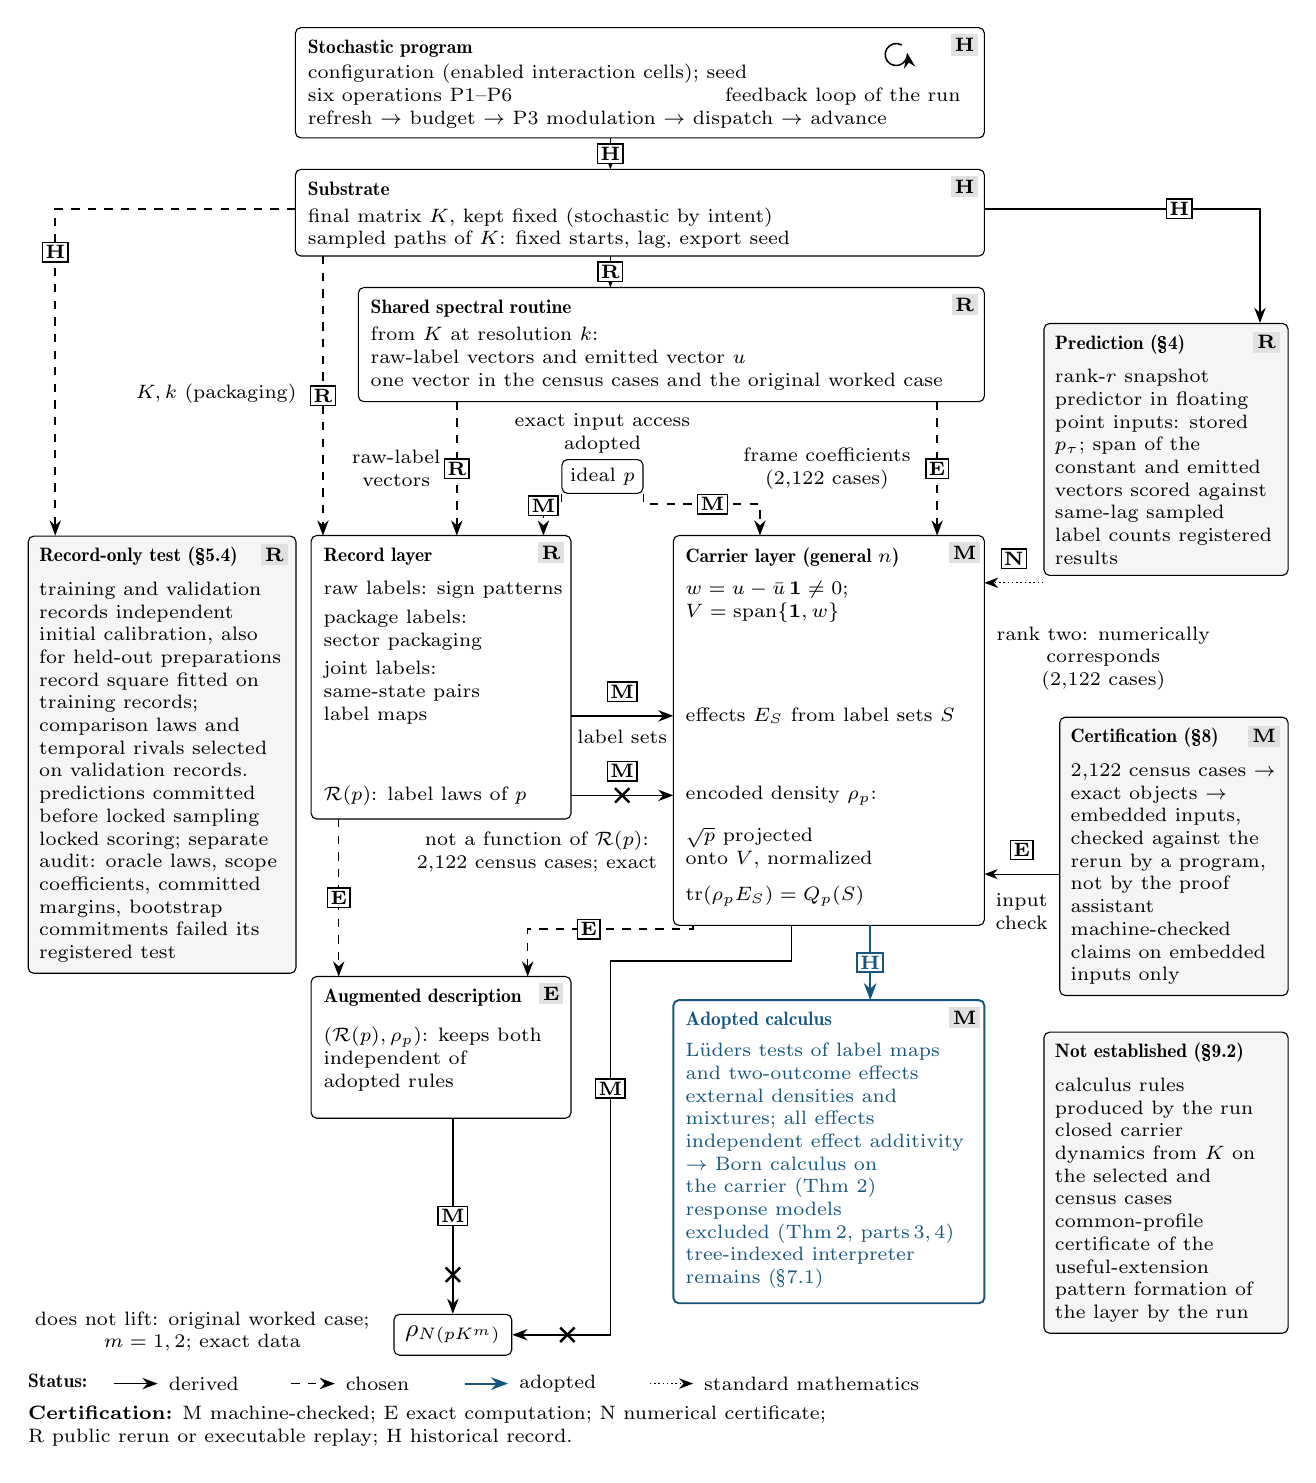
\begin{tikzpicture}[x=1cm,y=1cm,font=\fontsize{7.5}{8.8}\selectfont,
 vtitle/.style={anchor=north west,align=flush left,inner sep=0pt,font=\fontsize{7.5}{8.8}\selectfont\fontseries{b}\selectfont},
 vtext/.style={anchor=north west,align=flush left,inner sep=0pt,font=\fontsize{7.5}{8.2}\selectfont},
 vlabel/.style={align=center,inner sep=0pt,font=\fontsize{7.5}{8.2}\selectfont},
 vbadge/.style={draw,solid,fill=white,inner sep=1.1pt,font=\fontsize{7.5}{8.8}\selectfont\bfseries},
 vcorner/.style={draw=none,fill=black!12,inner sep=1.4pt,font=\fontsize{7.5}{8.8}\selectfont\bfseries},
 vcard/.style={draw,rounded corners=2pt,fill=black!4,anchor=north west,
 align=flush left,inner sep=.14cm,font=\fontsize{7.5}{8.2}\selectfont}]
\draw[band] (3.4,0) rectangle (12.15,-1.4);
\node[vtitle] at (3.55,-0.15) {Stochastic program};
\node[vcorner] at (11.9,-0.22) {H};
\node[vtext,anchor=base west] at (3.55,-0.65)
 {configuration (enabled interaction cells); seed};
\node[vtext,anchor=base west] at (3.55,-0.94) {six operations P1--P6};
\node[vtext,anchor=base west] at (3.55,-1.23)
 {refresh $\to$ budget $\to$ P3 modulation $\to$ dispatch $\to$ advance};
\draw[derived] (11.1,-0.22) arc[start angle=60,end angle=370,radius=.14cm];
\node[vlabel,anchor=base west] at (8.85,-0.94) {feedback loop of the run};
\draw[band] (3.4,-1.8) rectangle (12.15,-2.9);
\node[vtitle] at (3.55,-1.95) {Substrate};
\node[vcorner] at (11.9,-2.02) {H};
\node[vtext] at (3.55,-2.28)
 {final matrix $K$, kept fixed (stochastic by intent)\\
 sampled paths of $K$: fixed starts, lag, export seed};
\draw[band] (4.2,-3.3) rectangle (12.15,-4.75);
\node[vtitle] at (4.35,-3.45) {Shared spectral routine};
\node[vcorner] at (11.9,-3.52) {R};
\node[vtext] at (4.35,-3.8)
 {from $K$ at resolution $k$:\\
 raw-label vectors and emitted vector $u$\\
 one vector in the census cases and the original worked case};
\node[box,inner sep=3pt] (prep) at (7.3,-5.7) {ideal $p$};
\node[vlabel] at (7.3,-5.15) {exact input access\\adopted};
% Record and carrier ports align with the named rows. The record ends just
% below R(p), leaving its X1 scope close to the arrow, clear of augmentation.
\draw[band] (3.6,-6.45) rectangle (6.9,-10.05);
\node[vtitle] at (3.75,-6.6) {Record layer};
\node[vcorner] at (6.65,-6.67) {R};
\node[vtext] at (3.75,-7.02) {raw labels: sign patterns};
\node[vtext] at (3.75,-7.39) {package labels:\\sector packaging};
\node[vtext] at (3.75,-8.04) {joint labels:\\same-state pairs};
\node[vtext,anchor=west] at (3.75,-8.74) {label maps};
\node[vtext,anchor=west] at (3.75,-9.75) {$\mathcal R(p)$: label laws of $p$};
\draw[band] (8.2,-6.45) rectangle (12.15,-11.4);
\node[vtitle] at (8.35,-6.6) {Carrier layer (general $n$)};
\node[vcorner] at (11.9,-6.67) {M};
\node[vtext] at (8.35,-7.02)
 {$w=u-\bar u\,\mathbf1\ne0$;\\$V=\operatorname{span}\{\mathbf1,w\}$};
\node[vtext,anchor=west] at (8.35,-8.74) {effects $E_S$ from label sets $S$};
\node[vtext,anchor=west] at (8.35,-9.75) {encoded density $\rho_p$:};
\node[vtext] at (8.35,-10.15) {$\sqrt p$ projected\\onto $V$, normalized};
\node[vtext] at (8.35,-10.89) {$\operatorname{tr}(\rho_pE_S)=Q_p(S)$};
\draw[band] (3.6,-12.05) rectangle (6.9,-13.85);
\node[vtitle] at (3.75,-12.2) {Augmented description};
\node[vcorner] at (6.65,-12.27) {E};
\node[vtext] at (3.75,-12.69)
 {$(\mathcal R(p),\rho_p)$: keeps both\\independent of\\adopted rules};
\draw[band,draw=accent,line width=.7pt] (8.2,-12.35) rectangle (12.15,-16.2);
\node[vtitle,text=accent] at (8.35,-12.5) {Adopted calculus};
\node[vcorner] at (11.9,-12.57) {M};
\node[vtext,text=accent] at (8.35,-12.89)
 {L\"uders tests of label maps\\and two-outcome effects\\
 external densities and\\mixtures; all effects\\
 independent effect additivity\\
 $\to$ Born calculus on\\the carrier (Thm 2)\\
 response models\\excluded (Thm\,2, parts\,3,\,4)\\
 tree-indexed interpreter\\remains (\S7.1)};
\node[box,inner sep=4pt,font=\fontsize{9}{10.5}\selectfont] (successor) at (5.4,-16.6)
 {$\displaystyle\rho_{N(pK^m)}$};
% Each grey card item has its own bullet and hanging continuation indent.
\node[vcard,text width=3.12cm] (test) at (0,-6.45)
 {{\fontseries{b}\selectfont Record-only test (\S5.4)}\\[4pt]
 \FigCardItem{training and validation records}
 \FigCardItem{independent initial calibration, also for held-out preparations}
 \FigCardItem{record square fitted on training records; comparison laws and temporal rivals selected on validation records.}
 \FigCardItem{predictions committed before locked sampling}
 \FigCardItem{locked scoring; separate audit: oracle laws, scope coefficients, committed margins, bootstrap commitments}
 \FigCardItem{failed its registered test}};
\node[vcorner,anchor=north east] at ([xshift=-3pt,yshift=-3pt]test.north east) {R};
\node[vcard,text width=2.82cm] (prediction) at (12.9,-3.75)
 {{\fontseries{b}\selectfont Prediction (\S4)}\\[4pt]
 \FigCardItem{rank-$r$ snapshot predictor in floating point}
 \FigCardItem{inputs: stored $p_\tau$; span of the constant and emitted vectors}
 \FigCardItem{scored against same-lag sampled label counts}
 \FigCardItem{registered results}};
\node[vcorner,anchor=north east] at ([xshift=-3pt,yshift=-3pt]prediction.north east) {R};
\node[vcard,text width=2.62cm] (certification) at (13.1,-8.75)
 {{\fontseries{b}\selectfont Certification (\S8)}\\[4pt]
 \FigCardItem{\CensusCases{} census cases $\to$ exact objects $\to$ embedded inputs, checked against the rerun by a program, not by the proof assistant}
 \FigCardItem{machine-checked claims on embedded inputs only}};
\node[vcorner,anchor=north east] at ([xshift=-3pt,yshift=-3pt]certification.north east) {M};
\node[vcard,text width=2.82cm] (absent) at (12.9,-12.75)
 {{\fontseries{b}\selectfont Not established (\S9.2)}\\[4pt]
 \FigCardItem{calculus rules produced by the run}
 \FigCardItem{closed carrier dynamics from $K$ on the selected and census cases}
 \FigCardItem{common-profile certificate of the useful-extension pattern}
 \FigCardItem{formation of the layer by the run}};
% Every accepted edge remains; badges are at the midpoints of their paths.
\draw[derived] (7.4,-1.4)--node[vbadge,pos=.5]{H}(7.4,-1.8);
\draw[chosen] (7.4,-2.9)--node[vbadge,pos=.5]{R}(7.4,-3.3);
\draw[chosen] (3.75,-2.9)--node[vbadge,pos=.5]{R}(3.75,-6.45);
\node[vlabel,anchor=east] at (3.42,-4.65) {$K,k$ (packaging)};
\draw[chosen] (5.45,-4.75)--node[vbadge,pos=.5]{R}(5.45,-6.45);
\node[vlabel,anchor=east] at (5.25,-5.6) {raw-label\\vectors};
\draw[chosen] (11.55,-4.75)--node[vbadge,pos=.5]{E}(11.55,-6.45);
\node[vlabel,anchor=east] at (11.22,-5.6)
 {frame coefficients\\(\CensusCases{} cases)};
\draw[chosen,postaction={decorate},decoration={markings,
 mark=at position .5 with {\node[vbadge]{M};}}]
 (prep.south west)--(prep.south west |- 0,-6.05)--(6.55,-6.05)--(6.55,-6.45);
\draw[chosen,postaction={decorate},decoration={markings,
 mark=at position .5 with {\node[vbadge]{M};}}]
 (prep.south east)--(prep.south east |- 0,-6.05)--(9.3,-6.05)--(9.3,-6.45);
\draw[derived] (6.9,-8.74)--node[vbadge,pos=.5,above=5pt]{M}(8.2,-8.74);
\node[vlabel] at (7.55,-9) {label sets};
\draw[crossed] (6.9,-9.75)--node[vbadge,pos=.5,above=5pt]{M}(8.2,-9.75);
\node[vlabel,anchor=north east] at (8,-10.2)
 {not a function of $\mathcal R(p)$:\\ \CensusCases{} census cases; exact};
\draw[chosen] (3.95,-10.05)--node[vbadge,pos=.5]{E}(3.95,-12.05);
\draw[chosen,postaction={decorate},decoration={markings,
 mark=at position .5 with {\node[vbadge]{E};}}]
 (8.45,-11.4)--(8.45,-11.45)--(6.35,-11.45)--(6.35,-12.05);
\draw[adopted] (10.7,-11.4)--node[vbadge,pos=.5]{H}(10.7,-12.35);
\draw[crossed,decoration={markings,
 mark=at position .5 with {\node[vbadge]{M};},
 mark=at position .92 with {
 \draw[line width=.9pt,-](-2.6pt,-2.6pt)--(2.6pt,2.6pt);
 \draw[line width=.9pt,-](-2.6pt,2.6pt)--(2.6pt,-2.6pt);}}]
 (9.7,-11.4)--(9.7,-11.85)--(7.4,-11.85)--(7.4,-16.6)--(successor.east);
\draw[crossed,decoration={markings,mark=at position .8 with {
 \draw[line width=.9pt,-](-2.6pt,-2.6pt)--(2.6pt,2.6pt);
 \draw[line width=.9pt,-](-2.6pt,2.6pt)--(2.6pt,-2.6pt);}}]
 (5.4,-13.85)--node[vbadge,pos=.5]{M}(successor.north);
\node[vlabel,anchor=north east] at (4.35,-16.3)
 {does not lift: original worked case;\\ $m=1,2$; exact data};
\draw[chosen,postaction={decorate},decoration={markings,
 mark=at position .5 with {\node[vbadge]{H};}}]
 (3.4,-2.3)--(.35,-2.3)--(.35,-6.45);
\draw[derived,postaction={decorate},decoration={markings,
 mark=at position .5 with {\node[vbadge]{H};}}]
 (12.15,-2.3)--(15.65,-2.3)--(15.65,-3.75);
\draw[standard] (12.9,-7.05)--node[vbadge,pos=.5,above=5pt]{N}(12.15,-7.05);
\node[vlabel,anchor=north west] at (12.3,-7.6)
 {rank two: numerically\\corresponds\\(\CensusCases{} cases)};
\draw[derived,line width=.4pt] (13.1,-10.75)--node[vbadge,pos=.5,above=5pt]{E}(12.15,-10.75);
\node[vlabel,anchor=north] at (12.625,-10.99) {input\\check};
% Two legend entries; the certification sentence has a deliberate continuation.
\node[vtitle] at (0,-17.1) {Status:};
\draw[derived] (1.1,-17.22)--(1.65,-17.22);\node[anchor=west,inner sep=1pt] at (1.75,-17.22){derived};
\draw[chosen] (3.35,-17.22)--(3.9,-17.22);\node[anchor=west,inner sep=1pt] at (4,-17.22){chosen};
\draw[adopted] (5.55,-17.22)--(6.1,-17.22);\node[anchor=west,inner sep=1pt] at (6.2,-17.22){adopted};
\draw[standard] (7.9,-17.22)--(8.45,-17.22);\node[anchor=west,inner sep=1pt] at (8.55,-17.22){standard mathematics};
\node[vtext] at (0,-17.5)
 {\textbf{Certification:} M machine-checked; E exact computation; N numerical certificate;\\
 R public rerun or executable replay; H historical record.};
\pgfresetboundingbox\path[use as bounding box](0,0)rectangle(16,-18.13);
\end{tikzpicture}}\csgdef{glb@currsize}{}\endgroup}

\newcommand{\FigEncoderCircle}{%
\begingroup%
\normalfont\rmfamily%
\def\EncoderTMin{-1.6259511788473377597974556592752753391671293527443233656649865062978102565197254}%
\def\EncoderTMax{3.8756073400381255552398767818765488226925513353073679400974818157633533341298972}%
\resizebox{\linewidth}{!}{%
\begin{tikzpicture}[x=3.6cm,y=3.6cm,>=Stealth,font=\fontsize{9}{11}\selectfont]
\fill[black!5] (0,0) circle[radius=3.6cm];
\draw[line width=.7pt] (0,0) circle[radius=3.6cm];
\pgfmathsetmacro{\EncoderArcStart}{90-2*atan(\EncoderTMax)}
\pgfmathsetmacro{\EncoderArcEnd}{90-2*atan(\EncoderTMin)}
\draw[accent,line width=2.4pt,line cap=round]
 (\EncoderArcStart:3.6cm) arc[start angle=\EncoderArcStart,end angle=\EncoderArcEnd,radius=3.6cm];
\draw[black!45,->,line width=.4pt] (-1.12,0)--(1.14,0);
\draw[black!45,->,line width=.4pt] (0,-1.1)--(0,1.15);
\node[anchor=west] at (1.17,0) {$x=2t/(1+t^2)$};
\node[anchor=south west] at (.03,1.1) {$z=(1-t^2)/(1+t^2)$};
\node[align=center,text width=3cm] at (-.08,-.38) {densities of the\\adopted calculus};
\node[accent,align=center,text width=2.9cm] (arcname) at (-.38,.45) {image of the encoder};
\draw[accent,->,line width=.5pt] (arcname.west)--(-.91,.41);
\node[anchor=south,align=center,text width=4cm] at (-.1,1.32) {boundary: pure states};
\pgfplotstableread[col sep=comma,row sep=\\]{%
i,bloch_x,bloch_z,joint_label,witness_flag\\
0,0.81434534412073285068862118035767678729921971290954157539986615360235993352462579,0.58038061693072176058592632177804854200490681683035753388256252819819730717030224,2,1\\
1,-0.0092604597630910637034708001851254139697758384277715317975336148340100538439385948,0.99995712102318475933918057293612025574582985570324725260471467322049078848201641,0,0\\
2,0.43471483276677362151295576169349627282043643326318569866520981067858776894208506,0.90056816186924798662762953905921969836533705423110844608529413798523743943947108,2,1\\
3,-0.041419098294384287242645278057231681317633950033391462369136719421447260738268416,0.99914186094692285824695025932147733486768357109029432014637812562308631044055979,0,0\\
4,-0.93517731318713777596293734605854853471900968741589688053797676529889343112556087,-0.35417988776903471427491532191235876489250045650356265737037502383158269718616647,0,0\\
5,-0.99811595679370886423422088797763800962193619590949497172337460969605702859619427,-0.061355821189020848671148729031950111694702668866545679439869502600591179220072450,0,0\\
6,-1.3684643743899113768634112495740057833727813014465198537557687373176468759888010E-17,0.99999999999999999999999999999999990636526280128142336691183999433898083990476745,1,0\\
7,-0.77932702310610237581355651772389193566138422081290868971516217378007426053982903,0.62661742000728049791264729936557451500084781089039960121820276751010005130309326,0,0\\
8,0.99855138444714596959702487851711856890554318079122177399787417946642553950987828,0.053806436591620618282386297104887585931368105820310956524817153463723824542084962,2,0\\
9,0.41547720347975025769183097424493640650561245436813075201095995513531045921855195,0.90960359134550815622373761383457020022851005253935283658220077317534034038627448,2,0\\
10,-0.97971449202429652291301870526441146235513425533983028843598469502688323725810208,0.20039838851042346840806074708390709829261260169794712230287678381891015402864162,0,0\\
11,-1.3684643743899113768634112495740057833727813014465198537558343943143669940505611E-17,0.99999999999999999999999999999999990636526280128142336691183999433898083990476745,1,0\\
12,-0.89246836323363254800511477291084727842946502549109781202212432696496983902242632,-0.45110998728367887424054605868051083947489282015054194598015012708210006329837108,0,0\\
13,-1.3684643743899113768634112495740057833727813014465198537557369179777991259184878E-17,0.99999999999999999999999999999999990636526280128142336691183999433898083990476745,1,0\\
14,0.77071595435970090500242468974546851911650351178177394083942506388535014883138305,0.63717887417538839143358034258219323553349472736789632242546429847187692201088659,2,0\\
15,-0.12142433974393734810758960477499854248124486613700113913139910490999849035530136,0.99260068996437277156362544206897465791078976860861252051177914499178713070392859,0,0\\
16,0.88507317835908412846569697123185513646727661651523299113319488898718653679811474,-0.46545189756767439176192143545550763743799271147043754199217647105269598773891242,2,0\\
17,-0.92889835263376645434516122028654265439736944126458519411779190825693850978854534,-0.37033478161560097461000905557532926648509011126683902662042555830720399891965696,0,0\\
18,0.11840230117224558349527030250274196042628214129266773069043770424609198089111124,0.99296570689884192602546910019801710390657011941578820042667124432635573794039751,2,0\\
19,-0.17839717071618849976171486232888970777765361585965448111620139424803202436403769,0.98395856085531320326510607598993824562902281513728865220015614322475967429614539,1,0\\
20,0.83788542240111033285715431626769787131221086547109116859074053184940593856427983,0.54584614950342272686485660169145194975030414304508822853466043405868085702807832,2,0\\
21,-0.52561968903043969810503549459297492119656521413181801088806957521587138546290488,0.85071966152402042017812888658028219194978506454620452152026631163243361180432528,0,0\\
22,0.45874878635674374436236131279766662139030326691326300934607148810807044338024044,0.88856600824936730447823672298129872185323647036894300128600726243159017688330629,2,0\\
23,0.94863567239171973407623814406090190409952082001898419217890291095634206763956638,-0.31637060714597016669614541391869539224045334741108456261217485357415589938526895,2,0\\
24,-0.37754802165923706839521155076663177986781485980750975843428600992807971732625426,0.92599000606982592719020300841624305471287529317242611837718409470558140530251054,0,0\\
25,-0.61753182579767902290216449018508356455111095103284535646789013401882174682047894,0.78654589448231500435313412547628521824099414339749272197249006108919265810553155,0,0\\
26,-0.93369780723963682807813123512826855456759990473089784321773201646320588510530946,0.35806201244462388408702439304436607448417116740085004226072233672385694519650788,0,0\\
27,-0.85437951146417514035957512576396453850290637373743904446641885423753304988114843,0.51964954574235646098363080802088329874859388783392410469329500584424605651634666,0,0\\
28,-0.83740328025640092319160656778650243181390045670714707810232672818650492593269912,0.54658553421749065877729354914028129173945140648123322952711810416223465989199610,0,0\\
29,-1.3684643743899113768634112495740057833727813014465198537557266088380117997868788E-17,0.99999999999999999999999999999999990636526280128142336691183999433898083990476745,1,0\\
30,-0.73986403792351044402993546322076456329572570027133202492057760989393230368757428,0.67275642352007186129336480338778331849514770319312745839476077696514600550434393,0,0\\
31,0.48383607512664123733189312565468360581460903547918112614700017442157805624090006,-0.87515864413604872795945294699915804207050875687131673026601105563558441421238055,2,0\\
}\points
\pgfplotstablegetrowsof{\points}
\pgfmathtruncatemacro{\lastrow}{\pgfplotsretval-1}
\foreach \r in {0,...,\lastrow}{
 \pgfplotstablegetelem{\r}{bloch_x}\of\points\edef\px{\pgfplotsretval}
 \pgfplotstablegetelem{\r}{bloch_z}\of\points\edef\pz{\pgfplotsretval}
 \pgfplotstablegetelem{\r}{joint_label}\of\points\edef\labelvalue{\pgfplotsretval}
 \pgfplotstablegetelem{\r}{witness_flag}\of\points\edef\witnessvalue{\pgfplotsretval}
 \ifnum\labelvalue=0 \def\shape{*}\else\ifnum\labelvalue=1 \def\shape{square*}\else\def\shape{triangle*}\fi\fi
 \ifnum\witnessvalue=1
  \draw[accent] plot[only marks,mark=\shape,mark size=3.7pt,mark options={fill=accent,draw=accent}] coordinates {(\px,\pz)};
 \else
  \draw[black] plot[only marks,mark=\shape,mark size=2.5pt,mark options={fill=white,draw=black,line width=.6pt}] coordinates {(\px,\pz)};
 \fi
}
\pgfplotstablegetelem{0}{bloch_x}\of\points\edef\zerox{\pgfplotsretval}
\pgfplotstablegetelem{0}{bloch_z}\of\points\edef\zeroz{\pgfplotsretval}
\pgfplotstablegetelem{2}{bloch_x}\of\points\edef\twox{\pgfplotsretval}
\pgfplotstablegetelem{2}{bloch_z}\of\points\edef\twoz{\pgfplotsretval}
\draw[accent,line width=.5pt] (\zerox,\zeroz)--(1.12,.55);
\node[accent,anchor=west] at (1.15,.55) {state $0$};
\draw[accent,line width=.5pt] (\twox,\twoz)--(1.08,.9);
\node[accent,anchor=west] at (1.15,.9) {state $2$};
\node[anchor=north west,align=left,text width=4.1cm] at (1.28,-.16)
 {\StateCount\ point-preparation\\encodings\\[1pt]Joint label:};
\draw plot[only marks,mark=*,mark size=2.5pt,mark options={fill=white}] coordinates {(1.36,-.62)};
\node[anchor=west] at (1.44,-.62) {$a$};
\draw plot[only marks,mark=square*,mark size=2.5pt,mark options={fill=white}] coordinates {(1.36,-.78)};
\node[anchor=west] at (1.44,-.78) {$b$};
\draw plot[only marks,mark=triangle*,mark size=2.5pt,mark options={fill=white}] coordinates {(1.36,-.94)};
\node[anchor=north west,accent,align=left,text width=3.8cm] at (1.29,-1.04)
 {Highlighted census\\witness pair: case \SelectedCaseIndex,\\states $0$ and $2$\\(zero-based indices)};
\node[anchor=west] at (1.44,-.94) {$c$};

\path[use as bounding box] (-1.18,1.52) rectangle (2.9867,-1.50);
\end{tikzpicture}%
}%
\endgroup%
}

\newcommand{\FigThreeDescriptions}{%
\begingroup\normalfont\rmfamily
\csdef{S@9}{%
 \csgdef{tf@size}{9}%
 \csgdef{sf@size}{7}%
 \csgdef{ssf@size}{7}%
}%
\csdef{S@10.95}{%
 \csgdef{tf@size}{10.95}%
 \csgdef{sf@size}{7}%
 \csgdef{ssf@size}{7}%
}%
\csgdef{glb@currsize}{}%
\resizebox{\linewidth}{!}{%
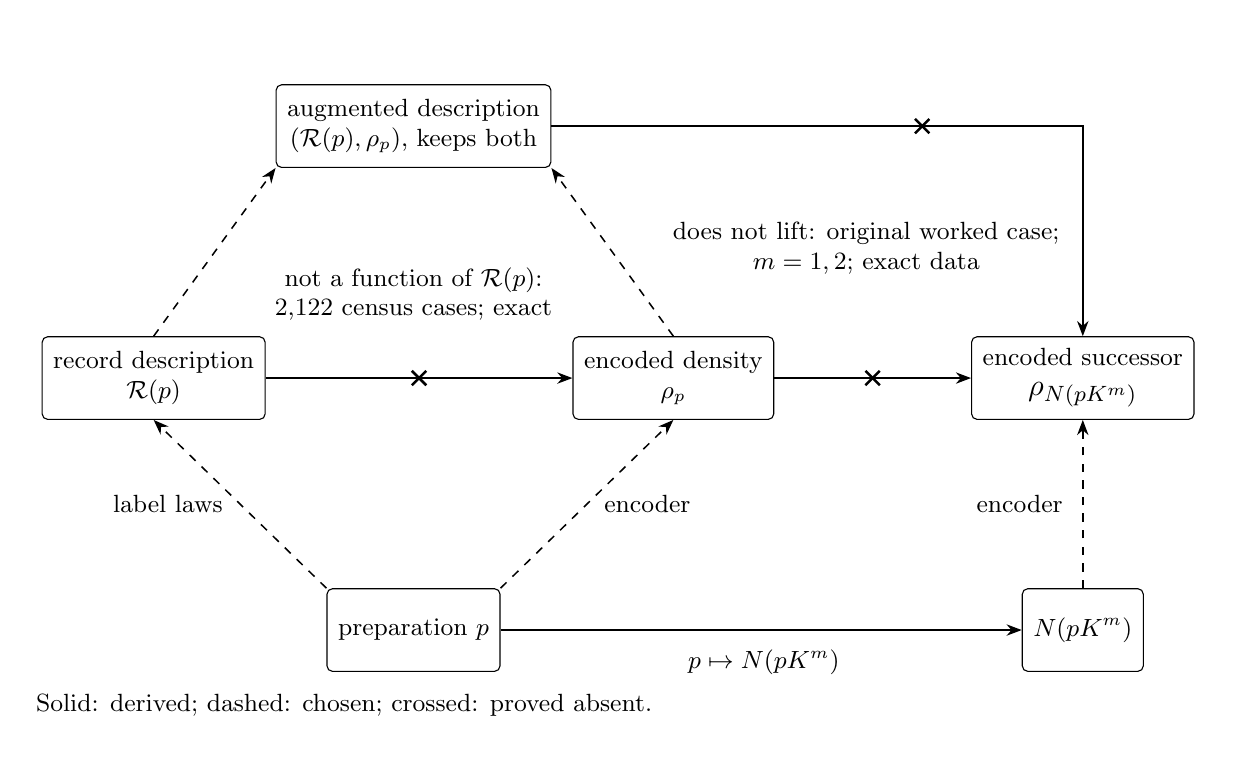
\begin{tikzpicture}[x=1cm,y=1cm,font=\fontsize{9}{10.8}\selectfont,
 desc/.style={box,minimum height=1.05cm,inner sep=4pt},
 scope/.style={align=center,inner sep=0pt}]
\node[desc] (upper) at (4.9,0)
 {augmented description\\$(\mathcal R(p),\rho_p)$, keeps both};
\node[desc] (record) at (1.6,-3.2) {record description\\$\mathcal R(p)$};
\node[desc] (rho) at (8.2,-3.2) {encoded density\\$\rho_p$};
\node[desc] (next) at (13.4,-3.2)
 {encoded successor\\{\fontsize{10.95}{12.5}\selectfont$\displaystyle\rho_{N(pK^m)}$}};
\node[desc] (p) at (4.9,-6.4) {preparation $p$};
\node[desc] (normalized) at (13.4,-6.4) {$N(pK^m)$};
% The four straight chosen edges restore the preparation/description diamond.
\draw[chosen] (p.north west)--node[scope,pos=.5,left=6pt]{label laws}(record.south);
\draw[chosen] (p.north east)--node[scope,pos=.5,right=6pt]{encoder}(rho.south);
\draw[chosen] (record.north)--(upper.south west);
\draw[chosen] (rho.north)--(upper.south east);
\draw[crossed] (record.east)--(rho.west);
\node[scope,anchor=south] at (4.9,-2.48)
 {not a function of $\mathcal R(p)$:\\ \CensusCases{} census cases; exact};
\draw[derived] (p.east)--(normalized.west);
\node[scope,anchor=north] at (9.35,-6.65) {$p\mapsto N(pK^m)$};
\draw[chosen] (normalized.north)--node[scope,pos=.5,left=7pt]{encoder}(next.south);
\draw[crossed] (rho.east)--(next.west);
\draw[crossed] (upper.east)--(13.4,0)--(next.north);
% One shared scope between the two crossed successor inputs.
\node[scope] at (10.65,-1.55)
 {does not lift: original worked case;\\ $m=1,2$; exact data};
\node[anchor=west,inner sep=0pt] at (.1,-7.35)
 {Solid: derived; dashed: chosen; crossed: proved absent.};
\pgfresetboundingbox\path[use as bounding box](0,1.25)rectangle(15,-7.65);
\end{tikzpicture}}\csgdef{glb@currsize}{}\endgroup}
% <<< END FIGURE MACROS

\newcommand{\RepositoryURL}{\url{https://github.com/ioannist/six-birds-born}}
\newcommand{\ReleaseTag}{v1.0}
% Release identity (DOI, date, version), written by paper_set_release.py.
% Generated by scripts/paper_set_release.py.
% The date is the UTC date when this submission was assembled.
\newif\ifpaperhasdoi
\paperhasdoitrue
\newcommand{\paperdoi}{10.5281/zenodo.23261473}
\newcommand{\manuscriptversion}{Preprint v1.0}
\newcommand{\manuscriptdate}{14 October 2026}
\newcommand{\manuscriptyear}{2026}


% The class sets \raggedright in a group that closes before the title
% paragraph ends, so the title would be justified; end it inside the group.
\makeatletter
\patchcmd{\@titleatfontsize}{\endgroup}{\par\endgroup}{}%
  {\PackageError{main}{Could not patch the title alignment}{}}
\makeatother
\title{An Audited Born Calculus on a Pre-Physical Stochastic Substrate}
\author{Ioannis Tsiokos}
\orcid{0009-0009-7659-5964}
\affiliation{Automorph Inc., Wilmington, DE, USA}
\email{ioannis@automorph.io}
\thanks{\textcopyright\ \manuscriptyear\ Automorph Inc. Licensed under CC-BY 4.0
  (Creative Commons Attribution 4.0 International).}
\date{\manuscriptdate\ \textperiodcentered\ \manuscriptversion
  \ifpaperhasdoi\ \textperiodcentered\ DOI:
  \href{https://doi.org/\paperdoi}{\paperdoi}\fi}

\begin{document}
\maketitle
\begin{abstract}
%%% SLOT S0 BEGIN [status: ACCEPTED]
\phantomsection
\label{sec:abstract}
Can a Born-type probability structure arise on a substrate that is only a finite
stochastic process? A stochastic program built from six primitive operations
supplies the final matrix; a specified layered architecture constructs, from
its outputs, a record layer, a two-dimensional real carrier and a quadratic
law, and supports an adopted Born calculus. The six operations alone do not
give this structure, and the square-root encoding and the projection are
construction choices. Our main contribution is the architecture: a directed
acyclic graph whose arrows are each marked as derived, chosen, adopted or
standard mathematics, with the kind of check behind each. On registered
populations, a snapshot predictor whose rank-two case is the law predicts the
substrate's sampled label frequencies with lower aggregate loss than named
competitors, and, in the construction's canonical basis, its cross terms carry its
advantage over the diagonal rule. In each of
\CensusCases{} census cases the encoded state is not a function of the
anonymous initial record description: two point preparations sharing all
three labels differ by at least \RobustGapBound{} in the trace probability of
raw label~\(0\), a statement about exact data, not operational access. This
bound is retrospective: the registered bound \RegisteredRobustGapBound{} fails
in \RegisteredRobustFail{} cases of the full census. On the original worked
case the updates by the final matrix and its square do not lift to the carrier. The measurement rules are adopted:
L\"uders tests, all densities and effects, and additivity; on them the trace
rule is unique, and finite ontic models with additive responses, and measurable
preparation-noncontextual representations preserving the specified mixtures,
are excluded. We do not
claim that the substrate produces the measurement rule, that the layer forms in
the run, or a derivation of quantum theory.
%%% SLOT S0 END
\par\penalty0\relax

\end{abstract}
\tableofcontents

\section{Introduction}
\label{sec:introduction}
%%% SLOT 1a BEGIN [status: ACCEPTED]
\subsection*{The question and the architecture}
\label{sec:question-architecture}
Can a Born-type probability structure arise on a substrate that is nothing but
a finite stochastic process? Hidden-variable theorems constrain what a
stochastic description of quantum statistics can look
like~\cite{Bell1966,Kochen1967}, and several constructions obtain quantum
structure from statistical or stochastic inputs, by selecting the ensemble or
its observables, by postulating a diffusion in physical space, or by
representing a given process in Hilbert
space~\cite{Wetterich2010a,Nelson1966,Barandes2025}. We ask the question from the
other end. We start from a stochastic matrix produced by a program that knows
nothing of quantum theory, and ask what has to be built on top of it, and what
has to be added, before a calculus with the Born rule appears.

The six operations come from \emph{Six Birds}, a mathematical framework for
emergence~\cite{Tsiokos2026Foundations}. In it, a theory of a system is a lens
on the system, a completion rule that packages the lens's stable states into
objects, and an audit; six primitive operations act on these: rewriting the
dynamics (P1), constraining which states are feasible (P2), measuring the
mismatch between two routes of reduction (P3), staging lenses (P4), packaging
(P5) and auditing (P6). The foundations paper argues that, once processes
compose but a system is seen only through a bounded interface, these six
operations arise as unavoidable mechanics of closure, and it describes the
appearance of a new layer as a strict extension of a description. Here the six
operations are implemented as a stochastic program acting on a Markov matrix
(\cref{sec:substrate}). We use the framework's notions of layer and strict
extension; nothing below depends on its general claims, and we do not claim
that all six operations are needed.

Our answer is an architecture (\cref{fig:architecture}). A stochastic program
built from six primitive operations supplies the final matrix; a specified
layered architecture constructs, from its outputs, a record layer, a carrier
and a quadratic law, and supports an adopted Born calculus. Read from the
top of the figure:
\begin{itemize}
\item \emph{The run.} Six operations, coupled through the interaction cells
  that a configuration enables, rewrite and gate a stochastic matrix,
  coarse-grain it by a partition of the states (a lens) and, when a packaging
  cell is enabled, a packaging map on the states, turn audit signals computed through the
  lens into the budget that limits the edits, and modulate how often each
  operation acts. What the operations compute feeds back into what they do;
  this loop is the only cycle in the architecture. The run ends at the final
  matrix \(K\), the substrate.
\item \emph{The record layer.} From \(K\), fixed conventions that we choose
  compute a spectral lens, a sector packaging and their common refinement,
  which label every state, and the \emph{anonymous initial record description} \(\rec(p)\) of a
  preparation \(p\): the laws of its labels at time zero.
\item \emph{The carrier and its law.} From the same \(K\), a spectral routine
  emits a vector; with the constant vector, its centred version spans a
  two-dimensional real carrier. A square-root encoding, an orthogonal
  projection and a normalization, all construction choices, turn each
  preparation into a pure state \(\rho_p\) on the carrier, and the label sets
  into effects whose trace pairing with \(\rho_p\) is a projected-square rule.
\item \emph{The augmented description.} The pair \((\rec(p),\rho_p)\) puts the
  two branches side by side; in every census case it strictly extends \(\rec(p)\).
\item \emph{The adopted calculus.} L\"uders tests, all densities and their
  mixtures, all effects and additivity are adopted, and give the Born calculus
  on the carrier.
\end{itemize}
The run produces \(K\); the record layer and the carrier are derived from it
under conventions and choices that we state; the measurement rules are
adopted. We call the carrier with its encoded states, inherited effects and
law the \emph{constructed layer}. The six operations alone do not give this structure. What the paper
contributes is the architecture itself: which layers there are, how each is
obtained from the ones below, which arrows are derived, chosen, adopted or
standard mathematics, and where certified boundaries separate a layer from a
description below it. The architecture is a directed acyclic graph rather
than a ladder: the record layer and the carrier both come from the final
matrix, and the augmented description combines the two.

The title's terms, and one more, name the parts. The \emph{substrate} is the Markov chain whose
transition matrix is the final matrix of the run; it is \emph{pre-physical}
because no physical interpretation of its states is assumed and it comes with no
apparatus for preparing or measuring it. The \emph{Born calculus} is the
real two-dimensional calculus on the carrier, with all densities as states, all
effects as outcomes and L\"uders tests, in which the trace rule is the only
additive probability rule (\cref{thm:adopted}). It is \emph{audited} in that
every arrow of \cref{fig:architecture} carries the kind of check behind it:
machine-checked proof, exact computation, numerical certificate, executable
replay or historical record. Its \emph{interface
boundaries} are the places, certified with witnesses, where the encoded state
is not a function of the anonymous initial record description, and where the
updates by \(K\) and \(K^2\) do not lift to the carrier on the original worked
case.
%%% SLOT 1a END
\par\penalty0\relax
%%% SLOT FIG1 BEGIN [status: ACCEPTED]
\begin{figure}[tbp]
\centering
\FigArchitecture
\caption{The architecture. The stochastic program, whose feedback loop is the
only cycle, produces the substrate, its final matrix \(K\). Two branches leave
\(K\) and share a spectral routine: the record layer, with the label maps and
the anonymous initial record description \(\rec(p)\) of an ideal preparation
\(p\), and the carrier layer, with the encoded density \(\rho_p\) and the
inherited effects. In the census cases and the original worked case, the raw
labels are the sign pattern of the emitted vector. The branches meet in the
augmented description \((\rec(p),\rho_p)\); the adopted calculus is built on
the carrier. Grey boxes are evidence and supply no input to the construction:
their connectors to the carrier mark the identity of the exact rank-two
formula with the carrier's law (dotted; floating-point correspondence is
certified numerically) and an input check. The bridges listed as
not established are untested, not refuted. Other established results
of \cref{sec:fixture-observations,sec:stochastic-descriptions} are not drawn.
Line styles and badge letters are as in the legend. A framed badge certifies
what its arrow asserts at the scope shown; a grey title badge gives the
strongest certification of the steps inside its box, at its scope. Crossed
arrows are proved absent. Over the ideal preparations, with exact data,
\(\rho_p\) is not a function of \(\rec(p)\) in each of the \CensusCases{}
census cases: two point preparations with the same three labels differ by at
least \RobustGapBound{} in the trace probability of raw label~\(0\); this
bound is retrospective (\cref{app:chronology}). On the original worked case,
whose retained array is used exactly, with no row of \(K\) renormalized (\(N\)
normalizes the propagated preparation), neither \(\rho_p\) nor the augmented
description determines the encoded successor \(\rho_{N(pK^m)}\), for
\(m=1,2\). \Cref{tab:arrow-ledger} lists every arrow.}
\label{fig:architecture}
\end{figure}
%%% SLOT FIG1 END
\par\penalty0\relax

%%% SLOT 1b BEGIN [status: ACCEPTED]
\subsection*{Results and what is assumed}
\label{sec:results-assumptions}
The architecture of \cref{fig:architecture} is the frame of the results; each
of the four components below is one region of it.

\emph{The carrier and its law} (\cref{thm:inherited}). The constant vector and
the centred version of the vector emitted for the final matrix span a two-dimensional real
carrier; encoding a preparation by its square root, projecting and normalizing
gives a pure state; every set of states \(S\), each label set among them,
becomes an inherited effect \(E_S\); and the trace pairing of the two is
exactly a projected-square rule. The single-test statistics of these
effects have an \(n\)-point stochastic model, and when the centred vector takes
at least three distinct values, as in every census case, the family of all
inherited effects \(E_S\), with additivity, does not by itself force
probabilities to come from densities.

\emph{What the law predicts} (\cref{sec:predictive-evidence}). A \emph{snapshot
predictor} projects the entrywise square root of a stored preparation onto a
span that contains the carrier, squares and normalizes; at rank two it is the projected-square rule. On the populations
of the competitor-family and cross-term parts of the corrective evaluation, it
predicts the substrate's sampled label frequencies with lower aggregate loss
than the named competitor rules, and
in the construction's canonical basis, its advantage over the diagonal rule comes
from its cross terms.

\emph{The boundaries} (\cref{sec:interface-boundaries}). The \emph{census}
consists of all \CensusCases{} rank-two cases of a fixed collection of runs
(\cref{sec:cases-provenance}). In each of them the encoded state is not a
function of the anonymous initial record description: two point preparations
with the same labels differ by at least \RobustGapBound{} in trace probability
(\cref{thm:census}). This bound is retrospective: the registered bound
\RegisteredRobustGapBound{} fails in \RegisteredRobustFail{} cases of the full
census. This is a statement about exact data, not about
operational access. On the original worked case, the updates by \(K\) and
\(K^2\) do not induce a dynamics of the encoded state. And a record-only
quadratic law, fitted to label records alone and tested once under a
registered specification, failed its loss criteria; this rejects that law at
its scope, and does not show that the carrier is necessary.

\emph{The extension and what it gives} (\cref{sec:adopted-extension}). The
construction does not produce measurement operations, so we add them: L\"uders
tests of the label maps and of two-outcome effects, all densities and their
mixtures, all effects, and additivity of probabilities over effects as an
independent postulate. These are assumptions of the calculus, not consequences
of the substrate; the carrier and the predictor are constructed before them.
On the adopted calculus the standard results hold, attributed where stated:
program laws, uniqueness of the trace rule, no finite ontic-state
representation with additive responses, and preparation contextuality
(\cref{thm:adopted}).

In the language of Six Birds, these
results instantiate components of a \emph{useful strict extension}, which pairs
a posited object that does not descend with an audited return to an accepted
lower-level answer (\cref{sec:useful-extensions}). A certificate binding the
components to one common problem, and a verdict that the run itself forms the
constructed layer, are not established, and we do not claim a derivation of
quantum theory or of the Born rule from a stochastic model.
%%% SLOT 1b END
\par\penalty0\relax

%%% SLOT 1c BEGIN [status: ACCEPTED]
\subsection*{Relation to prior work, and plan}
\label{sec:prior-work-roadmap}
The uniqueness of the trace rule on the adopted calculus is the real
two-dimensional analogue of the effect-based Gleason-type theorems of Busch and
of Caves et al., contained in Wright and Weigert's analysis of the
rebit~\cite{Busch2003,Caves2004,Wright2021}; Gleason's original theorem
concerns measures on the closed subspaces of a Hilbert space of dimension at
least three~\cite{Gleason1957}. The no-go
statements are Spekkens's six-state argument and an extremality argument also
used by Schmid et al.~\cite{Spekkens2005,Schmid2021}. Barandes represents the
transition maps of stochastic processes entrywise in Hilbert-space
formulas~\cite{Barandes2025}; our carrier is instead a two-dimensional
compression, and on the original worked case the updates by \(K\) and \(K^2\) do
not lift to it.
Wetterich selects observables of a statistical ensemble whose expectation
values define a density matrix, and postulates a rule for sequential
measurements~\cite{Wetterich2010a}; in a phase-space version he modifies the
evolution law so that a coarse-grained evolution closes~\cite{Wetterich2010b}.
Nelson derives the Schr\"odinger equation from a hypothesized diffusion in
physical space~\cite{Nelson1966}. Here the substrate's matrix is produced by a
run and left as it is. Gu et al.\ use quantum models of stochastic processes
for a resource question we do not address~\cite{Gu2012}. A companion paper uses the packaging language of
Six Birds to keep evolution and record formation apart in finite-dimensional
quantum theory, and does not derive the Born rule~\cite{Tsiokos2026QuantumView}.

\Cref{sec:the-substrate-and-the-record-layer} describes the stochastic program
and the record layer, \cref{sec:the-carrier-and-its-inherited-law} the carrier
and its law, \cref{sec:predictive-evidence} what the law predicts, and
\cref{sec:interface-boundaries} the certified boundaries of the constructed
layer. \Cref{sec:the-adopted-calculus} makes the extension and states the
adopted calculus, \cref{sec:stochastic-descriptions-and-strict-extensions}
what stochastic descriptions remain and how the results relate to useful
strict extensions, and \cref{sec:certification} the census and its
certification. \Cref{sec:discussion} discusses what has and has not been
shown.
%%% SLOT 1c END
\par\penalty0\relax

\section{The substrate and the record layer}
\label{sec:the-substrate-and-the-record-layer}
%%% SLOT 2.1 BEGIN [status: ACCEPTED]
\subsection{The substrate: a six-operation stochastic program}
\label{sec:substrate}
Everything in this paper is built on one finite object: a stochastic matrix
\(K\) on a set \(\X=\{0,\dots,n-1\}\) of \(n=\StateCount\) states, acting on
probability vectors by \(p\mapsto pK\). We call the Markov chain with
transition matrix \(K\) the \emph{substrate}. It is pre-physical in this sense:
no physical interpretation of its states is assumed, and the substrate is not
assumed to come with apparatus for preparing or measuring it; the apparatus of
the operational calculus is added in \cref{sec:adopted-extension}. What
distinguishes \(K\) from an arbitrary stochastic matrix is how it is obtained.
It is the final matrix of one run of a stochastic program that edits a matrix
with six primitive operations, the six primitives of Six Birds, listed with
the program's names for them in \cref{tab:six-operations}.

The program's state holds a base stochastic matrix; an effective matrix,
obtained from the base matrix by a gate mask that switches individual
transitions off and renormalizes the rows; the position of a walker on \(\X\);
a budget; and registers in which the operations keep what they last computed.
A run starts from a random matrix with positive entries and performs
\(\RunHorizon\,n\) dispatch steps. At each step one action is drawn at random.
The action with the largest base weight, \(\TrajectoryWeight\), is a walker
move: the walker takes one step of the current effective matrix, and the
matrix is unchanged. The other actions are the operations P1, P2, P4, P5
and P6.

Only the rewrite operation P1 and the gating operation P2 edit the matrix. P1
picks a row with probability proportional to a score and either perturbs it or
blends it toward a scored target row; P2 picks a scored set of transitions and
switches them on or off. A proposal is accepted only if the new effective
matrix is \emph{viable}---every row has entropy at least one tenth of \(\ln
n\), no state returns to itself with probability above \(1-\tfrac{1}{n}\), and
the graph of positive transitions, with directions ignored, is connected---and
only if the budget covers its cost, a thresholded relative entropy of the new
effective matrix against the old (negligible entries are ignored, a penalty
per unit of new probability applies where an old entry was negligible, and P2
carries a multiplier set by the enabled cells; \cref{app:program-details}).

The lens operation P4 refreshes a \emph{lens}: a partition of \(\X\) computed
from the current matrix and chosen among enabled candidates, one of which is
the spectral sign partition of \cref{sec:record-layer}. The packaging operation
P5, when a packaging cell is enabled, refreshes a \emph{packaging} of that
partition, one candidate being the sector packaging of \cref{sec:record-layer}.
Neither edits the matrix. From the lens the program also computes, on fixed
schedules, an \emph{audit}, a summary of the lagged matrix coarse-grained
through the lens (such as its distance from a rank-one matrix), and a
\emph{route mismatch}: for each block of the lens, how much the lagged
transition rows of its states, coarse-grained to blocks, disagree with their
block average. The audit operation P6 sets, from audit signals, the rate and
the cap at which the budget is replenished at every step, and a drawn P6 adds
ten times the base rate, up to the base cap. The modulation operation P3 is
never drawn. It rescales the dispatch weights using the route mismatch and
other cached signals, and one of its cells adapts the lag at which the route
mismatch and the audit are computed. A fixed cyclic schedule, the protocol
phase, also boosts P2, P1 and P6 in turn.

The operations are coupled through a \(6\times 6\) array of interaction cells,
indexed by an acting operation and an informing one (written actor
\(\leftarrow\) informant). In an action cell the informant's current output
parameterizes what the actor does: one cell biases P2 toward switching off
transitions between the current lens's blocks and against switching them back
on; another lets P4 use sign patterns of spectral vectors as its lens. The
informant-only cells record that an edit by P1 or P2 changes the matrix that
every later refresh reads; they mediate no edits. A \emph{configuration} is a
set of enabled cells together with its numerical and cadence parameters; the
cases of \cref{sec:certification} come from seven families of configurations
(\cref{app:program-details}).

The run therefore contains a feedback loop. Depending on the enabled cells,
the lens and the packaging are recomputed from the matrix on fixed schedules
and when P4 or P5 is drawn, the audit on its own schedule or after a change of
lens, and the operations that edit the matrix read all three. With the cell P1\,\(\leftarrow\)\,P4 enabled,
for example, P1's choice of row is biased toward states whose outgoing
transitions cross the boundaries of the current lens's blocks; the lens is
recomputed from the edited matrix at its next refresh, which may change the
blocks and with them the scores that guide the next edits. This loop is the
only cycle in the architecture, and \cref{fig:architecture} draws it inside
its top node.

The configuration and the seed are inputs chosen for each run, and the
initial matrix is generated from that seed; the final effective matrix \(K\)
is the run's output, and after the run
it is kept fixed. Every later construction is a function of \(K\) and of
separately supplied inputs: preparations, sampling seeds and lags,
construction choices, and, from \cref{sec:adopted-extension} on, adopted
rules. Sampling uses the double-precision rows of \(K\), as the run did; exact
constructions read the same stored entries as exact rationals and never
renormalize a row (\cref{sec:no-lift}). In particular, the record layer below
is recomputed from \(K\) by fixed conventions; it is not read from the lens and
packaging the run last held. We do not claim that all six operations are
needed for what follows.
%%% SLOT 2.1 END
\par\penalty0\relax
%%% SLOT TAB1 BEGIN [status: ACCEPTED]
\begin{table}[tbp]
\caption{The six primitive operations of the stochastic program and the
walker's move: what each acts on, whether it edits the matrix, and its base
dispatch weight in the runs that produced the cases of this paper. The protocol
phase and P3 modulate these weights during a run; edits by P1 and P2 are
accepted only if the edited matrix is viable and the budget covers their cost
(\cref{sec:substrate}).}
\label{tab:six-operations}
\centering\small
\setlength{\tabcolsep}{4pt}
\begin{tabularx}{\linewidth}{@{}>{\raggedright\arraybackslash}p{0.9cm}>{\raggedright\arraybackslash}p{1.9cm}>{\raggedright\arraybackslash}X>{\raggedright\arraybackslash}p{2.0cm}>{\raggedright\arraybackslash}p{2.3cm}@{}}
\toprule
 & Name & What it acts on & Edits the matrix? & Base dispatch weight \\
\midrule
P1 & Rewrite & A scored row of the base matrix (perturbation, or blending toward a scored target) & Yes & \RewriteWeight{} \\
P2 & Gating & A scored set of transitions in the gate mask & Yes, through the gate mask & \GateWeight{} \\
P3 & Modulation & The dispatch weights, from cached signals such as the route mismatch; with one of its cells, the lag of those signals & No & none; modulates the others \\
P4 & Lens & A partition of the states, chosen among enabled candidates & No & \LensWeight{} \\
P5 & Packaging & A packaging of the lens, when a packaging cell is enabled & No & \PackagingWeight{} \\
P6 & Audit & The budget's replenishment rate and cap, set from audit signals; a boost when drawn & No & \BudgetWeight{} \\
-- & Walker move & The walker's position, moved by the current effective matrix & No & \TrajectoryWeight{} \\
\bottomrule
\end{tabularx}
\end{table}
%%% SLOT TAB1 END
\par\penalty0\relax

%%% SLOT 2.2 BEGIN [status: ACCEPTED]
\subsection{The record layer}
\label{sec:record-layer}
This is the record layer of \cref{fig:architecture}, one of the two branches
that leave the final matrix; the carrier layer of
\cref{sec:the-carrier-and-its-inherited-law} is the other. After the run, three label maps are computed from \(K\) by conventions that
are fixed in advance and are the same for every case. They do not depend on
which lens and packaging the run itself used, and they are not read from the
run's registers.

\paragraph{Spectral lens.} The export routine begins by estimating a stationary
vector \(\pi\) by iterating \(p\mapsto pK\) from the uniform vector. It then
runs the program's spectral routine, the one P4 uses for its spectral sign
partition, which has two branches. If every component of \(\pi\) exceeds a small fixed
threshold, it diagonalizes a symmetrized form of \(K\); otherwise it runs a
deflated power iteration of the row action \(v\mapsto vK\) from a fixed
deterministic start vector, removing the stationary direction at each step
(\cref{app:record-details}). The \CensusCases{} census cases (every rank-two case of the fixed
collection of \cref{sec:cases-provenance}, without performance filtering) and
the original worked case all take the second branch. The \emph{resolution} \(k\) is the
requested number of raw labels. With \(k=2\) the routine returns one vector
\(u\), the \emph{emitted vector}, and the raw label of a state is the sign of
its component of \(u\). No eigenvalues are computed or ordered in this branch,
and we do not call \(u\) an eigenvector; nothing below needs it to be one. In
these cases a single vector both defines the labels and is returned for later
use; in the other branch, which none of them takes, the two roles are filled
by different vectors (\cref{app:record-details}). At higher resolutions the
routine returns several vectors, and the predictor of
\cref{sec:predictive-evidence} uses all of them.

\paragraph{Sector packaging.} The package map refines and then merges the raw
labels using \(K\). Each raw block with more than \(\lceil\tfrac{2n}{5}\rceil\)
states (and at least four) is split in two by applying the same spectral
routine to the restriction of \(K\) to that block, with each row
renormalized (a row with negligible mass inside the block is replaced by the
uniform row on the block), and with a fixed half-split of the block's ordered
states when that bisection leaves one side empty. Each block left
with a single state is then merged into the block it is most strongly
connected to, as measured by \(\sum_{j}(K_{ij}+K_{ji})\) over the block's
states \(j\). The complete procedure is given in \cref{app:record-details}.

\paragraph{Joint labels.} The joint map labels each state by the pair (raw
label, package label) that it carries, the common refinement of the two maps;
its labels are the pairs that occur, not all pairs.

Write \(f\) for any of the three label maps \(\fraw,\fpkg,\fjnt\), and \(f_*p\)
for the label law of a probability vector \(p\) in the set \(\simplex\) of
probability vectors on \(\X\),
\(f_*p(j)=\sum_{i:\,f(i)=j}p_i\). The \emph{record description} of a
preparation \(p\) is
\[
  \rec(p)=\bigl(\fraw{}_*p,\ \fpkg{}_*p,\ \fjnt{}_*p\bigr),
\]
together with fixed fields that do not depend on \(p\): the case, an
anonymous preparation label, time zero, and empty lists of acquired records,
tests and outcomes (the complete list is in \cref{app:record-details}). We
call it the \emph{anonymous initial record description}:
anonymous because nothing in it names \(p\), initial because it describes
\(p\) before anything is done; for short we also call it the record
description. Since the joint label determines the raw and the
package label, \(\rec(p)\) carries exactly the information of the joint label
law. It is the lower description against which \cref{sec:interface-boundaries}
measures the constructed layer, and four other things should not be confused
with it: the label maps themselves; the ideal label laws \(f_*p\); sampled
label records, which are counts along sampled paths; and the program's literal
output rows, which also list the states that carry each label. A description
that includes \(p\) itself determines everything constructed from \(p\)
(\cref{sec:strict-extension}).

The record layer also supplies the data against which the constructed law is
tested in \cref{sec:predictive-evidence}. Each case has a lag \(\tau\), the
run's final adaptive lag when one exists and otherwise a value set by the
spectral gap of \(K\) (\cref{app:record-details}). The starting distribution
\(p_0\) is uniform on the states \(i<\Trajectories\); propagating it
deterministically, in double precision, for \(\tau\) steps gives the stored
preparation \(p_\tau=p_0K^\tau\) that the predictor receives. Separately,
\Trajectories{} paths are sampled, one from each of those starting states, with
seeds derived from the run's seed, and run for \(\tau\) steps; the counts of
each raw and package label among their final states, divided by the number of
paths, give the empirical endpoint frequencies used in the registered scoring.
Here and below, \emph{registered} means specified prospectively, in a signed
specification, for the stated evaluation, with any amendment disclosed.
Joint endpoint labels can be reconstructed from the same paths but are not a
registered scoring input. Sampling and propagation happen after the run and do
not feed back into it.

The carrier of \cref{sec:carrier-rule} is built from the same emitted vector.
Its stored double-precision components are read as exact rationals and centred
exactly, giving \(w=u-\bar u\,\ones\) with \(\bar u\) the mean of the
components of \(u\). Four construction choices follow: the carrier is the
plane \(V=\operatorname{span}\{\ones,w\}\subset\mathbb{R}^n\); a preparation
\(p\) is encoded by its entrywise square root \(\sqrt p\); that vector is
projected orthogonally onto \(V\); and the result is normalized.
\Cref{fig:architecture} shows these steps as the carrier layer.

We call a final matrix together with its emitted vector or vector family, its
three label maps,
its lag and its starting distribution a \emph{case}; \(\delta_i\) denotes the
point mass at state \(i\). Two cases are worked in detail: the \emph{selected worked case}, case
\SelectedCaseIndex{} of the census of \cref{sec:certification}, and the \emph{original
worked case}, a single case outside the census, fixed earlier for the analyses
of \cref{sec:no-lift,sec:fixture-observations}.

Two facts about this layer are checked by executable replay of the public
source rather than assumed (\cref{app:record-details}), for the \CensusCases{}
census cases and the original worked case: recomputing the three maps from the retained
matrices reproduces the retained maps exactly; and the raw labels are the
signs of the emitted vector, whose centred version, together with the
constant vector, spans the carrier. Neither statement is
made for cases with several emitted vectors.
%%% SLOT 2.2 END
\par\penalty0\relax

\section{The carrier and its inherited law}
\label{sec:the-carrier-and-its-inherited-law}
%%% SLOT 3.1 BEGIN [status: ACCEPTED]
\subsection{The carrier and the projected-square rule}
\label{sec:carrier-rule}
This section builds the carrier layer of \cref{fig:architecture} from the
emitted vector and states what follows from the construction. The input from
the substrate is small: the label maps of \cref{sec:record-layer} and one real
vector.

\begin{definition}[Substrate data]\label{def:substrate-data}
A finite set \(\X=\{0,\dots,n-1\}\) with \(n\ge 2\), label maps
\(f\colon\X\to L_f\), and a real vector \(u\in\mathbb{R}^n\) whose exact
centring \(w=u-\bar u\,\ones\) is nonzero. Write \(s=w^{\mathsf T}w\). In the
cases of this paper \(n=\StateCount\), \(u\) is the emitted vector of \(K\), and
the label maps are \(\fraw,\fpkg,\fjnt\).
\end{definition}

\begin{definition}[Carrier and encoder]\label{def:carrier}
The \emph{carrier} is the plane \(V=\operatorname{span}\{\ones,w\}\subset
\mathbb{R}^n\), with orthonormal basis \(e_0=\ones/\sqrt n\), \(e_1=w/\sqrt s\).
Let \(B=[e_0\ e_1]\) be the \(n\times 2\) isometry and \(P=BB^{\mathsf T}\) the
orthogonal projector onto \(V\). For \(p\in\simplex\) let \(\sqrt p\) be the
entrywise square root, \(\psi_p=B^{\mathsf T}\sqrt p/\lVert B^{\mathsf T}\sqrt
p\rVert\in\mathbb{R}^2\), and \(\rho_p=\psi_p\psi_p^{\mathsf T}\). The map
\(p\mapsto\rho_p\) is the \emph{encoder}.
\end{definition}

\begin{definition}[Inherited effects; states and effects]\label{def:effects}
For \(S\subseteq\X\) let \(\Pi_S\) be the diagonal indicator of \(S\) and
\(E_S=B^{\mathsf T}\Pi_S B\). For a label map \(f\) and a label \(j\), write
\(E_{f,j}=E_{f^{-1}(j)}\). Let \(\States\) be the set of real \(2\times 2\)
densities (positive semidefinite, trace one) and \(\Effects\) the set of real
symmetric \(2\times 2\) matrices \(E\) with \(0\le E\le I\).
\end{definition}

The \emph{projected-square rule} assigns to a preparation \(p\) and a set
\(S\subseteq\X\) the number
\[
  Q_p(S)=\frac{\lVert\Pi_S P\sqrt p\rVert^2}{\lVert P\sqrt p\rVert^2}.
\]
It squares the projection of the square-root vector onto the carrier and
reads off the mass on \(S\). Four steps of this construction are choices, not
consequences of anything the run does: taking the span of the constant and the
emitted vector as the carrier; encoding a probability vector by its square
root, the representation in which statistical distance becomes an
angle~\cite{Wootters1981,Braunstein1994}; projecting orthogonally; and
normalizing. Given an ideal preparation \(p\), which
is a separate input, the remaining quantities are computed from these choices
and the substrate data. Hypotheses below carry tags: [D] derived from the substrate's
data, [C] a construction choice, [A] adopted, [S] standard mathematics.

\begin{definition}[Strict refinement]\label{def:strict-refinement}
Let \(\mathcal D\) be a map on \(\simplex\), a \emph{description} of
preparations. The augmented description \((\mathcal D,\rho)\colon
p\mapsto(\mathcal D(p),\rho_p)\) \emph{strictly refines} \(\mathcal D\) if
there are \(p,p'\) with \(\mathcal D(p)=\mathcal D(p')\) and
\(\rho_p\ne\rho_{p'}\); equivalently, \(\rho\) does not factor through
\(\mathcal D\).
\end{definition}

The augmented description keeps \(\mathcal D\); nothing is said about \(\rho\)
alone determining \(\mathcal D\).

\begin{theorem}[The inherited construction and its limits]\label{thm:inherited}
\emph{[C: the span \(V\), the orthogonal projection, the square-root encoding
and the normalization. D: \(w\), computed from the emitted vector, and the
label maps, computed from \(K\) under the fixed export conventions.]} Let the data be as in \cref{def:substrate-data,def:carrier,def:effects}.
\begin{enumerate}
\item \emph{Carrier and trace identity.} \(\rho_p\) is a pure density for every
  \(p\in\simplex\). For every label map \(f\) the \(E_{f,j}\) are effects that
  sum to \(I\), and they are coarse-grainings of the single family
  \(\{E_{\{i\}}\}_{i\in\X}\). For every \(p\) and \(S\),
  \(Q_p(S)=\tr(\rho_p E_S)\).
\item \emph{Image of the encoder.} \(\psi_p\propto(1,t_p)\) with
  \(t_p=\sqrt{\tfrac{n}{s}}\,\sum_i w_i\sqrt{p_i}\big/\sum_i\sqrt{p_i}\), and as \(p\)
  ranges over \(\simplex\), \(t_p\) ranges exactly over
  \([\sqrt{\tfrac{n}{s}}\,\min_i w_i,\ \sqrt{\tfrac{n}{s}}\,\max_i w_i]\). The image of the
  encoder is an arc of pure states, never the whole state space, and the
  encoder is not affine.
\item \emph{Single-test statistics have an \(n\)-point model.} For every
  \(R\in\States\), \(\kappa_R(i)=\tr(RE_{\{i\}})\) is a probability vector on
  \(\X\), and \(\tr(RE_{f,j})=\sum_{i:\,f(i)=j}\kappa_R(i)\) for every label
  map. The inherited positive-operator-valued measures are jointly
  measurable.
\item \emph{The inherited effects do not force representation by a positive
  density.} There is a real symmetric \(R\) of trace one that is not positive
  semidefinite such that \(0<\tr(RE_S)<1\) for every nonempty proper
  \(S\subset\X\), and \(S\mapsto\tr(RE_S)\) is additive over disjoint unions
  with value \(1\) at \(\X\). If \(w\) takes at least three distinct values, no
  density gives the same values on the \(E_S\).
\item \emph{Strict refinement of record descriptions.} If two states
  \(i\ne j\) carry the same label under every label map and \(w_i\ne w_j\), then
  \(\rec(\delta_i)=\rec(\delta_j)\) and \(\rho_{\delta_i}\ne\rho_{\delta_j}\):
  the augmented description \((\rec,\rho)\) strictly refines \(\rec\). If
  instead the description contains \(p\) itself, \(\rho_p\) is a function of it.
\end{enumerate}
\end{theorem}

That is: the construction turns a probability vector into a pure state on a
two-dimensional real carrier, and label sets into effects whose trace pairing
is exactly the projected-square rule. The single-test statistics of these
effects are those of drawing a state from \(\kappa_R\) and reading its labels;
no sequential instrument representation, and no responses for effects outside
the inherited family, are asserted. When \(w\) takes at least three distinct
values, the effects alone admit additive assignments that no density
reproduces. When two states with the same labels have different values of
\(w\), the encoded state separates preparations that the record description
identifies; \cref{sec:strict-extension} shows that this holds in each of the
\CensusCases{} census cases. \Cref{thm:inherited} uses no adopted rule. It is a
statement about ideal preparations \(p\in\simplex\) and asserts nothing about
operational access to them. Parts~1 and~2 are proved in
\cref{sec:trace-encoder-image}, parts~3 and~4 in \cref{sec:single-tests}, and
part~5 in \cref{sec:strict-extension}, where it is applied to the
\CensusCases{} census cases.
%%% SLOT 3.1 END
\par\penalty0\relax

%%% SLOT 3.2 BEGIN [status: ACCEPTED]
\subsection{The trace identity and the image of the encoder}
\label{sec:trace-encoder-image}
We prove parts~1 and~2 of \cref{thm:inherited}.

\begin{proposition}[Carrier and trace identity]\label{prop:trace}
Let the data be as in \cref{def:substrate-data,def:carrier,def:effects}.
\begin{enumerate}
\item[(a)] \(B^{\mathsf T}\sqrt p\ne 0\) and \(\rho_p\in\States\) is pure for
  every \(p\in\simplex\).
\item[(b)] \(E_S\in\Effects\), \(E_\emptyset=0\), \(E_\X=I\), and
  \(E_{S\cup T}=E_S+E_T\) for disjoint \(S,T\). Hence for each label map \(f\)
  the family \(\{E_{f,j}\}_j\) is a positive-operator-valued measure and a
  coarse-graining of \(\{E_{\{i\}}\}_{i\in\X}\).
\item[(c)] \(Q_p(S)=\tr(\rho_pE_S)\) for every \(p\) and \(S\).
\end{enumerate}
\end{proposition}

\begin{proof}
(a) The \(e_0\)-coordinate of \(B^{\mathsf T}\sqrt p\) is
\(\sum_i\sqrt{p_i}/\sqrt n>0\). (b) The \(\Pi_S\) are orthogonal projectors that
add over disjoint sets and sum to the identity, and \(B^{\mathsf T}B=I\); so
\(0\le B^{\mathsf T}\Pi_SB\le B^{\mathsf T}B=I\), with the additivity inherited
from the \(\Pi_S\). (c) \(P\sqrt p=BB^{\mathsf T}\sqrt p\), so
\(\lVert\Pi_SP\sqrt p\rVert^2=(B^{\mathsf T}\sqrt p)^{\mathsf T}E_S(B^{\mathsf
T}\sqrt p)\) and \(\lVert P\sqrt p\rVert^2=\lVert B^{\mathsf T}\sqrt
p\rVert^2\); divide.
\end{proof}

The family \(\{E_{\{i\}}\}\) is the compression to \(V\) of the coordinate
projection-valued measure on \(\mathbb{R}^n\), a standard way of obtaining a
positive-operator-valued measure on a subspace. The identity in~(c) is
between two constructed quantities. It does not say that the label
probabilities of the chain, \(f_*p\), are trace pairings: \(Q_p(S)\) and
\(p(S)=\sum_{i\in S}p_i\) differ in general, and whether \(Q_p\) predicts
anything about the chain is the question of \cref{sec:predictive-evidence}.

\begin{proposition}[Image of the encoder]\label{prop:image}
Write \(\psi_p\propto(1,t_p)\) with
\(t_p=\sqrt{\tfrac{n}{s}}\,\sum_iw_i\sqrt{p_i}\big/\sum_i\sqrt{p_i}\).
\begin{enumerate}
\item[(a)] \(\{t_p:p\in\simplex\}=[\sqrt{\tfrac{n}{s}}\,\min_iw_i,\ \sqrt{\tfrac{n}{s}}\,\max_iw_i]\).
\item[(b)] The image of the encoder is the set of pure states
  \(\psi\psi^{\mathsf T}\) with \(\psi\propto(1,t)\) and \(t\) in that interval: a
  closed arc that contains the encoding \((1,0)\) of the uniform preparation in
  its interior and never contains the orthogonal pure state \((0,1)\).
\item[(c)] If \(\rho_p\ne\rho_{p'}\) and \(0<\theta<1\), then
  \(\rho_{\theta p+(1-\theta)p'}\ne\theta\rho_p+(1-\theta)\rho_{p'}\).
\end{enumerate}
\end{proposition}

\begin{proof}
(a) \(t_p/\sqrt{\tfrac{n}{s}}\) is the average of the \(w_i\) with weights
\(a_i/\sum_ja_j\), \(a_i=\sqrt{p_i}\). Every weight vector in the simplex
arises (take \(p_i\propto a_i^2\)), and such averages fill \([\min w,\max w]\).
(b) Because \(w\) is centred and nonzero, \(\min_iw_i<0<\max_iw_i\); the uniform
preparation gives \(t=0\), and no finite \(t\) gives \((0,1)\). (c) The left
side has rank one; the right side is a proper mixture of two distinct pure
states and has rank two.
\end{proof}

So the encoder does not map the simplex onto the state space of the adopted
calculus, and it does not respect mixing: mixing two preparations of the chain
and mixing their encoded states are different operations.
\Cref{fig:encoder-circle} shows the arc for the selected worked case, with the
encodings of the \StateCount{} point preparations.
%%% SLOT 3.2 END
\par\penalty0\relax
%%% SLOT FIG2 BEGIN [status: ACCEPTED]
\begin{figure}[tbp]
\centering
\FigEncoderCircle
\caption{The image of the encoder for the selected worked case, drawn on the
disk of real \(2\times2\) densities. A pure state \(\psi\propto(1,t)\) is
plotted at \(\bigl(\tfrac{2t}{1+t^2},\tfrac{1-t^2}{1+t^2}\bigr)\); the thick arc
is the image of the encoder, \(t\in[\sqrt{\tfrac{n}{s}}\min_iw_i,\
\sqrt{\tfrac{n}{s}}\max_iw_i]\) (\cref{prop:image}). The markers are the
encodings of the \StateCount{} point preparations only, shaped by joint label.
Markers of the same shape at different positions are preparations with the
same record description and different encoded states, which is what strict
refinement means (\cref{sec:strict-extension}); the highlighted pair is this
case's lexicographic pair, states \(0\) and \(2\).}
\label{fig:encoder-circle}
\end{figure}
%%% SLOT FIG2 END
\par\penalty0\relax

%%% SLOT 3.3 BEGIN [status: ACCEPTED]
\subsection{Single tests, and what the inherited effects do not force}
\label{sec:single-tests}
We prove parts~3 and~4 of \cref{thm:inherited}. Both concern the inherited
effects alone, before anything is added to the construction.

\begin{proposition}[Single-test statistics have an \(n\)-point model]\label{prop:n-point}
For \(R\in\States\) put \(\kappa_R(i)=\tr(RE_{\{i\}})\). Then
\(\kappa_R\in\simplex\) and \(\tr(RE_S)=\sum_{i\in S}\kappa_R(i)\) for every
\(S\subseteq\X\). In particular \(\tr(RE_{f,j})\) is the probability that a
point drawn from \(\kappa_R\) carries label \(j\), for every label map \(f\)
simultaneously. For \(R=\rho_p\), \(\kappa_R(i)=Q_p(\{i\})\).
\end{proposition}

\begin{proof}
By \cref{prop:trace}, \(E_{\{i\}}\ge 0\), \(\sum_iE_{\{i\}}=I\) and
\(E_S=\sum_{i\in S}E_{\{i\}}\).
\end{proof}

The inherited positive-operator-valued measures are coarse-grainings of one
parent, so they are jointly measurable; this is a statement about the measures,
not about any particular instrument that realizes them. The proposition gives
a stochastic model of event-labelled single-test statistics: draw a state from
\(\kappa_R\) and read its labels. It gives no model of sequences of tests and
no response model for effects outside the inherited family.

The next result asks whether the inherited effects, with additivity of
probabilities over them, already force probabilities to come from densities.
When \(w\) takes at least three distinct values, they do not.

\begin{proposition}[Failure of density representability on the inherited effects]\label{prop:no-force}
For \(\varepsilon>0\) let \(R_\varepsilon=\operatorname{diag}(1+\varepsilon,
-\varepsilon)\) in the basis \((e_0,e_1)\). For every sufficiently small
\(\varepsilon\):
\begin{enumerate}
\item[(a)] \(\tr R_\varepsilon=1\), and \(R_\varepsilon\) is not positive
  semidefinite;
\item[(b)] \(0<\tr(R_\varepsilon E_S)<1\) for every nonempty proper
  \(S\subset\X\);
\item[(c)] \(S\mapsto\tr(R_\varepsilon E_S)\) is additive over disjoint unions,
  with value \(0\) at \(\emptyset\) and \(1\) at \(\X\), and respects every linear
  relation among the \(E_S\).
\end{enumerate}
If moreover \(w\) takes at least three distinct values, then
\begin{enumerate}
\item[(d)] no density \(R\) satisfies \(\tr(RE_{\{i\}})=\tr(R_\varepsilon
  E_{\{i\}})\) for all \(i\).
\end{enumerate}
\end{proposition}

\begin{proof}
(a) is immediate. (b) The diagonal entries of \(E_S\) are
\((E_S)_{0,0}=\tfrac{|S|}{n}\) and
\((E_S)_{1,1}=\tfrac{1}{s}\sum_{i\in S}w_i^2\in[0,1]\), so
\[
  \tr(R_\varepsilon E_S)=\frac{|S|}{n}+\varepsilon\Bigl(\frac{|S|}{n}
  -\frac{1}{s}\sum_{i\in S}w_i^2\Bigr).
\]
For nonempty proper \(S\) the leading term lies strictly
between \(0\) and \(1\), and there are finitely many \(S\), so the sum does too
for all \(\varepsilon\) below a positive bound. (c) The trace is linear.
(d) \(E_{\{i\}}=b_ib_i^{\mathsf T}\) with \(b_i=\bigl(\tfrac{1}{\sqrt n},\tfrac{w_i}{\sqrt s}\bigr)\).
After fixed nonzero rescalings of the coordinates, the three independent
entries of \(b_ib_i^{\mathsf T}\) are \((1,w_i,w_i^2)\); three distinct values of \(w_i\) give three
linearly independent such vectors (a Vandermonde determinant), so the
\(E_{\{i\}}\) span the real symmetric \(2\times 2\) matrices. A density agreeing
with \(R_\varepsilon\) on a spanning set equals \(R_\varepsilon\), which is not
positive semidefinite.
\end{proof}

Parts (a)--(c) give an indefinite trace assignment: a trace pairing with a
matrix that is not positive semidefinite, additive and with values strictly
inside \((0,1)\). By itself this does not exclude densities, because without a
spanning family a density may give the same values (for \(n=2\) and
\(w=(1,-1)\), \(R_\varepsilon\) and \(\tfrac{1}{2}I\) agree on every inherited
effect). The hypothesis on \(w\) is what makes the one-point effects separate
symmetric matrices, and only then does (d) follow. In every census case the
hypothesis holds: the lexicographic pair of \cref{sec:strict-extension} has
equal raw labels, so two distinct values of \(u\) of the same sign, and a
state with the other raw label supplies a value of the opposite sign; centring
preserves distinctness. So (d) holds for the inherited effects of each of the
\CensusCases{} census cases, with the case data rendered from the public rerun
and checked as described in \cref{sec:census-structure}. The proposition is not a
classification of the additive assignments on the inherited effects.
Restricted families of effects are known to behave differently: Caves et al.\
show that, under a continuity assumption, some restricted families of qubit
measurements enforce the trace rule and others do not~\cite{Caves2004}, and
Wright and Weigert show that for the rebit a set smaller than all effects (the
noisy rebit) can suffice~\cite{Wright2021}. The full
set of effects is therefore sufficient for the trace rule but not shown to be
necessary. What \cref{prop:no-force} establishes is narrower: when \(w\)
takes at least three distinct values, the family of all inherited effects
\(E_S\), together with additivity, does not by itself force probabilities to
come from densities. It says nothing about the smaller families generated by
the three label maps alone, which may lose the separating one-point effects,
and it does not show that any particular extension is necessary.
\Cref{sec:adopted-extension} states the extension we make.
%%% SLOT 3.3 END
\par\penalty0\relax

%%% SLOT 4 BEGIN [status: ACCEPTED]
\section{What the law predicts}
\label{sec:predictive-evidence}
The carrier was built from the substrate's own output. This section asks
whether the law on it says anything about the substrate's own records. The
evidence is two registered results about a predictor that contains the
projected-square rule as its rank-two case, from an evaluation registered
before its data were generated and run on fresh seeds. They are reported at
their registered scope. In \cref{fig:architecture} this section is an evidence
branch, drawn on the right: it compares the variable-rank snapshot predictor, whose
rank-two case is the carrier's law, with records sampled from the substrate, and nothing in it feeds back into the construction.

\paragraph{The predictor.} For each case of a registered population the
predictor receives the stored preparation \(p_\tau=p_0K^\tau\) and the vectors
the spectral routine emitted for \(K\) (\cref{sec:record-layer}). It forms the
matrix whose columns are the normalized constant vector and the emitted
vectors, keeps the left singular vectors whose singular values exceed a
prescribed relative cutoff (\cref{app:historical-rules}), whose number is the case's \emph{effective rank}
\(r\), and lets \(\widetilde P\) be the projector onto their span. The
\emph{snapshot predictor} is
\[
  q_{\mathrm{full}}(i)\propto\bigl(\widetilde P\sqrt{p_\tau}\bigr)_i^2 ,
\]
normalized to sum to one. It compresses the micro-level distribution at the
scoring time; it is not a forecast from a compressed initial state. When \(r=2\)
the span is the carrier \(V\) and \(q_{\mathrm{full}}\) is the rule
\(Q_{p_\tau}\), computed in double precision; \cref{sec:numerical-correspondence}
certifies the agreement for the \CensusCases{} census cases. The registered
populations contain cases of every retained rank. For a law \(q\) on \(\X\) and
\(f\) the raw or the package map, the loss is
\[
  \ell_f(q)=\dTV\bigl(f_*q,\ \widehat\nu_f\bigr),
\]
where \(\widehat\nu_f\) is the empirical endpoint frequency of the
\Trajectories{} sampled paths at the same lag and \(\dTV\) is total-variation
distance.

\paragraph{The competitors.} The named competitors use the same span. The
\emph{diagonal rule} \(q_{\mathrm{diag}}\) keeps the squared coefficients of
\(\sqrt{p_\tau}\) in a fixed orthonormal basis of the span and drops the cross
terms between them. The basis is the \emph{canonical} one: the normalized
constant vector followed by the emitted vectors in emitted order,
orthonormalized by Gram--Schmidt in exact rational arithmetic
(\cref{app:historical-rules}). At rank two it is the carrier basis
\((e_0,e_1)\) of \cref{sec:the-carrier-and-its-inherited-law}. The \emph{clipped linear rule} is proportional to
\(\max\bigl(0,(\widetilde Pp_\tau)_i\bigr)\). Nine \emph{leverage-adjusted
rules} add \(\lambda\) times the squared norm of \(\widetilde P\sqrt{p_\tau}\)
times the leverage \(\widetilde P_{ii}\) to the numerator of
\(q_{\mathrm{full}}\), for \(\lambda\) the powers of two from \(2^{-4}\) to
\(2^{4}\). The label law of \(p_\tau\) itself, \(f_*p_\tau\), serves as a
reference.

\paragraph{Why the basis is fixed.} The diagonal rule depends on its basis, and
the span offers no preferred one: in about nine in ten eligible cases, some
pair of adjacent singular values of the spanning columns differs by at most
four times the machine precision relative to the largest, and within such a
near-repeated subspace the orientation of the singular vectors is numerically
ambiguous. An earlier registered evaluation used the
basis that a numerical library returned; a different library version returns a
different, equally valid basis and changes the diagonal rule's losses. That
evaluation is therefore superseded by the one reported here, which fixes the
basis before any data were generated (\cref{app:chronology}). The comparison is
relative to the declared basis: in a basis with one axis along
\(\widetilde P\sqrt{p_\tau}\) the diagonal rule coincides with the snapshot
predictor, so no comparison of this kind can show that cross terms are needed in
every basis.

\paragraph{How the results are stated.} Both results are registered means,
computed separately for the two label maps. Eligible recorded cases receive
equal weight within each launch of the program, which uses a fixed seed and
either one specified configuration or one named experiment family. The launch
means are averaged equally over configurations or named families within each
seed. For result~(ii), the systematic-combination family receives one half of
the total weight and the six named families together receive the other half.
The resulting means are averaged equally over the \SeedCount{} seeds,
\(\CorrCompSeedBase+\CorrSeedSpacing\,k\) for result~(i) and
\(\CorrCrossSeedBase+\CorrSeedSpacing\,k\) for result~(ii), with \(k\) running
over the seeds, so that no run seed or sampled-path seed repeats one used in an
earlier evaluation; within an evaluation, the configurations share their seed
block, as registered. The reported bounds are one-sided bias-corrected and
accelerated bounds from a paired bootstrap over seed blocks, simultaneous at
the nominal ninety-five per cent level, with the error budget shared across
all reported endpoints of a result. Separately, the registered tests are Holm-adjusted
randomization tests over the signs of the seed-level contrasts, with exact
tail counts, valid under invariance of the contrasts under those sign flips;
they are not bootstrap tests. Eligibility,
nondegeneracy and tie rules are in \cref{app:historical-rules}, and
\cref{tab:registered-results} gives the values.

\paragraph{Result (i): the competitor family.} In the producer family that
enumerates systematic combinations of interaction cells
(\CorrCompetitorConfigs{} eligible configurations, \CorrCompetitorCases{}
eligible cases per label map), the mean loss difference favours the snapshot
predictor over each of the eleven competitors, for both label maps: all
\CorrCompetitorComparisons{} simultaneous lower bounds are positive, the
smallest being \CorrCompetitorLower. On this same population, the canonical
diagonal contrast is \CorrCompDiagRaw{} for raw labels and \CorrCompDiagPkg{}
for package labels, with positive simultaneous lower bounds. The registered
serviceability statistic, the mean of
\(S_2=\ell_f(q_{\mathrm{full}})-\FactorTwo\,\ell_f(p_\tau)\), is negative, with
simultaneous bounds \([\CorrServiceRawLower,\CorrServiceRawUpper]\) for the
raw map and \([\CorrServicePkgLower,\CorrServicePkgUpper]\) for the package map:
on average, the snapshot predictor's loss is less than twice the loss of the
uncompressed label law \(f_*p_\tau\).

\paragraph{Result (ii): the cross terms.} Over all seven producer families,
with that family weighted one half and the six named-experiment families
together one half (\CorrCrossInvocations{} launches, \CorrCrossCases{}
eligible cases per label map), the registered mean of
\(D=\ell_f(q_{\mathrm{diag}})-\ell_f(q_{\mathrm{full}})\) is \CorrCrossRaw{}
\([\CorrCrossRawLower,\CorrCrossRawUpper]\) for the raw map and \CorrCrossPkg{}
\([\CorrCrossPkgLower,\CorrCrossPkgUpper]\) for the package map. Both lower
bounds exceed the registered margin \(\CrossMargin\). On this registered
cohort, the snapshot predictor has lower aggregate loss than the diagonal rule
in the canonical basis, by more than the margin on both maps: in that basis the
gain is carried by the cross terms of the squared projection.

\paragraph{Sensitivity to the basis.} As a registered descriptive report, with
no test attached, the cross-term contrast was also computed with the diagonal
rule in \OrientationCount{} random orientations of each case's basis, drawn
independently per case. The aggregate contrast ranged from \OrientRawMin{} to
\OrientRawMax{} for the raw map and from \OrientPkgMin{} to \OrientPkgMax{} for
the package map, and was \HistSvdRaw{} and \HistSvdPkg{} in the basis the
earlier library returned. Every sampled orientation gives an aggregate
contrast above the margin. These are aggregates over the cohort, not
statements about every case or every basis.

\paragraph{Scope.} These are aggregate statements about the registered
populations. Individual cases go either way, and these results provide no
population performance inference for the \CensusCases{} census cases. They
concern the snapshot predictor, not the adopted operations of
\cref{sec:adopted-extension}. The separate public command for the corrective
evaluation regenerates both results, from the registered seeds through
population inference (\cref{app:verification-commands}). The superseded evaluation, its amendments
and their byte-for-byte regeneration under the original numerical library are recorded
in \cref{app:chronology}.

\paragraph{An unfavourable case and the census.} The selected worked case
shows that the aggregate result hides heterogeneity. There the snapshot
predictor predicts weakly and loses to the clipped linear rule, while still
making a small positive contribution to \(D\) in the canonical basis
(\SelectedDCanonicalRaw{} for the raw map and \SelectedDCanonicalPkg{} for the
package map); a leverage-adjusted rule on the
same projector predicts well. Across the \CensusCases{} census cases the
recorded losses are summarized descriptively in \cref{tab:descriptive-losses};
by median, the snapshot predictor is not the best of the compressed rules.

The interference-like cross terms here are a predictive fact about sampled
label frequencies. They are not, and are not offered as, evidence of
contextuality or of any interpretational claim: basic interference phenomena
can be reproduced by a stochastic model with an epistemic
restriction~\cite{Catani2023}, and the single-test statistics of the inherited
effects have an \(n\)-point stochastic model (\cref{prop:n-point}), which uses
no such restriction.
%%% SLOT 4 END
\par\penalty0\relax
%%% SLOT TAB2 BEGIN [status: ACCEPTED]
% Sources: A3_V25_RETAINED_VALUES.json; tables/v25_population_results.csv.
% All population values are read from the completed corrective evaluation.
\begin{table}[tbp]
\caption{The two registered predictive results of \cref{sec:predictive-evidence}, from the corrective evaluation on fresh seeds: registered aggregate results and simultaneous bounds at the stated scope; the loss is \(\ell_f(q)=\dTV(f_*q,\widehat\nu_f)\) and the diagonal rule uses the canonical basis. They are regenerated by the separate public command for the corrective evaluation, and they are evidence about the snapshot predictor, not about the adopted calculus.}
\label{tab:registered-results}
\centering
\small
\setlength{\tabcolsep}{4pt}
\begin{tabularx}{\linewidth}{@{}>{\raggedright\arraybackslash}p{2.0cm}>{\raggedright\arraybackslash}p{3.5cm}>{\raggedright\arraybackslash}p{3.0cm}>{\raggedright\arraybackslash}X>{\raggedright\arraybackslash}p{1.65cm}@{}}
\toprule
Result & Population and seeds & Registered aggregate & Value (raw, package) & Criterion \\
\midrule
Competitor family & The systematic-combination family; \CorrCompetitorConfigs\ eligible configurations; \CorrCompetitorCases\ cases per map & Smallest simultaneous lower bound over the \CorrCompetitorComparisons{} competitor comparisons & \CorrCompetitorLower{} & Positive \\
Serviceability $S_2$ & Same competitor population & $\begin{aligned}S_2&=\ell_f(q_{\rm full})\\&-\FactorTwo\,\ell_f(p_\tau)\end{aligned}$ & Raw \CorrServiceRawMean{} [\CorrServiceRawLower{}, \CorrServiceRawUpper{}]\par Package \CorrServicePkgMean{} [\CorrServicePkgLower{}, \CorrServicePkgUpper{}] & Upper bound $\leq 0$ \\
Canonical diagonal & Same competitor population & $\begin{aligned}D&=\ell_f(q_{\rm diag})\\&-\ell_f(q_{\rm full})\end{aligned}$ & Raw \CorrCompDiagRaw{} [\CorrCompDiagRawLower{}, \CorrCompDiagRawUpper{}]\par Package \CorrCompDiagPkg{} [\CorrCompDiagPkgLower{}, \CorrCompDiagPkgUpper{}] & Positive lower bound \\
Cross-term contrast & That family and the six named-experiment families, one half each; \CorrCrossInvocations\ launches; \CorrCrossCases\ eligible cases per map & $\begin{aligned}D&=\ell_f(q_{\rm diag})\\&-\ell_f(q_{\rm full})\end{aligned}$ & Raw \CorrCrossRaw{} [\CorrCrossRawLower{}, \CorrCrossRawUpper{}]\par Package \CorrCrossPkg{} [\CorrCrossPkgLower{}, \CorrCrossPkgUpper{}] & Lower bound $>\CrossMargin$ \\
\bottomrule
\end{tabularx}
\par\smallskip\begin{minipage}{\linewidth}\footnotesize Corrective evaluation: the canonical diagonal basis starts with the constant vector, followed by emitted vectors in emitted order, constructed by exact Gram--Schmidt and certified rounding. The loss is $\ell_f(q)=\dTV(f_*q,\widehat{\nu}_f)$. Registered weighted means and simultaneous bounds; \SeedCount\ seeds and \Trajectories\ trajectories per case. Competitor seeds are $s=\CorrCompSeedBase+\CorrSeedSpacing k$; cross-term seeds are $s=\CorrCrossSeedBase+\CorrSeedSpacing k$, with $k=1,\ldots,\SeedCount$. The serviceability interval reports $S_2$ itself; the registered test is stated for $-S_2$. Evidence about the snapshot predictor, not the adopted calculus.\end{minipage}
\end{table}
%%% SLOT TAB2 END
\par\penalty0\relax

\section{Interface boundaries}
\label{sec:interface-boundaries}
%%% SLOT 5.1 BEGIN [status: ACCEPTED]
An \emph{interface boundary} here is a witnessed failure of a specified
factorization, or of an induced dynamics, between descriptions. This section
certifies two such boundaries, both drawn as crossed arrows in
\cref{fig:architecture,fig:three-descriptions}: the encoded state does not
factor through the record description (\cref{sec:strict-extension}), and the
substrate's dynamics do not induce a dynamics of the encoded state
(\cref{sec:no-lift}). \Cref{sec:record-only-law} then reports a test from the
record side: a quadratic law that reads only records, tested once.

\subsection{Where the constructed layer does not reduce: three descriptions}
\label{sec:three-descriptions}
One preparation of the substrate now has three descriptions:
the probability vector \(p\in\simplex\) itself; its record description
\(\rec(p)\), the three label laws of \cref{sec:record-layer}; and its encoded
state \(\rho_p\) on the carrier. The vector \(p\) determines the other two: \(\rec\)
is a pushforward and \(\rho\) is the encoder. The question of this section is
which further arrows exist between them (\cref{fig:three-descriptions}).

An arrow from \(\rec(p)\) to \(\rho_p\) would be a map \(F\) with
\(\rho_p=F(\rec(p))\) for every \(p\); if none exists, \(\rho\) does not factor
through \(\rec\), and in the language of \cref{def:strict-refinement} the
augmented description \((\rec,\rho)\) strictly refines \(\rec\). The augmented
description keeps the record and adds the state; nothing is lost from the
lower description, and something is added that it does not determine. That is
the sense in which the carrier layer does not reduce to the record layer.

Two qualifications fix what this means. It is relative to the specified
description: a description that includes \(p\) itself determines \(\rho_p\),
so the statement is not that \(\rho_p\) is undefinable from below, but that it
is not a function of the anonymous initial record description. And it concerns that one
description: non-factorization through \(\rec\) does not show that \(\rho_p\)
cannot be reconstructed from other records, such as label histories along
paths, which \(\rec\) does not contain.

The second question concerns dynamics. The substrate moves preparations by
\(p\mapsto N(pK^m)\), where \(m\ge1\) is a number of steps and \(N\) rescales a
nonzero nonnegative vector to sum to one (\cref{sec:no-lift} explains why the
rescaling is needed). An arrow on the carrier would be a map on densities that
sends \(\rho_p\) to \(\rho_{N(pK^m)}\) for every \(p\), so that the substrate's
dynamics would induce a dynamics of the encoded state. \Cref{sec:strict-extension}
certifies the non-factorization through \(\rec\) in each of the \CensusCases{} census
cases, and \cref{sec:no-lift} certifies the absence of the second arrow on the
original worked case, for \(m=1,2\). Both are crossed arrows in
\cref{fig:architecture}: proved absent, with witnesses, and so different from
the arrows the figure leaves out because they are untested.
%%% SLOT 5.1 END
\par\penalty0\relax
%%% SLOT FIG3 BEGIN [status: ACCEPTED]
\begin{figure}[tb]
\centering
\FigThreeDescriptions
\caption{Three descriptions of one preparation and the arrows between them.
Solid arrows are derived, computed from the substrate; dashed arrows are
chosen, involving construction choices; crossed arrows are proved absent. Over
the ideal preparations, with exact data, the encoded density is not a function
of the anonymous initial record description in each of the \CensusCases{}
census cases: two point preparations with the same three labels differ by at
least \RobustGapBound{} in the trace probability of raw label~\(0\); this
bound is retrospective (\cref{app:chronology}). On the original worked case,
whose retained array is used exactly, with no row of \(K\) renormalized (\(N\)
normalizes the propagated preparation), neither the density nor the augmented
description determines the encoded successor \(\rho_{N(pK^m)}\), for \(m=1,2\).}
\label{fig:three-descriptions}
\end{figure}
%%% SLOT FIG3 END
\par\penalty0\relax

%%% SLOT 5.2 BEGIN [status: ACCEPTED]
\subsection{The encoded state does not factor through the record description}
\label{sec:strict-extension}
The criterion behind part~5 of \cref{thm:inherited} is elementary.

\begin{proposition}[Refinement criterion]\label{prop:refinement}
Let the data be as in \cref{def:substrate-data,def:carrier,def:effects}.
\begin{enumerate}
\item[(a)] For \(i,j\in\X\), \(\rho_{\delta_i}=\rho_{\delta_j}\) if and only if
  \(w_i=w_j\).
\item[(b)] For a family of label maps, the record descriptions of
  \(\delta_i\) and \(\delta_j\) coincide if and only if \(i\) and \(j\) carry the
  same label under every map of the family. Hence if \(i\ne j\) share all labels
  and \(w_i\ne w_j\), then \(\rec(\delta_i)=\rec(\delta_j)\) and
  \(\rho_{\delta_i}\ne\rho_{\delta_j}\).
\item[(c)] For \(S\subseteq\X\),
  \[
    \det E_S=\frac{1}{2ns}\sum_{k,l\in S}(w_k-w_l)^2\ \ge 0,
  \]
  with equality if and only if \(w\) is constant on \(S\). In particular every
  one-point effect \(E_{\{i\}}\) is singular and nonzero.
\end{enumerate}
\end{proposition}

Part~(c) is used in \cref{sec:census-structure} to classify the inherited
effects of the census cases.

\begin{proof}
(a) \(\psi_{\delta_i}\propto\bigl(\tfrac{1}{\sqrt n},\tfrac{w_i}{\sqrt s}\bigr)\).
(b) The pushforward of a point mass is the point mass at its label. (c)
\(E_S=\sum_{k\in S}b_kb_k^{\mathsf T}\), with \(b_k\) the transpose of the \(k\)th row
of \(B\), is the
Gram matrix of the two columns of \(\Pi_SB\); expanding the
determinant gives \(\bigl(|S|\sum_{k\in S}w_k^2-(\sum_{k\in S}w_k)^2\bigr)/(ns)\),
which equals the pairwise sum.
\end{proof}

Applied to the census case data, the criterion gives the certificate on the
crossed arrow from \(\rec(p)\) to \(\rho_p\) in \cref{fig:architecture}. In each
of the \CensusCases{} census cases there are two states \(I(c)<J(c)\), listed
with the case data, that carry the same raw, package
and joint labels but have different values of \(w\). Their point preparations
therefore have equal record descriptions and different encoded densities, and
the trace probability of the effect of raw label \(0\) differs between them. Hence neither the encoded density nor that probability is a function of
the anonymous initial record description, in any of the cases. These
statements are exact and machine-checked over the embedded case data, which
the reproduction pipeline renders from its rerun of the program and checks
outside the proof assistant (\cref{sec:census-structure}).

They are exact distinctions under the rational reading of the stored data.
The certified pair in each case, the \emph{lexicographic pair}, is the
earliest separating pair in lexicographic order, not a pair chosen to maximize the separation, and its gap in the trace
probability of raw label \(0\) can be very small: the smallest is
approximately \(\SmallestGap\), and in \LexicographicRoundedEqual{} of the
\CensusCases{} cases the two probabilities are equal when rounded to double
precision. The certificate
establishes no access to these preparations or to a measurement of them, no
stability under perturbation, and no distinguishability from finite
samples. A second certificate removes the dependence on that choice of pair.
In every census case the \emph{maximal-gap pair} is, among the pairs of
states carrying the same three labels, one that maximizes the absolute difference of their trace
probabilities
for the effect of raw label \(0\) (ties broken lexicographically). The proof
assistant certifies that the maximal-gap pairs share their labels and differ by at
least \(\RobustGapBound\) in every case, that they are maximizing, and that the
smallest of these maxima over the cases lies in \([\RobustGapMinimumLower,\RobustGapMinimumUpper]\)
(\cref{thm:census}). The bound \(\RobustGapBound\) was chosen after the full
census had been computed; the bound registered for the earlier census,
\(\RegisteredRobustGapBound\), fails in \RegisteredRobustFail{} cases
(\cref{sec:census-structure}). These
separations are resolved far above double-precision rounding; like the
lexicographic certificate, they concern exact data and say nothing about operational access
or finite samples. In the selected worked case the two encodings of the
lexicographic pair already lie visibly apart on the arc (\cref{fig:encoder-circle}). And the distinctions are relative to the
description:
with the preparation \(p\) itself in the description, \(\rho_p\) is a function
of it.
%%% SLOT 5.2 END
\par\penalty0\relax

%%% SLOT 5.3 BEGIN [status: ACCEPTED]
\subsection{The substrate's dynamics do not lift}
\label{sec:no-lift}
Exact statements about \(K\) use its \emph{retained array}: the stored
double-precision entries read as exact rationals. Its entries are nonnegative
and its rows sum to one only up to rounding, and no row is renormalized. For a
nonzero nonnegative vector \(q\) put \(N(q)=q/\sum_iq_i\). The formula of the
encoder is homogeneous on nonnegative vectors, so \(\rho_{N(q)}\) depends only
on the ray of \(q\), and we use the normalized map
\(p\mapsto N(pK^m)\) of the retained array without renormalizing any row. This
map is in general not linear.

\begin{definition}[Lift]\label{def:lift}
A \emph{lift} of \(p\mapsto N(pK^m)\) to the carrier (a map that the dynamics
induces on encoded states) is a map \(F\) on the image
of the encoder with \(\rho_{N(pK^m)}=F(\rho_p)\) for all \(p\in\simplex\). A lift
through the augmented description is a map \(F\) with
\(\rho_{N(pK^m)}=F(\rec(p),\rho_p)\) for all \(p\).
\end{definition}

A lift exists exactly when the map respects the fibres of the encoder: if
\(\rho_p=\rho_{p'}\) implies \(\rho_{N(pK^m)}=\rho_{N(p'K^m)}\), define \(F\) on
each fibre; conversely a lift forces this implication. The identity satisfies
the criterion, and so does any matrix with identical rows, whose normalized
image is constant. These two examples are trivial; we do not classify the
matrices that satisfy the criterion.

\begin{proposition}[No lift on the original worked case]\label{prop:no-lift}
For the retained array of the original worked case and for \(m=1\) and
\(m=2\), there are preparations \(p,p'\) with \(\rho_p=\rho_{p'}\) and
\(\rho_{N(pK^m)}\ne\rho_{N(p'K^m)}\). For each \(m\) there is also such a pair
whose three label laws are equal as well. Hence neither map lifts to the
carrier, and neither lifts through the augmented description.
\end{proposition}

\begin{proof}
For each of the four pairs, the two preparations have equal coordinates \(t\)
(\cref{thm:inherited}, part~2), hence equal densities, exactly. For the images
we use \(\eta=\sqrt{\tfrac{n}{s}}\,t\), the coefficient of \(w\) when the pure
state is written as a multiple of \(\ones+\eta w\); because \(\eta\) is a
positive multiple of \(t\), distinct values of \(\eta\) mean distinct densities.
The values of \(\eta\) for the two images lie in disjoint rational intervals,
so the image densities differ. For the two pairs with equal augmented
descriptions the three label laws of the preparations are also equal. The pairs and the separating intervals are
listed in \cref{tab:fixture-dynamics}; the statements are machine-checked over
the embedded array, which a program outside the proof assistant checks byte
for byte against the array rendered from the public rerun.
\end{proof}

So the substrate's dynamics do not induce a dynamics of the encoded state on
this case, even when the record description is kept alongside it. The result
is about one case and the two powers \(K\) and \(K^2\); we do not transfer it to
the census cases, where it is untested. The adopted calculus of
\cref{sec:adopted-extension} contains no step of \(K\). A transport map on the original worked case that is chosen rather than induced
by \(K\) is a further construction choice, not an induced dynamics. One such
map, a transport through a chosen section of the pure rays, was analysed
separately (its row in \cref{tab:arrow-ledger}); no adopted program uses it, and
nothing in the paper depends on it.
%%% SLOT 5.3 END
\par\penalty0\relax

%%% SLOT 5.4 BEGIN [status: ACCEPTED]
\subsection{A record-only quadratic law fails}
\label{sec:record-only-law}
The two boundaries above are certified on the constructed layer. In
\cref{fig:architecture} the test of this section belongs to the evidence
branches, not to a crossed arrow: it asks whether the record layer alone
supports a quadratic law. A third
observation comes from the record side. The encoded carrier state uses the
micro-level preparation; a natural question is whether a quadratic law that
sees only label records can predict the substrate's successive records better
than the record laws one would otherwise use. One version of that question was
tested once under a fixed, registered specification
(\cref{app:record-quadratic-law}).

Its model is a \emph{record square}. The square root of the empirical initial
label frequencies \(\hat u\) is projected into a learned \(d\)-dimensional
subspace, \(z_0=U^{\mathsf T}\sqrt{\hat u}\) with \(U^{\mathsf T}U=I\); the
amplitude evolves linearly there between readings, \(z_t=A^tz_0\); and it is
mapped back to label space, squared and normalized,
\(\hat q_t(j)=(Uz_t)_j^2/\lVert Uz_t\rVert^2\). A \emph{test context} is a final
matrix at one resolution with its joint label map; \TestTwoCases{} test
contexts were evaluated at model dimension \(d=2\), and \TestThreeCases{} of
them were eligible at each of \(d=3\) and \(d=4\).

The record square was fitted on training records only, its optimizer start
chosen by the training objective. Validation records selected the
capacity-capped stochastic record laws and the temporal rivals it was compared
with. An independent empirical calibration of the initial label frequencies
was supplied for training, validation and held-out preparations. All
predictions were committed before the locked test records were sampled, and
they were scored by the mean log loss of future labels, in a separate audit
whose inputs are listed in \cref{app:record-quadratic-law}. The registered
checks passed at every dimension: the scope check, an aggregate approximate
closure of the label process relative to the tested preparations and reading
times, and the signal check, that the exact label laws vary beyond a pooled
constant reference; and the order of readings mattered. The record square
failed the registered loss criteria against the comparison laws at dimensions
two, three and four (\cref{tab:test-b}).

This rejects the registered claim for that fitted record-only law at its
scope. It does not show that every quadratic law on records fails, that the
carrier or square-root encoding is necessary, or that missing carrier
information caused the failure; it is a different test from the cross-term
result of \cref{sec:predictive-evidence}.
%%% SLOT 5.4 END
\par\penalty0\relax

\section{The adopted calculus}
\label{sec:the-adopted-calculus}
%%% SLOT 6.1 BEGIN [status: ACCEPTED]
\subsection{The extension we make}
\label{sec:adopted-extension}
Sections~\ref{sec:the-substrate-and-the-record-layer}--\ref{sec:interface-boundaries}
constructed a carrier, a law on it and its certified boundaries, using the
substrate's output and the construction choices of \cref{sec:carrier-rule}.
None of that says what can be prepared on the carrier, what can be measured,
how a state changes when a test is applied, or how probabilities combine across
effects. An operational calculus needs all four. The substrate does not supply
them: the run produces a stochastic matrix, not apparatus. Nor do the
inherited effects with additivity force probabilities to come from densities
when \(w\) takes at least three distinct values, as it does in every census case
(\cref{prop:no-force}). We therefore adopt four rules. The operational calculus
begins here; the carrier and the predictor were constructed before it, and
none of the results of
Sections~\ref{sec:the-substrate-and-the-record-layer}--\ref{sec:interface-boundaries}
depends on these rules. Two definitions come before the rules.

\begin{definition}[Frame function]\label{def:frame-function}
A \emph{frame function} is a map \(v\colon\Effects\to[0,\infty)\) with
\(v(I)=1\) and \(v(E+F)=v(E)+v(F)\) whenever \(E,F,E+F\in\Effects\).
\end{definition}

\begin{definition}[Tests, programs and words]\label{def:programs}
A \emph{test} is a finite family \(\test=\{A_k\}\) of real \(2\times2\)
matrices with \(\sum_kA_k^{\mathsf T}A_k=I\). A \emph{program}
\(\prog=(\test_1,\dots,\test_m)\) is a finite list of tests fixed in advance.
For an outcome word \(x=(x_1,\dots,x_m)\) put
\(M_x=A^{(m)}_{x_m}\cdots A^{(1)}_{x_1}\) and \(E_x=M_x^{\mathsf T}M_x\); the
branch of \(x\) maps \(R\mapsto M_xRM_x^{\mathsf T}\).
\end{definition}

\begin{assumption}[Tests]\label{ass:tests}
The adopted tests are the L\"uders tests of the three label maps,
\(\{\sqrt{E_{f,j}}\}_j\), and the two-outcome L\"uders tests
\(\{\sqrt E,\sqrt{I-E}\}\) of every effect \(E\in\Effects\). A test
\(\{A_k\}\) applied to a density \(R\) gives outcome \(k\) with probability
\(\tr(A_kRA_k^{\mathsf T})\) and, when that probability is positive, the
posterior state \(A_kRA_k^{\mathsf T}/\tr(A_kRA_k^{\mathsf T})\). Programs
(\cref{def:programs}) are built from these tests.
\end{assumption}

\begin{assumption}[States]\label{ass:states}
Every density \(R\in\States\) can be prepared, and so can every finite mixture
of densities.
\end{assumption}

\begin{assumption}[Effects]\label{ass:effects}
Every \(E\in\Effects\) is a possible outcome.
\end{assumption}

\begin{assumption}[Additivity]\label{ass:additivity}
Probabilities attach to effects and add: for each prepared state, the map that
sends an effect to the probability of that outcome is a frame function.
\end{assumption}

The L\"uders rule is the standard update for a test with no further
structure~\cite{Lueders1950,Lueders2006,Busch1995}. \Cref{ass:states}
enlarges the states from the arc of \cref{prop:image} to all densities; its
mixtures are mixtures of densities, not of the substrate's preparations, which
the encoder does not respect (\cref{prop:image}(c)). \Cref{ass:effects}
enlarges the effects from the inherited family to all of them.
\Cref{ass:additivity} is the premise of Gleason-type
theorems~\cite{Busch2003,Caves2004}; it is an independent algebraic
postulate, not derived from the tests of \cref{ass:tests}. Each assumption is
used: \cref{ass:tests} supplies the branch and update rules of part~1 of
\cref{thm:adopted} and the sharp tests of part~4;
\cref{ass:effects,ass:additivity} the uniqueness of the trace rule (part~2), because the inherited effects alone do not
force densities (\cref{prop:no-force}); and \cref{ass:states} by the six-state
argument (part~4), whose six states are not all encodings of preparations of
the chain (\cref{prop:image}(b)). \Cref{tab:ingredients} lists the status of
every ingredient of the construction, from the run to these assumptions.

None of the four is produced by the run, and we do not claim that the
substrate realizes them. A further input should be named with them: the
encoder takes the exact preparation \(p\) as input, and the substrate does not
provide access to it. These assumptions give the standard state and effect
calculus of a single rebit, a real two-level system, with the specified
L\"uders tests and finite non-adaptive programs; we call this the Born
calculus, and \cref{sec:born-calculus} states what is known about it.
%%% SLOT 6.1 END
\par\penalty0\relax
%%% SLOT TAB3 BEGIN [status: ACCEPTED]
\begin{table}[tbp]
\caption{The status of every ingredient of the construction, from the run to the
adopted calculus. The four statuses are those that mark the arrows of
\cref{fig:architecture}: derived from the run's output, chosen, adopted, and
standard mathematics.}
\label{tab:ingredients}
\centering\small
\setlength{\tabcolsep}{4pt}
\begin{tabularx}{\linewidth}{@{}>{\raggedright\arraybackslash}p{4.1cm}>{\raggedright\arraybackslash}p{1.9cm}>{\raggedright\arraybackslash}X>{\raggedright\arraybackslash}p{2.4cm}@{}}
\toprule
Ingredient & Status & Detail & Where used \\
\midrule
Configuration and seed of a run & Chosen & inputs of the run & Substrate \\
Final matrix $K$ & Derived & output of the run & Substrate \\
Spectral lens and sector packaging & Chosen & fixed export conventions & Record layer \\
Emitted vector $u$; raw, package and joint label maps & Derived & computed from $K$ under those conventions & Record layer, carrier \\
Sampled paths and endpoint label counts & Derived & from $K$ with chosen starts, lag and seed & Predictive evidence \\
Span $V=\operatorname{span}\{\mathbf1,w\}$, projection, normalization & Chosen & construction choices & Encoder \\
Entrywise $\sqrt p$ & Chosen & construction choice & Encoder \\
Exact preparation $p$ as input & Adopted & exact input access assumed; supplied, not produced by the substrate & Encoder \\
Inherited effects $E_S$; rule $Q_p$ & Derived & from the chosen encoding and the label sets & Carrier law \\
Snapshot predictor and competitors & Chosen & construction choices & Predictive evidence \\
L\"uders tests of label maps and two-outcome effects & Adopted & \cref{ass:tests} & Tests, programs \\
All densities and their mixtures & Adopted & \cref{ass:states} & States \\
All effects & Adopted & \cref{ass:effects} & Uniqueness \\
Additivity over effects & Adopted & independent postulate, \cref{ass:additivity} & Uniqueness \\
Program laws, uniqueness, no-go theorems & Standard mathematics & conditional on the adopted rules & \cref{thm:adopted} \\
\bottomrule
\end{tabularx}
\end{table}
%%% SLOT TAB3 END
\par\penalty0\relax

%%% SLOT 6.2 BEGIN [status: ACCEPTED]
\subsection{The Born calculus on the carrier}
\label{sec:born-calculus}
We collect what is known about the calculus defined by
\cref{ass:tests,ass:states,ass:effects,ass:additivity}. The results are
standard; we state them in the paper's notation, attribute each part after
the statement, and have formalized them (\cref{sec:verification-status}).

\begin{theorem}[The adopted calculus: standard results]\label{thm:adopted}
Consider the real two-dimensional calculus with all densities as states, all
effects as possible outcomes, and L\"uders tests
\emph{[A: \cref{ass:tests,ass:states,ass:effects,ass:additivity}]}.
\begin{enumerate}
\item \emph{Programs [S].} For every density \(R\) and every program, the word probabilities \(\tr(RE_x)\) are nonnegative and sum to one;
  the unnormalized state after word \(x\) is \(M_xRM_x^{\mathsf T}\);
  concatenating programs composes these maps; forgetting outcomes sums the
  corresponding branches; and a branch of probability zero has no posterior
  state. These laws hold for arbitrary complete real Kraus families; the
  adopted tests are the L\"uders tests of \cref{ass:tests}.
\item \emph{Uniqueness of the trace rule [A: \cref{ass:effects,ass:additivity};
  S].} Every frame function equals \(\tr(R\,\cdot\,)\) for exactly one density
  \(R\).
\item \emph{No finite ontic-state representation with additive responses
  [A: \cref{ass:states,ass:effects}, and \cref{ass:additivity} through part~2;
  S].} For no finite \(N\) are there \(N\) frame functions \(\xi_1,\dots,\xi_N\)
  and, for every density \(R\), weights \(\mu_R(k)\ge0\) with
  \(\sum_k\mu_R(k)=1\), such that \(\sum_k\mu_R(k)\xi_k(E)=\tr(RE)\) for all
  \(R\) and \(E\). The weights need not depend affinely on \(R\).
\item \emph{Preparation contextuality [A: \cref{ass:tests,ass:states}; S].}
  Let \(R_i^+\) be the pure states whose vectors lie at angles \(0\),
  \(\tfrac{\pi}{3}\) and \(\tfrac{2\pi}{3}\) in the real plane, \(R_i^-\) the orthogonal pure
  states, and let the three sharp tests \(\{R_i^+,R_i^-\}\) discriminate the
  pairs. There is no measurable space carrying probability
  measures \(\mu_i^\pm\) for the six states and \(\mu_*\) for the maximally mixed
  state \(\tfrac{1}{2}I\), and measurable response
  functions \(\xi_i\) with values in \([0,1]\) for the three tests, such that the
  mixtures of the measures equal \(\mu_*\),
  \(\tfrac{1}{2}(\mu_i^++\mu_i^-)=\mu_*\) for each \(i\) and
  \(\tfrac{1}{3}(\mu_1^++\mu_2^++\mu_3^+)=\mu_*\), and the responses reproduce the
  perfect discriminations, \(\int\xi_i\,d\mu_i^+=1\) and
  \(\int\xi_i\,d\mu_i^-=0\). Only these six entries of the table of outcome
  probabilities of the three tests on the six states are needed.
\end{enumerate}
\end{theorem}

Part~1 is the standard L\"uders--Kraus calculus~\cite{Lueders1950,Kraus1983,Davies1970},
stated for the real case. Part~2 is the real two-dimensional analogue of the
theorems of Busch~\cite{Busch2003} and Caves et al.~\cite{Caves2004} and is
contained in the results of Wright and Weigert for the rebit~\cite{Wright2021};
we include an explicit proof, which we have also formalized. Part~3 combines
part~2 with the extremality of pure states, an argument that also appears in
Schmid et al.~\cite{Schmid2021}; unlike the measurement-noncontextual route of
Spekkens~\cite{Spekkens2005} and Busch's corollary excluding noncontextual
deterministic hidden-variable models~\cite{Busch2003}, it assumes no
deterministic responses and excludes only finite ontic cardinality. Part~4 is
Spekkens's preparation-contextuality argument~\cite{Spekkens2005}, here on an
arbitrary measurable space; it uses neither the full effect set, nor
measurement noncontextuality, nor deterministic outcomes.

That is: once the extension is made, the probability rule on the carrier can
only be the trace rule; no model with finitely many ontic states and additive
responses reproduces the calculus (part~3); and no model of any size whose
preparations preserve the stated mixtures reproduces even the six perfect
discriminations of part~4. Both no-go
statements concern the adopted calculus, not the substrate: the six states of
part~4 need not be encodings of preparations of the chain (by
\cref{prop:image}, the state orthogonal to the encoding of the uniform
preparation never is), and \cref{sec:stochastic-descriptions} says which
stochastic descriptions remain. Part~1 is proved in \cref{app:program-proof},
part~2 in \cref{sec:programs-uniqueness} and \cref{app:trace-proof}, part~3 in
\cref{sec:stochastic-descriptions}, and part~4 in \cref{app:six-state-proof}.
%%% SLOT 6.2 END
\par\penalty0\relax

%%% SLOT 6.3 BEGIN [status: ACCEPTED]
\subsection{Programs and uniqueness}
\label{sec:programs-uniqueness}
We state parts~1 and~2 of \cref{thm:adopted} in full and outline their proofs;
the complete proofs are in \cref{app:program-proof,app:trace-proof}.

\begin{proposition}[Program laws]\label{prop:programs}
Let \(R\in\States\) and let \(\prog\) be a program of complete tests.
\begin{enumerate}
\item[(a)] \(\Pr(x)=\tr(M_xRM_x^{\mathsf T})=\tr(RE_x)\ge 0\),
  \(\sum_x\Pr(x)=1\), each \(E_x\in\Effects\), and \(\sum_xE_x=I\).
\item[(b)] For programs \(\prog\) and \(\prog'\), the unnormalized state
  after the word \(x\cdot y\) of the concatenated program is the
  \(\prog'\)-branch of \(y\) applied to the \(\prog\)-branch of \(x\).
\item[(c)] For a set \(W\) of words of \(\prog\) and any continuation \(y\),
  the branch of \(y\) applied to \(\sum_{x\in W}M_xRM_x^{\mathsf T}\) is the sum
  of the branches of the words \(x\cdot y\), \(x\in W\).
\item[(d)] If \(\Pr(x)>0\), the posterior \(M_xRM_x^{\mathsf T}/\Pr(x)\) is a
  density; if \(\Pr(x\cdot y)>0\), conditioning on \(x\) and then on \(y\)
  equals conditioning on \(x\cdot y\), and \(\Pr(x)\Pr(y\mid x)=\Pr(x\cdot
  y)\); if \(\Pr(x)=0\), the branch is the zero matrix and there is no
  posterior.
\item[(e)] Every effect has a unique positive square root, every two-outcome
  L\"uders test \(\{\sqrt E,\sqrt{I-E}\}\) is a test, and every branch map is
  completely positive (with real ancillas of every finite dimension).
\end{enumerate}
\end{proposition}

The proof is by induction on the length of the program, using
\(M_{x\cdot k}=A_kM_x\) and completeness of each test to obtain
\(\sum_kM_{x\cdot k}^{\mathsf T}M_{x\cdot k}=M_x^{\mathsf T}M_x\); the
conditional statements follow from
\(\tr\bigl(M_y(M_xRM_x^{\mathsf T})M_y^{\mathsf T}\bigr)=\Pr(x\cdot y)\) and
from the fact that a positive semidefinite matrix of trace zero vanishes; (e)
is the spectral theorem for real symmetric matrices, together with complete
positivity: for every finite real ancilla the extended branch is congruence by
\(A\otimes I\), which preserves positivity. The programs are finite
and non-adaptive: the list of tests is fixed in advance, and no step of \(K\)
is inserted between tests. The reference implementation of the calculus admits
programs over the kinds of test of \cref{ass:tests}, with effects given by
exact rational coefficients and square roots by certified enclosures, and it
refuses commands that would apply \(K\) or choose a test adaptively
(\cref{app:verification-commands}).

\begin{proposition}[Uniqueness of the trace rule]\label{prop:uniqueness}
Every frame function on \(\Effects\) equals \(E\mapsto\tr(RE)\) for exactly one
\(R\in\States\).
\end{proposition}

The proof extends the frame function to a linear functional in six steps.
(1)~\(v(0)=0\), and \(E\le F\) implies \(v(E)\le v(F)\), because \(F-E\) is an
effect. (2)~\(v(qE)=qv(E)\) for rational \(q\in[0,1]\), by splitting \(E\) into
equal summands. (3)~The same for real \(q\in[0,1]\), by squeezing between
rationals with~(1). (4)~On the positive cone, \(\tilde v(X)=c\,v(\tfrac{1}{c}X)\) for any
\(c>0\) with \(\tfrac{1}{c}X\in\Effects\) is well defined, additive and positively
homogeneous. (5)~Every real symmetric matrix \(X\) is a difference
\(X=X_+-X_-\) of positive semidefinite matrices, and
\(L(X)=\tilde v(X_+)-\tilde v(X_-)\) is a well-defined linear functional. (6)~A linear functional on the real symmetric
\(2\times2\) matrices is \(X\mapsto\tr(RX)\) for a unique symmetric \(R\);
positivity of \(v\) on rank-one projectors gives \(R\ge 0\), and \(v(I)=1\) gives
\(\tr R=1\). No continuity or countable additivity is assumed. Step~(5) uses
effects throughout the positive cone, and spanning alone is not enough: when
\(w\) takes at least three distinct values the inherited effects span the symmetric
matrices, yet admit additive assignments that no density reproduces
(\cref{prop:no-force}). The full effect set is sufficient for the conclusion;
smaller sets can also suffice~\cite{Wright2021}.
%%% SLOT 6.3 END
\par\penalty0\relax

%%% SLOT 6.4 BEGIN [status: ACCEPTED]
\subsection{Observations on the original worked case}
\label{sec:fixture-observations}
We record four properties of the calculus on the original worked case. The order, registered-family and grouped-event observations concern the
adopted calculus and lie inside its box in \cref{fig:architecture}, where they
are not drawn; the alternative two-read rule is a separately chosen rule, with
a step of \(K\), listed among the arrows of \cref{tab:arrow-ledger}. The
three propositions below are exact and machine-checked over their embedded
inputs; the event-visibility laws of the last paragraph are also formalized,
and its unequal-channel example is supported by retained certified enclosures.
For these three propositions, a program outside the proof assistant checks
the copied worked-case input modules byte for byte against renderings from
the public rerun; the data and the separating bounds are in
\cref{tab:fixture-dynamics,tab:fixture-family}.
Here an \emph{event} of a program is a set of its outcome words, and its effect
\(E_e\) is the sum of the word effects \(E_x\) over the words in the event.

\paragraph{An alternative two-read rule is not density-sufficient.} The
L\"uders rule is not the only way one could read a label twice. Consider the
registered alternative rule, defined for a pure state whose vector in the
carrier is a multiple of \(\ones+\eta w\) (\cref{sec:no-lift}): take the \emph{completion distribution}
\(c_\eta(i)=\frac{(1+\eta w_i)^2}{n+s\eta^2}\) on \(\X\); read joint label \(0\) (joint labels are numbered
in the order of \cref{sec:record-layer}), which has probability \(\sum_{i:\,\fjnt(i)=0}c_\eta(i)\), equal to the
trace probability of that label's effect; restrict \(c_\eta\) to that label;
apply the retained array once; re-encode by the projected square root; and read
joint label \(0\) again. The \emph{completion-word probability} is the
product of the two reads, and an ensemble's is the weighted sum over its
components.

\begin{proposition}[An alternative rule is not density-sufficient]\label{prop:alternative}
On the original worked case there are two normalized two-component ensembles
of pure states whose density barycentres are equal, hence whose probabilities for the
initial read are equal for every label map, but whose completion-word
probabilities differ.
\end{proposition}

So that rule's two-read statistics are not a function of the density. This is
one alternative failing; it neither produces nor singles out the L\"uders rule,
and it says nothing against trace readout at a single time. The completion
distribution is the declared input of the rule, not an arbitrary preparation
with the given encoded state, and the rule contains a step of \(K\), which the
adopted calculus does not.

\paragraph{Order matters.} The L\"uders tests of the raw and package maps do
not commute in their statistics.

\begin{proposition}[Order dependence]\label{prop:order}
On the original worked case, for the encoded uniform preparation, the
probability of reading raw label \(1\) and then package label \(0\) lies in
the interval \([\OrderForwardLower,\allowbreak\OrderForwardUpper]\), and the
probability of the reverse order lies in
\([\OrderReverseLower,\allowbreak\OrderReverseUpper]\); the two intervals are
disjoint.
\end{proposition}

Order dependence is not incompatibility: the two label maps' effects are
coarse-grainings of one parent family and are jointly measurable
(\cref{prop:n-point}). What differs is the L\"uders update, which is part of the
adopted calculus.

\paragraph{The registered family.} Twelve registered programs on the original
worked case (three single tests and nine ordered pairs of tests) have
\Events{} event occurrences, including the empty and full events of each
program, of which \ProperEvents{} are proper.

\begin{proposition}[A finite family with a non-density assignment]\label{prop:family}
For the registered family of the original worked case there is an assignment
\(e\mapsto\tr(R_\varepsilon E_e)\), with \(R_\varepsilon\) of the form of
\cref{prop:no-force} for a suitable \(\varepsilon\), of trace one and not positive
semidefinite, that equals \(0\) and \(1\) on the empty and full events,
lies strictly between \(0\) and \(1\) on every proper event, and is additive over
disjoint events of a program; the family contains three effects that span the
symmetric matrices, so no density reproduces the assignment. More generally,
for any finite collection of nonempty proper groupings of complete programs
with invertible Kraus operators, such a matrix exists with values strictly
inside \((0,1)\) on the collection.
\end{proposition}

The proof is the mechanism of \cref{prop:no-force}: the word effects of the
family have \((0,0)\) entries strictly between \(0\) and \(1\), and a small
indefinite perturbation keeps the values inside \((0,1)\). As there, the full
effect set is not shown to be necessary. The set generated by the family, closed
under complements and under sums that remain effects but not under scalar
multiples, contains effects of adopted word operations, which go beyond the
passive inherited effects; whether every additive assignment on that generated
set comes from a density is open.

\paragraph{Grouped events.} Two facts about events complete the picture. For a
coarse-graining of the outcomes, call a set of outcome words saturated if it is
a union of fibres of the coarse-graining. A set of outcome words is visible
through the coarse-graining exactly when it is saturated; pushing a program's branches
forward along any such coarse-graining preserves the total state; and pushing
forward along an idempotent coarse-graining is idempotent. And equal grouped effects need not come from equal instruments: the
whole raw test, the whole package test and the trivial test all have total
effect \(I\), but forgetting their outcomes leaves different channels. For a
single outcome, equal effects under the fixed L\"uders rule do give equal
branch maps; the distinction arises only after grouping.
%%% SLOT 6.4 END
\par\penalty0\relax

\section{Stochastic descriptions and strict extensions}
\label{sec:stochastic-descriptions-and-strict-extensions}
%%% SLOT 7.1 BEGIN [status: ACCEPTED]
\subsection{Stochastic descriptions excluded and remaining}
\label{sec:stochastic-descriptions}
The calculus sits on a stochastic substrate, and the last two parts of
\cref{thm:adopted} exclude stochastic representations of it. This section says exactly what is excluded and
what remains.

Parts~3 and~4 of \cref{thm:adopted} concern the adopted calculus: all densities,
all effects and the L\"uders tests. Part~3 is proved here.

\begin{proposition}[No finite ontic-state representation]\label{prop:no-finite}
There is no finite \(N\) for which \(N\) frame functions \(\xi_1,\dots,\xi_N\)
and weights \(\mu_R(k)\ge 0\), \(\sum_k\mu_R(k)=1\), defined for each density
\(R\), satisfy \(\sum_k\mu_R(k)\xi_k(E)=\tr(RE)\) for all \(R\) and \(E\).
\end{proposition}

\begin{proof}
By \cref{prop:uniqueness}, \(\xi_k=\tr(R_k\,\cdot\,)\) for densities \(R_k\).
Reproduction and the separation of densities by effects give
\(R=\sum_k\mu_R(k)R_k\) for every density \(R\). A pure density \(R\) is
extreme: pairing with \(I-R\) shows that every \(R_k\) with \(\mu_R(k)>0\) equals
\(R\). So every pure density is one of \(R_1,\dots,R_N\), but there are
infinitely many pure densities.
\end{proof}

The weights may depend on \(R\) in any way, affinely or not. The proposition
therefore implies that the full rebit admits no simplex embedding in the
sense of Schmid et al.~\cite{Schmid2021}, which additionally requires linear
maps on states and effects. It excludes finite ontic sets only:
Beltrametti and Bugajski give a model with an infinite ontic space, the pure
states, that reproduces the statistics with additive responses; it is
preparation contextual, its weights depending on the pure-state ensemble used
to prepare a density and not on the density alone~\cite{Beltrametti1995}.

Part~4 is Spekkens's argument~\cite{Spekkens2005}. Its proof
(\cref{app:six-state-proof}) has three steps. Perfect discrimination makes the
response of each test equal \(1\) almost surely under one state of a pair and
\(0\) under the other, so the two measures of a pair are mutually singular.
Each pair's equal mixture is represented by \(\mu_*\), so both measures have
densities with respect to \(\mu_*\) that sum to two and multiply to zero, hence
take only the values \(0\) and \(2\). The trine identity then requires three such
densities to sum to three almost everywhere, which values in \(\{0,2\}\) cannot
do. Beyond \cref{ass:states}, which admits mixtures as preparations, the
argument requires preservation of randomization and the identification of
equivalent mixtures in the representation (part~4 of \cref{thm:adopted}). It
applies only after external densities and their mixtures are adopted: the
substrate's own preparations are encoded on an arc (\cref{prop:image}), the
encoder does not respect their mixtures, and the six states need not be
encodings of preparations of the chain.

Three stochastic descriptions remain. The single-test statistics of the
inherited effects have the \(n\)-point model of \cref{prop:n-point}. The infinite
model of Beltrametti and Bugajski, which is preparation contextual,
reproduces the full calculus's single-test statistics. And every program, given its initial density and its list of tests,
has a stochastic interpreter.

\begin{proposition}[Tree-indexed interpreter]\label{prop:interpreter}
Fix a density \(R\) and a program \(\prog\). On the tree of outcome prefixes, let
the node \(x\) carry the product \(M_x\) accumulated along its path, the weight
\(\tr(M_xRM_x^{\mathsf T})\) and the state \(M_xRM_x^{\mathsf T}\). This
defines a stochastic process on outcome words with the word probabilities of
the calculus, the same conditional probabilities and posteriors wherever the
conditioning weight is positive, zero weight exactly on the zero branches, and
the same composition and forgetting laws.
\end{proposition}

\begin{proof}
By induction along a path, the accumulated product is \(M_x\), so the node
state is the state obtained by applying the branches one after another;
\cref{prop:programs} gives the laws.
\end{proof}

This is the general fact that the outcome statistics of any fixed sequential
scheme form an ordinary stochastic process on outcome words. The interpreter is
program-dependent, its tree grows without bound across programs, and its nodes
carry matrices; it is not a single ontological model in the sense of parts~3
and~4, which is why it does not contradict them.

Two words we avoid. We do not call the encoder an embedding or a shadow map in
the sense of generalized probabilistic
theories~\cite{Schmid2025,Selby2023}: those maps are linear on states and
effects, and the encoder is not affine. (Whether the encoded states and the
inherited effects, taken as a restricted collection, form a fragment in that
sense is a separate question that we do not address.)
Nor do we call the failure of the encoded state to factor through the record
description contextuality: it is a statement about which description
determines the encoded state, not about representations of the calculus.
%%% SLOT 7.1 END
\par\penalty0\relax

%%% SLOT 7.2 BEGIN [status: ACCEPTED]
\subsection{Relation to useful strict extensions}
\label{sec:useful-extensions}
In Six Birds, a description is
extended \emph{strictly} when the new description makes distinctions that are
not definable from the old one~\cite{Tsiokos2026Foundations}; the augmented
description \((\rec,\rho)\) is such an extension of \(\rec\). A stronger
pattern, which we call a \emph{useful strict extension}, asks more, all on the
same data: a lower-level problem with a declared class of candidate solutions,
every one of which fails a declared test (saturation); an object posited above
the lower description that strictly extends it and fails to descend to it; and
an audited return from the posited object to an accepted lower-level answer,
with the bridge between the layers audited. We compare the architecture with
that pattern component by component.

The carrier and the calculus are posited: the run produces \(K\), not them.
Two certified failures of descent hold. The encoded state does not factor
through the anonymous initial record description in any of the
\CensusCases{} census cases (\cref{sec:strict-extension}), and the substrate's
dynamics do not lift to the carrier on the original worked case
(\cref{sec:no-lift}). And the constructed snapshot predictor, whose rank-two
case is the rule \(Q_p\) on the carrier, has audited predictive use:
registered aggregate gains over named competitors, with the cross terms
load-bearing in the canonical basis, at its registered populations
(\cref{sec:predictive-evidence}).
These results instantiate components of the pattern.

They do not establish the pattern itself. Its definition asks that every
component concern one problem, with one candidate class, one accepted
lower-level answer and one audit of the bridge between the layers. No
saturation result has been bound to the structural and predictive results on
one such problem. The structural certificates hold
on the census cases and on one worked case, the predictive results on
registered populations of a different composition, and no single problem has
been shown to which all of them apply together; in that sense no common-profile
certificate of the pattern exists. Nor do we give any verdict on whether the
run itself forms or sustains the constructed layer: the record layer is
recomputed after the run, and the carrier, its encoding and the adopted rules
are supplied, not produced. What the paper establishes is the architecture,
with each arrow's status and certification, and the boundaries it crosses.
%%% SLOT 7.2 END
\par\penalty0\relax

\section{Certification}
\label{sec:certification}
This section supplies the badges of \cref{fig:architecture}: the cases for
which each arrow is asserted, and the kind of check behind it.
%%% SLOT 8.1 BEGIN [status: ACCEPTED]
\subsection{Cases, provenance and selection}
\label{sec:cases-provenance}
A fixed collection of runs of the seven producer families holds
\ArchiveCases{} cases, each with raw and package records, all with
\(n=\StateCount\); in \RankTwoCases{} of them the predictor's span has effective
rank two. The census consists of all \CensusCases{} of these rank-two cases.
Each census case requires the final matrix itself, at exponent one, the span
used by its predictor, and the identifiers that link its raw and package
records; all three are present for every rank-two case, so none is excluded.
The cases are ordered by a hash of their complete provenance records,
with case identifiers breaking ties (\cref{app:census-methods}). Nothing is selected on predictive performance, on
structural success or on any score, and the census summaries below are
descriptive, with no significance claimed. \Cref{tab:configurations} lists the
configurations behind the census cases.

An earlier version of the census consisted of the one hundred and twenty
rank-two cases whose final matrices the original run had retained. A complete
rerun of the collection by the public program supplies the final matrices of
all rank-two cases, and the census was extended to all of them; the earlier
cases keep their identities and certificates (\cref{app:chronology}).

The selected worked case is census case \SelectedCaseIndex{} in that order,
counting from zero; it was chosen as the earliest case of the earlier census.
The original worked case lies outside the census: it was fixed earlier, for the
analyses of \cref{sec:no-lift,sec:fixture-observations}, from a run of
the systematic-combination family.

The retained data were produced by a historical build of the stochastic
program, which is identified byte for byte. The public reproduction pipeline
does not use them. With the pinned dependencies and built executables, a fresh
copy of the repository reruns the program from the registered seeds and
constructs from its own output the per-case records, the census, the numerical
certificates, the worked cases, the descriptive attachments and the earlier
population evaluations. The pipeline generates the census proof inputs, checks
the copied worked-case inputs against renderings from the rerun, builds and
audits the proofs, and runs the record-only test through locked scoring. The
descriptive attachments and their summaries are constructed from the rerun's
own case records and checked independently. The final matrices are taken from
the rerun at exponent one, without inversion or row normalization; the chosen
frame construction uses the emitted vector in exact rational arithmetic and is
rendered as mathematical inputs checked by a program outside the proof
assistant (\cref{sec:census-structure}). The proof assistant establishes
statements about these inputs, not their provenance.

A separate comparison checks the rerun against the retained archive, stage by
stage, under a comparison policy fixed in the repository. Every compared
scientific value agrees exactly, with zero maximum absolute difference. For the
numerical results of this paper that the comparison covers, the full-precision
values and displayed forms agree exactly with the regenerated values. Fixed
settings and arithmetic constants are recorded as settings rather than results.
Coordinates and literal labels in the figures are outside this check. The
comparison checks corresponding scientific outputs for the cases of the earlier
census; added cases and attachments, and historical-case outputs without an
archived counterpart, are validated independently. File locations, run times
and similar process records are set aside only under named rules. Retired
approval records and accompanying specification quotations and references are
reported as documentary. The agreement concerns the outputs; it does not certify the
historical executable or its correspondence with the public source, and the
registry claims about historical records keep that status
(\cref{app:verification-commands}). The corrective evaluation of
\cref{sec:predictive-evidence} has a separate public reproduction command; its
reported population quantities agree exactly with a registered run of that
command, and the selected-case canonical contrasts are recomputed from the
pipeline's worked case. Reproduction leaves the scientific outcomes unchanged,
including the negative result of the record-only test and the cases in which
the registered census bound fails. What is public and what is not is listed in
the data and code availability statement at the end of the paper.
%%% SLOT 8.1 END
\par\penalty0\relax

%%% SLOT 8.2 BEGIN [status: ACCEPTED]
\subsection{Certified structure}
\label{sec:census-structure}

\begin{theorem}[Application to the census]\label{thm:census}
For each of the \CensusCases{} census cases (one stored final matrix, one
emitted vector, three label maps):
\begin{enumerate}
\item \emph{Premises [D].} The data satisfy the hypotheses of
  \cref{thm:inherited}: \(w\) is centred and nonzero, with exact rational frame
  data. \Cref{thm:adopted} then applies under its adopted assumptions, which the
  census does not derive.
\item \emph{Strict refinement of the anonymous initial record description
  [D].} The point preparations \(\delta_{I(c)}\) and \(\delta_{J(c)}\) have equal
  label laws under each of the three label maps, different encoded densities,
  and different trace probabilities of the effect of raw label \(0\). Moreover,
  some pair of states with equal labels under all three maps has trace
  probabilities for that effect differing by at least \(\RobustGapBound\). These
  are exact statements about the embedded case data and the specified anonymous
  initial record description; they use the exact preparation as input.
\item \emph{Numerical correspondence [D].} The three certificates of
  \cref{sec:numerical-correspondence} hold within the registered tolerance
  \(\Tolerance\); the third, the floating-point envelope, is conditional on the
  arithmetic premises stated there.
\item \emph{Inherited effects [D].} Over the census, the three label maps have
  \ActiveAtoms{} active labelled effects; exactly \SingularAtoms{} of them, in
  \SingularCases{} cases, are singular. These are exactly the active effects
  whose block carries a single value of \(w\), and each is neither zero nor a
  projector; every other active one has positive determinant.
\end{enumerate}
\end{theorem}

Parts~1, 2 and~4 are machine-checked over the embedded case data. The
verifier reconstructs the exact frame, labels and witnesses from the run's
source records and checks that the proof inputs contain those values. The
proof assistant establishes statements about the embedded inputs; the
comparison with the historical archive is separate
(\cref{sec:cases-provenance}). Part~3 rests on numerical
certificates. The lexicographic pair \((I(c),J(c))\) of part~2 is the earliest
separating pair in lexicographic order, and its gap can lie below
double-precision resolution; in \LexicographicNonzeroFirst{} cases
\(I(c)\neq0\). The maximal-gap pair maximizes the absolute gap,
ties broken lexicographically. The proof assistant certifies the maximal-gap
pairs and the bound of part~2, that they are maximizing among all pairs of
states with the same three labels, and that the smallest of these maxima over
the census lies in \([\RobustGapMinimumLower,\RobustGapMinimumUpper]\). The bound \(\RobustGapBound\) was
chosen after the full census had been computed. The bound registered for the
earlier census, \(\RegisteredRobustGapBound\), holds in \RegisteredRobustPass{}
of the \CensusCases{} cases and fails in \RegisteredRobustFail{}, all outside
the earlier census; that outcome is reported, not replaced
(\cref{app:chronology}). In part~4, \SingularSingletons{} singular effects come
from single-state blocks and \SingularNonsingletons{} from larger blocks on
which \(w\) is constant (\cref{prop:refinement}). \Cref{tab:census}
summarizes the census. Part~4 limits what the
inherited effects can do: in every census case without a singular effect,
every word built from active inherited label outcomes has an invertible
effect, and the singular effects say nothing about empty labels, adopted
two-outcome tests or sharp elements of the generated set. The witnesses of
part~2 are ideal-precision distinctions; the smallest separating readout
difference for the lexicographic pairs is approximately \(\SmallestGap\)
(\cref{sec:strict-extension}).

Re-executed on all \CensusCases{} cases in the pinned verification
environment, whose symbolic arithmetic uses GMP integers, the original census
implementation reports structural failures in \OriginalFail{}:
\OriginalNumericalFail{} fail an extra comparison of singular-vector
coordinates that is not part of the registered criterion,
\OriginalSymbolicFail{} fail through overflow when exact symbolic values are
coerced to floating point, and \OriginalFailBoth{} fail both. These are
environment-dependent implementation diagnostics, retained as such. A supplementary completion, implemented after such failures were
seen in the earlier census and before the archived performance fields were
opened for it, evaluates the registered criterion in exact arithmetic at the
unchanged tolerance; it changed no case, preparation, threshold, criterion,
witness rule or performance value. After it all \CensusCases{} cases satisfy
the registered correspondence and certificate criteria
(\cref{app:chronology}).
%%% SLOT 8.2 END
\par\penalty0\relax
%%% SLOT TAB4 BEGIN [status: ACCEPTED]
\begin{table}[tbp]
\caption{Summary of the census of \CensusCases{} cases (\cref{thm:census}). Certificate
ranges aggregate per-case bounds recomputed by the public verification; minima
round down and maxima up. The gaps are trace-probability differences for the
effect of raw label \(0\).}
\label{tab:census}
\centering
\small
\setlength{\tabcolsep}{4pt}
\begin{tabularx}{\linewidth}{@{}>{\raggedright\arraybackslash}X>{\raggedright\arraybackslash}p{6.3cm}@{}}
\toprule
Quantity & Count or range \\
\midrule
Census cases / label maps & \CensusCases{} / \LabelMaps{} \\
Strict-refinement witnesses, lexicographic pair & \WitnessCount{} \\
Cases with a same-label pair at gap at least \RobustGapBound{} & \CensusCases{} / \CensusCases{} \\
Cases with a same-label pair at gap at least \RegisteredRobustGapBound{} (registered) & \RegisteredRobustPass{} / \CensusCases{} \\
Smallest per-case maximum gap & [\RobustGapMinimumLower{}, \RobustGapMinimumUpper{}] \\
Lexicographic-pair gap: smallest (approx.) / largest (upper-rounded) & $\approx \SmallestGap{}$ / \LargestGap{} \\
Active inherited labelled effects & \ActiveAtoms{} \\
Singular effects / cases containing one & \SingularAtoms{} / \SingularCases{} \\
Singular effects from single-state / larger blocks & \SingularSingletons{} / \SingularNonsingletons{} \\
Positive-determinant active effects & \PositiveAtoms{} \\
Registered numerical gate passed & \NumericalPass{} / \CensusCases{} \\
Uniform projector total-variation bound & [\CertificateProjectorMin{}, \CertificateProjectorMax{}] \\
Fixed-preparation componentwise enclosure & [\CertificateFixedMin{}, \CertificateFixedMax{}] \\
Conditional uniform total-variation envelope & [\CertificateFloatingMin{}, \CertificateFloatingMax{}] \\
\bottomrule
\end{tabularx}
\par\smallskip\begin{minipage}{\linewidth}\footnotesize The last envelope is conditional on its arithmetic premises. Registered tolerance: $\Tolerance$. Completed registered structural gates: $\RegisteredPass/\CensusCases$. The original implementation statuses and the bit-equality record are given in \cref{tab:census-chronology}.\end{minipage}
\end{table}
%%% SLOT TAB4 END
\par\penalty0\relax

%%% SLOT 8.3 BEGIN [status: ACCEPTED]
\subsection{Numerical correspondence}
\label{sec:numerical-correspondence}
The predictor of \cref{sec:predictive-evidence} was computed in double
precision from a rounded projector, while \cref{thm:inherited} concerns the
exact construction. For the census cases the two are tied by three
certificates.

\begin{definition}[Correspondence quantities]\label{def:correspondence}
For a census case let \(P\) be the exact projector onto the carrier,
\(\widetilde P\) the archived rounded projector read as exact rationals, and
\(\delta=\lVert P-\widetilde P\rVert_F\) their Frobenius distance.
\end{definition}

(i)~A \emph{uniform projector bound}: for every preparation, the
total-variation distance between the rule computed with \(P\) and with
\(\widetilde P\) is at most \(n\delta(2+\delta)\), using
\(\lVert P\sqrt p\rVert\ge 1/\sqrt n\). (ii)~A \emph{fixed-preparation
enclosure}: for the stored preparation of each case, a rational enclosure of
the componentwise difference between the exact rule and the stored
double-precision output, which assumes nothing about the floating-point
implementation. (iii)~A \emph{conditional floating-point envelope}: a uniform
bound that holds under stated arithmetic premises---round-to-nearest double
precision with its unit roundoff, gradual underflow down to the smallest
subnormal number, and stated error models for square roots and sums
(\cref{app:numerical-contract}). In every census case all
three are within the registered tolerance \(\Tolerance\);
\cref{tab:census} gives their ranges.

This is numerical correspondence, not bit equality. Rebuilding the complete
basis-and-projector constructor record of the run, including its
singular-vector and orientation metadata, reproduces it bit for bit in only
\BitPass{} of the \CensusCases{} cases and not in the other \BitFail{}; the
registered criterion was never bit equality.
%%% SLOT 8.3 END
\par\penalty0\relax

%%% SLOT 8.4 BEGIN [status: ACCEPTED]
\subsection{Verification status}
\label{sec:verification-status}
The Lean statements listed in \cref{tab:formalization} are machine-checked in
Lean~4 with Mathlib~\cite{Moura2021,Mathlib2020}, using only the \AxiomCount{}
standard axioms of Lean's logical foundations, which the table lists; it
gives each statement's exact scope and how the corresponding statement in the
text differs from it. They include the general-\(n\) carrier and
inherited-effect results and the strict-refinement criterion, and the census
statements cover all \CensusCases{} cases, including the maximality of the
maximal-gap pairs and the enclosure of their smallest gap. Not machine-checked are the numerical certificates, the historical
results, and the correspondence between the embedded numerical inputs and the
retained data, which a separate program checks.

Further kinds of evidence carry the rest. Executable replay using the public
source reproduces the record layer on all census cases and the original worked
case. The public verification commands (\cref{tab:claim-commands}) recompute
the specified constructions and witnesses, check that the maximal-gap pairs
maximize the absolute gap for raw label \(0\) among same-label point pairs,
and reconstruct the score of the record-only test. Historical verification
recomputes the earlier unit laws and losses, preserving the excluded
dispositions, and checks the saved population statistics as records.
Verification of a regenerated bundle also recomputes their population
inference. The corrective evaluation reported here has a separate public
reproduction command. Numerical certificates
(\cref{sec:numerical-correspondence}) tie the floating-point predictor to the
exact rule. The badges of \cref{fig:architecture} identify the certification of its
displayed assertions at their stated scopes;
\cref{tab:arrow-ledger} gives the complete list of arrows, including the steps
folded into the figure's boxes.
%%% SLOT 8.4 END
\par\penalty0\relax

\section{Discussion}
\label{sec:discussion}
%%% SLOT 9.1 BEGIN [status: ACCEPTED]
\subsection{What has been shown}
\label{sec:shown}
A stochastic program built from six primitive operations supplies a final
stochastic matrix; a specified layered architecture constructs, from its
outputs, a record layer, a carrier and a quadratic law, and supports an adopted
Born calculus. \Cref{fig:architecture} draws that architecture, and the paper
has gone through it layer by layer.

Read as a whole, the architecture locates each kind of structure. The final
matrix is the common substrate of the record and carrier constructions: six
operations rewrite, gate and coarse-grain a matrix while reading what they
have coarse-grained, and this feedback loop is the only cycle; nothing built
later feeds back into the substrate. Everything else is built after the run,
along two branches with a common source. The record branch sees a preparation
only through the laws of its labels. The carrier branch sees the micro-level
preparation, through a square-root encoding onto the span of the constant
vector and the centred emitted vector, and its law is the projected-square
rule (\cref{thm:inherited}). The two branches share their spectral input: in
every census case and the original worked case, the emitted vector also
defines the raw labels. Yet in every census case the carrier branch is not a
function of the record branch: the augmented description, where they meet,
strictly refines the record description. A third kind of arrow carries the
step from construction to calculus: the operational rules are adopted, and
the uniqueness of the trace rule and the exclusions hold on the adopted
calculus, not on the substrate. This is why the architecture is a directed
acyclic graph rather than a ladder: its central boundary concerns the meeting
of two branches built from one matrix, not a step from one layer to the next.

The constructed layer has content and boundaries. The snapshot predictor,
whose rank-two case is the projected-square rule of the carrier, predicts the
substrate's own sampled records with registered aggregate gains over named
competitors, and, in the canonical basis, its cross terms carry the gain over the
diagonal rule (\cref{sec:predictive-evidence}). Two interface boundaries are certified: the
encoded state does not factor through the anonymous initial record description
in any of the census cases, and the dynamics given by \(K\) and \(K^2\) do not
lift through the augmented description on the original worked case
(\cref{sec:interface-boundaries}); with the exact preparation in the
description, the encoded state is of course determined. When the
centred vector takes at least three distinct values, as in every census case,
the inherited effects do not force probabilities to come from densities
(\cref{prop:no-force}); the operational calculus begins where we adopt L\"uders
tests, all densities and their mixtures, all effects and additivity, and there
the standard results hold (\cref{thm:adopted}). Every arrow of the architecture
carries its status and the kind of check behind it.

These results instantiate components of the pattern of a useful strict
extension, which pairs a posited object that does not descend with an audited
return to an accepted lower-level answer. A certificate that binds them to one common problem,
and a verdict that the run itself forms the constructed layer, remain
unestablished (\cref{sec:useful-extensions}).
%%% SLOT 9.1 END
\par\penalty0\relax

%%% SLOT 9.2 BEGIN [status: ACCEPTED]
\subsection{What is not established}
\label{sec:not-established}
Each item below is a separate question, with what a positive answer would
require.

\emph{The run produces the adopted tests.} Nothing shows that the substrate
realizes L\"uders tests, the full effect set or external densities; that would
need a construction of such operations from the chain's own dynamics.

\emph{The adopted operations are useful.} Usefulness would need a task, a class
of competitors and a cost measure, fixed in advance, on which the adopted
calculus is contested; the predictive results concern the snapshot predictor,
not the calculus.

\emph{The cost of access.} The encoder takes the exact preparation, and the
calculus takes exact frame coefficients and exact operations; what it costs to
supply them has not been audited, and no uniform finite-bit exact
representation covers all allowed real preparations.

\emph{Persistence.} Whether the construction and its boundaries survive changes
of the run, of the emitted vector or of the label maps is untested.

\emph{Dynamics on the carrier.} No closed dynamics of the encoded state induced
by \(K\) is established on the selected worked case or the census cases; on the
original worked case it is excluded for \(K\) and \(K^2\). A chosen transport is
not an induced dynamics, and with the exact preparation in the description,
transport is trivially available.

\emph{Classification on generated sets.} The finite inherited family does not
force density representability, under the hypothesis of
\cref{prop:no-force}, and \cref{prop:family} gives the corresponding result for
the registered family. Open is whether every additive assignment on the set
generated by the registered word-event effects, closed under complements and
under sums that remain effects but not under scalar multiples, comes from a
density; the corresponding question for the set generated by the passive
inherited effects alone is also open.

\emph{Robust access.} In every census case some same-label pair is separated
by at least \(\RobustGapBound\) in trace probability (\cref{thm:census}), a
bound chosen after the census was computed, so the
distinctions are resolved at the level of the exact data; operational access
to the preparations, finite-sample acquisition and stability under
perturbation of the substrate are not established
(\cref{sec:strict-extension}).

\emph{Generality.} Other ranks of the carrier, complex amplitudes and composite
systems are out of scope; real-vector-space quantum theory differs from the
complex theory for composites~\cite{Hardy2012,Renou2021}.

\emph{Formation.} No verdict is given on whether the run forms or sustains the
constructed layer, and no common-profile certificate of a useful strict
extension is given (\cref{sec:useful-extensions}).
%%% SLOT 9.2 END
\par\penalty0\relax

%%% SLOT 9.3 BEGIN [status: ACCEPTED]
\subsection{Related work}
\label{sec:related-work}
\emph{Quantum structure from statistical or stochastic inputs.} Wetterich
obtains quantum mechanics for a subsystem of a statistical ensemble, by
selecting observables whose expectation values define a density
matrix under a positivity constraint, and postulates a correlation rule for
sequential measurements~\cite{Wetterich2010a}; in a phase-space version, a
square-root amplitude and a coarse-graining give a density; under Liouville dynamics the coarse-grained evolution generally
does not close, and he postulates a modified evolution law under which it
closes unitarily~\cite{Wetterich2010b}. Our construction shares the
square-root move, and on the original worked case the dynamics given by \(K\)
and \(K^2\) do not lift to the carrier; but its matrix is produced by a run and
left as it is, and its density map is the nonlinear encoder onto a carrier
spanned by the constant vector and the centred emitted vector. Nelson derives the Schr\"odinger equation from a
diffusion in physical space with physical constants~\cite{Nelson1966}; we have
no space, mass or force and derive no dynamical equation. Barandes represents
the transition maps of stochastic processes entrywise in Hilbert-space
formulas~\cite{Barandes2025,Barandes2026}; our carrier is a two-dimensional
compression rather than an entrywise representation of \(K\), and the dynamics
given by \(K\) and \(K^2\) do not lift to it on the original worked case.
Separately, the variable-rank snapshot predictor, whose rank-two case is the
carrier's rule, has registered aggregate predictive gains.
Gu et al.\ use quantum encodings to simulate stochastic processes with less
memory~\cite{Gu2012}, a resource question we do not address.

\emph{Gleason-type theorems and restricted effect sets.} The uniqueness part of
\cref{thm:adopted} is the real two-dimensional analogue of the effect-based
theorems of Busch~\cite{Busch2003} and Caves et al.~\cite{Caves2004}, and is
contained in Wright and Weigert's analysis of the rebit~\cite{Wright2021}, who also show
that smaller effect sets can suffice; \cref{prop:no-force} is a statement of
the restricted-family kind studied by Caves et al.\ and by Wright and
Weigert~\cite{Wright2019}.

\emph{Contextuality and ontological models.} The six-state argument is
Spekkens's~\cite{Spekkens2005}; the finite-ontic-state exclusion uses an
argument that also appears in Schmid et al.~\cite{Schmid2021}, and
Beltrametti and Bugajski's infinite, preparation-contextual
model~\cite{Beltrametti1995} shows why it excludes finite ontic sets only. Toy theories with an epistemic restriction
reproduce many quantum phenomena, including basic interference, with their
failures listed~\cite{Spekkens2007,Catani2023}; our list of what is not
established plays the same role, without a postulated epistemic restriction.

\emph{Measurement postulates.} Masanes, Galley and M\"uller derive the
measurement postulates from the other postulates of quantum theory, assuming
finite-parameter ensembles and consistency under the composition of
systems~\cite{Masanes2019}; Galley and Masanes classify the alternatives to
the Born rule for a single system with finite-dimensional mixed-state sets by
their informational properties~\cite{Galley2017}. Both retain the complex
Hilbert-space description of pure states and unitary transformations. We do not start from its postulates: we
construct on a given stochastic substrate and adopt the operational
measurement rules as additional premises.

\emph{Formalization.} Recent quantum-information papers also report Lean
formalizations alongside their results~\cite{Zhu2026,Meiburg2025}; here the
formalization covers the adopted-calculus theorems and the structural
statements about the embedded census data (\cref{sec:verification-status}).
%%% SLOT 9.3 END
\par\penalty0\relax

%%% SLOT 9.4 BEGIN [status: ACCEPTED]
\subsection{Open questions}
\label{sec:open-questions}
The architecture suggests its next layers. Can the measurement rule itself be
formed from the substrate, by operations that the run performs rather than
rules we adopt? Can the structural boundaries and the predictive results be
bound to one common problem, with one accepted lower-level answer and one
audit? Does the substrate induce a closed dynamics on the carrier in the census
cases, where it is untested? Which additive assignments on the generated sets
come from densities? And do the census distinctions, already resolved in the
exact data, survive perturbation of the substrate and acquisition from finite
samples, so that the boundary the paper certifies is also one that can be
reached?
%%% SLOT 9.4 END
\par\penalty0\relax

%%% SLOT BM1 BEGIN [status: ACCEPTED]
\section*{Data and code availability}
\phantomsection
\label{sec:availability}
The source code of the stochastic program and its runner, the constructions of
the record layer and the carrier, the instrument semantics, the reproduction
pipeline, the verification commands and the Lean~4 proofs are available at
\RepositoryURL{} (release \ReleaseTag{}); the code is licensed under MIT, and
this manuscript under CC~BY. From a fresh copy of the repository, the
reproduction pipeline reruns the stochastic program from the registered seeds,
regenerates its empirical outputs, numerical certificates and census proof
inputs, builds and audits the proofs, and runs on its own output the
verification commands that apply to regenerated evidence; the corrective
evaluation of \cref{sec:predictive-evidence} has a separate command. The
measured pipeline output occupies about twenty-eight gigabytes, including its
local Lean build cache; dependency caches, the corrective evaluation and the
historical archive are additional. Measured stage times, memory and storage are
listed in the repository's reproduction instructions.
The exact frame and label data of all \CensusCases{} census cases, and the
retained matrix, label maps and witness inputs of the original worked case, are
also embedded in the public Lean sources (the generated census modules
assembled by \texttt{Census/FullInputs.lean}, \texttt{RIInputs.lean} and the
worked-case input files), so the machine-checked statements can be rechecked
without running the pipeline. The retained data of the historical run are not
in the repository: the historical unit records, sampled trajectories and
population statistics, the inputs of the census numerical certificates, the
records of the production roles and of the historical build and its source,
and the archive itself. The full numerical records needed to recompute the
census certificates are generated by the reproduction pipeline; they are not
bundled with the source. The separately retained records are not needed for the
pipeline's numerical regeneration. They are needed to compare the rerun with the
historical run (\cref{sec:cases-provenance}) and for the three registry checks
that require historical evidence exclusively, and they are available from the
author on request.
%%% SLOT BM1 END
\par\penalty0\relax

%%% SLOT BM2 BEGIN [status: ACCEPTED]
\section*{AI statement}
\phantomsection
\label{sec:ai-statement}
AI systems were used throughout this work. Anthropic's Claude drafted and
edited the manuscript and coordinated the work; OpenAI's Codex models
implemented code, Lean proofs, figures and tables, and checked the manuscript's
mathematical and factual statements against the code, the proofs and the
retained records. The author directed the research, made the scientific
decisions and is responsible for the content.
%%% SLOT BM2 END
\par\penalty0\relax

\bibliographystyle{quantumplain}
\makeatletter
\@ifundefined{ManuscriptHasCitations}{}{\bibliography{references}}
\makeatother

\appendix
\counterwithin{table}{section}
\renewcommand{\thetable}{\thesection\arabic{table}}
\section{The architecture in detail}
\label{app:a-overview}
This appendix gives the details of the lower part of the architecture, the
stochastic program and the record layer, and lists every arrow of
\cref{fig:architecture}.
%%% SLOT A.1 BEGIN [status: ACCEPTED]
\subsection{The six operations and the interaction cells in detail}
\label{app:program-details}
This subsection gives the program details summarized in \cref{sec:substrate}.

\paragraph{State and run.} The program's state holds a base matrix, a gate mask
and the effective matrix obtained from them, the walker's position, a budget,
a protocol phase, counters and the registers of the operations
(\cref{tab:interaction-matrix} lists the cells). A run starts from a matrix whose
rows are independent uniform weights plus a small positive constant
\(\InitialWeightFloor\), normalized, with every transition enabled; it performs
\(\RunHorizon\,n\) dispatch steps and records observations every
\(\RunObservation\,n\) steps. The runs request \(\RunClusters\) clusters for
their lens and packaging.

\paragraph{Dispatch.} The protocol phase advances through a cycle of
\(\RunProtocolCycle\) steps. In the opening quarter of the cycle it triples the
base weight of gating, in the second that of rewriting, in the third it leaves
the weights unchanged, and in the fourth it triples that of the audit
operation; the weights are then renormalized, and the enabled cells of P3
rescale them.

\paragraph{Edits and acceptance.} P1 picks a row with probability proportional
to its score, which the enabled cells of the P1 row multiply together, and
either adds to each entry a uniform random amount below \(\RewriteStrength\),
or blends the row toward a scored target row with blend factor
\(\RewriteStrength\) and adds a smaller random amount, before renormalizing; P2 picks up to \(\max(1,\lfloor\tfrac{n}{8}\rfloor)\)
off-diagonal transitions with finite positive scores, by score and without
replacement, and switches their gates. A proposal
is \emph{viable} if every row of the proposed effective matrix has entropy
\(-\sum_jp_j\ln p_j\), summed over the entries \(p_j>\CostCutoff\), at least
\(\EntropyFloorFraction\ln n\), no diagonal entry exceeds
\(1-\tfrac1n\), and the graph of positive transitions, with directions ignored,
has one connected component. Its \emph{modification cost} is
\[
  c(K,K')=\sum_{ij:\,K'_{ij}>\CostCutoff}
  \begin{cases}
    K'_{ij}\ln\dfrac{K'_{ij}}{K_{ij}}, & K_{ij}>\CostCutoff,\\[4pt]
    \CostPenalty\,K'_{ij}, & \text{otherwise},
  \end{cases}
\]
over the entries of the old and new effective matrices \(K\) and \(K'\); for P2
it is multiplied by the average of the cell-dependent cost multipliers of the
switched transitions. A proposal is accepted if it is viable and the budget is
at least its cost, which is then deducted.

\paragraph{Budget.} Every step adds \(\RunBudgetRate\ln n\) times a rate
multiplier to the budget, up to \(n\ln n\) times a cap multiplier; both
multipliers are set from audit signals when the audit cells of P6 are enabled.
A dispatched P6 adds ten times the base rate, up to the base cap.

\paragraph{Lens, packaging, audit and route mismatch.} The lens and packaging
candidates of the enabled P4 and P5 cells are handled as follows: a single
candidate, or a fallback output, is used directly; several candidates are
scored by a configured selector, and a new one replaces the current one only if
its relative improvement exceeds \(\LensHysteresis\), with special rules for
scores near zero. The audit coarse-grains the matrix raised to the current lag through
the lens, records its distance from a rank-one matrix in Frobenius norm, and
groups its blocks. The route mismatch of a block is the average over its
states of the \(\ell_1\) distance between a state's lagged row, coarse-grained
to blocks, and the row-normalized aggregate of those coarse-grained rows over
the block. The adaptive-lag cell evaluates the mean mismatch at the lags \(\min(b,h)\), \(\min(2b,h)\) and
\(\min(4b,h)\), where \(b\) is the base lag set by the spectral gap and \(h\) the
configured cap; it halves the base lag, but not below one, only when both
successive increases exceed \(\LagTolerance\), and keeps it otherwise; the resulting lag is then capped at \(h\). Without that cell the lag is
set by the spectral gap.

\paragraph{Configurations.} \Cref{tab:configurations} lists the configurations
behind the census cases: the producer family, the configuration's label, its
enabled action cells, and the number of census cases it contributed.
%%% SLOT A.1 END
\par\penalty0\relax
%%% SLOT TABA1 BEGIN [status: ACCEPTED]
% Matrix copied from PIN; actor rows, informant columns.
% Original matrix cell names: P1 & P2 & P3 & P4 & P5 & P6 \\ \midrule P1 & A1 & A2 & A3 & A4 & A5 & A6 \\ P2 & A7 & A8 & A9 & A10 & A11 & A12 \\ P3 & I1 & I2 & A18 & A19 & A20 & A13 \\ P4 & I3 & I4 & A14 & A15 & A16 & A17 \\ P5 & I5 & I6 & A21 & A22 & T2 & A23 \\ P6 & I7 & I8 & T3 & A24 & \textemdash & A25 \\ 
\begin{table}[tbp]
\caption{The interaction cells and the run parameters (\cref{app:program-details}). Top: the \(6\times6\) array of interaction cells, actor \(\leftarrow\) informant, of which a configuration enables a subset. Bottom: the parameters of the retained runs.}
\label{tab:interaction-matrix}
\centering\small
\begin{tabularx}{\linewidth}{@{}Xrrrrrr@{}}
\toprule
Actor $\leftarrow$ informant & P1 & P2 & P3 & P4 & P5 & P6 \\
\midrule
P1 & A & A & A & A & A & A \\
P2 & A & A & A & A & A & A \\
P3 & I & I & A & A & A & A \\
P4 & I & I & A & A & A & A \\
P5 & I & I & A & A & T & A \\
P6 & I & I & T & A & \textemdash & A \\
\bottomrule
\end{tabularx}
\par\medskip
\begin{tabularx}{\linewidth}{@{}>{\raggedright\arraybackslash}X>{\raggedright\arraybackslash}X@{}}
\toprule
Run parameter & Value \\
\midrule
State-space size & $n=\StateCount$ \\
Horizon & $\RunHorizon{}\,n$ dynamics dispatches \\
Observation interval & $\RunObservation{}\,n$ dispatches \\
Requested clusters for the run's lens and packaging & \RunClusters{} \\
Budget replenishment per dispatch & $\RunBudgetRate{}\ln n$ \\
Protocol cycle & \RunProtocolCycle{} dispatches \\
Initial budget and cap & $n\ln n$ \\
Walker move / rewrite / gating & \TrajectoryWeight{} / \RewriteWeight{} / \GateWeight{} \\
Lens / packaging / audit & \LensWeight{} / \PackagingWeight{} / \BudgetWeight{} \\
P3 & Modulates dispatch weights and lag; no separate base probability \\
\bottomrule
\end{tabularx}
\par\smallskip\begin{minipage}{\linewidth}\footnotesize A denotes an action cell; I denotes an informant-only cell; T denotes a trivial cell. Action cells parameterize actions; informant-only cells convey consequences of earlier matrix changes at refresh, and do not mediate matrix edits.  The listed parameters are the run settings. The runner preserves the selected interaction cells and action settings while shortening the update intervals and halving the cooldown and protection periods.\end{minipage}
\end{table}
%%% SLOT TABA1 END
\par\penalty0\relax
%%% SLOT TABA2 BEGIN [status: ACCEPTED]
% Source: configurations.csv (all rows; internal keys retained in row comments).
\begingroup
\small
\setlength{\tabcolsep}{3pt}
\makeatletter
\@maxdepth\z@ \maxdepth\z@
\patchcmd{\LT@output}{\vss}{\vskip0pt plus1fil minus\baselineskip}{}{\errmessage{Cannot adjust longtable bottom glue}}
\patchcmd{\LT@output}{\vss}{\vskip0pt plus1fil minus\baselineskip}{}{\errmessage{Cannot adjust longtable bottom glue}}
\makeatother
\begin{longtable}{@{}>{\raggedright\arraybackslash}p{2.3cm}>{\raggedright\arraybackslash}p{3.5cm}>{\raggedright\arraybackslash}p{6.9cm}>{\raggedright\arraybackslash}p{1.65cm}@{}}
\caption{The configurations behind the \CensusCases{} census cases (\cref{sec:cases-provenance}): producer family, configuration, its complete list of enabled interaction cells, and the number of census cases it contributes.}
\label{tab:configurations}\\
\toprule
Producer & Configuration description & Enabled actor $\leftarrow$ informant cells & Cases \\
\midrule
\endfirsthead
\toprule
Producer & Configuration description & Enabled actor $\leftarrow$ informant cells & Cases \\
\midrule
\endhead
\endfoot
\bottomrule
\endlastfoot
% EXP-102 / A1+A12 / A1;A10;A12;A15
Experiment one hundred two & cells (1,1), (2,6) & \(1\leftarrow 1,\ 2\leftarrow 4,\ 2\leftarrow 6,\ 4\leftarrow 4\) & \ConfigCasesBD{} \\\noalign{\vskip0pt minus1pt}
% EXP-102 / A1+A3+A13 / A1;A3;A10;A13;A15
Experiment one hundred two & cells (1,1), (1,3), (3,6) & \(1\leftarrow 1,\ 1\leftarrow 3,\ 2\leftarrow 4,\ 3\leftarrow 6,\ 4\leftarrow 4\) & \ConfigCasesA{} \\\noalign{\vskip0pt minus1pt}
% EXP-102 / A3+A12 / A3;A10;A12;A15
Experiment one hundred two & cells (1,3), (2,6) & \(1\leftarrow 3,\ 2\leftarrow 4,\ 2\leftarrow 6,\ 4\leftarrow 4\) & \ConfigCasesBE{} \\\noalign{\vskip0pt minus1pt}
% EXP-102 / A7+A3 / A3;A7;A10;A15
Experiment one hundred two & cells (2,1), (1,3) & \(1\leftarrow 3,\ 2\leftarrow 1,\ 2\leftarrow 4,\ 4\leftarrow 4\) & \ConfigCasesB{} \\\noalign{\vskip0pt minus1pt}
% EXP-102 / baseline_ref / A10;A15
Experiment one hundred two & Baseline reference & \(2\leftarrow 4,\ 4\leftarrow 4\) & \ConfigCasesBF{} \\\noalign{\vskip0pt minus1pt}
% EXP-102 / combo_rm / A1;A3;A10;A15
Experiment one hundred two & cells (1,1), (1,3) & \(1\leftarrow 1,\ 1\leftarrow 3,\ 2\leftarrow 4,\ 4\leftarrow 4\) & \ConfigCasesBG{} \\\noalign{\vskip0pt minus1pt}
% EXP-102 / combo_structure / A1;A3;A10;A12;A15
Experiment one hundred two & cells (1,1), (1,3), (2,6) & \(1\leftarrow 1,\ 1\leftarrow 3,\ 2\leftarrow 4,\ 2\leftarrow 6,\ 4\leftarrow 4\) & \ConfigCasesBH{} \\\noalign{\vskip0pt minus1pt}
% EXP-102 / full_action_safe / A1;A2;A3;A4;A5;A6;A7;A8;A9;A10;A12;A18;A19;A20;A13;A14;A15;A17;A21;A22;A23;A24;A25
Experiment one hundred two & All action cells except (2,5), (4,5) & \(1\leftarrow 1,\ 1\leftarrow 2,\ 1\leftarrow 3,\ 1\leftarrow 4,\ 1\leftarrow 5,\ 1\leftarrow 6,\ 2\leftarrow 1,\ 2\leftarrow 2,\ 2\leftarrow 3,\ 2\leftarrow 4,\ 2\leftarrow 6,\ 3\leftarrow 3,\ 3\leftarrow 4,\ 3\leftarrow 5,\ 3\leftarrow 6,\ 4\leftarrow 3,\ 4\leftarrow 4,\ 4\leftarrow 6,\ 5\leftarrow 3,\ 5\leftarrow 4,\ 5\leftarrow 6,\ 6\leftarrow 4,\ 6\leftarrow 6\) & \ConfigCasesBI{} \\\noalign{\vskip0pt minus1pt}
% EXP-103 / A14_only / A10;A14;A15
Experiment one hundred three & cells (4,3) only & \(2\leftarrow 4,\ 4\leftarrow 3,\ 4\leftarrow 4\) & \ConfigCasesC{} \\\noalign{\vskip0pt minus1pt}
% EXP-103 / A16_only / A10;A15;A16
Experiment one hundred three & cells (4,5) only & \(2\leftarrow 4,\ 4\leftarrow 4,\ 4\leftarrow 5\) & \ConfigCasesD{} \\\noalign{\vskip0pt minus1pt}
% EXP-103 / A17_only / A10;A15;A17
Experiment one hundred three & cells (4,6) only & \(2\leftarrow 4,\ 4\leftarrow 4,\ 4\leftarrow 6\) & \ConfigCasesE{} \\\noalign{\vskip0pt minus1pt}
% EXP-103 / all_MaxFrob / A10;A14;A15;A17
Experiment one hundred three & All candidates; maximum Frobenius deviation & \(2\leftarrow 4,\ 4\leftarrow 3,\ 4\leftarrow 4,\ 4\leftarrow 6\) & \ConfigCasesF{} \\\noalign{\vskip0pt minus1pt}
% EXP-103 / all_MaxGap / A10;A14;A15;A17
Experiment one hundred three & All candidates; maximum spectral gap & \(2\leftarrow 4,\ 4\leftarrow 3,\ 4\leftarrow 4,\ 4\leftarrow 6\) & \ConfigCasesG{} \\\noalign{\vskip0pt minus1pt}
% EXP-103 / all_MinRM / A10;A14;A15;A17
Experiment one hundred three & All candidates; minimum route mismatch & \(2\leftarrow 4,\ 4\leftarrow 3,\ 4\leftarrow 4,\ 4\leftarrow 6\) & \ConfigCasesH{} \\\noalign{\vskip0pt minus1pt}
% EXP-103 / baseline / A10;A15
Experiment one hundred three & Baseline & \(2\leftarrow 4,\ 4\leftarrow 4\) & \ConfigCasesBJ{} \\\noalign{\vskip0pt minus1pt}
% EXP-103 / full_lens / A10;A14;A15;A16;A17
Experiment one hundred three & Full lens & \(2\leftarrow 4,\ 4\leftarrow 3,\ 4\leftarrow 4,\ 4\leftarrow 5,\ 4\leftarrow 6\) & \ConfigCasesI{} \\\noalign{\vskip0pt minus1pt}
% EXP-104 / A18_only / A10;A18;A15
Experiment one hundred four & cells (3,3) only & \(2\leftarrow 4,\ 3\leftarrow 3,\ 4\leftarrow 4\) & \ConfigCasesBK{} \\\noalign{\vskip0pt minus1pt}
% EXP-104 / A19_only / A10;A19;A15
Experiment one hundred four & cells (3,4) only & \(2\leftarrow 4,\ 3\leftarrow 4,\ 4\leftarrow 4\) & \ConfigCasesBL{} \\\noalign{\vskip0pt minus1pt}
% EXP-104 / A20_only / A10;A20;A15
Experiment one hundred four & cells (3,5) only & \(2\leftarrow 4,\ 3\leftarrow 5,\ 4\leftarrow 4\) & \ConfigCasesBM{} \\\noalign{\vskip0pt minus1pt}
% EXP-104 / A21_only / A10;A15;A21
Experiment one hundred four & cells (5,3) only & \(2\leftarrow 4,\ 4\leftarrow 4,\ 5\leftarrow 3\) & \ConfigCasesBN{} \\\noalign{\vskip0pt minus1pt}
% EXP-104 / A22_only / A10;A15;A22
Experiment one hundred four & cells (5,4) only & \(2\leftarrow 4,\ 4\leftarrow 4,\ 5\leftarrow 4\) & \ConfigCasesBO{} \\\noalign{\vskip0pt minus1pt}
% EXP-104 / A23_only / A10;A15;A23
Experiment one hundred four & cells (5,6) only & \(2\leftarrow 4,\ 4\leftarrow 4,\ 5\leftarrow 6\) & \ConfigCasesBP{} \\\noalign{\vskip0pt minus1pt}
% EXP-104 / A24_only / A10;A15;A24
Experiment one hundred four & cells (6,4) only & \(2\leftarrow 4,\ 4\leftarrow 4,\ 6\leftarrow 4\) & \ConfigCasesJ{} \\\noalign{\vskip0pt minus1pt}
% EXP-104 / A25_only / A10;A15;A25
Experiment one hundred four & cells (6,6) only & \(2\leftarrow 4,\ 4\leftarrow 4,\ 6\leftarrow 6\) & \ConfigCasesK{} \\\noalign{\vskip0pt minus1pt}
% EXP-104 / P3_row_all / A10;A18;A19;A20;A13;A15
Experiment one hundred four & P3 row (all) & \(2\leftarrow 4,\ 3\leftarrow 3,\ 3\leftarrow 4,\ 3\leftarrow 5,\ 3\leftarrow 6,\ 4\leftarrow 4\) & \ConfigCasesL{} \\\noalign{\vskip0pt minus1pt}
% EXP-104 / P5_row_all / A10;A15;A21;A22;A23
Experiment one hundred four & P5 row (all) & \(2\leftarrow 4,\ 4\leftarrow 4,\ 5\leftarrow 3,\ 5\leftarrow 4,\ 5\leftarrow 6\) & \ConfigCasesBQ{} \\\noalign{\vskip0pt minus1pt}
% EXP-104 / P6_row_all / A10;A15;A24;A25
Experiment one hundred four & P6 row (all) & \(2\leftarrow 4,\ 4\leftarrow 4,\ 6\leftarrow 4,\ 6\leftarrow 6\) & \ConfigCasesM{} \\\noalign{\vskip0pt minus1pt}
% EXP-104 / baseline / A10;A15
Experiment one hundred four & Baseline & \(2\leftarrow 4,\ 4\leftarrow 4\) & \ConfigCasesBR{} \\\noalign{\vskip0pt minus1pt}
% EXP-104 / full_action / A1;A2;A3;A4;A5;A6;A7;A8;A9;A10;A11;A12;A18;A19;A20;A13;A14;A15;A17;A21;A22;A23;A24;A25
Experiment one hundred four & All action cells except (4,5) & \(1\leftarrow 1,\ 1\leftarrow 2,\ 1\leftarrow 3,\ 1\leftarrow 4,\ 1\leftarrow 5,\ 1\leftarrow 6,\ 2\leftarrow 1,\ 2\leftarrow 2,\ 2\leftarrow 3,\ 2\leftarrow 4,\ 2\leftarrow 5,\ 2\leftarrow 6,\ 3\leftarrow 3,\ 3\leftarrow 4,\ 3\leftarrow 5,\ 3\leftarrow 6,\ 4\leftarrow 3,\ 4\leftarrow 4,\ 4\leftarrow 6,\ 5\leftarrow 3,\ 5\leftarrow 4,\ 5\leftarrow 6,\ 6\leftarrow 4,\ 6\leftarrow 6\) & \ConfigCasesBS{} \\\noalign{\vskip0pt minus1pt}
% EXP-104 / full_all / A1;A2;A3;A4;A5;A6;A7;A8;A9;A10;A11;A12;A18;A19;A20;A13;A14;A15;A16;A17;A21;A22;A23;A24;A25
Experiment one hundred four & All action cells & \(1\leftarrow 1,\ 1\leftarrow 2,\ 1\leftarrow 3,\ 1\leftarrow 4,\ 1\leftarrow 5,\ 1\leftarrow 6,\ 2\leftarrow 1,\ 2\leftarrow 2,\ 2\leftarrow 3,\ 2\leftarrow 4,\ 2\leftarrow 5,\ 2\leftarrow 6,\ 3\leftarrow 3,\ 3\leftarrow 4,\ 3\leftarrow 5,\ 3\leftarrow 6,\ 4\leftarrow 3,\ 4\leftarrow 4,\ 4\leftarrow 5,\ 4\leftarrow 6,\ 5\leftarrow 3,\ 5\leftarrow 4,\ 5\leftarrow 6,\ 6\leftarrow 4,\ 6\leftarrow 6\) & \ConfigCasesBT{} \\\noalign{\vskip0pt minus1pt}
% EXP-105 / A11_A21 / A10;A11;A15;A21
Experiment one hundred five & cells (2,5), (5,3) & \(2\leftarrow 4,\ 2\leftarrow 5,\ 4\leftarrow 4,\ 5\leftarrow 3\) & \ConfigCasesN{} \\\noalign{\vskip0pt minus1pt}
% EXP-105 / A11_A22 / A10;A11;A15;A22
Experiment one hundred five & cells (2,5), (5,4) & \(2\leftarrow 4,\ 2\leftarrow 5,\ 4\leftarrow 4,\ 5\leftarrow 4\) & \ConfigCasesO{} \\\noalign{\vskip0pt minus1pt}
% EXP-105 / A13_A18 / A10;A18;A13;A15
Experiment one hundred five & cells (3,6), (3,3) & \(2\leftarrow 4,\ 3\leftarrow 3,\ 3\leftarrow 6,\ 4\leftarrow 4\) & \ConfigCasesP{} \\\noalign{\vskip0pt minus1pt}
% EXP-105 / A13_A18_A19 / A10;A18;A19;A13;A15
Experiment one hundred five & cells (3,6), (3,3), (3,4) & \(2\leftarrow 4,\ 3\leftarrow 3,\ 3\leftarrow 4,\ 3\leftarrow 6,\ 4\leftarrow 4\) & \ConfigCasesQ{} \\\noalign{\vskip0pt minus1pt}
% EXP-105 / A13_A18_A20 / A10;A18;A20;A13;A15
Experiment one hundred five & cells (3,6), (3,3), (3,5) & \(2\leftarrow 4,\ 3\leftarrow 3,\ 3\leftarrow 5,\ 3\leftarrow 6,\ 4\leftarrow 4\) & \ConfigCasesR{} \\\noalign{\vskip0pt minus1pt}
% EXP-105 / A13_A24 / A10;A13;A15;A24
Experiment one hundred five & cells (3,6), (6,4) & \(2\leftarrow 4,\ 3\leftarrow 6,\ 4\leftarrow 4,\ 6\leftarrow 4\) & \ConfigCasesS{} \\\noalign{\vskip0pt minus1pt}
% EXP-105 / A13_A25 / A10;A13;A15;A25
Experiment one hundred five & cells (3,6), (6,6) & \(2\leftarrow 4,\ 3\leftarrow 6,\ 4\leftarrow 4,\ 6\leftarrow 6\) & \ConfigCasesT{} \\\noalign{\vskip0pt minus1pt}
% EXP-105 / A13_only / A10;A13;A15
Experiment one hundred five & cells (3,6) only & \(2\leftarrow 4,\ 3\leftarrow 6,\ 4\leftarrow 4\) & \ConfigCasesU{} \\\noalign{\vskip0pt minus1pt}
% EXP-105 / A24_A25 / A10;A15;A24;A25
Experiment one hundred five & cells (6,4), (6,6) & \(2\leftarrow 4,\ 4\leftarrow 4,\ 6\leftarrow 4,\ 6\leftarrow 6\) & \ConfigCasesV{} \\\noalign{\vskip0pt minus1pt}
% EXP-105 / A3_A13 / A3;A10;A13;A15
Experiment one hundred five & cells (1,3), (3,6) & \(1\leftarrow 3,\ 2\leftarrow 4,\ 3\leftarrow 6,\ 4\leftarrow 4\) & \ConfigCasesBU{} \\\noalign{\vskip0pt minus1pt}
% EXP-105 / A5_A21 / A5;A10;A15;A21
Experiment one hundred five & cells (1,5), (5,3) & \(1\leftarrow 5,\ 2\leftarrow 4,\ 4\leftarrow 4,\ 5\leftarrow 3\) & \ConfigCasesW{} \\\noalign{\vskip0pt minus1pt}
% EXP-105 / P1_row_A13 / A1;A2;A3;A4;A5;A6;A10;A13;A15
Experiment one hundred five & Full P1 row and cell (3,6) & \(1\leftarrow 1,\ 1\leftarrow 2,\ 1\leftarrow 3,\ 1\leftarrow 4,\ 1\leftarrow 5,\ 1\leftarrow 6,\ 2\leftarrow 4,\ 3\leftarrow 6,\ 4\leftarrow 4\) & \ConfigCasesBV{} \\\noalign{\vskip0pt minus1pt}
% EXP-105 / baseline / A10;A15
Experiment one hundred five & Baseline & \(2\leftarrow 4,\ 4\leftarrow 4\) & \ConfigCasesBW{} \\\noalign{\vskip0pt minus1pt}
% EXP-105 / mixer / A10;A12;A13;A15
Experiment one hundred five & Mixer combination & \(2\leftarrow 4,\ 2\leftarrow 6,\ 3\leftarrow 6,\ 4\leftarrow 4\) & \ConfigCasesBX{} \\\noalign{\vskip0pt minus1pt}
% EXP-105 / sbrc / A10;A12;A15
Experiment one hundred five & Three-cell combination & \(2\leftarrow 4,\ 2\leftarrow 6,\ 4\leftarrow 4\) & \ConfigCasesX{} \\\noalign{\vskip0pt minus1pt}
% EXP-106 / A13_A14_A19 / A10;A19;A13;A14;A15
Experiment one hundred six & cells (3,6), (4,3), (3,4) & \(2\leftarrow 4,\ 3\leftarrow 4,\ 3\leftarrow 6,\ 4\leftarrow 3,\ 4\leftarrow 4\) & \ConfigCasesBY{} \\\noalign{\vskip0pt minus1pt}
% EXP-106 / A13_A18_A19 / A10;A18;A19;A13;A15
Experiment one hundred six & cells (3,6), (3,3), (3,4) & \(2\leftarrow 4,\ 3\leftarrow 3,\ 3\leftarrow 4,\ 3\leftarrow 6,\ 4\leftarrow 4\) & \ConfigCasesY{} \\\noalign{\vskip0pt minus1pt}
% EXP-106 / A13_A21_A19 / A10;A19;A13;A15;A21
Experiment one hundred six & cells (3,6), (5,3), (3,4) & \(2\leftarrow 4,\ 3\leftarrow 4,\ 3\leftarrow 6,\ 4\leftarrow 4,\ 5\leftarrow 3\) & \ConfigCasesBZ{} \\\noalign{\vskip0pt minus1pt}
% EXP-106 / A13_A3_A19 / A3;A10;A19;A13;A15
Experiment one hundred six & cells (3,6), (1,3), (3,4) & \(1\leftarrow 3,\ 2\leftarrow 4,\ 3\leftarrow 4,\ 3\leftarrow 6,\ 4\leftarrow 4\) & \ConfigCasesCA{} \\\noalign{\vskip0pt minus1pt}
% EXP-106 / baseline / A10;A15
Experiment one hundred six & Baseline & \(2\leftarrow 4,\ 4\leftarrow 4\) & \ConfigCasesCB{} \\\noalign{\vskip0pt minus1pt}
% EXP-106 / boost_0.1 / A10;A18;A19;A13;A15
Experiment one hundred six & Sector-mixing boost one tenth & \(2\leftarrow 4,\ 3\leftarrow 3,\ 3\leftarrow 4,\ 3\leftarrow 6,\ 4\leftarrow 4\) & \ConfigCasesZ{} \\\noalign{\vskip0pt minus1pt}
% EXP-106 / boost_0.5 / A10;A18;A19;A13;A15
Experiment one hundred six & Sector-mixing boost one half & \(2\leftarrow 4,\ 3\leftarrow 3,\ 3\leftarrow 4,\ 3\leftarrow 6,\ 4\leftarrow 4\) & \ConfigCasesAA{} \\\noalign{\vskip0pt minus1pt}
% EXP-106 / boost_1.0 / A10;A18;A19;A13;A15
Experiment one hundred six & Sector-mixing boost one & \(2\leftarrow 4,\ 3\leftarrow 3,\ 3\leftarrow 4,\ 3\leftarrow 6,\ 4\leftarrow 4\) & \ConfigCasesAB{} \\\noalign{\vskip0pt minus1pt}
% EXP-106 / boost_3.0 / A10;A18;A19;A13;A15
Experiment one hundred six & Sector-mixing boost three & \(2\leftarrow 4,\ 3\leftarrow 3,\ 3\leftarrow 4,\ 3\leftarrow 6,\ 4\leftarrow 4\) & \ConfigCasesAC{} \\\noalign{\vskip0pt minus1pt}
% EXP-106 / boost_4.0 / A10;A18;A19;A13;A15
Experiment one hundred six & Sector-mixing boost four & \(2\leftarrow 4,\ 3\leftarrow 3,\ 3\leftarrow 4,\ 3\leftarrow 6,\ 4\leftarrow 4\) & \ConfigCasesAD{} \\\noalign{\vskip0pt minus1pt}
% EXP-106 / chain_A24 / A10;A18;A19;A13;A15;A24
Experiment one hundred six & Chain combination and cell (6,4) & \(2\leftarrow 4,\ 3\leftarrow 3,\ 3\leftarrow 4,\ 3\leftarrow 6,\ 4\leftarrow 4,\ 6\leftarrow 4\) & \ConfigCasesCC{} \\\noalign{\vskip0pt minus1pt}
% EXP-106 / chain_SBRC / A10;A12;A18;A19;A13;A15
Experiment one hundred six & Chain combination and cell (2,6) & \(2\leftarrow 4,\ 2\leftarrow 6,\ 3\leftarrow 3,\ 3\leftarrow 4,\ 3\leftarrow 6,\ 4\leftarrow 4\) & \ConfigCasesCD{} \\\noalign{\vskip0pt minus1pt}
% EXP-106 / chain_pkg / A10;A11;A18;A19;A13;A15;A22
Experiment one hundred six & Chain combination and cells (2,5), (5,4) & \(2\leftarrow 4,\ 2\leftarrow 5,\ 3\leftarrow 3,\ 3\leftarrow 4,\ 3\leftarrow 6,\ 4\leftarrow 4,\ 5\leftarrow 4\) & \ConfigCasesCE{} \\\noalign{\vskip0pt minus1pt}
% EXP-107 / A11_A22 / A10;A11;A15;A22
Experiment one hundred seven & cells (2,5), (5,4) & \(2\leftarrow 4,\ 2\leftarrow 5,\ 4\leftarrow 4,\ 5\leftarrow 4\) & \ConfigCasesAE{} \\\noalign{\vskip0pt minus1pt}
% EXP-107 / A13_only / A10;A13;A15
Experiment one hundred seven & cells (3,6) only & \(2\leftarrow 4,\ 3\leftarrow 6,\ 4\leftarrow 4\) & \ConfigCasesAF{} \\\noalign{\vskip0pt minus1pt}
% EXP-107 / A19_only / A10;A19;A15
Experiment one hundred seven & cells (3,4) only & \(2\leftarrow 4,\ 3\leftarrow 4,\ 4\leftarrow 4\) & \ConfigCasesCF{} \\\noalign{\vskip0pt minus1pt}
% EXP-107 / A24_only / A10;A15;A24
Experiment one hundred seven & cells (6,4) only & \(2\leftarrow 4,\ 4\leftarrow 4,\ 6\leftarrow 4\) & \ConfigCasesAG{} \\\noalign{\vskip0pt minus1pt}
% EXP-107 / A25_only / A10;A15;A25
Experiment one hundred seven & cells (6,6) only & \(2\leftarrow 4,\ 4\leftarrow 4,\ 6\leftarrow 6\) & \ConfigCasesAH{} \\\noalign{\vskip0pt minus1pt}
% EXP-107 / P1_row_A13 / A1;A2;A3;A4;A5;A6;A10;A13;A15
Experiment one hundred seven & Full P1 row and cell (3,6) & \(1\leftarrow 1,\ 1\leftarrow 2,\ 1\leftarrow 3,\ 1\leftarrow 4,\ 1\leftarrow 5,\ 1\leftarrow 6,\ 2\leftarrow 4,\ 3\leftarrow 6,\ 4\leftarrow 4\) & \ConfigCasesCG{} \\\noalign{\vskip0pt minus1pt}
% EXP-107 / baseline / A10;A15
Experiment one hundred seven & Baseline & \(2\leftarrow 4,\ 4\leftarrow 4\) & \ConfigCasesCH{} \\\noalign{\vskip0pt minus1pt}
% EXP-107 / chain / A10;A18;A19;A13;A15
Experiment one hundred seven & Chain combination & \(2\leftarrow 4,\ 3\leftarrow 3,\ 3\leftarrow 4,\ 3\leftarrow 6,\ 4\leftarrow 4\) & \ConfigCasesAI{} \\\noalign{\vskip0pt minus1pt}
% EXP-107 / chain_A24 / A10;A18;A19;A13;A15;A24
Experiment one hundred seven & Chain combination and cell (6,4) & \(2\leftarrow 4,\ 3\leftarrow 3,\ 3\leftarrow 4,\ 3\leftarrow 6,\ 4\leftarrow 4,\ 6\leftarrow 4\) & \ConfigCasesCI{} \\\noalign{\vskip0pt minus1pt}
% EXP-107 / chain_SBRC / A10;A12;A18;A19;A13;A15
Experiment one hundred seven & Chain combination and cell (2,6) & \(2\leftarrow 4,\ 2\leftarrow 6,\ 3\leftarrow 3,\ 3\leftarrow 4,\ 3\leftarrow 6,\ 4\leftarrow 4\) & \ConfigCasesCJ{} \\\noalign{\vskip0pt minus1pt}
% EXP-107 / full_action / A1;A2;A3;A4;A5;A6;A7;A8;A9;A10;A11;A12;A18;A19;A20;A13;A14;A15;A17;A21;A22;A23;A24;A25
Experiment one hundred seven & All action cells except (4,5) & \(1\leftarrow 1,\ 1\leftarrow 2,\ 1\leftarrow 3,\ 1\leftarrow 4,\ 1\leftarrow 5,\ 1\leftarrow 6,\ 2\leftarrow 1,\ 2\leftarrow 2,\ 2\leftarrow 3,\ 2\leftarrow 4,\ 2\leftarrow 5,\ 2\leftarrow 6,\ 3\leftarrow 3,\ 3\leftarrow 4,\ 3\leftarrow 5,\ 3\leftarrow 6,\ 4\leftarrow 3,\ 4\leftarrow 4,\ 4\leftarrow 6,\ 5\leftarrow 3,\ 5\leftarrow 4,\ 5\leftarrow 6,\ 6\leftarrow 4,\ 6\leftarrow 6\) & \ConfigCasesCK{} \\\noalign{\vskip0pt minus1pt}
% EXP-107 / full_all / A1;A2;A3;A4;A5;A6;A7;A8;A9;A10;A11;A12;A18;A19;A20;A13;A14;A15;A16;A17;A21;A22;A23;A24;A25
Experiment one hundred seven & All action cells & \(1\leftarrow 1,\ 1\leftarrow 2,\ 1\leftarrow 3,\ 1\leftarrow 4,\ 1\leftarrow 5,\ 1\leftarrow 6,\ 2\leftarrow 1,\ 2\leftarrow 2,\ 2\leftarrow 3,\ 2\leftarrow 4,\ 2\leftarrow 5,\ 2\leftarrow 6,\ 3\leftarrow 3,\ 3\leftarrow 4,\ 3\leftarrow 5,\ 3\leftarrow 6,\ 4\leftarrow 3,\ 4\leftarrow 4,\ 4\leftarrow 5,\ 4\leftarrow 6,\ 5\leftarrow 3,\ 5\leftarrow 4,\ 5\leftarrow 6,\ 6\leftarrow 4,\ 6\leftarrow 6\) & \ConfigCasesCL{} \\\noalign{\vskip0pt minus1pt}
% EXP-107 / sbrc / A10;A12;A15
Experiment one hundred seven & Three-cell combination & \(2\leftarrow 4,\ 2\leftarrow 6,\ 4\leftarrow 4\) & \ConfigCasesAJ{} \\\noalign{\vskip0pt minus1pt}
% EXP-112 / A12_A25 / A10;A12;A15;A25
Experiment one hundred twelve & cells (2,6), (6,6) & \(2\leftarrow 4,\ 2\leftarrow 6,\ 4\leftarrow 4,\ 6\leftarrow 6\) & \ConfigCasesCM{} \\\noalign{\vskip0pt minus1pt}
% EXP-112 / A13_A11 / A10;A11;A13;A15;A22
Experiment one hundred twelve & cells (3,6), (2,5) & \(2\leftarrow 4,\ 2\leftarrow 5,\ 3\leftarrow 6,\ 4\leftarrow 4,\ 5\leftarrow 4\) & \ConfigCasesAK{} \\\noalign{\vskip0pt minus1pt}
% EXP-112 / A13_A14 / A10;A13;A14;A15
Experiment one hundred twelve & cells (3,6), (4,3) & \(2\leftarrow 4,\ 3\leftarrow 6,\ 4\leftarrow 3,\ 4\leftarrow 4\) & \ConfigCasesAL{} \\\noalign{\vskip0pt minus1pt}
% EXP-112 / A14_A17 / A10;A14;A15;A17
Experiment one hundred twelve & cells (4,3), (4,6) & \(2\leftarrow 4,\ 4\leftarrow 3,\ 4\leftarrow 4,\ 4\leftarrow 6\) & \ConfigCasesAM{} \\\noalign{\vskip0pt minus1pt}
% EXP-112 / A14_A19 / A10;A19;A14;A15
Experiment one hundred twelve & cells (4,3), (3,4) & \(2\leftarrow 4,\ 3\leftarrow 4,\ 4\leftarrow 3,\ 4\leftarrow 4\) & \ConfigCasesCN{} \\\noalign{\vskip0pt minus1pt}
% EXP-112 / A14_A25 / A10;A14;A15;A25
Experiment one hundred twelve & cells (4,3), (6,6) & \(2\leftarrow 4,\ 4\leftarrow 3,\ 4\leftarrow 4,\ 6\leftarrow 6\) & \ConfigCasesAN{} \\\noalign{\vskip0pt minus1pt}
% EXP-112 / A14_only / A10;A14;A15
Experiment one hundred twelve & cells (4,3) only & \(2\leftarrow 4,\ 4\leftarrow 3,\ 4\leftarrow 4\) & \ConfigCasesAO{} \\\noalign{\vskip0pt minus1pt}
% EXP-112 / A16_only / A10;A15;A16
Experiment one hundred twelve & cells (4,5) only & \(2\leftarrow 4,\ 4\leftarrow 4,\ 4\leftarrow 5\) & \ConfigCasesAP{} \\\noalign{\vskip0pt minus1pt}
% EXP-112 / A17_only / A10;A15;A17
Experiment one hundred twelve & cells (4,6) only & \(2\leftarrow 4,\ 4\leftarrow 4,\ 4\leftarrow 6\) & \ConfigCasesAQ{} \\\noalign{\vskip0pt minus1pt}
% EXP-112 / A18_A19 / A10;A18;A19;A15
Experiment one hundred twelve & cells (3,3), (3,4) & \(2\leftarrow 4,\ 3\leftarrow 3,\ 3\leftarrow 4,\ 4\leftarrow 4\) & \ConfigCasesCO{} \\\noalign{\vskip0pt minus1pt}
% EXP-112 / A18_only / A10;A18;A15
Experiment one hundred twelve & cells (3,3) only & \(2\leftarrow 4,\ 3\leftarrow 3,\ 4\leftarrow 4\) & \ConfigCasesCP{} \\\noalign{\vskip0pt minus1pt}
% EXP-112 / A20_only / A10;A20;A15
Experiment one hundred twelve & cells (3,5) only & \(2\leftarrow 4,\ 3\leftarrow 5,\ 4\leftarrow 4\) & \ConfigCasesCQ{} \\\noalign{\vskip0pt minus1pt}
% EXP-112 / A22_only / A10;A15;A22
Experiment one hundred twelve & cells (5,4) only & \(2\leftarrow 4,\ 4\leftarrow 4,\ 5\leftarrow 4\) & \ConfigCasesCR{} \\\noalign{\vskip0pt minus1pt}
% EXP-112 / A4_A19 / A4;A10;A19;A15
Experiment one hundred twelve & cells (1,4), (3,4) & \(1\leftarrow 4,\ 2\leftarrow 4,\ 3\leftarrow 4,\ 4\leftarrow 4\) & \ConfigCasesCS{} \\\noalign{\vskip0pt minus1pt}
% EXP-112 / P1_P3_rows / A1;A2;A3;A4;A6;A10;A18;A19;A13;A15
Experiment one hundred twelve & P1 P3 rows & \(1\leftarrow 1,\ 1\leftarrow 2,\ 1\leftarrow 3,\ 1\leftarrow 4,\ 1\leftarrow 6,\ 2\leftarrow 4,\ 3\leftarrow 3,\ 3\leftarrow 4,\ 3\leftarrow 6,\ 4\leftarrow 4\) & \ConfigCasesAR{} \\\noalign{\vskip0pt minus1pt}
% EXP-112 / P1_row / A1;A2;A3;A4;A6;A10;A15
Experiment one hundred twelve & P1 row & \(1\leftarrow 1,\ 1\leftarrow 2,\ 1\leftarrow 3,\ 1\leftarrow 4,\ 1\leftarrow 6,\ 2\leftarrow 4,\ 4\leftarrow 4\) & \ConfigCasesAS{} \\\noalign{\vskip0pt minus1pt}
% EXP-112 / P2_P3_rows / A7;A8;A9;A10;A12;A18;A19;A13;A15
Experiment one hundred twelve & P2 P3 rows & \(2\leftarrow 1,\ 2\leftarrow 2,\ 2\leftarrow 3,\ 2\leftarrow 4,\ 2\leftarrow 6,\ 3\leftarrow 3,\ 3\leftarrow 4,\ 3\leftarrow 6,\ 4\leftarrow 4\) & \ConfigCasesCT{} \\\noalign{\vskip0pt minus1pt}
% EXP-112 / P2_row / A7;A8;A9;A10;A12;A15
Experiment one hundred twelve & P2 row & \(2\leftarrow 1,\ 2\leftarrow 2,\ 2\leftarrow 3,\ 2\leftarrow 4,\ 2\leftarrow 6,\ 4\leftarrow 4\) & \ConfigCasesCU{} \\\noalign{\vskip0pt minus1pt}
% EXP-112 / P3_P4_rows / A10;A18;A19;A13;A14;A15;A16;A17
Experiment one hundred twelve & P3 P4 rows & \(2\leftarrow 4,\ 3\leftarrow 3,\ 3\leftarrow 4,\ 3\leftarrow 6,\ 4\leftarrow 3,\ 4\leftarrow 4,\ 4\leftarrow 5,\ 4\leftarrow 6\) & \ConfigCasesAT{} \\\noalign{\vskip0pt minus1pt}
% EXP-112 / P3_row / A10;A18;A19;A13;A15
Experiment one hundred twelve & P3 row & \(2\leftarrow 4,\ 3\leftarrow 3,\ 3\leftarrow 4,\ 3\leftarrow 6,\ 4\leftarrow 4\) & \ConfigCasesAU{} \\\noalign{\vskip0pt minus1pt}
% EXP-112 / P4_P5_rows / A10;A14;A15;A16;A17;A21;A22;A23
Experiment one hundred twelve & P4 P5 rows & \(2\leftarrow 4,\ 4\leftarrow 3,\ 4\leftarrow 4,\ 4\leftarrow 5,\ 4\leftarrow 6,\ 5\leftarrow 3,\ 5\leftarrow 4,\ 5\leftarrow 6\) & \ConfigCasesAV{} \\\noalign{\vskip0pt minus1pt}
% EXP-112 / P4_row / A10;A14;A15;A16;A17
Experiment one hundred twelve & P4 row & \(2\leftarrow 4,\ 4\leftarrow 3,\ 4\leftarrow 4,\ 4\leftarrow 5,\ 4\leftarrow 6\) & \ConfigCasesAW{} \\\noalign{\vskip0pt minus1pt}
% EXP-112 / P5_row / A10;A15;A21;A22;A23
Experiment one hundred twelve & P5 row & \(2\leftarrow 4,\ 4\leftarrow 4,\ 5\leftarrow 3,\ 5\leftarrow 4,\ 5\leftarrow 6\) & \ConfigCasesCV{} \\\noalign{\vskip0pt minus1pt}
% EXP-112 / P6_row / A10;A15;A24;A25
Experiment one hundred twelve & P6 row & \(2\leftarrow 4,\ 4\leftarrow 4,\ 6\leftarrow 4,\ 6\leftarrow 6\) & \ConfigCasesAX{} \\\noalign{\vskip0pt minus1pt}
% EXP-112 / baseline / A10;A15
Experiment one hundred twelve & Baseline & \(2\leftarrow 4,\ 4\leftarrow 4\) & \ConfigCasesCW{} \\\noalign{\vskip0pt minus1pt}
% EXP-112 / col_P1 / A1;A7;A10;A15
Experiment one hundred twelve & Column P1 & \(1\leftarrow 1,\ 2\leftarrow 1,\ 2\leftarrow 4,\ 4\leftarrow 4\) & \ConfigCasesAY{} \\\noalign{\vskip0pt minus1pt}
% EXP-112 / col_P2 / A2;A8;A10;A15
Experiment one hundred twelve & Column P2 & \(1\leftarrow 2,\ 2\leftarrow 2,\ 2\leftarrow 4,\ 4\leftarrow 4\) & \ConfigCasesAZ{} \\\noalign{\vskip0pt minus1pt}
% EXP-112 / col_P3 / A3;A9;A10;A18;A14;A15;A21
Experiment one hundred twelve & Column P3 & \(1\leftarrow 3,\ 2\leftarrow 3,\ 2\leftarrow 4,\ 3\leftarrow 3,\ 4\leftarrow 3,\ 4\leftarrow 4,\ 5\leftarrow 3\) & \ConfigCasesCX{} \\\noalign{\vskip0pt minus1pt}
% EXP-112 / col_P4 / A4;A10;A19;A15;A22;A24
Experiment one hundred twelve & Column P4 & \(1\leftarrow 4,\ 2\leftarrow 4,\ 3\leftarrow 4,\ 4\leftarrow 4,\ 5\leftarrow 4,\ 6\leftarrow 4\) & \ConfigCasesCY{} \\\noalign{\vskip0pt minus1pt}
% EXP-112 / col_P5 / A5;A10;A11;A20;A15;A16;A22
Experiment one hundred twelve & Column P5 with cell (5,4) & \(1\leftarrow 5,\ 2\leftarrow 4,\ 2\leftarrow 5,\ 3\leftarrow 5,\ 4\leftarrow 4,\ 4\leftarrow 5,\ 5\leftarrow 4\) & \ConfigCasesCZ{} \\\noalign{\vskip0pt minus1pt}
% EXP-112 / col_P6 / A6;A10;A12;A13;A15;A17;A23;A25
Experiment one hundred twelve & Column P6 & \(1\leftarrow 6,\ 2\leftarrow 4,\ 2\leftarrow 6,\ 3\leftarrow 6,\ 4\leftarrow 4,\ 4\leftarrow 6,\ 5\leftarrow 6,\ 6\leftarrow 6\) & \ConfigCasesBA{} \\\noalign{\vskip0pt minus1pt}
% EXP-112 / fa_no_P1row / A7;A8;A9;A10;A11;A12;A18;A19;A20;A13;A14;A15;A17;A21;A22;A23;A24;A25
Experiment one hundred twelve & Full action set without P1 row & \(2\leftarrow 1,\ 2\leftarrow 2,\ 2\leftarrow 3,\ 2\leftarrow 4,\ 2\leftarrow 5,\ 2\leftarrow 6,\ 3\leftarrow 3,\ 3\leftarrow 4,\ 3\leftarrow 5,\ 3\leftarrow 6,\ 4\leftarrow 3,\ 4\leftarrow 4,\ 4\leftarrow 6,\ 5\leftarrow 3,\ 5\leftarrow 4,\ 5\leftarrow 6,\ 6\leftarrow 4,\ 6\leftarrow 6\) & \ConfigCasesDA{} \\\noalign{\vskip0pt minus1pt}
% EXP-112 / fa_no_P2mod / A1;A2;A3;A4;A5;A6;A10;A18;A19;A20;A13;A14;A15;A17;A21;A22;A23;A24;A25
Experiment one hundred twelve & Full action set; P2 row reduced to baseline & \(1\leftarrow 1,\ 1\leftarrow 2,\ 1\leftarrow 3,\ 1\leftarrow 4,\ 1\leftarrow 5,\ 1\leftarrow 6,\ 2\leftarrow 4,\ 3\leftarrow 3,\ 3\leftarrow 4,\ 3\leftarrow 5,\ 3\leftarrow 6,\ 4\leftarrow 3,\ 4\leftarrow 4,\ 4\leftarrow 6,\ 5\leftarrow 3,\ 5\leftarrow 4,\ 5\leftarrow 6,\ 6\leftarrow 4,\ 6\leftarrow 6\) & \ConfigCasesDB{} \\\noalign{\vskip0pt minus1pt}
% EXP-112 / fa_no_P3row / A1;A2;A3;A4;A5;A6;A7;A8;A9;A10;A11;A12;A14;A15;A17;A21;A22;A23;A24;A25
Experiment one hundred twelve & Full action set without P3 row & \(1\leftarrow 1,\ 1\leftarrow 2,\ 1\leftarrow 3,\ 1\leftarrow 4,\ 1\leftarrow 5,\ 1\leftarrow 6,\ 2\leftarrow 1,\ 2\leftarrow 2,\ 2\leftarrow 3,\ 2\leftarrow 4,\ 2\leftarrow 5,\ 2\leftarrow 6,\ 4\leftarrow 3,\ 4\leftarrow 4,\ 4\leftarrow 6,\ 5\leftarrow 3,\ 5\leftarrow 4,\ 5\leftarrow 6,\ 6\leftarrow 4,\ 6\leftarrow 6\) & \ConfigCasesDC{} \\\noalign{\vskip0pt minus1pt}
% EXP-112 / fa_no_inf_P3 / A1;A2;A4;A5;A6;A7;A8;A10;A11;A12;A19;A20;A13;A15;A17;A22;A23;A24;A25
Experiment one hundred twelve & Full action set without column P3 & \(1\leftarrow 1,\ 1\leftarrow 2,\ 1\leftarrow 4,\ 1\leftarrow 5,\ 1\leftarrow 6,\ 2\leftarrow 1,\ 2\leftarrow 2,\ 2\leftarrow 4,\ 2\leftarrow 5,\ 2\leftarrow 6,\ 3\leftarrow 4,\ 3\leftarrow 5,\ 3\leftarrow 6,\ 4\leftarrow 4,\ 4\leftarrow 6,\ 5\leftarrow 4,\ 5\leftarrow 6,\ 6\leftarrow 4,\ 6\leftarrow 6\) & \ConfigCasesDD{} \\\noalign{\vskip0pt minus1pt}
% EXP-112 / fa_no_inf_P4 / A1;A2;A3;A5;A6;A7;A8;A9;A10;A11;A12;A18;A20;A13;A14;A15;A17;A21;A23;A25
Experiment one hundred twelve & Full action set; column P4 reduced to baseline & \(1\leftarrow 1,\ 1\leftarrow 2,\ 1\leftarrow 3,\ 1\leftarrow 5,\ 1\leftarrow 6,\ 2\leftarrow 1,\ 2\leftarrow 2,\ 2\leftarrow 3,\ 2\leftarrow 4,\ 2\leftarrow 5,\ 2\leftarrow 6,\ 3\leftarrow 3,\ 3\leftarrow 5,\ 3\leftarrow 6,\ 4\leftarrow 3,\ 4\leftarrow 4,\ 4\leftarrow 6,\ 5\leftarrow 3,\ 5\leftarrow 6,\ 6\leftarrow 6\) & \ConfigCasesDE{} \\\noalign{\vskip0pt minus1pt}
% EXP-112 / fa_no_inf_P5 / A1;A2;A3;A4;A6;A7;A8;A9;A10;A12;A18;A19;A13;A14;A15;A17;A21;A22;A23;A24;A25
Experiment one hundred twelve & Full action set without column P5 & \(1\leftarrow 1,\ 1\leftarrow 2,\ 1\leftarrow 3,\ 1\leftarrow 4,\ 1\leftarrow 6,\ 2\leftarrow 1,\ 2\leftarrow 2,\ 2\leftarrow 3,\ 2\leftarrow 4,\ 2\leftarrow 6,\ 3\leftarrow 3,\ 3\leftarrow 4,\ 3\leftarrow 6,\ 4\leftarrow 3,\ 4\leftarrow 4,\ 4\leftarrow 6,\ 5\leftarrow 3,\ 5\leftarrow 4,\ 5\leftarrow 6,\ 6\leftarrow 4,\ 6\leftarrow 6\) & \ConfigCasesDF{} \\\noalign{\vskip0pt minus1pt}
% EXP-112 / fa_no_inf_P6 / A1;A2;A3;A4;A5;A7;A8;A9;A10;A11;A18;A19;A20;A14;A15;A21;A22;A24
Experiment one hundred twelve & Full action set without column P6 & \(1\leftarrow 1,\ 1\leftarrow 2,\ 1\leftarrow 3,\ 1\leftarrow 4,\ 1\leftarrow 5,\ 2\leftarrow 1,\ 2\leftarrow 2,\ 2\leftarrow 3,\ 2\leftarrow 4,\ 2\leftarrow 5,\ 3\leftarrow 3,\ 3\leftarrow 4,\ 3\leftarrow 5,\ 4\leftarrow 3,\ 4\leftarrow 4,\ 5\leftarrow 3,\ 5\leftarrow 4,\ 6\leftarrow 4\) & \ConfigCasesDG{} \\\noalign{\vskip0pt minus1pt}
% EXP-112 / full_action / A1;A2;A3;A4;A5;A6;A7;A8;A9;A10;A11;A12;A18;A19;A20;A13;A14;A15;A17;A21;A22;A23;A24;A25
Experiment one hundred twelve & All action cells except (4,5) & \(1\leftarrow 1,\ 1\leftarrow 2,\ 1\leftarrow 3,\ 1\leftarrow 4,\ 1\leftarrow 5,\ 1\leftarrow 6,\ 2\leftarrow 1,\ 2\leftarrow 2,\ 2\leftarrow 3,\ 2\leftarrow 4,\ 2\leftarrow 5,\ 2\leftarrow 6,\ 3\leftarrow 3,\ 3\leftarrow 4,\ 3\leftarrow 5,\ 3\leftarrow 6,\ 4\leftarrow 3,\ 4\leftarrow 4,\ 4\leftarrow 6,\ 5\leftarrow 3,\ 5\leftarrow 4,\ 5\leftarrow 6,\ 6\leftarrow 4,\ 6\leftarrow 6\) & \ConfigCasesDH{} \\\noalign{\vskip0pt minus1pt}
% EXP-112 / full_all / A1;A2;A3;A4;A5;A6;A7;A8;A9;A10;A11;A12;A18;A19;A20;A13;A14;A15;A16;A17;A21;A22;A23;A24;A25
Experiment one hundred twelve & All action cells & \(1\leftarrow 1,\ 1\leftarrow 2,\ 1\leftarrow 3,\ 1\leftarrow 4,\ 1\leftarrow 5,\ 1\leftarrow 6,\ 2\leftarrow 1,\ 2\leftarrow 2,\ 2\leftarrow 3,\ 2\leftarrow 4,\ 2\leftarrow 5,\ 2\leftarrow 6,\ 3\leftarrow 3,\ 3\leftarrow 4,\ 3\leftarrow 5,\ 3\leftarrow 6,\ 4\leftarrow 3,\ 4\leftarrow 4,\ 4\leftarrow 5,\ 4\leftarrow 6,\ 5\leftarrow 3,\ 5\leftarrow 4,\ 5\leftarrow 6,\ 6\leftarrow 4,\ 6\leftarrow 6\) & \ConfigCasesDI{} \\\noalign{\vskip0pt minus1pt}
% EXP-112 / gen2_A14_A13 / A10;A13;A14;A15
Experiment one hundred twelve & Generation two: cells (4,3), (3,6) & \(2\leftarrow 4,\ 3\leftarrow 6,\ 4\leftarrow 3,\ 4\leftarrow 4\) & \ConfigCasesBB{} \\\noalign{\vskip0pt minus1pt}
% EXP-112 / gen3_A13_A14_A19 / A10;A19;A13;A14;A15
Experiment one hundred twelve & Generation three: cells (3,6), (4,3), (3,4) & \(2\leftarrow 4,\ 3\leftarrow 4,\ 3\leftarrow 6,\ 4\leftarrow 3,\ 4\leftarrow 4\) & \ConfigCasesDJ{} \\\noalign{\vskip0pt minus1pt}
% EXP-112 / gen3_A13_A18_A19 / A10;A18;A19;A13;A15
Experiment one hundred twelve & Generation three: cells (3,6), (3,3), (3,4) & \(2\leftarrow 4,\ 3\leftarrow 3,\ 3\leftarrow 4,\ 3\leftarrow 6,\ 4\leftarrow 4\) & \ConfigCasesBC{} \\\noalign{\vskip0pt minus1pt}
% EXP-112 / gen4_core / A10;A18;A19;A13;A14;A15
Experiment one hundred twelve & Generation four: cells (3,6), (4,3), (3,3), (3,4) & \(2\leftarrow 4,\ 3\leftarrow 3,\ 3\leftarrow 4,\ 3\leftarrow 6,\ 4\leftarrow 3,\ 4\leftarrow 4\) & \ConfigCasesDK{} \\\noalign{\vskip0pt minus1pt}
% EXP-112 / gen5_core_A25 / A10;A18;A19;A13;A14;A15;A25
Experiment one hundred twelve & Generation five: cells (3,6), (4,3), (3,3), (3,4), (6,6) & \(2\leftarrow 4,\ 3\leftarrow 3,\ 3\leftarrow 4,\ 3\leftarrow 6,\ 4\leftarrow 3,\ 4\leftarrow 4,\ 6\leftarrow 6\) & \ConfigCasesDL{} \\\noalign{\vskip0pt minus1pt}
% EXP-112 / gen6_core_A12_A25 / A10;A12;A18;A19;A13;A14;A15;A25
Experiment one hundred twelve & Generation six: cells (3,6), (4,3), (3,3), (3,4), (2,6), (6,6) & \(2\leftarrow 4,\ 2\leftarrow 6,\ 3\leftarrow 3,\ 3\leftarrow 4,\ 3\leftarrow 6,\ 4\leftarrow 3,\ 4\leftarrow 4,\ 6\leftarrow 6\) & \ConfigCasesDM{} \\\noalign{\vskip0pt minus1pt}
% EXP-112 / loo_A1 / A2;A3;A4;A5;A6;A7;A8;A9;A10;A11;A12;A18;A19;A20;A13;A14;A15;A17;A21;A22;A23;A24;A25
Experiment one hundred twelve & Leave out cell (1,1) & \(1\leftarrow 2,\ 1\leftarrow 3,\ 1\leftarrow 4,\ 1\leftarrow 5,\ 1\leftarrow 6,\ 2\leftarrow 1,\ 2\leftarrow 2,\ 2\leftarrow 3,\ 2\leftarrow 4,\ 2\leftarrow 5,\ 2\leftarrow 6,\ 3\leftarrow 3,\ 3\leftarrow 4,\ 3\leftarrow 5,\ 3\leftarrow 6,\ 4\leftarrow 3,\ 4\leftarrow 4,\ 4\leftarrow 6,\ 5\leftarrow 3,\ 5\leftarrow 4,\ 5\leftarrow 6,\ 6\leftarrow 4,\ 6\leftarrow 6\) & \ConfigCasesDN{} \\\noalign{\vskip0pt minus1pt}
% EXP-112 / loo_A11 / A1;A2;A3;A4;A5;A6;A7;A8;A9;A10;A12;A18;A19;A20;A13;A14;A15;A17;A21;A22;A23;A24;A25
Experiment one hundred twelve & Leave out cell (2,5) & \(1\leftarrow 1,\ 1\leftarrow 2,\ 1\leftarrow 3,\ 1\leftarrow 4,\ 1\leftarrow 5,\ 1\leftarrow 6,\ 2\leftarrow 1,\ 2\leftarrow 2,\ 2\leftarrow 3,\ 2\leftarrow 4,\ 2\leftarrow 6,\ 3\leftarrow 3,\ 3\leftarrow 4,\ 3\leftarrow 5,\ 3\leftarrow 6,\ 4\leftarrow 3,\ 4\leftarrow 4,\ 4\leftarrow 6,\ 5\leftarrow 3,\ 5\leftarrow 4,\ 5\leftarrow 6,\ 6\leftarrow 4,\ 6\leftarrow 6\) & \ConfigCasesDO{} \\\noalign{\vskip0pt minus1pt}
% EXP-112 / loo_A12 / A1;A2;A3;A4;A5;A6;A7;A8;A9;A10;A11;A18;A19;A20;A13;A14;A15;A17;A21;A22;A23;A24;A25
Experiment one hundred twelve & Leave out cell (2,6) & \(1\leftarrow 1,\ 1\leftarrow 2,\ 1\leftarrow 3,\ 1\leftarrow 4,\ 1\leftarrow 5,\ 1\leftarrow 6,\ 2\leftarrow 1,\ 2\leftarrow 2,\ 2\leftarrow 3,\ 2\leftarrow 4,\ 2\leftarrow 5,\ 3\leftarrow 3,\ 3\leftarrow 4,\ 3\leftarrow 5,\ 3\leftarrow 6,\ 4\leftarrow 3,\ 4\leftarrow 4,\ 4\leftarrow 6,\ 5\leftarrow 3,\ 5\leftarrow 4,\ 5\leftarrow 6,\ 6\leftarrow 4,\ 6\leftarrow 6\) & \ConfigCasesDP{} \\\noalign{\vskip0pt minus1pt}
% EXP-112 / loo_A13 / A1;A2;A3;A4;A5;A6;A7;A8;A9;A10;A11;A12;A18;A19;A20;A14;A15;A17;A21;A22;A23;A24;A25
Experiment one hundred twelve & Leave out cell (3,6) & \(1\leftarrow 1,\ 1\leftarrow 2,\ 1\leftarrow 3,\ 1\leftarrow 4,\ 1\leftarrow 5,\ 1\leftarrow 6,\ 2\leftarrow 1,\ 2\leftarrow 2,\ 2\leftarrow 3,\ 2\leftarrow 4,\ 2\leftarrow 5,\ 2\leftarrow 6,\ 3\leftarrow 3,\ 3\leftarrow 4,\ 3\leftarrow 5,\ 4\leftarrow 3,\ 4\leftarrow 4,\ 4\leftarrow 6,\ 5\leftarrow 3,\ 5\leftarrow 4,\ 5\leftarrow 6,\ 6\leftarrow 4,\ 6\leftarrow 6\) & \ConfigCasesDQ{} \\\noalign{\vskip0pt minus1pt}
% EXP-112 / loo_A14 / A1;A2;A3;A4;A5;A6;A7;A8;A9;A10;A11;A12;A18;A19;A20;A13;A15;A17;A21;A22;A23;A24;A25
Experiment one hundred twelve & Leave out cell (4,3) & \(1\leftarrow 1,\ 1\leftarrow 2,\ 1\leftarrow 3,\ 1\leftarrow 4,\ 1\leftarrow 5,\ 1\leftarrow 6,\ 2\leftarrow 1,\ 2\leftarrow 2,\ 2\leftarrow 3,\ 2\leftarrow 4,\ 2\leftarrow 5,\ 2\leftarrow 6,\ 3\leftarrow 3,\ 3\leftarrow 4,\ 3\leftarrow 5,\ 3\leftarrow 6,\ 4\leftarrow 4,\ 4\leftarrow 6,\ 5\leftarrow 3,\ 5\leftarrow 4,\ 5\leftarrow 6,\ 6\leftarrow 4,\ 6\leftarrow 6\) & \ConfigCasesDR{} \\\noalign{\vskip0pt minus1pt}
% EXP-112 / loo_A17 / A1;A2;A3;A4;A5;A6;A7;A8;A9;A10;A11;A12;A18;A19;A20;A13;A14;A15;A21;A22;A23;A24;A25
Experiment one hundred twelve & Leave out cell (4,6) & \(1\leftarrow 1,\ 1\leftarrow 2,\ 1\leftarrow 3,\ 1\leftarrow 4,\ 1\leftarrow 5,\ 1\leftarrow 6,\ 2\leftarrow 1,\ 2\leftarrow 2,\ 2\leftarrow 3,\ 2\leftarrow 4,\ 2\leftarrow 5,\ 2\leftarrow 6,\ 3\leftarrow 3,\ 3\leftarrow 4,\ 3\leftarrow 5,\ 3\leftarrow 6,\ 4\leftarrow 3,\ 4\leftarrow 4,\ 5\leftarrow 3,\ 5\leftarrow 4,\ 5\leftarrow 6,\ 6\leftarrow 4,\ 6\leftarrow 6\) & \ConfigCasesDS{} \\\noalign{\vskip0pt minus1pt}
% EXP-112 / loo_A18 / A1;A2;A3;A4;A5;A6;A7;A8;A9;A10;A11;A12;A19;A20;A13;A14;A15;A17;A21;A22;A23;A24;A25
Experiment one hundred twelve & Leave out cell (3,3) & \(1\leftarrow 1,\ 1\leftarrow 2,\ 1\leftarrow 3,\ 1\leftarrow 4,\ 1\leftarrow 5,\ 1\leftarrow 6,\ 2\leftarrow 1,\ 2\leftarrow 2,\ 2\leftarrow 3,\ 2\leftarrow 4,\ 2\leftarrow 5,\ 2\leftarrow 6,\ 3\leftarrow 4,\ 3\leftarrow 5,\ 3\leftarrow 6,\ 4\leftarrow 3,\ 4\leftarrow 4,\ 4\leftarrow 6,\ 5\leftarrow 3,\ 5\leftarrow 4,\ 5\leftarrow 6,\ 6\leftarrow 4,\ 6\leftarrow 6\) & \ConfigCasesDT{} \\\noalign{\vskip0pt minus1pt}
% EXP-112 / loo_A19 / A1;A2;A3;A4;A5;A6;A7;A8;A9;A10;A11;A12;A18;A20;A13;A14;A15;A17;A21;A22;A23;A24;A25
Experiment one hundred twelve & Leave out cell (3,4) & \(1\leftarrow 1,\ 1\leftarrow 2,\ 1\leftarrow 3,\ 1\leftarrow 4,\ 1\leftarrow 5,\ 1\leftarrow 6,\ 2\leftarrow 1,\ 2\leftarrow 2,\ 2\leftarrow 3,\ 2\leftarrow 4,\ 2\leftarrow 5,\ 2\leftarrow 6,\ 3\leftarrow 3,\ 3\leftarrow 5,\ 3\leftarrow 6,\ 4\leftarrow 3,\ 4\leftarrow 4,\ 4\leftarrow 6,\ 5\leftarrow 3,\ 5\leftarrow 4,\ 5\leftarrow 6,\ 6\leftarrow 4,\ 6\leftarrow 6\) & \ConfigCasesDU{} \\\noalign{\vskip0pt minus1pt}
% EXP-112 / loo_A2 / A1;A3;A4;A5;A6;A7;A8;A9;A10;A11;A12;A18;A19;A20;A13;A14;A15;A17;A21;A22;A23;A24;A25
Experiment one hundred twelve & Leave out cell (1,2) & \(1\leftarrow 1,\ 1\leftarrow 3,\ 1\leftarrow 4,\ 1\leftarrow 5,\ 1\leftarrow 6,\ 2\leftarrow 1,\ 2\leftarrow 2,\ 2\leftarrow 3,\ 2\leftarrow 4,\ 2\leftarrow 5,\ 2\leftarrow 6,\ 3\leftarrow 3,\ 3\leftarrow 4,\ 3\leftarrow 5,\ 3\leftarrow 6,\ 4\leftarrow 3,\ 4\leftarrow 4,\ 4\leftarrow 6,\ 5\leftarrow 3,\ 5\leftarrow 4,\ 5\leftarrow 6,\ 6\leftarrow 4,\ 6\leftarrow 6\) & \ConfigCasesDV{} \\\noalign{\vskip0pt minus1pt}
% EXP-112 / loo_A20 / A1;A2;A3;A4;A5;A6;A7;A8;A9;A10;A11;A12;A18;A19;A13;A14;A15;A17;A21;A22;A23;A24;A25
Experiment one hundred twelve & Leave out cell (3,5) & \(1\leftarrow 1,\ 1\leftarrow 2,\ 1\leftarrow 3,\ 1\leftarrow 4,\ 1\leftarrow 5,\ 1\leftarrow 6,\ 2\leftarrow 1,\ 2\leftarrow 2,\ 2\leftarrow 3,\ 2\leftarrow 4,\ 2\leftarrow 5,\ 2\leftarrow 6,\ 3\leftarrow 3,\ 3\leftarrow 4,\ 3\leftarrow 6,\ 4\leftarrow 3,\ 4\leftarrow 4,\ 4\leftarrow 6,\ 5\leftarrow 3,\ 5\leftarrow 4,\ 5\leftarrow 6,\ 6\leftarrow 4,\ 6\leftarrow 6\) & \ConfigCasesDW{} \\\noalign{\vskip0pt minus1pt}
% EXP-112 / loo_A21 / A1;A2;A3;A4;A5;A6;A7;A8;A9;A10;A11;A12;A18;A19;A20;A13;A14;A15;A17;A22;A23;A24;A25
Experiment one hundred twelve & Leave out cell (5,3) & \(1\leftarrow 1,\ 1\leftarrow 2,\ 1\leftarrow 3,\ 1\leftarrow 4,\ 1\leftarrow 5,\ 1\leftarrow 6,\ 2\leftarrow 1,\ 2\leftarrow 2,\ 2\leftarrow 3,\ 2\leftarrow 4,\ 2\leftarrow 5,\ 2\leftarrow 6,\ 3\leftarrow 3,\ 3\leftarrow 4,\ 3\leftarrow 5,\ 3\leftarrow 6,\ 4\leftarrow 3,\ 4\leftarrow 4,\ 4\leftarrow 6,\ 5\leftarrow 4,\ 5\leftarrow 6,\ 6\leftarrow 4,\ 6\leftarrow 6\) & \ConfigCasesDX{} \\\noalign{\vskip0pt minus1pt}
% EXP-112 / loo_A22 / A1;A2;A3;A4;A5;A6;A7;A8;A9;A10;A11;A12;A18;A19;A20;A13;A14;A15;A17;A21;A23;A24;A25
Experiment one hundred twelve & Leave out cell (5,4) & \(1\leftarrow 1,\ 1\leftarrow 2,\ 1\leftarrow 3,\ 1\leftarrow 4,\ 1\leftarrow 5,\ 1\leftarrow 6,\ 2\leftarrow 1,\ 2\leftarrow 2,\ 2\leftarrow 3,\ 2\leftarrow 4,\ 2\leftarrow 5,\ 2\leftarrow 6,\ 3\leftarrow 3,\ 3\leftarrow 4,\ 3\leftarrow 5,\ 3\leftarrow 6,\ 4\leftarrow 3,\ 4\leftarrow 4,\ 4\leftarrow 6,\ 5\leftarrow 3,\ 5\leftarrow 6,\ 6\leftarrow 4,\ 6\leftarrow 6\) & \ConfigCasesDY{} \\\noalign{\vskip0pt minus1pt}
% EXP-112 / loo_A23 / A1;A2;A3;A4;A5;A6;A7;A8;A9;A10;A11;A12;A18;A19;A20;A13;A14;A15;A17;A21;A22;A24;A25
Experiment one hundred twelve & Leave out cell (5,6) & \(1\leftarrow 1,\ 1\leftarrow 2,\ 1\leftarrow 3,\ 1\leftarrow 4,\ 1\leftarrow 5,\ 1\leftarrow 6,\ 2\leftarrow 1,\ 2\leftarrow 2,\ 2\leftarrow 3,\ 2\leftarrow 4,\ 2\leftarrow 5,\ 2\leftarrow 6,\ 3\leftarrow 3,\ 3\leftarrow 4,\ 3\leftarrow 5,\ 3\leftarrow 6,\ 4\leftarrow 3,\ 4\leftarrow 4,\ 4\leftarrow 6,\ 5\leftarrow 3,\ 5\leftarrow 4,\ 6\leftarrow 4,\ 6\leftarrow 6\) & \ConfigCasesDZ{} \\\noalign{\vskip0pt minus1pt}
% EXP-112 / loo_A24 / A1;A2;A3;A4;A5;A6;A7;A8;A9;A10;A11;A12;A18;A19;A20;A13;A14;A15;A17;A21;A22;A23;A25
Experiment one hundred twelve & Leave out cell (6,4) & \(1\leftarrow 1,\ 1\leftarrow 2,\ 1\leftarrow 3,\ 1\leftarrow 4,\ 1\leftarrow 5,\ 1\leftarrow 6,\ 2\leftarrow 1,\ 2\leftarrow 2,\ 2\leftarrow 3,\ 2\leftarrow 4,\ 2\leftarrow 5,\ 2\leftarrow 6,\ 3\leftarrow 3,\ 3\leftarrow 4,\ 3\leftarrow 5,\ 3\leftarrow 6,\ 4\leftarrow 3,\ 4\leftarrow 4,\ 4\leftarrow 6,\ 5\leftarrow 3,\ 5\leftarrow 4,\ 5\leftarrow 6,\ 6\leftarrow 6\) & \ConfigCasesEA{} \\\noalign{\vskip0pt minus1pt}
% EXP-112 / loo_A25 / A1;A2;A3;A4;A5;A6;A7;A8;A9;A10;A11;A12;A18;A19;A20;A13;A14;A15;A17;A21;A22;A23;A24
Experiment one hundred twelve & Leave out cell (6,6) & \(1\leftarrow 1,\ 1\leftarrow 2,\ 1\leftarrow 3,\ 1\leftarrow 4,\ 1\leftarrow 5,\ 1\leftarrow 6,\ 2\leftarrow 1,\ 2\leftarrow 2,\ 2\leftarrow 3,\ 2\leftarrow 4,\ 2\leftarrow 5,\ 2\leftarrow 6,\ 3\leftarrow 3,\ 3\leftarrow 4,\ 3\leftarrow 5,\ 3\leftarrow 6,\ 4\leftarrow 3,\ 4\leftarrow 4,\ 4\leftarrow 6,\ 5\leftarrow 3,\ 5\leftarrow 4,\ 5\leftarrow 6,\ 6\leftarrow 4\) & \ConfigCasesEB{} \\\noalign{\vskip0pt minus1pt}
% EXP-112 / loo_A3 / A1;A2;A4;A5;A6;A7;A8;A9;A10;A11;A12;A18;A19;A20;A13;A14;A15;A17;A21;A22;A23;A24;A25
Experiment one hundred twelve & Leave out cell (1,3) & \(1\leftarrow 1,\ 1\leftarrow 2,\ 1\leftarrow 4,\ 1\leftarrow 5,\ 1\leftarrow 6,\ 2\leftarrow 1,\ 2\leftarrow 2,\ 2\leftarrow 3,\ 2\leftarrow 4,\ 2\leftarrow 5,\ 2\leftarrow 6,\ 3\leftarrow 3,\ 3\leftarrow 4,\ 3\leftarrow 5,\ 3\leftarrow 6,\ 4\leftarrow 3,\ 4\leftarrow 4,\ 4\leftarrow 6,\ 5\leftarrow 3,\ 5\leftarrow 4,\ 5\leftarrow 6,\ 6\leftarrow 4,\ 6\leftarrow 6\) & \ConfigCasesEC{} \\\noalign{\vskip0pt minus1pt}
% EXP-112 / loo_A4 / A1;A2;A3;A5;A6;A7;A8;A9;A10;A11;A12;A18;A19;A20;A13;A14;A15;A17;A21;A22;A23;A24;A25
Experiment one hundred twelve & Leave out cell (1,4) & \(1\leftarrow 1,\ 1\leftarrow 2,\ 1\leftarrow 3,\ 1\leftarrow 5,\ 1\leftarrow 6,\ 2\leftarrow 1,\ 2\leftarrow 2,\ 2\leftarrow 3,\ 2\leftarrow 4,\ 2\leftarrow 5,\ 2\leftarrow 6,\ 3\leftarrow 3,\ 3\leftarrow 4,\ 3\leftarrow 5,\ 3\leftarrow 6,\ 4\leftarrow 3,\ 4\leftarrow 4,\ 4\leftarrow 6,\ 5\leftarrow 3,\ 5\leftarrow 4,\ 5\leftarrow 6,\ 6\leftarrow 4,\ 6\leftarrow 6\) & \ConfigCasesED{} \\\noalign{\vskip0pt minus1pt}
% EXP-112 / loo_A5 / A1;A2;A3;A4;A6;A7;A8;A9;A10;A11;A12;A18;A19;A20;A13;A14;A15;A17;A21;A22;A23;A24;A25
Experiment one hundred twelve & Leave out cell (1,5) & \(1\leftarrow 1,\ 1\leftarrow 2,\ 1\leftarrow 3,\ 1\leftarrow 4,\ 1\leftarrow 6,\ 2\leftarrow 1,\ 2\leftarrow 2,\ 2\leftarrow 3,\ 2\leftarrow 4,\ 2\leftarrow 5,\ 2\leftarrow 6,\ 3\leftarrow 3,\ 3\leftarrow 4,\ 3\leftarrow 5,\ 3\leftarrow 6,\ 4\leftarrow 3,\ 4\leftarrow 4,\ 4\leftarrow 6,\ 5\leftarrow 3,\ 5\leftarrow 4,\ 5\leftarrow 6,\ 6\leftarrow 4,\ 6\leftarrow 6\) & \ConfigCasesEE{} \\\noalign{\vskip0pt minus1pt}
% EXP-112 / loo_A6 / A1;A2;A3;A4;A5;A7;A8;A9;A10;A11;A12;A18;A19;A20;A13;A14;A15;A17;A21;A22;A23;A24;A25
Experiment one hundred twelve & Leave out cell (1,6) & \(1\leftarrow 1,\ 1\leftarrow 2,\ 1\leftarrow 3,\ 1\leftarrow 4,\ 1\leftarrow 5,\ 2\leftarrow 1,\ 2\leftarrow 2,\ 2\leftarrow 3,\ 2\leftarrow 4,\ 2\leftarrow 5,\ 2\leftarrow 6,\ 3\leftarrow 3,\ 3\leftarrow 4,\ 3\leftarrow 5,\ 3\leftarrow 6,\ 4\leftarrow 3,\ 4\leftarrow 4,\ 4\leftarrow 6,\ 5\leftarrow 3,\ 5\leftarrow 4,\ 5\leftarrow 6,\ 6\leftarrow 4,\ 6\leftarrow 6\) & \ConfigCasesEF{} \\\noalign{\vskip0pt minus1pt}
% EXP-112 / loo_A7 / A1;A2;A3;A4;A5;A6;A8;A9;A10;A11;A12;A18;A19;A20;A13;A14;A15;A17;A21;A22;A23;A24;A25
Experiment one hundred twelve & Leave out cell (2,1) & \(1\leftarrow 1,\ 1\leftarrow 2,\ 1\leftarrow 3,\ 1\leftarrow 4,\ 1\leftarrow 5,\ 1\leftarrow 6,\ 2\leftarrow 2,\ 2\leftarrow 3,\ 2\leftarrow 4,\ 2\leftarrow 5,\ 2\leftarrow 6,\ 3\leftarrow 3,\ 3\leftarrow 4,\ 3\leftarrow 5,\ 3\leftarrow 6,\ 4\leftarrow 3,\ 4\leftarrow 4,\ 4\leftarrow 6,\ 5\leftarrow 3,\ 5\leftarrow 4,\ 5\leftarrow 6,\ 6\leftarrow 4,\ 6\leftarrow 6\) & \ConfigCasesEG{} \\\noalign{\vskip0pt minus1pt}
% EXP-112 / loo_A8 / A1;A2;A3;A4;A5;A6;A7;A9;A10;A11;A12;A18;A19;A20;A13;A14;A15;A17;A21;A22;A23;A24;A25
Experiment one hundred twelve & Leave out cell (2,2) & \(1\leftarrow 1,\ 1\leftarrow 2,\ 1\leftarrow 3,\ 1\leftarrow 4,\ 1\leftarrow 5,\ 1\leftarrow 6,\ 2\leftarrow 1,\ 2\leftarrow 3,\ 2\leftarrow 4,\ 2\leftarrow 5,\ 2\leftarrow 6,\ 3\leftarrow 3,\ 3\leftarrow 4,\ 3\leftarrow 5,\ 3\leftarrow 6,\ 4\leftarrow 3,\ 4\leftarrow 4,\ 4\leftarrow 6,\ 5\leftarrow 3,\ 5\leftarrow 4,\ 5\leftarrow 6,\ 6\leftarrow 4,\ 6\leftarrow 6\) & \ConfigCasesEH{} \\\noalign{\vskip0pt minus1pt}
% EXP-112 / loo_A9 / A1;A2;A3;A4;A5;A6;A7;A8;A10;A11;A12;A18;A19;A20;A13;A14;A15;A17;A21;A22;A23;A24;A25
Experiment one hundred twelve & Leave out cell (2,3) & \(1\leftarrow 1,\ 1\leftarrow 2,\ 1\leftarrow 3,\ 1\leftarrow 4,\ 1\leftarrow 5,\ 1\leftarrow 6,\ 2\leftarrow 1,\ 2\leftarrow 2,\ 2\leftarrow 4,\ 2\leftarrow 5,\ 2\leftarrow 6,\ 3\leftarrow 3,\ 3\leftarrow 4,\ 3\leftarrow 5,\ 3\leftarrow 6,\ 4\leftarrow 3,\ 4\leftarrow 4,\ 4\leftarrow 6,\ 5\leftarrow 3,\ 5\leftarrow 4,\ 5\leftarrow 6,\ 6\leftarrow 4,\ 6\leftarrow 6\) & \ConfigCasesEI{} \\\noalign{\vskip0pt minus1pt}
\end{longtable}
\noindent\begin{minipage}{\linewidth}\footnotesize Coordinates are one-based operation numbers: $(a,b)$ denotes actor Pa informed by Pb, not state or label indices. Names summarize presets; each enabled-cell list is complete and includes the baseline cells $(2,4)$ and $(4,4)$. In ``only'' rows, the named cell is added to this baseline. Leave-one-out and removal rows start from the full-action preset, which omits $(4,5)$. Lens selection minimizes route mismatch except for the named maximum-Frobenius-deviation and maximum-spectral-gap alternatives; packaging selection always minimizes route mismatch; the sector-mixing boost is two except where specified. Experiment one hundred twelve is the systematic-combination family; experiments one hundred two to one hundred seven are the six named-experiment families. The rows retain all $\CensusCases$ census cases and configuration distinctions, and the case counts sum to $\CensusCases$. The selected worked case in experiment one hundred twelve enables $(2,4)$, $(2,5)$, $(3,6)$, $(4,4)$ and $(5,4)$.\end{minipage}
\endgroup
%%% SLOT TABA2 END
\par\penalty0\relax

%%% SLOT A.2 BEGIN [status: ACCEPTED]
\subsection{The record layer in detail}
\label{app:record-details}
This subsection gives the export conventions behind \cref{sec:record-layer}.

\paragraph{Stationary estimate.} Starting from the uniform vector, the export
routine iterates \(p\mapsto pK\) until the \(\ell_1\) change falls below
\(\StationaryTolerance\), for at most \(\StationaryMaxIterations\) iterations; the
result \(\pi\) is an estimate, not a proved stationary vector.

\paragraph{The two spectral branches.} Put \(d=\lceil\log_2k\rceil\). If every
component of \(\pi\) exceeds \(\FallbackThreshold\), the routine diagonalizes the
symmetrized matrix \(S_{ij}=\tfrac{1}{2}\bigl(\sqrt{\pi_i}K_{ij}/\sqrt{\pi_j}+
\sqrt{\pi_j}K_{ji}/\sqrt{\pi_i}\bigr)\) numerically, by at most
\(\JacobiRotationFactor\,n^2\) Jacobi rotations, stopping when the largest
off-diagonal magnitude falls below \(\JacobiTolerance\), and sorts the vectors by
decreasing computed eigenvalue. For the labels it skips the leading vector and uses up
to \(d\) further vectors, each divided componentwise by \(\sqrt{\pi}\); for later
use it returns up to \(d+1\) vectors, the leading one included, without that
division. Otherwise it runs, for each mode \(a=0,\dots,d-1\), a deterministic
deflated power iteration: the start vector has components
\(v_i=\operatorname{frac}(\GoldenStep\,i(a+1)+\StartOffset)-\tfrac{1}{2}\),
normalized (the mode is skipped if its norm is below \(\NormFloor\)); each
iteration replaces \(v\) by \(vK-\pi\sum_iv_i\), with the sum taken over the
preceding vector, orthogonalizes against the earlier modes and normalizes, for
at most \(\FallbackMaxIterations\) iterations; if an iterate's norm falls below
\(\NormFloor\), the loop stops and returns the preceding vector. Since \(\pi\)
is only an estimate, the subtraction need not remove an exact stationary
direction. No eigenvalue is computed or ordered in this branch, and the same
vectors serve both purposes. The census cases and the original worked case all
take this branch, with \(k=2\) and one vector.

\paragraph{Raw labels.} The raw label of a state is the pattern of signs of its
components in the label vectors (zero counts as nonnegative), relabelled in
increasing order of the patterns that occur.

\paragraph{Sector packaging.} Starting from the raw labels, each raw block
\(C\) with \(|C|>\lceil\tfrac{2n}{5}\rceil\) and \(|C|\ge4\) is split in two: the
restriction of \(K\) to \(C\) is row-normalized (a row with mass at most
\(\RowMassFloor\) inside \(C\) is replaced by the uniform row on \(C\)), the
spectral routine is applied to it with \(k=2\), and if one side of the
bisection is empty the upper half of the ordered states of \(C\) is moved
instead; at most one new label is created per raw block. The block sizes are
then computed once and cached. Labels are processed in increasing order; for
each label whose cached size is one, if a current member remains, the earliest
of its current members \(i\) is moved to the other block \(C'\), among those that
were nonempty in the cached sizes, that
maximizes \(\sum_{j\in C'}(K_{ij}+K_{ji})\) over the current members of \(C'\),
the lowest label winning ties; earlier moves can change membership before a
label's turn. Labels are compacted at the end.

\paragraph{Joint labels.} The joint labels enumerate, in lexicographic order,
the pairs (raw label, package label) that occur.

\paragraph{The record description.} Besides the three label laws, \(\rec(p)\)
contains the case identity; an anonymous preparation label; time zero; an
interface lag of eight steps, which is a fixed field and not the case's lag;
a history horizon containing only time zero; no coefficient history; empty
lists of acquired records, tests and acquired outcomes; and fixed status,
precision and source-policy tags.

\paragraph{Lag, starts and seeds.} The case's lag \(\tau\) is the run's final
active lag when one is available; otherwise it is
\(\max\bigl(1,\min(\TauCap,\lfloor\tfrac{\TauAlpha}{g}\rfloor)\bigr)\) for spectral gap
\(g>\GapFloor\), and \(1\) otherwise. The \Trajectories{} sampled paths start at
the states \(i<\Trajectories\); path \(i\) uses the run's seed plus
\(\SeedOffset\) plus \(i\). The stored preparation \(p_\tau\) is propagated by
repeated double-precision row--matrix multiplication without renormalization.
%%% SLOT A.2 END
\par\penalty0\relax

\subsection{The arrows of the architecture}
\label{app:arrows}
\Cref{tab:arrow-ledger} lists every arrow of \cref{fig:architecture},
including the steps folded into the figure's boxes.
%%% SLOT TABA3 BEGIN [status: ACCEPTED]
% Arrow inventory from figures_draft/fig1_trace.md; wording and pointers checked
% against PIN and the current manuscript; see TABLE_POLISH_REPORT.md.
% longtable spans pages; column widths plus intercolumn glue sum to exactly 15cm.
\begingroup
\small
\setlength{\tabcolsep}{2.5pt}
% Finite-shrink bottom glue avoids longtable's infinite-shrink diagnostic
% when the current LaTeX kernel splits the output box. Patch only longtable's
% two bottom-glue tokens; leave the class's page-building glue unchanged.
\makeatletter
\@maxdepth\z@ \maxdepth\z@
\patchcmd{\LT@output}{\vss}{\vskip0pt plus1fil minus\baselineskip}{}{\errmessage{Cannot adjust longtable bottom glue}}
\patchcmd{\LT@output}{\vss}{\vskip0pt plus1fil minus\baselineskip}{}{\errmessage{Cannot adjust longtable bottom glue}}
\makeatother
\begin{longtable}{@{}>{\raggedright\arraybackslash}p{1.95cm}>{\raggedright\arraybackslash}p{2.55cm}>{\raggedright\arraybackslash}p{1.85cm}>{\raggedright\arraybackslash}p{2.15cm}>{\raggedright\arraybackslash}p{\dimexpr\linewidth-9.55cm-5\tabcolsep-5\tabcolsep\relax}>{\raggedright\arraybackslash}p{1.05cm}@{}}
\caption{The arrows of \cref{fig:architecture}: every arrow of the
architecture, drawn in the figure or folded into one of its boxes,
with its inputs and output, its status, its certification and its scope. The
last column gives the sections where the arrow is used.}\label{tab:arrow-ledger}\\
\toprule
Arrow & From $\to$ to & Status & Certification & Scope & Section \\
\midrule
\endfirsthead
\toprule
Arrow & From $\to$ to & Status & Certification & Scope & Section \\
\midrule
\endhead
\endfoot
\bottomrule
\endlastfoot
Configure and run the stochastic program & Configuration; seed $\to$ stochastic program and feedback loop & derived & public rerun; historical record & The public rerun agrees exactly with the retained runs on every compared value; this does not certify the historical build & \ref{sec:substrate}; \ref{app:program-details} \\
Retain the final matrix & stochastic program $\to$ final matrix $K$, kept fixed after the run & derived & historical record; diagnostic executable replay & Binary64 retained array; stochastic by intent, not exact row renormalization & \ref{sec:substrate}; \ref{app:program-details} \\
Compute raw-label vectors & Final matrix $K$; resolution $k$ $\to$ Raw-label vectors & chosen; derived & executable replay & Canonical export convention; deflated power iteration when some stationary estimate component does not exceed $\FallbackThreshold{}$; retained census and original worked case take this branch & \ref{sec:record-layer}; \ref{app:record-details} \\
Form the raw label map & Raw-label vectors $\to$ Raw label map & chosen; derived & executable replay & Sign patterns of raw-label vectors; on checked inputs taking the shared power-iteration branch, the emitted vector has the same sign map & \ref{sec:record-layer}; \ref{app:record-details} \\
Compute emitted vectors & Final matrix $K$; resolution $k$ $\to$ Emitted vectors $u$ & chosen; derived & executable replay & When every stationary estimate component exceeds \FallbackThreshold{}, the emitted list includes the leading eigenvector without componentwise division by \(\sqrt{\pi}\); the label routine omits that vector and applies the division. The checked census and original worked case instead use the shared power-iteration branch. & \ref{sec:record-layer}; \ref{app:record-details} \\
Recompute sector packaging & Final matrix $K$; raw map; resolution k $\to$ Package label map & chosen; derived & executable replay & Packaging recomputed from the final matrix and raw map, rather than the packaging last used during the run; checked on the census and original worked case. & \ref{sec:record-layer}; \ref{app:record-details} \\
Make incidence arrays & Raw and package maps $\to$ Zero-one incidence arrays & standard mathematics; derived & exact computation & Exact representation of already chosen finite maps & --- \\
Pair same-state readings & Raw and package maps $\to$ Joint label map & derived & executable replay & Lexicographic image of same-state pairs; not the full Cartesian product & \ref{sec:record-layer}; \ref{app:record-details} \\
Propagate preparations and sample paths & Final matrix $K$; starts; lag; export seed $\to$ Stored preparations and paths & derived & historical record & Export path seed uses a fixed offset plus the path index; deterministic binary64 propagation; includes the preparation at the intermediate reading time & \ref{sec:predictive-evidence}; \ref{app:record-details} \\
Count sampled labels & Paths; label maps $\to$ Sampled label counts & derived & historical record; exact computation bookkeeping & Same final state read through each map; same lag as prediction & \ref{sec:record-layer}; \ref{sec:predictive-evidence} \\
Compute the remaining-lag propagator & Final matrix $K$; remaining lag $\to$ Transition matrix from intermediate to final reading & derived & historical record & Deterministic point-mass propagation in binary64; no sampled paths used & --- \\
Export intermediate and final states & Sampled paths; intermediate lag $\to$ States at intermediate and final reading times & derived & historical record & An intermediate reading is exported only when it occurs after at least one transition and before the final reading; its record includes the intermediate preparation and the transition matrix for the remaining lag. & --- \\
Emit output records & Paths; maps; emitted vectors $\to$ Output records & derived & historical record; exact computation bookkeeping & Output rows retain state indices and emitted-vector components; distinct from the anonymous initial record description & \ref{sec:record-layer} \\
Construct the anonymous initial record description & Label maps; ideal preparation $p$; fixed fields $\to$ Anonymous initial record description $\mathcal R(p)$ & chosen; standard mathematics & machine-checked; exact computation & Full ideal simplex; census embedded interfaces; fixed anonymous fields and three passive pushforwards & \ref{sec:record-layer}; \ref{sec:strict-extension} \\
Choose and compute the metric frame & emitted vector; constant-span choice $\to$ centred vector, span V and frame & chosen & exact computation; machine-checked for every centred nonzero frame & \CensusCases{}-case exact frame coefficients; original worked case separately & \ref{sec:carrier-rule} \\
Encode an ideal preparation & Frame; ideal p; choices of square root, projection and normalization $\to$ Encoded density $\rho_p$ & chosen & exact computation; machine-checked for general $n$; numerical certificate separate correspondence & Ideal domain; rounded predictor identity not exact & \ref{sec:carrier-rule}--\allowbreak\ref{sec:trace-encoder-image} \\
Construct inherited effects and trace probabilities & Frame; maps; encoded density $\to$ Parent sums and trace probabilities & derived & exact computation; machine-checked for general $n$ & Trace pairing equals projected-square label law; not passive preparation pushforward & \ref{sec:carrier-rule}--\allowbreak\ref{sec:trace-encoder-image} \\
Retain record and density together & $\mathcal R(p)$; $\rho_p$; fixed auxiliary record $\to$ augmented description & chosen & exact computation; Record obstruction supplies machine-checked strictness & The record and density are kept together; fixed additional fields are omitted from the displayed pair. This construction is independent of the adopted measurement rules. & \ref{sec:three-descriptions}--\allowbreak\ref{sec:strict-extension} \\
Project the retained record copy & augmented description $\to$ Terminal copy of $\mathcal R(p)$ & chosen & exact computation & Anonymous initial record description explicitly retained; terminal duplicate, no arrow back to the record layer & \ref{sec:three-descriptions} \\
Project the density copy & augmented description $\to$ Terminal copy of $\rho_p$ & chosen & exact computation & Terminal duplicate, no arrow back to the carrier layer & \ref{sec:three-descriptions} \\
Build the rounded snapshot span & Emitted vectors; stored preparation dimensions $\to$ Constant-plus-emitted span and rounded projector & chosen & historical record; exact computation & Effective rank $r$; rounded singular-value projector retained for the full rule; exact ordered Gram--Schmidt, starting with the constant vector fixes the canonical diagonal basis & \ref{sec:predictive-evidence}; \ref{app:historical-rules} \\
Choose state-space prediction rules & Snapshot span; stored preparation $\to$ Snapshot predictor and competitors & chosen & exact computation; numerical certificate & Canonical diagonal rule with certified rounding in the corrective evaluation; other rules unchanged; preparation supplies amplitude coefficients; not adopted instruments & \ref{sec:predictive-evidence}; \ref{app:historical-rules} \\
Push predictions through labels & State-space rules; label maps $\to$ Predicted label frequencies & chosen & exact computation; historical record & Finite raw and package label predictions at the registered lag; canonical diagonal in the corrective evaluation & \ref{sec:predictive-evidence}; \ref{app:historical-rules} \\
Score predictive evidence & Label predictions; sampled counts $\to$ Losses and population evaluations & derived & public numerical recomputation & The separate corrective evaluation regenerates the reported losses and population inference; the earlier evaluations remain in the chronology & \ref{sec:predictive-evidence}; \ref{app:historical-rules} \\
Form the census & Run inventory; census definition $\to$ \CensusCases{} rank-two cases & chosen; derived & exact computation & \ArchiveCases{} paired cases; all \RankTwoCases{} rank-two; exponent-one matrix, span and immutable link required, none missing; provenance ordering; no performance selection & \ref{sec:cases-provenance}; \ref{app:census-methods} \\
Extract and bind case inputs & Rerun records $\to$ final matrix, emitted vector, preparation, maps and case identities & derived & exact computation; executable replay & \CensusCases{} cases; exponent-one extraction, without inversion or normalization & \ref{app:census-methods} \\
Reuse the exact construction & Bound inputs; chosen carrier construction $\to$ Exact frames, effects and encoders & chosen; derived & exact computation & Census inputs; original worked case separately retained and not selected into census & \ref{sec:census-structure}--\allowbreak\ref{sec:numerical-correspondence}; \ref{app:numerical-contract} \\
Embed the mathematical inputs & Exact constructions $\to$ Embedded ideal-real inputs & derived & exact computation & External embedding correspondence; original worked case separately retained & \ref{app:census-methods}; \ref{sec:verification-status} \\
Render and check embedded inputs & Rerun census; worked cases $\to$ Lean input modules & derived & exact computation & The pipeline renders the census modules and copies the worked-case modules; a program checks them against renderings from the rerun. The proof assistant does not prove provenance & \ref{sec:verification-status}; \ref{app:verification-commands} \\
Prove statements on embeddings & Embedded mathematical inputs $\to$ Machine-checked statements & standard mathematics & machine-checked & Theorems about embedded inputs only; no archive-provenance theorem & \ref{sec:verification-status}; \ref{app:formal-statements} \\
Adopt instruments and finite programs & Carrier; adopted sources; roots and tests $\to$ Finite programs and events & adopted; standard mathematics & Adopted assumptions; machine-checked laws under the stated assumptions & Label-map and two-outcome tests, with supplied densities and mixtures; finite programs with the test sequence fixed in advance. Evolution by \(K\) is not a command of this calculus. & \ref{sec:born-calculus}--\allowbreak\ref{sec:programs-uniqueness} \\
Package event visibility & Program events; visibility; auxiliary record $\to$ Idempotent visibility packages & adopted; standard mathematics & Adopted assumptions; machine-checked laws under the stated assumptions & Complete positivity, normalization, pairing, positive-mass composition, descent and idempotence under program hypotheses & \ref{sec:programs-uniqueness}; \ref{sec:fixture-observations} \\
Classify additive frame functions on all effects & Full set of real effects; independent additivity postulate $\to$ Unique density trace representation & adopted; standard mathematics & historical record premises; machine-checked classification & Additivity not derived from event grouping; independent of generated event algebra & \ref{sec:born-calculus}--\allowbreak\ref{sec:programs-uniqueness} \\
Construct an interpreter without a fixed state limit & Program apparatus; source access $\to$ Tree-indexed stochastic interpreter & standard mathematics & machine-checked & Matrix-valued states with no fixed finite bound on their number; not excluded by the response-model obstructions. & \ref{sec:stochastic-descriptions} \\
Factor through public preparations & Public preparation; fixed encoder $\to$ Encoded density & standard mathematics & exact computation & Knowing the preparation and fixed encoder determines the encoded state. The public check covers only one synthetic uniform preparation and its identical copy. & \ref{sec:three-descriptions}; \ref{app:verification-commands} \\
Choose a ray-section transport & Carrier of the original worked case; K; selected ray section $\to$ Chosen transport F & chosen & exact computation; numerical certificate & original worked case only; total and gauge-invariant; own iterate semigroup; compatibility with the chain and K-power family composition fail; no affine or completely positive trace-preserving extension on all real pure rays & \ref{sec:no-lift} \\
Adopt an ensemble completion & original worked case; declared ray ensembles and completion $\to$ Completion-word laws & chosen; standard mathematics & historical record construction; machine-checked registered laws & Separate from principal roots; normalization and pairing and barycenter obstruction at registered apparatus only & \ref{sec:fixture-observations}; \ref{app:fixture-dynamics} \\
Link earlier exploratory evidence & Earlier seed-zero experimental records, kept fixed; label maps; references to recorded links $\to$ Linked evidence and finite event subsets with empirical probabilities & derived & historical record & Earlier exploratory analysis excluded from the main construction; event subsets with complement and disjoint-sum arithmetic, separately for each recorded cell; resolution indices are not time & --- \\
Attach provenance and earlier loss records & Immutable keys; commitments; original rows $\to$ Provenance and attached earlier losses & derived & exact computation; historical record & selected worked case and census; no new evaluation or transfer of significance & \ref{sec:cases-provenance}; \ref{app:census-methods} \\
Analyze alternative adopted models & Inputs kept fixed; alternative models $\to$ Conditional model analyses & chosen; adopted & exact computation; numerical certificate; historical record; untested identification with the chain & Row-normalized rational kernel; model with independent draws on a finite uniform grid; separate logarithm-accuracy assumption; identification with the chain’s law untested & --- \\
Produce split label records & Matrices and maps kept fixed; preparation and time law; prediction commitment for locked test $\to$ Training, validation and locked test records & chosen; derived & historical record & Registered split; locked paths sampled only after predictions committed & \ref{sec:record-only-law}; \ref{app:record-quadratic-law} \\
Supply initial empirical calibration & Recipes; joint maps; independent initial draws $\to$ Empirical initial label frequencies & chosen; derived & historical record & \CalibrationReadings{} independent initial readings per preparation and case; unsmoothed label frequencies supplied for training, validation and held-out preparations, without microscopic state identifiers or exact label laws. & \ref{sec:record-only-law}; \ref{app:record-quadratic-law} \\
Fit the record square and select the comparison laws & Training and validation records; empirical calibration; policy and gates $\to$ Fitted record square; selected comparison laws & chosen; derived & historical record & Record square fitted on training records, its optimizer start chosen by the training objective; validation records select the comparison record laws and temporal rivals; registered certification gates & \ref{sec:record-only-law}; \ref{app:record-quadratic-law} \\
Commit held-out predictions & Selected model; held-out empirical calibration; schedule $\to$ Committed predictions & chosen; derived & historical record & Prediction commitment precedes locked test sampling; no oracle information in fitting & \ref{sec:record-only-law}; \ref{app:record-quadratic-law} \\
Compute the separate oracle law & Kernel; exact recipes; maps; lag $\to$ Oracle laws for scoring & derived & historical record; numerical certificate & Probabilities computed from the final matrix are used for scoring, not as inputs to fitting or prediction. & \ref{sec:record-only-law}; \ref{app:record-quadratic-law} \\
Bind the scoring audit inputs & Scope coefficients; committed margins; bootstrap commitments $\to$ Bound scoring audit inputs & derived & historical record; numerical certificate & Verification uses the committed arrays and margins without regenerating them; public production creates them. & \ref{sec:record-only-law}; \ref{app:record-quadratic-law} \\
Score the locked record-only test & Committed predictions; locked records; oracle laws; audit inputs $\to$ Registered negative result of the record-only test & derived & historical record; numerical certificate & Verification checks the committed predictions and test records without refitting or drawing new test samples; it does not exclude every quadratic law on records. & \ref{sec:record-only-law}; \ref{app:record-quadratic-law} \\
Enumerate the finite word-event image & \Programs{} registered programs; word subsets $\to$ \Events{} event occurrences; \ProperEvents{} proper groupings & chosen; derived & exact computation; machine-checked & original worked case; event operators, not passive effects; generated operators are not automatically instruments & \ref{sec:fixture-observations}; \ref{app:fixture-family-order} \\
Generate the mathematical effect algebra & Finite word-event image $\to$ Generated operator subeffect algebra & standard mathematics & historical record & Classification unresolved; no automatic operational interpretation or extension of finite witness & \ref{sec:fixture-observations} \\
Obstruct record-only density factorization & Anonymous initial record description $\mathcal R(p)$ $\to$ Encoded density or trace probability & derived & machine-checked & Ideal simplex, exact data; \CensusCases{} lexicographic pairs, census case \SelectedCaseIndex{}, the selected worked case, having lexicographic pair $(0,2)$; \CensusCases{} maximal-gap pairs, maximizing and separated by at least \RobustGapBound{}; the formal worked-case statements also use a separate witness pair $(1,3)$ on the same frame & \ref{sec:strict-extension}; \ref{sec:census-structure} \\
Obstruct induced dynamics & $\rho_p$, or augmented description $\to$ $\rho_{N(pK^m)}$ & derived & machine-checked & Retained unnormalized dyadic array; $m=1,2$; original worked case; exact; four preparation pairs with equal encoded densities, two of which also have equal augmented descriptions; does not establish induced dynamics on the selected worked case or census cases & \ref{sec:no-lift}; \ref{app:fixture-dynamics} \\
Obstruct barycentre-only completion words & Equal ensemble barycentres and one-read laws $\to$ Registered completion-word probability & derived & machine-checked & Original two-atom ensembles; chosen completion; not principal-root tests or every completion & \ref{sec:fixture-observations}; \ref{app:fixture-dynamics} \\
Exclude restricted universal response models & Finite ontic-state model with additive responses, or measurable six-state response model $\to$ Universal density and effect representation & standard mathematics & machine-checked & Finite model positivity and additivity; measurable model mixture and perfect-response hypotheses; interpreter remains & \ref{sec:stochastic-descriptions} \\
Obstruct density representation on finite image & Finite image; trace-one additive assignment from a non-density matrix $\to$ Density trace representation & derived & machine-checked & \Events{} closed bounds, \ProperEvents{} strict proper-event bounds; Existence only; no equality with the archived perturbation or extension to the generated algebra & \ref{sec:fixture-observations}; \ref{app:fixture-family-order} \\
\end{longtable}
\endgroup
%%% SLOT TABA3 END

\par\penalty0\relax

\section{Proofs of the adopted-calculus results}
\label{app:b-overview}
%%% SLOT B.1 BEGIN [status: ACCEPTED]
\subsection{Proof of the program laws}
\label{app:program-proof}
We prove \cref{prop:programs}. Throughout, \(R\in\States\) and \(\prog=(\test_1,
\dots,\test_m)\) is a program of complete tests, \(\test_l=\{A^{(l)}_k\}_k\) with
\(\sum_kA^{(l)\mathsf T}_kA^{(l)}_k=I\).

\begin{lemma}[Words]\label{lem:words}
For every outcome word \(x\) of \(\prog\), \(E_x=M_x^{\mathsf T}M_x\in\Effects\),
and \(\sum_xE_x=I\).
\end{lemma}

\begin{proof}
By induction on \(m\). For \(m=0\) the only word is empty, \(M=I\). If the claim
holds for \(\prog\) and \(\test=\{A_k\}\) is appended, then \(M_{x\cdot k}=A_kM_x\)
and \(\sum_kM_{x\cdot k}^{\mathsf T}M_{x\cdot k}=M_x^{\mathsf T}\bigl(\sum_kA_k
^{\mathsf T}A_k\bigr)M_x=M_x^{\mathsf T}M_x\), so the sum over all words is
unchanged and equals \(I\). Each \(E_x\) is positive semidefinite, and
\(E_x\le\sum_yE_y=I\).
\end{proof}

Hence \(\Pr(x)=\tr(M_xRM_x^{\mathsf T})=\tr(RE_x)\ge0\) and
\(\sum_x\Pr(x)=\tr R=1\), which is part~(a). Part~(b) is the identity
\(M_{x\cdot y}=M_yM_x\), where \(M_y\) is formed from the tests of the second
program, and part~(c) follows from (b) by linearity of
\(S\mapsto M_ySM_y^{\mathsf T}\).

\begin{lemma}[Normalization]\label{lem:normalization}
If \(\Pr(x)>0\), then \(M_xRM_x^{\mathsf T}/\Pr(x)\in\States\).
\end{lemma}

\begin{proof}
\(M_xRM_x^{\mathsf T}\) is positive semidefinite and its trace is \(\Pr(x)\).
\end{proof}

\begin{lemma}[Conditional mass]\label{lem:conditional}
\(\tr\bigl(M_y(M_xRM_x^{\mathsf T})M_y^{\mathsf T}\bigr)=\Pr(x\cdot y)\). In
particular \(\Pr(x\cdot y)>0\) implies \(\Pr(x)>0\), and then
\(\Pr(x)\Pr(y\mid x)=\Pr(x\cdot y)\), where \(\Pr(y\mid x)\) is the probability
of \(y\) for the posterior of \(x\); conditioning on \(x\) and then on \(y\) gives
the posterior of \(x\cdot y\).
\end{lemma}

\begin{proof}
The identity is \(M_{x\cdot y}=M_yM_x\). If \(\Pr(x)=0\), then
\(M_xRM_x^{\mathsf T}=0\) by \cref{lem:zero}, so \(\Pr(x\cdot y)=0\). The rest is
division by \(\Pr(x)\) and then by \(\Pr(y\mid x)\).
\end{proof}

\begin{lemma}[Zero mass]\label{lem:zero}
A positive semidefinite matrix with trace zero is zero.
\end{lemma}

\begin{proof}
Its eigenvalues are nonnegative and sum to zero.
\end{proof}

Lemmas~\ref{lem:normalization}--\ref{lem:zero} give part~(d). For part~(e), a
real symmetric \(E\) with \(0\le E\le I\) has an orthonormal eigenbasis with
eigenvalues in \([0,1]\); taking square roots of the eigenvalues gives the unique
positive semidefinite \(\sqrt E\) with \((\sqrt E)^2=E\), and likewise
\(\sqrt{I-E}\), so \(\sqrt E^{\mathsf T}\sqrt E+\sqrt{I-E}^{\mathsf T}\sqrt{I-E}
=E+(I-E)=I\). A branch map \(\Phi(S)=ASA^{\mathsf T}\) is completely positive:
for every \(k\), \(\Phi\otimes\mathrm{id}_k\) acts on a positive semidefinite
matrix on \(\mathbb{R}^2\otimes\mathbb{R}^k\) as conjugation by \(A\otimes I\), which
preserves positivity. \qed
%%% SLOT B.1 END
\par\penalty0\relax

%%% SLOT B.2 BEGIN [status: ACCEPTED]
\subsection{Proof of the uniqueness of the trace rule}
\label{app:trace-proof}
We prove \cref{prop:uniqueness}. Let \(v\) be a frame function on \(\Effects\).

\emph{Step 1 (monotonicity).} \(v(0)=v(0+0)=2v(0)\), so \(v(0)=0\). If
\(E\le F\) are effects, then \(F-E\) is an effect and \(v(F)=v(E)+v(F-E)\ge
v(E)\).

\emph{Step 2 (rational homogeneity).} For an effect \(E\) and a positive integer
\(m\), \(E=\sum_{l=1}^m\tfrac1mE\) with every partial sum an effect, so
\(v(E)=m\,v(\tfrac1mE)\). Hence \(v(\tfrac kmE)=\tfrac kmv(E)\) for
\(0\le k\le m\).

\emph{Step 3 (real homogeneity).} For \(t\in[0,1]\) and rationals
\(q\le t\le q'\) in \([0,1]\), Steps 1 and 2 give \(q\,v(E)\le v(tE)\le
q'v(E)\); letting \(q,q'\to t\) gives \(v(tE)=tv(E)\).

\emph{Step 4 (the positive cone).} For positive semidefinite \(X\) choose
\(c>0\) with \(\tfrac{1}{c}X\in\Effects\) and put \(\tilde v(X)=c\,v(\tfrac{1}{c}X)\). By Step 3 this
does not depend on \(c\). It is additive, because for \(X,Y\ge0\) one can take
\(c\) so large that \(\tfrac{1}{c}X\), \(\tfrac{1}{c}Y\) and \(\tfrac{1}{c}(X+Y)\) are all effects, and it is
positively homogeneous.

\emph{Step 5 (symmetric matrices).} Every real symmetric \(X\) is a difference
\(X=X_+-X_-\) of positive semidefinite matrices (for example its positive and
negative parts). Put \(L(X)=\tilde v(X_+)-\tilde v(X_-)\). If
\(X_+-X_-=Y_+-Y_-\), then \(X_++Y_-=Y_++X_-\), and additivity of \(\tilde v\)
gives \(\tilde v(X_+)-\tilde v(X_-)=\tilde v(Y_+)-\tilde v(Y_-)\), so \(L\) is
well defined; it is additive and real-homogeneous, hence linear.

\emph{Step 6 (representation).} A linear functional on the real symmetric
\(2\times2\) matrices has the form \(X\mapsto\tr(RX)\) for a unique real symmetric
\(R\), since \((X,Y)\mapsto\tr(XY)\) is a nondegenerate inner product on them. For
a unit vector \(\phi\), the projector \(\phi\phi^{\mathsf T}\) is an effect, so
\(\phi^{\mathsf T}R\phi=v(\phi\phi^{\mathsf T})\ge0\) and \(R\ge0\); and
\(\tr R=v(I)=1\). Uniqueness of \(R\) follows because effects span the symmetric
matrices. No continuity or countable additivity has been assumed. \qed
%%% SLOT B.2 END
\par\penalty0\relax

%%% SLOT B.3 BEGIN [status: ACCEPTED]
\subsection{Proof of the six-state argument}
\label{app:six-state-proof}
We prove part~4 of \cref{thm:adopted}. Let \(\phi_1,\phi_2,\phi_3\) be unit
vectors in the real plane at angles \(0\), \(\tfrac{\pi}{3}\) and \(\tfrac{2\pi}{3}\), let
\(\phi_i^\perp\) be a unit vector orthogonal to \(\phi_i\), and put
\(R_i^+=\phi_i\phi_i^{\mathsf T}\) and \(R_i^-=\phi_i^\perp\phi_i^{\perp\mathsf T}\).
Then \(\tfrac{1}{2}(R_i^++R_i^-)=\tfrac{1}{2}I\) for each \(i\), and
\(\tfrac{1}{3}(R_1^++R_2^++R_3^+)=\tfrac{1}{2}I\). The sharp test \(\{R_i^+,R_i^-\}\)
discriminates \(R_i^+\) from \(R_i^-\) perfectly.

Suppose a measurable space \((\Omega,\Sigma)\) carries probability measures
\(\mu_i^\pm\) and \(\mu_*\), and measurable functions \(\xi_i\colon\Omega\to
[0,1]\) (the response of the test \(i\) for the outcome \(R_i^+\)), such that
\(\tfrac{1}{2}(\mu_i^++\mu_i^-)=\mu_*\) for each \(i\),
\(\tfrac{1}{3}(\mu_1^++\mu_2^++\mu_3^+)=\mu_*\), and \(\int\xi_i\,d\mu_i^+=1\),
\(\int\xi_i\,d\mu_i^-=0\).

\emph{Step 1.} Since \(0\le\xi_i\le1\), the perfect discriminations give
\(\xi_i=1\) \(\mu_i^+\)-almost surely and \(\xi_i=0\) \(\mu_i^-\)-almost surely.
The disjoint sets \(\{\xi_i=1\}\) and \(\{\xi_i=0\}\) carry \(\mu_i^+\) and
\(\mu_i^-\), so \(\mu_i^+\perp\mu_i^-\).

\emph{Step 2.} Since \(\mu_i^++\mu_i^-=2\mu_*\), both measures are absolutely
continuous with respect to \(\mu_*\); let \(f_i^\pm\) be their Radon--Nikodym
derivatives. Then \(f_i^++f_i^-=2\) \(\mu_*\)-almost everywhere, and mutual
singularity gives \(f_i^+f_i^-=0\) almost everywhere. Hence
\(f_i^+\in\{0,2\}\) almost everywhere.

\emph{Step 3.} The trine identity gives \(f_1^++f_2^++f_3^+=3\)
\(\mu_*\)-almost everywhere. A sum of three values in \(\{0,2\}\) is even and
cannot equal \(3\), so the set where the identity holds is \(\mu_*\)-null,
contradicting \(\mu_*(\Omega)=1\). \qed

Only the three pair identities, the trine identity and the six perfect
discriminations are used; the full effect set, measurement noncontextuality and
deterministic outcomes are not. The statement is Spekkens's
argument~\cite{Spekkens2005}; the formal version works on an arbitrary
measurable space.
%%% SLOT B.3 END
\par\penalty0\relax

%%% SLOT C BEGIN [status: ACCEPTED]
\section{The rational frame}
\label{app:rational-frame}
The body works in the orthonormal basis \((e_0,e_1)\) of the carrier. The exact
computations and the formal proofs use a second presentation, in the
non-orthonormal frame \(W=[\ones\ w]\), whose Gram matrix is
\(G=W^{\mathsf T}W=\operatorname{diag}(n,s)\). A vector of the carrier with
coefficients \(c\) in the frame has coefficients \(\sqrt{G}\,c\) in the orthonormal
basis, and a \(2\times2\) matrix transfers as
\[
  A_{\mathrm{orth}}=\sqrt{G}\,A_G\,\sqrt{G}^{-1}.
\]
In these coordinates the adjoint is \(A^{\dagger_G}=G^{-1}A^{\mathsf T}G\), and
positivity means that \(GA\) is symmetric positive semidefinite, equivalently that
\(A_{\mathrm{orth}}\) is positive semidefinite. Densities additionally have trace
one; effects satisfy this positivity condition for both \(A\) and \(I-A\); branch
maps use the metric adjoint. The displayed matrices need not be symmetric as
ordinary matrices.
In the frame, a pure state whose carrier vector is a multiple of
\(\ones+\eta w\) has coefficients proportional to \((1,\eta)\); its orthonormal
coordinate is \(t=\sqrt{\tfrac{s}{n}}\,\eta\). The parent effect of state \(i\) is
\[
  F_i=\begin{pmatrix}\tfrac{1}{n}&\tfrac{w_i}{n}\\[2pt]\tfrac{w_i}{s}&\tfrac{w_i^2}{s}
  \end{pmatrix},\qquad E_S=\sum_{i\in S}F_i,
\]
in the frame, and the encoded density of \(p\) is
\[
  \rho(p)=\frac{1}{n+s\eta_p^2}
  \begin{pmatrix}n&s\eta_p\\ n\eta_p&s\eta_p^2\end{pmatrix},\qquad
  \eta_p=\frac{n}{s}\,\frac{\sum_iw_i\sqrt{p_i}}{\sum_i\sqrt{p_i}},
\]
with the trace pairing \(\tr(\rho(p)E_S)=Q_p(S)\). Because the retained emitted
vector has dyadic entries and \(n=\StateCount\), the centred vector \(w\) and the
number \(s\) are dyadic, and the frame data and the inherited effects have
rational entries. Encoded states, principal roots and word probabilities need
not have rational entries; the proof assistant represents them by exact real
expressions, and particular inequalities on the worked cases are certified
using rational bounds. The formalized transfer preserves density and effect
domains, adjoints, trace pairing, principal roots and branch laws, connecting
the covered frame statements with their orthonormal counterparts.
%%% SLOT C END
\par\penalty0\relax

\section{Data for the original worked case}
\label{app:d-overview}
%%% SLOT D.1 BEGIN [status: ACCEPTED]
\subsection{The original worked case: no-lift pairs and the alternative rule}
\label{app:fixture-dynamics}
\Cref{tab:fixture-dynamics} lists the data behind \cref{prop:no-lift,prop:alternative}.
The table summarizes four certified preparation pairs: for each power
\(m=1,2\) of the retained array, a pair with equal encoded densities and a
pair with equal augmented descriptions, whose three label laws are also equal. For each pair it gives the
equal initial quantities and a certified lower bound on the separation of the
\(\eta\)-coordinates of the normalized images; the preparations themselves are
embedded in the public Lean sources. For the alternative
two-read rule, each ensemble is listed by the \(\eta\)-coordinates and weights of
its two pure components; the two ensembles have the same density barycentre,
and their completion-word probabilities lie in disjoint rational intervals. The
equalities and inequalities are checked by the proof assistant over the
embedded inputs; displayed bounds round outwards, while weights are rounded
approximations of exact rational inputs.
%%% SLOT D.1 END
\par\penalty0\relax
%%% SLOT TABD1 BEGIN [status: ACCEPTED]
% Migrated by content from tableB1.tex by A7_prime_tables.py. Caption intentionally empty.
% Sources: tables/fixture_witnesses.csv; lean_born/BornCalculus/B05Inputs.lean:12; lean_born/BornCalculus/RootChart.lean:87; lean_born/BornCalculus/B04Witness.lean; lean_born/BornCalculus/B05Witness.lean
\begin{table}[tbp]
\caption{No-lift witnesses and the alternative rule on the original worked case (\cref{prop:no-lift,prop:alternative}). The upper rows give pairs of preparations with equal encoded densities, or equal augmented descriptions, whose successors under \(K\) or \(K^2\) have separated \(\eta\)-coordinates; the lower rows give the two ensembles of the alternative two-read rule.}
\label{tab:fixture-dynamics}
\centering
\small
\setlength{\tabcolsep}{4pt}
\begin{tabularx}{\linewidth}{@{}>{\raggedright\arraybackslash}p{3.3cm}>{\raggedright\arraybackslash}p{6.0cm}>{\raggedright\arraybackslash}X@{}}
\toprule
Witness on the original worked case & Equal quantities / ensemble components & Differing quantity / enclosure \\
\midrule
$K$: density pair & $\rho_p=\rho_{p'}$ & Absolute successor $\eta$ gap $\geq \NoLiftFirstGap{}$ \\
$K^2$: density pair & $\rho_p=\rho_{p'}$ & Absolute successor $\eta$ gap $\geq \NoLiftSecondGap{}$ \\
$K$: pair with equal augmented descriptions & $\rho_p=\rho_{p'}$; same three label laws & Absolute successor $\eta$ gap $\geq \NoLiftThirdGap{}$ \\
$K^2$: pair with equal augmented descriptions & $\rho_p=\rho_{p'}$; same three label laws & Absolute successor $\eta$ gap $\geq \NoLiftFourthGap{}$ \\
Left ensemble & frame coordinate $(\eta_1,\eta_2)=(\EnsembleLeftRayFirst{}, \EnsembleLeftRaySecond{})$; weights \EnsembleLeftWeightFirst{}, \EnsembleLeftWeightSecond{}; equal density barycentre & Two-read probability in [\EnsembleLeftLower{}, \EnsembleLeftUpper{}] \\
Right ensemble & frame coordinate $(\eta_1,\eta_2)=(\EnsembleRightRayFirst{}, \EnsembleRightRaySecond{})$; weights \EnsembleRightWeightFirst{}, \EnsembleRightWeightSecond{}; equal density barycentre & Two-read probability in [\EnsembleRightLower{}, \EnsembleRightUpper{}] \\
Ensemble contrast & Right minus left & [\EnsembleGapLower{}, \EnsembleGapUpper{}] \\
\bottomrule
\end{tabularx}
\par\smallskip\begin{minipage}{\linewidth}\footnotesize Each listed component is the ray in the frame of Appendix C, $(1,\eta)$ in the original worked case, with $G=\operatorname{diag}(n,s)$, $n=\StateCount$ and $s=w^{\mathsf T}w$. Its normalized orthonormal-coordinate state is $\psi(\eta)=(\sqrt n,\sqrt s\,\eta)^{\mathsf T}/\sqrt{n+s \eta^2}$, with density $\psi(\eta)\psi(\eta)^{\mathsf T}$. Components and weights are in matching order. Certified endpoints round outwards; the separation in the frame coordinate is a bound, not a trace distance. Two-read probabilities concern joint label 0 twice under the alternative two-read rule (condition, advance, re-encode). Weights are approximate displays of exact stored values. Barycentre equality and the probability bounds are machine-checked, not a unique probability value.\end{minipage}
\end{table}
%%% SLOT TABD1 END
\par\penalty0\relax

%%% SLOT D.2 BEGIN [status: ACCEPTED]
\subsection{The original worked case: the registered family and order dependence}
\label{app:fixture-family-order}
\Cref{tab:fixture-family} lists the counts and bounds behind
\cref{prop:family,prop:order}: the registered programs and labelled effects; the
event occurrences and the proper ones; the parameter of the indefinite
assignment and a certified lower bound on its distance from \(0\) and \(1\) on
proper events; and the enclosures of the two order probabilities and of their
difference. The parameter is the retained numerical witness; the proof assistant
establishes that a suitable parameter exists, not that it equals the retained one.
%%% SLOT D.2 END
\par\penalty0\relax
%%% SLOT TABD2 BEGIN [status: ACCEPTED]
% Migrated by content from tableB2.tex by A7_prime_tables.py. Caption intentionally empty.
% Sources: tables/fixture_witnesses.csv; scratch/release/R3_fix1/non_trace_rederivation.json; lean_born/BornCalculus/B06Witness.lean; lean_born/BornCalculus/B07Witness.lean
\begin{table}[tbp]
\caption{The registered family of the original worked case (\cref{prop:family,prop:order}): its size, the finite-family witness, and the order dependence of two sequential tests.}
\label{tab:fixture-family}
\centering
\small
\setlength{\tabcolsep}{4pt}
\begin{tabularx}{\linewidth}{@{}>{\raggedright\arraybackslash}p{5.4cm}>{\raggedright\arraybackslash}p{4.0cm}>{\raggedright\arraybackslash}X@{}}
\toprule
Quantity & Count or enclosure & What is established \\
\midrule
Registered programs / labelled atomic effects & \Programs{} / \AtomicEffects{} & Embedded finite index domains \\
Events / nonempty proper events & \Events{} / \ProperEvents{} & Machine-checked cardinality equalities \\
Finite-family parameter $\varepsilon$ & \FragmentEpsilon{} & Exact retained numerical witness; Machine-checked existence \\
Distance from zero and one: certified lower bound & \FragmentMargin{} & Lower bound; not an exact minimum \\
Raw label 1 then package label 0 & \begin{tabular}[t]{@{}l@{}}[\OrderForwardLower{},\\ \OrderForwardUpper{}]\end{tabular} & Machine-checked probability enclosure \\
Package label 0 then raw label 1 & \begin{tabular}[t]{@{}l@{}}[\OrderReverseLower{},\\ \OrderReverseUpper{}]\end{tabular} & Machine-checked probability enclosure \\
Reverse minus forward & [\OrderGapLower{}, \OrderGapUpper{}] & Strictly positive; inequality, not exact equality \\
\bottomrule
\end{tabularx}
\par\smallskip\begin{minipage}{\linewidth}\footnotesize Event counts are program-tagged occurrences; atomic effects are label-map-tagged. Numerical parameters are rounded displays; certified endpoints round outwards. Order probabilities use the encoded uniform preparation. The finite-family numeric $\varepsilon$ and margin are separately retained certificates; the machine-checked existence theorem does not select that value of $\varepsilon$.\end{minipage}
\end{table}
%%% SLOT TABD2 END
\par\penalty0\relax

\section{Census methods, numerical contract, chronology and disclosures}
\label{app:e-overview}
%%% SLOT E.1 BEGIN [status: ACCEPTED]
\subsection{Census methods}
\label{app:census-methods}
This subsection gives the procedure behind \cref{sec:cases-provenance}.

For each census case, the final matrix is extracted from the public rerun's
records at exponent one, without inversion or row normalization. The emitted
vector, label maps and stored preparation are linked to that matrix by their
case identities. The cases are ordered lexicographically by the SHA256 digest
of their complete provenance key, serialized as sorted, compact JSON, and then
by unit identifier. The exact frame (\cref{app:rational-frame}) is computed from the
emitted vector in rational arithmetic, and the three label maps, the frame data
and the witness inputs are embedded in the public Lean sources. The verifier
reconstructs the exact frame, labels and witnesses from the run's source
records and checks that the proof inputs contain those values; the comparison
with the historical archive is described in \cref{sec:cases-provenance}. The
proof assistant then establishes parts~1, 2 and~4 of \cref{thm:census} about
the embedded data, while part~3 rests on the numerical certificates of
\cref{sec:numerical-correspondence}. The search for the lexicographic pair visits pairs of point
preparations in lexicographic order, over all pairs \(i<j\), and stops at the
earliest pair with equal record descriptions and a separating trace
probability; the maximal-gap pairs maximize
the absolute trace-probability gap for the effect of raw label \(0\) among
pairs sharing all three labels, ties broken lexicographically; an exhaustive
search finds them, and the proof assistant certifies that they are maximizing. The descriptive loss summaries of \cref{tab:descriptive-losses} are
recomputed from the loss rows attached to the census cases; no case is
selected or excluded on performance.
%%% SLOT E.1 END
\par\penalty0\relax

%%% SLOT E.2 BEGIN [status: ACCEPTED]
\subsection{Numerical contract}
\label{app:numerical-contract}
The registered numerical criterion compares the exact projected-square rule
with the executed double-precision rule within an absolute tolerance of
\(\Tolerance\). Certificate (i) of \cref{sec:numerical-correspondence} bounds the
total-variation distance between the rules computed with the exact projector
\(P\) and with the archived rounded projector \(\widetilde P\) by
\(n\delta(2+\delta)\), where \(\delta\) is their exact Frobenius distance; the
bound uses \(\lVert P\sqrt p\rVert\ge \tfrac{1}{\sqrt n}\), which holds because the
\(e_0\)-coordinate of \(B^{\mathsf T}\sqrt p\) is \(\tfrac{1}{\sqrt n}\sum_i\sqrt{p_i}\ge
\tfrac{1}{\sqrt n}\). Certificate (ii) encloses, for the stored preparation of each case,
the componentwise difference between the exact rule and the stored output in
rational intervals, with no assumption about the floating-point
implementation. Certificate (iii) is a uniform envelope. Let \(\delta_+\) be a rational upper
bound on \(\delta\), \(N_+\) one on \(\lVert\widetilde P\rVert_F\), and
\(a_-\) a rational lower bound on \(\sqrt{\tfrac{1}{n}}\) minus \(\delta_+\);
with symbols local to this paragraph, put
\[
  \epsilon_{\mathrm r}=\UnitRoundoff,\qquad \zeta=\SmallestSubnormal,\qquad
  \gamma_m=\frac{m\epsilon_{\mathrm r}}{1-m\epsilon_{\mathrm r}},
\]
\[
  \beta=(1+\delta_+)\,\epsilon_{\mathrm r}+\gamma_{\EnvelopeSumIndex}\,N_+(1+\epsilon_{\mathrm r})+\EnvelopeDotUnderflow\,\zeta,
  \qquad
  T_{\mathrm{fl}}=\frac{\beta\,\bigl(2(1+\delta_+)+\beta\bigr)}{a_-^2}+\gamma_{\EnvelopeMassIndex}
  +\frac{\EnvelopeMassUnderflow\,\zeta}{a_-^2}.
\]
When \(a_->0\), which also certifies that the rounded rule does not vanish, the
total-variation distance between the exact rule and the executed
double-precision rule computed from \(\widetilde P\) is at most \(n\delta_+(2+\delta_+)+T_{\mathrm{fl}}\), under the
following premises: the basic operations are round-to-nearest binary64
operations, each with relative error at most \(\epsilon_{\mathrm r}\) and an absolute allowance
\(\zeta\) for gradual underflow; square roots are correctly rounded; the
summations are finite, do not overflow, and have errors covered
conservatively by \(\gamma_{\EnvelopeSumIndex}\), including double rounding;
and the errors of squaring, of the mass and of the division are covered by
\(\gamma_{\EnvelopeMassIndex}+\EnvelopeMassUnderflow\,\zeta\,a_-^{-2}\). This is not
an unconditional proof of platform accuracy, and certificate (ii) does not
depend on these premises. A separate error bound for changing basis within the
same prediction span was amended to include gradual underflow in the earlier
cross-term evaluation (\cref{app:chronology}).
%%% SLOT E.2 END
\par\penalty0\relax

%%% SLOT E.3 BEGIN [status: ACCEPTED]
\subsection{Chronology and disclosures}
\label{app:chronology}
This subsection records the history summarized in \cref{sec:predictive-evidence,sec:census-structure}.

\paragraph{The census.} The census was originally registered and run on the
rank-two cases whose final matrices the original run had retained. In that
earlier census the original implementation reported structural failures from
an extra comparison of singular-vector coordinates and orientation indices
that is not part of the registered criterion, and from overflow when exact
symbolic values were coerced to floating point. A supplementary completion was
implemented after these failures were observed and before the archived
performance fields were opened for the census; it evaluates the registered
criterion in exact arithmetic at the unchanged tolerance and changed no case,
preparation, threshold, criterion, witness rule or performance value.

The census was later extended by a recorded amendment to all \CensusCases{}
rank-two cases of the collection, whose final matrices a complete rerun by the
public program supplies; the earlier cases keep their identities and
certificates. The registered specification and its registered gap bound
\(\RegisteredRobustGapBound\) are retained. That bound holds in
\RegisteredRobustPass{} cases and fails in \RegisteredRobustFail{}, all outside
the earlier census, and the bound \(\RobustGapBound\) reported in
\cref{thm:census} was chosen afterwards. The amendment also replaced two
descriptions that held on the earlier census but not on the full one: the
lexicographic pair need not start at state \(0\), and singular inherited
effects need not come from single-state blocks.

Re-executed on all \CensusCases{} cases in the pinned verification
environment, whose symbolic arithmetic uses GMP integers, the original
implementation reports \OriginalFail{} structural failures:
\OriginalNumericalFail{} from the extra coordinate comparison,
\OriginalSymbolicFail{} from overflow when exact symbolic values are
coerced to floating point, and \OriginalFailBoth{} from both.
These are environment-dependent implementation diagnostics, retained
as such (\cref{tab:census-chronology}). After completion, all
\CensusCases{} cases satisfy the registered correspondence and certificate
criteria. The literal constructor records still differ in \BitFail{} cases,
and those differences are preserved. Nondegeneracy fields are
absent from the attached unit rows; they remain missing, and no replacement
criterion was introduced, while the separately linked historical control
records classify all the attached rows as nondegenerate.

\paragraph{The superseded predictive evaluations.} The predictive results were
originally registered in two evaluations whose diagonal rule used the singular basis
that the numerical library returned. Reproducing the experiment from the public
code showed that this basis is not determined: in about nine in ten eligible
cases some pair of adjacent singular values differs by at most four times the
machine precision relative to the largest, which leaves the orientation within
that subspace numerically ambiguous, and a different numerical library returns
a different, equally valid basis. The
archived cases reproduce byte for byte under the original library, and under a
different numerical stack the diagonal rule's losses change by up to about a
fifth in total variation. The earlier evaluations reported, for the cross-term contrast,
\CrossRaw{} \([\CrossRawLower,\CrossRawUpper]\) for the raw map and \CrossPkg{}
\([\CrossPkgLower,\CrossPkgUpper]\) for the package map, and, for the
competitor family, a smallest lower bound of \CompetitorLower. A corrective
evaluation was then registered before any new data were generated: the
canonical basis for the diagonal rule, fresh seeds that reuse no earlier random
stream, the same inference with exact integer tail counts in the competitor
family, unchanged margins, and a descriptive report over random orientations.
Corrections to case identification and parallel execution, made before any
result was computed, preserved the scientific calculations. A later correction
allowed the descriptive report to handle excluded cases with no losses; it
changed no primary result. The corrective evaluation's results are those of
\cref{sec:predictive-evidence}; the earlier evaluations are superseded, and the
account below concerns the earlier cross-term evaluation.

\paragraph{The earlier cross-term evaluation.} Before the earlier cross-term
result was obtained, a numerical check of basis changes stopped an evaluation
without producing statistics. The procedure was amended to check orthogonality
and preservation of the prediction span. Two subsequent launches stopped before
scientific computation; another stopped because very small floating-point
operands violated the error bound's assumptions. The error bound was then
extended to include gradual underflow without changing the quantity estimated,
margin, statistics or decision order. The next attempt produced the earlier
values above, which were independently reconstructed from the saved records.
These are not the corrective results reported in
\cref{sec:predictive-evidence}.
%%% SLOT E.3 END
\par\penalty0\relax
%%% SLOT TABE1 BEGIN [status: ACCEPTED]
% Migrated by content from tableC1.tex by A7_prime_tables.py. Caption intentionally empty.
% Sources: tables/census_structural.csv; scratch/ladder/CENSUS/structural_completion_results.json; scratch/ladder/CENSUS/STRUCTURAL_COMPLETION.md
\begin{table}[tbp]
\caption{Re-executed original implementation statuses and completed registered checks for the \CensusCases{} census cases (\cref{app:chronology}).}
\label{tab:census-chronology}
\centering
\small
\setlength{\tabcolsep}{4pt}
\begin{tabularx}{\linewidth}{@{}>{\raggedright\arraybackslash}X>{\raggedright\arraybackslash}X>{\raggedright\arraybackslash}X@{}}
\toprule
Check & Original implementation status & Completed registered check \\
\midrule
Overall disposition & \OriginalPass{} / \CensusCases{} & \RegisteredPass{} / \CensusCases{} \\
Correspondence & \OriginalNumericalPass{} / \CensusCases{} & \NumericalPass{} / \CensusCases{} \\
Symbolic frame check & \OriginalSymbolicPass{} / \CensusCases{} & \CompletedSymbolicPass{} / \CensusCases{} \\
Strict-refinement witnesses & \WitnessCount{} / \CensusCases{} & \WitnessCount{} / \CensusCases{} \\
Literal constructor bit equality & \BitPass{} pass; \BitFail{} fail & \BitPass{} pass; \BitFail{} fail \\
\bottomrule
\end{tabularx}
\par\smallskip\begin{minipage}{\linewidth}\footnotesize Original pass labels are implementation statuses, not passes of the registered criteria. The \OriginalFail\ original implementation failures comprise \OriginalNumericalFail\ cases failing extra numerical comparisons of arbitrary singular-value decomposition basis entries and orientation-pivot indices, beyond the registered projector and executed-prediction gate, and \OriginalSymbolicFail\ overflows when exact frame values are coerced to floating point; \OriginalFailBoth\ cases fail both. Completion uses the registered gate and exact arithmetic at the unchanged tolerance. Literal constructor failures remain. The full-cohort original implementation counts refer to the pinned verification environment, whose symbolic arithmetic uses GMP integers; the symbolic failure count is environment-dependent.\end{minipage}
\end{table}
%%% SLOT TABE1 END
\par\penalty0\relax

\section{Predictive rules and test designs}
\label{app:f-overview}
%%% SLOT F.1 BEGIN [status: ACCEPTED]
\subsection{Rules of the corrective evaluation}
\label{app:historical-rules}
This subsection gives the rules behind \cref{sec:predictive-evidence}.

\paragraph{The predictor's span.} The snapshot predictor keeps the left singular
vectors of the matrix of the normalized constant vector and the emitted vectors
whose singular values satisfy \(\sigma_j>\max(n,c)\,\epsilon_{\mathrm{mach}}\,
\sigma_0\), with \(c\) the number of columns, \(\sigma_0\) the largest singular
value and \(\epsilon_{\mathrm{mach}}\) the double-precision machine epsilon; each
kept vector is oriented so that its earliest component of largest magnitude is
nonnegative. The leverage-adjusted rules add \(\lambda\lVert g\rVert^2 h_i\) to the
numerator \(g_i^2\) of the snapshot predictor, where \(g=\widetilde P\sqrt{p_\tau}\) is
the projected amplitude and \(h_i=\widetilde P_{ii}\), for the nine values of
\(\lambda\) of \cref{sec:predictive-evidence}; each law is its numerator divided
by its own sum. The diagonal rule uses the canonical basis instead of the
singular vectors: starting from the constant vector, each emitted vector in
emitted order is orthogonalized against the directions already kept, in exact
rational arithmetic, and kept if its squared residual norm exceeds a certified
threshold; the kept directions are normalized with positive orientation, and
the resulting rule is rounded with a certificate.

\paragraph{Eligibility, nondegeneracy and ties.} The competitor-family part
of the corrective evaluation uses the cases of the systematic-combination
family; its configuration with all interaction cells disabled, including the
baseline cells, is excluded by design, which leaves \CompetitorConfigs{}
eligible configurations. The cross-term part uses
that family and the six named-experiment families, with the same exclusion. In
addition, a case enters its means only if it is nondegenerate: at least two
coefficients of \(\sqrt{p_\tau}\) in the oriented singular basis have absolute
value strictly above \(\NondegeneracyThreshold\), a condition evaluated before
any rotation and never recomputed from the losses. As registered, this
admission condition is evaluated in the singular basis returned under the
pinned numerical library, so the admitted cohort is conditional on that
library. The canonical basis removes the arbitrary orientation from the
diagonal rule; the other predictions use the projector computed in floating
point. Eligible cases that fail it
are classified as spectrally empty and do not enter the means. Ties are treated
differently in the two parts. In the competitor-family part, contrasts of
absolute value at most \(\TieThreshold\) are flagged as ties in the case
records; in the cross-term part, such contrasts of the loss
difference are set to zero before aggregation. Excluded cases keep their
dispositions in the archive.

\paragraph{The census, descriptively.} \Cref{tab:descriptive-losses} summarizes
the recorded losses of the \CensusCases{} census cases by median and interquartile
range for each rule and label map. The summaries are descriptive, with no
inference: the diagonal rule's row is recomputed in the canonical basis, and
the other rows summarize the recorded loss rows attached to the cases. They concern the
snapshot predictor and its competitors, not the adopted calculus. By median, the snapshot predictor is not the best of the compressed rules.
%%% SLOT F.1 END
\par\penalty0\relax
%%% SLOT TABF1 BEGIN [status: ACCEPTED]
% Migrated by content from table3.tex by A7_prime_tables.py. Caption intentionally empty.
% Sources: tables/census_descriptive.csv; A3_V25_DESCRIPTIVE.json.
% Only the diagonal rule is recomputed; the other rows summarize the attached loss rows of all census cases.
\begin{table}[tbp]
\caption{Descriptive summaries of the recorded losses over the \CensusCases{} census cases, by rule and label map (\cref{app:historical-rules}); no inference.}
\label{tab:descriptive-losses}
\centering
\small
\setlength{\tabcolsep}{4pt}
\begin{tabularx}{\linewidth}{@{}>{\raggedright\arraybackslash}X>{\raggedright\arraybackslash}p{1.55cm}>{\raggedright\arraybackslash}p{3.0cm}>{\raggedright\arraybackslash}p{1.65cm}>{\raggedright\arraybackslash}p{3.0cm}@{}}
\toprule
Rule & Raw median & Raw interquartile range & Package median & Package interquartile range \\
\midrule
Uncompressed label law $f_*p_\tau$ & \OwnRawMedian{} & [\OwnRawLowerQuartile{}, \OwnRawUpperQuartile{}] & \OwnPkgMedian{} & [\OwnPkgLowerQuartile{}, \OwnPkgUpperQuartile{}] \\
Leverage adjusted, $\lambda=\LambdaSmall$ & \SmallRawMedian{} & [\SmallRawLowerQuartile{}, \SmallRawUpperQuartile{}] & \SmallPkgMedian{} & [\SmallPkgLowerQuartile{}, \SmallPkgUpperQuartile{}] \\
Leverage adjusted, $\lambda=\LambdaNext$ & \NextRawMedian{} & [\NextRawLowerQuartile{}, \NextRawUpperQuartile{}] & \NextPkgMedian{} & [\NextPkgLowerQuartile{}, \NextPkgUpperQuartile{}] \\
Snapshot predictor & \FullRawMedian{} & [\FullRawLowerQuartile{}, \FullRawUpperQuartile{}] & \FullPkgMedian{} & [\FullPkgLowerQuartile{}, \FullPkgUpperQuartile{}] \\
Clipped linear & \ClippedRawMedian{} & [\ClippedRawLowerQuartile{}, \ClippedRawUpperQuartile{}] & \ClippedPkgMedian{} & [\ClippedPkgLowerQuartile{}, \ClippedPkgUpperQuartile{}] \\
Diagonal & \CanonicalDiagRawMedian{} & [\CanonicalDiagRawLowerQuartile{}, \CanonicalDiagRawUpperQuartile{}] & \CanonicalDiagPkgMedian{} & [\CanonicalDiagPkgLowerQuartile{}, \CanonicalDiagPkgUpperQuartile{}] \\
Uniform & \UniformRawMedian{} & [\UniformRawLowerQuartile{}, \UniformRawUpperQuartile{}] & \UniformPkgMedian{} & [\UniformPkgLowerQuartile{}, \UniformPkgUpperQuartile{}] \\
\bottomrule
\end{tabularx}
\par\smallskip\begin{minipage}{\linewidth}\footnotesize Descriptive medians and interquartile ranges of $\ell_f(q)=\dTV(f_*q,\widehat\nu_f)$ over all \CensusCases\ census cases; no inference or structural-status filtering. The diagonal row is recomputed in the canonical basis with the constant vector followed by emitted vectors in emitted order using exact Gram--Schmidt and certified binary64 rounding; other rows summarize the recorded losses attached to the same full cohort. Over the same full cohort, the diagonal rule in the run's SVD basis has raw median \HistDiagRawMedian{} and interquartile range [\HistDiagRawLowerQuartile{}, \HistDiagRawUpperQuartile{}], and package median \HistDiagPkgMedian{} and interquartile range [\HistDiagPkgLowerQuartile{}, \HistDiagPkgUpperQuartile{}]. For this census, the SVD-basis summaries agree with the canonical summaries at the displayed precision, although their full-precision values differ. These concern the snapshot predictor and its competitors, not the adopted calculus.\end{minipage}
\end{table}
%%% SLOT TABF1 END
\par\penalty0\relax

%%% SLOT F.2 BEGIN [status: ACCEPTED]
\subsection{The record-only quadratic law}
\label{app:record-quadratic-law}
This subsection gives the design of the test reported in \cref{sec:record-only-law}.

\paragraph{Design.} The registered specification fixed every element below
before any record of the test was sampled. The candidate contexts are final
matrices at one resolution, with their joint label maps, from the
systematic-combination family and the six named-experiment families; the
\TestTwoCases{} contexts eligible under the rule below all come from the
systematic-combination family. The matrices and label maps are unchanged. For each matrix, sixty
preparations, each a mixture of three point preparations, were fixed by a
deterministic enumeration: thirty-six for training, twelve for validation and
twelve for the locked test, so that whole preparations are held out. For each
preparation an independent calibration sample of \CalibrationReadings{} initial
readings gave the empirical initial label frequencies \(\hat u\), unsmoothed and
the same for every model; no model received micro-state identities or exact
label laws. Paths were sampled from the unchanged final matrix in blocks of
thirty-two paths per preparation: ten training blocks, five validation blocks
and twenty locked-test blocks, each path read at nine times spaced by the
context's reading interval. The reading interval is the smallest of one, two,
four and eight transitions at which the nearest-rank ninety-fifth percentile,
over training preparations and reading times, of the conditional mutual
information between the current state and the next record given the current
record is at most one hundredth of a nat; a context is eligible at model
dimension \(d\) if it has such an interval and more than \(d\) labels.

\paragraph{Models and fitting.} The four primary families---the record square,
a clipped linear law, a nonnegative rank-\(k\) transition and a \(k\)-state
hidden Markov model with a shared encoder---were fitted on training records
only, each with ninety-six optimizer starts and the same iteration limits, and
each returned the parameters with the lowest training objective. The capped
stochastic competitor at dimension \(d\) is the validation-selected member of the
clipped linear, nonnegative transition and hidden Markov families whose
parameter count does not exceed the record square's raw parameter count. The
same-rank nonnegative transition, fitted even when over that cap, enters only a
separate no-reversal comparison. Four order rivals---the square with identity
evolution, the square fitted to paths whose future readings are reversed in time, with the
initial reading and the calibration kept fixed, a time-independent square
fitted to the next reading only, and a pooled constant law---were fitted on
training records, and validation selected one of them. The diagonal ablation
keeps the fitted subspace and chooses, on training records only, the orthogonal
orientation whose diagonal law has the lowest training loss among the returned
fits from ninety-six declared starts; no global minimum over orientations is
certified. The margins of the primary, no-reversal and order tests at dimension
\(d\) are the larger of one hundredth of a nat and twice the standard deviation
of the five fold means of the contrast with the capped stochastic competitor,
from training-only folds; the
cross-term margin is fixed at one hundredth of a nat. Before
any real record was sampled, a certification chain on synthetic data passed:
fidelity of each family, no false pass of the square under stochastic
controls, a split-state control, and discrimination in pseudo-campaigns
matched to the contexts eligible for the record-only test.

\paragraph{Scoring and inference.} All predictions were committed before the
locked test records were sampled. Each scored path contributes eight
future-label log losses, computed from predicted probabilities floored at
\(\ProbabilityFloor\) and then renormalized. Each contrast is an equal-context mean of paired block
statistics over the twenty locked test blocks. The six primary tests, against
the capped stochastic competitor and against the optimized diagonal at
dimensions two, three and four, form one Holm family; the no-reversal and order
tests form two further families of three. Bounds come from a centred bootstrap
over whole test blocks, with two hundred thousand draws, and are nominal
simultaneous one-sided bounds under bootstrap validity, conditional on the
fixed final matrices and the empirical calibration. This procedure differs from
the bias-corrected bootstraps and randomization tests of
\cref{app:historical-rules}. Scoring used, in a separate audit, the exact label
laws of the matrices, the scope coefficients, the committed margins and the
committed resampling arrays. \Cref{tab:test-b} gives, for each model
dimension, the scope and signal checks and the four registered contrasts with
their bounds, margins and outcomes. The public verification reconstructs the
archived score from the committed predictions and the locked records; it does
not refit or resample.
%%% SLOT F.2 END
\par\penalty0\relax
%%% SLOT TABF2 BEGIN [status: ACCEPTED]
% Source: test_b.csv and existing ledger aliases; no scoring or inference repeated.
% Contrast definitions: src/born_ladder/record_tests/scoring.py:63–66.
% Units/comparators: RB1_testB_spec_v6_1.md:36,66,78,109.
\begingroup
\small
\setlength{\tabcolsep}{3pt}
\makeatletter
\@maxdepth\z@ \maxdepth\z@
\patchcmd{\LT@output}{\vss}{\vskip0pt plus1fil minus\baselineskip}{}{\errmessage{Cannot adjust longtable bottom glue}}
\patchcmd{\LT@output}{\vss}{\vskip0pt plus1fil minus\baselineskip}{}{\errmessage{Cannot adjust longtable bottom glue}}
\makeatother
\begin{longtable}{@{}>{\raggedright\arraybackslash}p{3.25cm}>{\raggedright\arraybackslash}p{2.75cm}>{\raggedright\arraybackslash}p{1.4cm}>{\raggedright\arraybackslash}p{2.75cm}>{\raggedright\arraybackslash}p{2.3cm}>{\raggedright\arraybackslash}p{1.4cm}@{}}
\caption{The record-only test (\cref{sec:record-only-law,app:record-quadratic-law}): for each model dimension, the scope and signal checks and the four registered contrasts, with their estimates, bounds, margins and gates.}
\label{tab:test-b}\\
\toprule
Contrast & Estimate & Bound type & Bound & Margin & Gate \\
\midrule
\endfirsthead
\toprule
Contrast & Estimate & Bound type & Bound & Margin & Gate \\
\midrule
\endhead
\endfoot
\bottomrule
\endlastfoot
\multicolumn{6}{@{}p{\linewidth}@{}}{Model dimension $d=\TestTwoRank{}$; \TestTwoCases{} test contexts; mean closure percentile \TestTwoClosure{}; oracle signal \TestTwoSignal{}} \\\noalign{\vskip0pt minus1pt}
Primary loss & \TestTwoDEstimate{} & Lower & \TestTwoDBound{} & \TestTwoDMargin{} & fail \\\noalign{\vskip0pt minus1pt}
Record cross-term gain & \TestTwoGEstimate{} & Lower & \TestTwoGBound{} & \TestTwoGMargin{} & fail \\\noalign{\vskip0pt minus1pt}
No reversal & \TestTwoREstimate{} & Upper & \TestTwoRBound{} & \TestTwoRMargin{} & pass \\\noalign{\vskip0pt minus1pt}
Order contrast & \TestTwoOEstimate{} & Lower & \TestTwoOBound{} & \TestTwoOMargin{} & pass \\\noalign{\vskip0pt minus1pt}
\addlinespace
\multicolumn{6}{@{}p{\linewidth}@{}}{Model dimension $d=\TestThreeRank{}$; \TestThreeCases{} test contexts; mean closure percentile \TestThreeClosure{}; oracle signal \TestThreeSignal{}} \\\noalign{\vskip0pt minus1pt}
Primary loss & \TestThreeDEstimate{} & Lower & \TestThreeDBound{} & \TestThreeDMargin{} & fail \\\noalign{\vskip0pt minus1pt}
Record cross-term gain & \TestThreeGEstimate{} & Lower & \TestThreeGBound{} & \TestThreeGMargin{} & fail \\\noalign{\vskip0pt minus1pt}
No reversal & \TestThreeREstimate{} & Upper & \TestThreeRBound{} & \TestThreeRMargin{} & fail \\\noalign{\vskip0pt minus1pt}
Order contrast & \TestThreeOEstimate{} & Lower & \TestThreeOBound{} & \TestThreeOMargin{} & pass \\\noalign{\vskip0pt minus1pt}
\addlinespace
\multicolumn{6}{@{}p{\linewidth}@{}}{Model dimension $d=\TestFourRank{}$; \TestFourCases{} test contexts; mean closure percentile \TestFourClosure{}; oracle signal \TestFourSignal{}} \\\noalign{\vskip0pt minus1pt}
Primary loss & \TestFourDEstimate{} & Lower & \TestFourDBound{} & \TestFourDMargin{} & fail \\\noalign{\vskip0pt minus1pt}
Record cross-term gain & \TestFourGEstimate{} & Lower & \TestFourGBound{} & \TestFourGMargin{} & fail \\\noalign{\vskip0pt minus1pt}
No reversal & \TestFourREstimate{} & Upper & \TestFourRBound{} & \TestFourRMargin{} & fail \\\noalign{\vskip0pt minus1pt}
Order contrast & \TestFourOEstimate{} & Lower & \TestFourOBound{} & \TestFourOMargin{} & pass \\\noalign{\vskip0pt minus1pt}
\end{longtable}
\noindent\begin{minipage}{\linewidth}\footnotesize Loss contrasts, bounds, margins, closure percentiles and oracle signals are in nats. Closure entries are equal-context means of the nearest-rank ninety-fifth percentile of conditional mutual information. Scope and signal gates passed at every model dimension. The fixed quadratic law failed the primary-loss and cross-term gates at every model dimension; the no-reversal gate failed at the two higher dimensions. The order-contrast gate passed. Primary loss compares the selected record law with the square; cross-term gain compares the training-optimized diagonal with the square; no reversal compares the square with the same-rank nonnegative transition, fitted even when over the capacity cap; order contrast compares the selected temporal rival with the square. An external check reconstructs the scoring verdict without fitting or sampling. Bounds are lower bounds except for the no-reversal contrast, which uses an upper bound.\end{minipage}
\endgroup
%%% SLOT TABF2 END
\par\penalty0\relax

\section{Formalization and verification}
\label{app:g-overview}
%%% SLOT G.1 BEGIN [status: ACCEPTED]
\subsection{Formal statements}
\label{app:formal-statements}
\Cref{tab:formalization} records the formal support of each result of the
paper: the Lean declarations, the exact scope of the Lean statement, how it
differs from the statement in the text, and the gaps. Some rows record
supporting ingredients rather than the result itself, and some record that no
formal endpoint exists. The Lean statements about the census and the worked
cases concern the embedded inputs; a program outside the proof assistant checks
those inputs against renderings from the public rerun, and the rerun is
compared with the retained archive separately. Each row's scope states the generality of
the Lean statement, for instance whether it holds for every \(n\).
%%% SLOT G.1 END
\par\penalty0\relax
%%% SLOT TABG1 BEGIN [status: ACCEPTED]
% Fourteen rows from the integrated General, Boundaries and full-census Lean (eddy_mathy_integration3_review ACCEPT); other rows unchanged.
\begingroup
\small
\setlength{\tabcolsep}{3pt}
\makeatletter
\@maxdepth\z@ \maxdepth\z@
\patchcmd{\LT@output}{\vss}{\vskip0pt plus1fil minus\baselineskip}{}{\errmessage{Cannot adjust longtable bottom glue}}
\patchcmd{\LT@output}{\vss}{\vskip0pt plus1fil minus\baselineskip}{}{\errmessage{Cannot adjust longtable bottom glue}}
\makeatother
\begin{longtable}{@{}>{\raggedright\arraybackslash}p{1.9cm}>{\raggedright\arraybackslash\footnotesize}p{5.3cm}>{\raggedright\arraybackslash}p{4.5cm}>{\raggedright\arraybackslash}p{\dimexpr\linewidth-1.9cm-5.3cm-4.5cm-6\tabcolsep\relax}@{}}
\caption{Formal support of the paper's results in Lean~4 (\cref{app:formal-statements}): declarations, the scope of each Lean statement, and its difference from the text.}
\label{tab:formalization}\\
\toprule
statement in the text & Lean declarations & scope of the Lean statement & difference from the text \\
\midrule
\endfirsthead
\toprule
statement in the text & Lean declarations & scope of the Lean statement & difference from the text \\
\midrule
\endhead
\endfoot
\bottomrule
\endlastfoot
% Lean sources: BornCalculus.General.carrier_and_trace = lean_born/BornCalculus/General/Inherited.lean:13; BornCalculus.General.encoding_normalized_projection = lean_born/BornCalculus/General/Encoder.lean:55; BornCalculus.General.orth_effect_compression = lean_born/BornCalculus/General/Basis.lean:57; BornCalculus.General.projector_fixed_iff = lean_born/BornCalculus/General/Trace.lean:105; BornCalculus.General.frame32_all_set_trace = lean_born/BornCalculus/General/Corollaries.lean:37
% Inventory gap: docs/internal/paper_prep/A2_MATH_INVENTORY.md:70
Carrier and trace identity & \texttt{carrier\_\allowbreak{}and\_\allowbreak{}trace}, \texttt{encoding\_\allowbreak{}normalized\_\allowbreak{}projection}, \texttt{orth\_\allowbreak{}effect\_\allowbreak{}compression}, \texttt{projector\_\allowbreak{}fixed\_\allowbreak{}iff}, \texttt{frame32\_\allowbreak{}all\_\allowbreak{}set\_\allowbreak{}trace} & General \(n\geq2\) and every centred nonzero frame: pure encoded densities, complete inherited label tests, a common parent coarsening, and the projected-square trace identity for every preparation and subset. & None in content; the construction choices and archive provenance are not derived. \\\noalign{\vskip0pt minus1pt}
% Lean sources: BornCalculus.program_mass_sum = lean_born/BornCalculus/Programs.lean:45; BornCalculus.program_effects_sum = lean_born/BornCalculus/Programs.lean:32; BornCalculus.word_is_effect = lean_born/BornCalculus/Programs.lean:72; BornCalculus.word_probability_pairing = lean_born/BornCalculus/Programs.lean:42; BornCalculus.word_branch_concat = lean_born/BornCalculus/Programs.lean:79; BornCalculus.grouping_then_suffix = lean_born/BornCalculus/Programs.lean:130; BornCalculus.joint_normalized_posteriors = lean_born/BornCalculus/Programs.lean:105; BornCalculus.posterior_zero = lean_born/BornCalculus/Instruments.lean:64; BornCalculus.normalized_branch_density = lean_born/BornCalculus/Instruments.lean:49; BornCalculus.forgotten_density = lean_born/BornCalculus/Instruments.lean:66; BornCalculus.visibility_mass_sum = lean_born/BornCalculus/Programs.lean:182; BornCalculus.principal_root_exists_unique = lean_born/BornCalculus/Instruments.lean:19; BornCalculus.real_kraus_complete_positivity = lean_born/BornCalculus/Instruments.lean:75; BornCalculus.principalRadical_eq_sqrt = lean_born/BornCalculus/PrincipalFormula.lean:58
% Inventory gap: docs/internal/paper_prep/A2_MATH_INVENTORY.md:101
Finite non-adaptive programs & \texttt{program\_\allowbreak{}mass\_\allowbreak{}sum}, \texttt{program\_\allowbreak{}effects\_\allowbreak{}sum}, \texttt{word\_\allowbreak{}is\_\allowbreak{}effect}, \texttt{word\_\allowbreak{}probability\_\allowbreak{}pairing}, \texttt{word\_\allowbreak{}branch\_\allowbreak{}concat}, \texttt{grouping\_\allowbreak{}then\_\allowbreak{}suffix}, \texttt{joint\_\allowbreak{}normalized\_\allowbreak{}posteriors}, \texttt{posterior\_\allowbreak{}zero}, \texttt{normalized\_\allowbreak{}branch\_\allowbreak{}density}, \texttt{forgotten\_\allowbreak{}density}, \texttt{visibility\_\allowbreak{}mass\_\allowbreak{}sum}, \texttt{principal\_\allowbreak{}root\_\allowbreak{}exists\_\allowbreak{}unique}, \texttt{real\_\allowbreak{}kraus\_\allowbreak{}complete\_\allowbreak{}positivity}, \texttt{principalRadical\_\allowbreak{}eq\_\allowbreak{}sqrt} & Complete real Kraus tests, finite lists; positive-mass posteriors and zero branches. & None in content. Density sufficiency is substitution, not a reconstruction theorem. \\\noalign{\vskip0pt minus1pt}
% Lean sources: BornCalculus.full_interval_trace_unique = lean_born/BornCalculus/Valuations.lean:393; BornCalculus.valuation_mono = lean_born/BornCalculus/Valuations.lean:12; BornCalculus.valuation_scale = lean_born/BornCalculus/Valuations.lean:92; BornCalculus.cone_add = lean_born/BornCalculus/Valuations.lean:195; BornCalculus.cone_trace_representation = lean_born/BornCalculus/Valuations.lean:313; BornCalculus.representingMatrix_density = lean_born/BornCalculus/Valuations.lean:322; BornCalculus.effects_separate_densities = lean_born/BornCalculus/Valuations.lean:378; BornCalculus.g_full_interval_trace_unique = lean_born/BornCalculus/FrameApplications.lean:49
% Inventory gap: docs/internal/paper_prep/A2_MATH_INVENTORY.md:129
Uniqueness of the trace rule & \texttt{full\_\allowbreak{}interval\_\allowbreak{}trace\_\allowbreak{}unique}, \texttt{valuation\_\allowbreak{}mono}, \texttt{valuation\_\allowbreak{}scale}, \texttt{cone\_\allowbreak{}add}, \texttt{cone\_\allowbreak{}trace\_\allowbreak{}representation}, \texttt{representingMatrix\_\allowbreak{}density}, \texttt{effects\_\allowbreak{}separate\_\allowbreak{}densities}, \texttt{g\_\allowbreak{}full\_\allowbreak{}interval\_\allowbreak{}trace\_\allowbreak{}unique} & Full set of real $\CarrierSize\times\CarrierSize$ effects; positive normalized finite additivity. & None; no continuity or countable additivity assumed. \\\noalign{\vskip0pt minus1pt}
% Lean sources: BornCalculus.no_finite_simplex_model = lean_born/BornCalculus/FiniteSimplex.lean:105; BornCalculus.pure_state_extremality = lean_born/BornCalculus/FiniteSimplex.lean:38; BornCalculus.finite_simplex_matrix_realization = lean_born/BornCalculus/FiniteSimplex.lean:93; BornCalculus.pureDensity_injective = lean_born/BornCalculus/FiniteSimplex.lean:78; BornCalculus.g_no_finite_simplex_model = lean_born/BornCalculus/FrameApplications.lean:87
% Inventory gap: docs/internal/paper_prep/A2_MATH_INVENTORY.md:141
Finite ontic obstruction & \texttt{no\_\allowbreak{}finite\_\allowbreak{}simplex\_\allowbreak{}model}, \texttt{pure\_\allowbreak{}state\_\allowbreak{}extremality}, \texttt{finite\_\allowbreak{}simplex\_\allowbreak{}matrix\_\allowbreak{}realization}, \texttt{pureDensity\_\allowbreak{}injective}, \texttt{g\_\allowbreak{}no\_\allowbreak{}finite\_\allowbreak{}simplex\_\allowbreak{}model} & Finite ontic set with additive full-effect responses; arbitrary preparation weights. & None; preparation weights need not be affine. \\\noalign{\vskip0pt minus1pt}
% Lean sources: BornCalculus.measurable_table_bridge = lean_born/BornCalculus/MeasurableSix.lean:152; BornCalculus.measurable_table_representation_impossible = lean_born/BornCalculus/MeasurableSix.lean:178; BornCalculus.measurable_six_no_go = lean_born/BornCalculus/MeasurableSix.lean:123; BornCalculus.perfect_discrimination_mutuallySingular = lean_born/BornCalculus/MeasurableSix.lean:22; BornCalculus.six_states_density_and_projector = lean_born/BornCalculus/SixStates.lean:36; BornCalculus.six_state_five_mixtures = lean_born/BornCalculus/SixStates.lean:64; BornCalculus.six_state_probability_table = lean_born/BornCalculus/SixStates.lean:74; BornCalculus.six_state_g_transfer = lean_born/BornCalculus/FrameSix.lean:18; BornCalculus.finite_six_no_go = lean_born/BornCalculus/FiniteSix.lean:49
% Inventory gap: docs/internal/paper_prep/A2_MATH_INVENTORY.md:161
Measurable six-state obstruction & \texttt{measurable\_\allowbreak{}table\_\allowbreak{}bridge}, \texttt{measurable\_\allowbreak{}table\_\allowbreak{}representation\_\allowbreak{}impossible}, \texttt{measurable\_\allowbreak{}six\_\allowbreak{}no\_\allowbreak{}go}, \texttt{perfect\_\allowbreak{}discrimination\_\allowbreak{}mutuallySingular}, \texttt{six\_\allowbreak{}states\_\allowbreak{}density\_\allowbreak{}and\_\allowbreak{}projector}, \texttt{six\_\allowbreak{}state\_\allowbreak{}five\_\allowbreak{}mixtures}, \texttt{six\_\allowbreak{}state\_\allowbreak{}probability\_\allowbreak{}table}, \texttt{six\_\allowbreak{}state\_\allowbreak{}g\_\allowbreak{}transfer}, \texttt{finite\_\allowbreak{}six\_\allowbreak{}no\_\allowbreak{}go} & Arbitrary measurable space; probability preparations, the pair and trine mixture identities and the full six-state probability table reduce to the core model with perfect responses. & None; the reduction from the full table is machine-checked. \\\noalign{\vskip0pt minus1pt}
% Lean sources: BornCalculus.Census.census_frame_checks = lean_born/BornCalculus/Census/FullWitness.lean:29; BornCalculus.Census.census_centered_nonzero_rational = lean_born/BornCalculus/Census/FullWitness.lean:35; BornCalculus.Census.censusFrame = lean_born/BornCalculus/Census/FullWitness.lean:15
% Inventory gap: docs/internal/paper_prep/A2_MATH_INVENTORY.md [application section]
Retained frame premises & \texttt{census\_\allowbreak{}frame\_\allowbreak{}checks}, \texttt{census\_\allowbreak{}centered\_\allowbreak{}nonzero\_\allowbreak{}rational}, \texttt{censusFrame} & All \CensusCases{} embedded frames: exact rational \(\StateCount\)-point frames, centred and nonzero, with exact squared norm. & Input provenance is an external binding check; adopted assumptions are not derived. \\\noalign{\vskip0pt minus1pt}
% Lean sources: BornCalculus.General.point_encoding_eq_iff = lean_born/BornCalculus/General/Records.lean:45; BornCalculus.General.records_points_eq_iff = lean_born/BornCalculus/General/Records.lean:64; BornCalculus.General.strict_refinement = lean_born/BornCalculus/General/Records.lean:76; BornCalculus.Census.census_pair_checks = lean_born/BornCalculus/Census/FullWitness.lean:18; BornCalculus.Census.census_initial_records_equal = lean_born/BornCalculus/Census/FullWitness.lean:57; BornCalculus.Census.census_initial_densities_ne = lean_born/BornCalculus/Census/FullWitness.lean:61; BornCalculus.Census.census_initial_readouts_ne = lean_born/BornCalculus/Census/FullWitness.lean:65; BornCalculus.Census.census_initial_no_factor = lean_born/BornCalculus/Census/FullWitness.lean:72; BornCalculus.Census.census_earlier_pair_rejected = lean_born/BornCalculus/Census/FullWitness.lean:77; BornCalculus.Census.census_point_receipts_separate = lean_born/BornCalculus/Census/FullWitness.lean:83
% Inventory gap: docs/internal/paper_prep/A2_MATH_INVENTORY.md:266
Strict refinement of records & \texttt{point\_\allowbreak{}encoding\_\allowbreak{}eq\_\allowbreak{}iff}, \texttt{records\_\allowbreak{}points\_\allowbreak{}eq\_\allowbreak{}iff}, \texttt{strict\_\allowbreak{}refinement}, \texttt{census\_\allowbreak{}pair\_\allowbreak{}checks}, \texttt{census\_\allowbreak{}initial\_\allowbreak{}records\_\allowbreak{}equal}, \texttt{census\_\allowbreak{}initial\_\allowbreak{}densities\_\allowbreak{}ne}, \texttt{census\_\allowbreak{}initial\_\allowbreak{}readouts\_\allowbreak{}ne}, \texttt{census\_\allowbreak{}initial\_\allowbreak{}no\_\allowbreak{}factor}, \texttt{census\_\allowbreak{}earlier\_\allowbreak{}pair\_\allowbreak{}rejected}, \texttt{census\_\allowbreak{}point\_\allowbreak{}receipts\_\allowbreak{}separate} & General \(n\) and arbitrary label families. In each of the \CensusCases{} embedded cases, the earliest lexicographic pair \((I(c),J(c))\): equal anonymous initial laws of the three label maps, unequal encoded densities and raw-label-0 trace probabilities, and no factor through those laws with any fixed public fields; every earlier pair is rejected. & None; \(I(c)\neq0\) in \LexicographicNonzeroFirst{} cases. Exact gaps do not imply operational discrimination. Archive and complete-record binding are external. \\\noalign{\vskip0pt minus1pt}
% Lean sources: 
% Inventory gap: docs/internal/paper_prep/A2_MATH_INVENTORY.md [application section]
Numerical correspondence & No machine-checked endpoint & No machine-checked floating-point accuracy endpoint; numerical certificates verified by an external check. & Uniform floating envelope is conditional; fixed-preparation enclosure is independent of those premises. \\\noalign{\vskip0pt minus1pt}
% Lean sources: BornCalculus.event_descends_iff_saturated = lean_born/BornCalculus/Visibility.lean:24; BornCalculus.event_projection_idempotent = lean_born/BornCalculus/Visibility.lean:33; BornCalculus.g_simplex_state_preservation = lean_born/BornCalculus/Comparator.lean:150; BornCalculus.packageVisibility_idempotent = lean_born/BornCalculus/Visibility.lean:93; BornCalculus.packageVisibility_ledger = lean_born/BornCalculus/Visibility.lean:99; BornCalculus.simplex_composition = lean_born/BornCalculus/Comparator.lean:84; BornCalculus.simplex_forgetting_preservation = lean_born/BornCalculus/Comparator.lean:115; BornCalculus.simplex_state_preservation = lean_born/BornCalculus/Comparator.lean:42; BornCalculus.simplex_visibility_normalization = lean_born/BornCalculus/Comparator.lean:122; BornCalculus.visibilityPushforward_idempotent = lean_born/BornCalculus/Visibility.lean:47; BornCalculus.visibilityPushforward_sum = lean_born/BornCalculus/Visibility.lean:62; BornCalculus.worked_equal_effects_unequal_channels = lean_born/BornCalculus/Boundaries/Channels.lean:197; BornCalculus.empty_program_forgotten = lean_born/BornCalculus/Boundaries/Channels.lean:221
% Inventory gap: docs/internal/paper_prep/A2_MATH_INVENTORY.md [application section]
Visibility and event descent & \texttt{event\_\allowbreak{}descends\_\allowbreak{}iff\_\allowbreak{}saturated}, \texttt{event\_\allowbreak{}projection\_\allowbreak{}idempotent}, \texttt{g\_\allowbreak{}simplex\_\allowbreak{}state\_\allowbreak{}preservation}, \texttt{packageVisibility\_\allowbreak{}idempotent}, \texttt{packageVisibility\_\allowbreak{}ledger}, \texttt{simplex\_\allowbreak{}composition}, \texttt{simplex\_\allowbreak{}forgetting\_\allowbreak{}preservation}, \texttt{simplex\_\allowbreak{}state\_\allowbreak{}preservation}, \texttt{simplex\_\allowbreak{}visibility\_\allowbreak{}normalization}, \texttt{visibilityPushforward\_\allowbreak{}idempotent}, \texttt{visibilityPushforward\_\allowbreak{}sum}, \texttt{worked\_\allowbreak{}equal\_\allowbreak{}effects\_\allowbreak{}unequal\_\allowbreak{}channels}, \texttt{empty\_\allowbreak{}program\_\allowbreak{}forgotten} & Finite visibility maps: saturation, idempotence and preservation of the total state. Original worked case: raw, package and trivial complete programs have equal total effect \(I\) and pairwise unequal forgotten outputs on the encoded uniform density. & None; the unequal-channel example uses the embedded inputs. Archive binding is external. \\\noalign{\vskip0pt minus1pt}
% Lean sources: BornCalculus.simplex_state_preservation = lean_born/BornCalculus/Comparator.lean:42; BornCalculus.simplex_probability_laws = lean_born/BornCalculus/Comparator.lean:52; BornCalculus.simplex_transition_laws = lean_born/BornCalculus/Comparator.lean:60; BornCalculus.simplex_posterior_preservation = lean_born/BornCalculus/Comparator.lean:68; BornCalculus.simplex_zero_branch = lean_born/BornCalculus/Comparator.lean:76; BornCalculus.simplex_conditional_mass = lean_born/BornCalculus/Comparator.lean:90; BornCalculus.simplex_composition = lean_born/BornCalculus/Comparator.lean:84; BornCalculus.simplex_forgetting_preservation = lean_born/BornCalculus/Comparator.lean:115; BornCalculus.simplex_joint_posteriors = lean_born/BornCalculus/Comparator.lean:98
% Inventory gap: docs/internal/paper_prep/A2_MATH_INVENTORY.md:388
Tree-indexed interpreter & \texttt{simplex\_\allowbreak{}state\_\allowbreak{}preservation}, \texttt{simplex\_\allowbreak{}probability\_\allowbreak{}laws}, \texttt{simplex\_\allowbreak{}transition\_\allowbreak{}laws}, \texttt{simplex\_\allowbreak{}posterior\_\allowbreak{}preservation}, \texttt{simplex\_\allowbreak{}zero\_\allowbreak{}branch}, \texttt{simplex\_\allowbreak{}conditional\_\allowbreak{}mass}, \texttt{simplex\_\allowbreak{}composition}, \texttt{simplex\_\allowbreak{}forgetting\_\allowbreak{}preservation}, \texttt{simplex\_\allowbreak{}joint\_\allowbreak{}posteriors} & Given density and finite complete program; full branch and conditional laws. & None; program-dependent and unbounded, with matrix-valued nodes. \\\noalign{\vskip0pt minus1pt}
% Lean sources: BornCalculus.b04_density_no_lift = lean_born/BornCalculus/B04Witness.lean:181; BornCalculus.b04_joined_density_no_lift = lean_born/BornCalculus/B04Witness.lean:195; BornCalculus.b04_successor_charts_differ = lean_born/BornCalculus/B04Witness.lean:119; BornCalculus.b04_joined_view_equal = lean_born/BornCalculus/B04Witness.lean:158
% Inventory gap: docs/internal/paper_prep/A2_MATH_INVENTORY.md:299
Failure of a dynamics lift & \texttt{b04\_\allowbreak{}density\_\allowbreak{}no\_\allowbreak{}lift}, \texttt{b04\_\allowbreak{}joined\_\allowbreak{}density\_\allowbreak{}no\_\allowbreak{}lift}, \texttt{b04\_\allowbreak{}successor\_\allowbreak{}charts\_\allowbreak{}differ}, \texttt{b04\_\allowbreak{}joined\_\allowbreak{}view\_\allowbreak{}equal} & Original worked case: embedded matrix, once and twice; frame-coordinate and augmented-description witnesses. & Unnormalized transpose action transfers by homogeneity; data binding is external. \\\noalign{\vskip0pt minus1pt}
% Lean sources: BornCalculus.b05_density_barycenters_equal = lean_born/BornCalculus/B05Witness.lean:128; BornCalculus.b05_all_lens_first_reads_equal = lean_born/BornCalculus/B05Pairing.lean:93; BornCalculus.b05_completion_word_strict = lean_born/BornCalculus/B05Witness.lean:183; BornCalculus.b05_completion_density_no_factor = lean_born/BornCalculus/B05Witness.lean:195; BornCalculus.b05_sources_reachable = lean_born/BornCalculus/B05Semantics.lean:124
% Inventory gap: docs/internal/paper_prep/A2_MATH_INVENTORY.md:316
Alternative two-read rule & \texttt{b05\_\allowbreak{}density\_\allowbreak{}barycenters\_\allowbreak{}equal}, \texttt{b05\_\allowbreak{}all\_\allowbreak{}lens\_\allowbreak{}first\_\allowbreak{}reads\_\allowbreak{}equal}, \texttt{b05\_\allowbreak{}completion\_\allowbreak{}word\_\allowbreak{}strict}, \texttt{b05\_\allowbreak{}completion\_\allowbreak{}density\_\allowbreak{}no\_\allowbreak{}factor}, \texttt{b05\_\allowbreak{}sources\_\allowbreak{}reachable} & Original worked case \(G\)-frame ensembles; equal barycentres and all label-map single-test probabilities, unequal joint-label-0 completion-word probabilities. & None; explicit alternative-update formulas transfer, and retained data are bound externally. \\\noalign{\vskip0pt minus1pt}
% Lean sources: BornCalculus.finite_fragment_all_small = lean_born/BornCalculus/Boundaries/SmallTolerance.lean:23; BornCalculus.finite_program_fragment_all_small = lean_born/BornCalculus/Boundaries/SmallTolerance.lean:33; BornCalculus.b06_all_small_non_density = lean_born/BornCalculus/Boundaries/SmallTolerance.lean:54; BornCalculus.b06_assignment_endpoints = lean_born/BornCalculus/Boundaries/SmallTolerance.lean:91; BornCalculus.b06_assignment_additive = lean_born/BornCalculus/Boundaries/SmallTolerance.lean:96; BornCalculus.finite_fragment_non_density = lean_born/BornCalculus/FiniteFragment.lean:50; BornCalculus.finite_program_fragment_non_density = lean_born/BornCalculus/FiniteProgramFragment.lean:75; BornCalculus.g_finite_fragment_no_density_representation = lean_born/BornCalculus/FiniteFragmentFrame.lean:32; BornCalculus.b06_concrete_finite_witness = lean_born/BornCalculus/B06Witness.lean:150; BornCalculus.b06_all_event_witness = lean_born/BornCalculus/B06Witness.lean:171; BornCalculus.b06_non_trace_finite_fragment = lean_born/BornCalculus/B06Witness.lean:239; BornCalculus.b06_event_count = lean_born/BornCalculus/B06Witness.lean:100; BornCalculus.b06_proper_event_count = lean_born/BornCalculus/B06Witness.lean:115
% Inventory gap: docs/internal/paper_prep/A2_MATH_INVENTORY.md:352
Finite registered family & \texttt{finite\_\allowbreak{}fragment\_\allowbreak{}all\_\allowbreak{}small}, \texttt{finite\_\allowbreak{}program\_\allowbreak{}fragment\_\allowbreak{}all\_\allowbreak{}small}, \texttt{b06\_\allowbreak{}all\_\allowbreak{}small\_\allowbreak{}non\_\allowbreak{}density}, \texttt{b06\_\allowbreak{}assignment\_\allowbreak{}endpoints}, \texttt{b06\_\allowbreak{}assignment\_\allowbreak{}additive}, \texttt{finite\_\allowbreak{}fragment\_\allowbreak{}non\_\allowbreak{}density}, \texttt{finite\_\allowbreak{}program\_\allowbreak{}fragment\_\allowbreak{}non\_\allowbreak{}density}, \texttt{g\_\allowbreak{}finite\_\allowbreak{}fragment\_\allowbreak{}no\_\allowbreak{}density\_\allowbreak{}representation}, \texttt{b06\_\allowbreak{}concrete\_\allowbreak{}finite\_\allowbreak{}witness}, \texttt{b06\_\allowbreak{}all\_\allowbreak{}event\_\allowbreak{}witness}, \texttt{b06\_\allowbreak{}non\_\allowbreak{}trace\_\allowbreak{}finite\_\allowbreak{}fragment}, \texttt{b06\_\allowbreak{}event\_\allowbreak{}count}, \texttt{b06\_\allowbreak{}proper\_\allowbreak{}event\_\allowbreak{}count} & One \(\delta>0\) serves every \(0<\varepsilon\leq\delta\), for finite interior matrix families and nonempty proper groupings of complete invertible Kraus programs. Original worked case: a trace-one witness that is not a \(G\)-density, strict bounds on all \ProperEvents{} proper occurrences, closed bounds on all \Events{} occurrences, empty and full values, additivity, and no density representation. & None; the archived numerical \(\varepsilon\) and its margin are separate retained certificates. No extension to the generated algebra. \\\noalign{\vskip0pt minus1pt}
% Lean sources: BornCalculus.b07_order_disturbance = lean_born/BornCalculus/B07Witness.lean:87; BornCalculus.b07_probability_bounds = lean_born/BornCalculus/B07Witness.lean:60; BornCalculus.principal_two_read_effect = lean_born/BornCalculus/OrderFormula.lean:43
% Inventory gap: docs/internal/paper_prep/A2_MATH_INVENTORY.md:369
Order dependence & \texttt{b07\_\allowbreak{}order\_\allowbreak{}disturbance}, \texttt{b07\_\allowbreak{}probability\_\allowbreak{}bounds}, \texttt{principal\_\allowbreak{}two\_\allowbreak{}read\_\allowbreak{}effect} & Original worked case, raw label 1 then package label 0 and the reversed order; uniform encoded state. & None; diagonal frame transfer fixes the state, and effect provenance is external. \\\noalign{\vskip0pt minus1pt}
% Lean sources: BornCalculus.General.orth_effect_determinant_variance = lean_born/BornCalculus/General/Determinant.lean:93; BornCalculus.General.orth_effect_singular_iff_constant = lean_born/BornCalculus/General/Determinant.lean:97; BornCalculus.General.active_effect_singular_iff = lean_born/BornCalculus/General/Determinant.lean:51; BornCalculus.General.frame32_lens_singular_iff = lean_born/BornCalculus/General/Determinant.lean:81; BornCalculus.Census.census_atom_singular_iff_constant = lean_born/BornCalculus/Census/FullWitness.lean:182; BornCalculus.Census.census_atom_nonnegative = lean_born/BornCalculus/Census/FullWitness.lean:190; BornCalculus.Census.census_active_atom_count = lean_born/BornCalculus/Census/FullWitness.lean:203; BornCalculus.Census.census_positive_atom_count = lean_born/BornCalculus/Census/FullWitness.lean:210; BornCalculus.Census.census_singular_atom_count = lean_born/BornCalculus/Census/FullWitness.lean:217; BornCalculus.Census.census_singular_context_count = lean_born/BornCalculus/Census/FullWitness.lean:224; BornCalculus.Census.census_singular_trace_bounds = lean_born/BornCalculus/Census/FullWitness.lean:193; BornCalculus.Census.census_singular_nonzero_nonprojector = lean_born/BornCalculus/Census/FullWitness.lean:198
% Inventory gap: docs/internal/paper_prep/A2_MATH_INVENTORY.md:266
Inherited atom classification & \texttt{orth\_\allowbreak{}effect\_\allowbreak{}determinant\_\allowbreak{}variance}, \texttt{orth\_\allowbreak{}effect\_\allowbreak{}singular\_\allowbreak{}iff\_\allowbreak{}constant}, \texttt{active\_\allowbreak{}effect\_\allowbreak{}singular\_\allowbreak{}iff}, \texttt{frame32\_\allowbreak{}lens\_\allowbreak{}singular\_\allowbreak{}iff}, \texttt{census\_\allowbreak{}atom\_\allowbreak{}singular\_\allowbreak{}iff\_\allowbreak{}constant}, \texttt{census\_\allowbreak{}atom\_\allowbreak{}nonnegative}, \texttt{census\_\allowbreak{}active\_\allowbreak{}atom\_\allowbreak{}count}, \texttt{census\_\allowbreak{}positive\_\allowbreak{}atom\_\allowbreak{}count}, \texttt{census\_\allowbreak{}singular\_\allowbreak{}atom\_\allowbreak{}count}, \texttt{census\_\allowbreak{}singular\_\allowbreak{}context\_\allowbreak{}count}, \texttt{census\_\allowbreak{}singular\_\allowbreak{}trace\_\allowbreak{}bounds}, \texttt{census\_\allowbreak{}singular\_\allowbreak{}nonzero\_\allowbreak{}nonprojector} & General: an active atom is singular exactly when \(w\) is constant on its block. All \CensusCases{} embedded cases: \ActiveAtoms{} active atoms, \PositiveAtoms{} with positive determinant and \SingularAtoms{} singular, in \SingularCases{} cases, including blocks of more than one state; every singular active effect has trace strictly between 0 and 1 and is nonzero and not a projector. & None. Padded empty labels, adopted outcomes and sharp generated elements lie outside the classification. \\\noalign{\vskip0pt minus1pt}
% Lean sources: BornCalculus.General.orth_chart_coefficient_ratio = lean_born/BornCalculus/General/OrthImage.lean:19; BornCalculus.General.orth_encoding_chart = lean_born/BornCalculus/General/OrthImage.lean:37; BornCalculus.General.orth_encoder_exact_range = lean_born/BornCalculus/General/OrthImage.lean:49; BornCalculus.General.orth_encoder_image = lean_born/BornCalculus/General/OrthImage.lean:85; BornCalculus.General.encoding_normalized_projection = lean_born/BornCalculus/General/Encoder.lean:55; BornCalculus.General.orth_uniform_encoding = lean_born/BornCalculus/General/OrthImage.lean:102; BornCalculus.General.orth_encoding_omits_orthogonal = lean_born/BornCalculus/General/OrthImage.lean:107; BornCalculus.General.orth_encoding_non_affine = lean_born/BornCalculus/General/OrthImage.lean:115; BornCalculus.General.encoder_mixing_counterexample = lean_born/BornCalculus/General/Corollaries.lean:27; BornCalculus.paper_encoder_chart_range = lean_born/BornCalculus/Boundaries/Encoder.lean:230; BornCalculus.paper_encoder_image = lean_born/BornCalculus/Boundaries/Encoder.lean:241; BornCalculus.paper_encoder_nonaffine = lean_born/BornCalculus/Boundaries/Encoder.lean:267; BornCalculus.paper_encoder_uniform = lean_born/BornCalculus/Boundaries/Encoder.lean:296; BornCalculus.paper_encoder_not_surjective = lean_born/BornCalculus/Boundaries/Encoder.lean:349; BornCalculus.centered_extrema_straddle = lean_born/BornCalculus/Boundaries/Encoder.lean:279; BornCalculus.finite_extrema_exist = lean_born/BornCalculus/Boundaries/Encoder.lean:365; BornCalculus.chartDensity_pure = lean_born/BornCalculus/Boundaries/Encoder.lean:187; BornCalculus.chartDensity_orthonormal = lean_born/BornCalculus/Boundaries/Encoder.lean:258; BornCalculus.chartDensity_orthonormal_domain = lean_born/BornCalculus/Boundaries/Encoder.lean:336; BornCalculus.chartDensity_continuous = lean_born/BornCalculus/Boundaries/Encoder.lean:311; BornCalculus.chartDensity_closed_arc = lean_born/BornCalculus/Boundaries/Encoder.lean:330; BornCalculus.frameEncoding_image = lean_born/BornCalculus/Boundaries/Encoder.lean:174; BornCalculus.frameEncoding_nonaffine = lean_born/BornCalculus/Boundaries/Encoder.lean:36; BornCalculus.ri_frameEncoding_eq = lean_born/BornCalculus/Boundaries/Encoder.lean:375; BornCalculus.ri_encoder_image = lean_born/BornCalculus/Boundaries/Encoder.lean:387; BornCalculus.ri_encoder_nonaffine = lean_born/BornCalculus/Boundaries/Encoder.lean:380; BornCalculus.riFrameLambda_formula = lean_born/BornCalculus/RICoordinates.lean:216; BornCalculus.riCoordinateDensity_chart = lean_born/BornCalculus/RICoordinates.lean:248
% Inventory gap: docs/internal/paper_prep/A2_MATH_INVENTORY.md:182
Image and non-affinity & \texttt{orth\_\allowbreak{}chart\_\allowbreak{}coefficient\_\allowbreak{}ratio}, \texttt{orth\_\allowbreak{}encoding\_\allowbreak{}chart}, \texttt{orth\_\allowbreak{}encoder\_\allowbreak{}exact\_\allowbreak{}range}, \texttt{orth\_\allowbreak{}encoder\_\allowbreak{}image}, \texttt{encoding\_\allowbreak{}normalized\_\allowbreak{}projection}, \texttt{orth\_\allowbreak{}uniform\_\allowbreak{}encoding}, \texttt{orth\_\allowbreak{}encoding\_\allowbreak{}omits\_\allowbreak{}orthogonal}, \texttt{orth\_\allowbreak{}encoding\_\allowbreak{}non\_\allowbreak{}affine}, \texttt{encoder\_\allowbreak{}mixing\_\allowbreak{}counterexample}, \texttt{paper\_\allowbreak{}encoder\_\allowbreak{}chart\_\allowbreak{}range}, \texttt{paper\_\allowbreak{}encoder\_\allowbreak{}image}, \texttt{paper\_\allowbreak{}encoder\_\allowbreak{}nonaffine}, \texttt{paper\_\allowbreak{}encoder\_\allowbreak{}uniform}, \texttt{paper\_\allowbreak{}encoder\_\allowbreak{}not\_\allowbreak{}surjective}, \texttt{centered\_\allowbreak{}extrema\_\allowbreak{}straddle}, \texttt{finite\_\allowbreak{}extrema\_\allowbreak{}exist}, \texttt{chartDensity\_\allowbreak{}pure}, \texttt{chartDensity\_\allowbreak{}orthonormal}, \texttt{chartDensity\_\allowbreak{}orthonormal\_\allowbreak{}domain}, \texttt{chartDensity\_\allowbreak{}continuous}, \texttt{chartDensity\_\allowbreak{}closed\_\allowbreak{}arc}, \texttt{frameEncoding\_\allowbreak{}image}, \texttt{frameEncoding\_\allowbreak{}nonaffine}, \texttt{ri\_\allowbreak{}frameEncoding\_\allowbreak{}eq}, \texttt{ri\_\allowbreak{}encoder\_\allowbreak{}image}, \texttt{ri\_\allowbreak{}encoder\_\allowbreak{}nonaffine}, \texttt{riFrameLambda\_\allowbreak{}formula}, \texttt{riCoordinateDensity\_\allowbreak{}chart} & Any finite carrier with the orthonormal chart: the exact interval image of the normalized encoder, attained extrema, a continuous injective parametrization with a closed arc of pure states, the uniform state in its interior, an omitted orthogonal density, and non-affinity for every proper mixture of distinct encodings. Instances for every centred \(\StateCount\)-point frame and the selected worked case. & None in content; the metric and orthonormal scalings are related by proved identities. Archive binding is external. \\\noalign{\vskip0pt minus1pt}
% Lean sources: BornCalculus.General.orth_n_point_model = lean_born/BornCalculus/General/Statistics.lean:35; BornCalculus.General.orth_lens_statistics = lean_born/BornCalculus/General/Inherited.lean:33; BornCalculus.General.encoded_statistics = lean_born/BornCalculus/General/Statistics.lean:30; BornCalculus.ri_lens_parent_coarsening = lean_born/BornCalculus/RIParents.lean:52; BornCalculus.riCoordinateEffect_sum = lean_born/BornCalculus/RICoordinates.lean:128; BornCalculus.riCoordinateEffect_domain = lean_born/BornCalculus/RICoordinates.lean:109; BornCalculus.frame_lens_domain = lean_born/BornCalculus/CenteredFrame.lean:71
% Inventory gap: docs/internal/paper_prep/A2_MATH_INVENTORY.md:197
Single-test finite-state model & \texttt{orth\_\allowbreak{}n\_\allowbreak{}point\_\allowbreak{}model}, \texttt{orth\_\allowbreak{}lens\_\allowbreak{}statistics}, \texttt{encoded\_\allowbreak{}statistics}, \texttt{ri\_\allowbreak{}lens\_\allowbreak{}parent\_\allowbreak{}coarsening}, \texttt{riCoordinateEffect\_\allowbreak{}sum}, \texttt{riCoordinateEffect\_\allowbreak{}domain}, \texttt{frame\_\allowbreak{}lens\_\allowbreak{}domain} & General \(n\): every density and every inherited subset or finite label presentation share one normalized nonnegative \(n\)-point law; label statistics are its pushforwards, and encoded point values equal the projected-square rule. & None for single-test statistics; no sequential representation follows. \\\noalign{\vskip0pt minus1pt}
% Lean sources: BornCalculus.General.inherited_indefinite_assignments = lean_born/BornCalculus/General/NonDensity.lean:143; BornCalculus.General.orth_effect_coordinates = lean_born/BornCalculus/General/Corollaries.lean:9; BornCalculus.General.witness_inherited_entries = lean_born/BornCalculus/General/NonDensity.lean:71; BornCalculus.General.vandermonde_determinant = lean_born/BornCalculus/General/NonDensity.lean:102; BornCalculus.General.inherited_no_density = lean_born/BornCalculus/General/NonDensity.lean:120; BornCalculus.General.witness_set_laws = lean_born/BornCalculus/General/NonDensity.lean:78; BornCalculus.General.witness_linear_relations = lean_born/BornCalculus/General/NonDensity.lean:91
% Inventory gap: docs/internal/paper_prep/A2_MATH_INVENTORY.md:218
Inherited assignments without a density & \texttt{inherited\_\allowbreak{}indefinite\_\allowbreak{}assignments}, \texttt{orth\_\allowbreak{}effect\_\allowbreak{}coordinates}, \texttt{witness\_\allowbreak{}inherited\_\allowbreak{}entries}, \texttt{vandermonde\_\allowbreak{}determinant}, \texttt{inherited\_\allowbreak{}no\_\allowbreak{}density}, \texttt{witness\_\allowbreak{}set\_\allowbreak{}laws}, \texttt{witness\_\allowbreak{}linear\_\allowbreak{}relations} & All inherited effects for general \(n\): every \(0<\varepsilon<1/n\) gives a symmetric trace-one matrix that is not positive semidefinite, with values strictly between 0 and 1 on nonempty proper subsets and normalized additive laws that respect the linear relations. With three distinct \(w\)-values no density reproduces them. & None; an explicit uniform tolerance is proved. Archived numerical tolerances are separate. \\\noalign{\vskip0pt minus1pt}
% Lean sources: BornCalculus.factor_on_image_iff = lean_born/BornCalculus/Boundaries/Lift.lean:9; BornCalculus.frame_lift_iff = lean_born/BornCalculus/Boundaries/Lift.lean:25; BornCalculus.frame_augmented_lift_iff = lean_born/BornCalculus/Boundaries/Lift.lean:32; BornCalculus.normalized_identity_general = lean_born/BornCalculus/Boundaries/Lift.lean:86; BornCalculus.normalized_identical_rows_general = lean_born/BornCalculus/Boundaries/Lift.lean:92; BornCalculus.frame_identity_matrix_lift = lean_born/BornCalculus/Boundaries/Lift.lean:64; BornCalculus.frame_identical_rows_lift = lean_born/BornCalculus/Boundaries/Lift.lean:73
% Inventory gap: docs/internal/paper_prep/A2_MATH_INVENTORY.md:229
Fibre criterion for a lift & \texttt{factor\_\allowbreak{}on\_\allowbreak{}image\_\allowbreak{}iff}, \texttt{frame\_\allowbreak{}lift\_\allowbreak{}iff}, \texttt{frame\_\allowbreak{}augmented\_\allowbreak{}lift\_\allowbreak{}iff}, \texttt{normalized\_\allowbreak{}identity\_\allowbreak{}general}, \texttt{normalized\_\allowbreak{}identical\_\allowbreak{}rows\_\allowbreak{}general}, \texttt{frame\_\allowbreak{}identity\_\allowbreak{}matrix\_\allowbreak{}lift}, \texttt{frame\_\allowbreak{}identical\_\allowbreak{}rows\_\allowbreak{}lift} & General: a lift exists on the actual image exactly when the map is constant on fibres; encoder and augmented-description instances for arbitrary simplex self-maps; identity and identical-row examples in any dimension. & None; the identical row is nonnegative with positive mass, so the normalization is defined. \\\noalign{\vskip0pt minus1pt}
% Lean sources: BornCalculus.Census.census_robust_pair_checks = lean_born/BornCalculus/Census/FullWitness.lean:24; BornCalculus.Census.census_robust_records_equal = lean_born/BornCalculus/Census/FullWitness.lean:88; BornCalculus.Census.census_robust_witness = lean_born/BornCalculus/Census/FullWitness.lean:92; BornCalculus.Census.census_maximizes = lean_born/BornCalculus/Census/FullWitness.lean:109; BornCalculus.Census.census_maximizing_ties = lean_born/BornCalculus/Census/FullWitness.lean:115; BornCalculus.Census.census_minimum_isLeast = lean_born/BornCalculus/Census/FullWitness.lean:149; BornCalculus.Census.census_minimum_enclosure = lean_born/BornCalculus/Census/FullWitness.lean:157
Maximal-gap pairs & \texttt{census\_\allowbreak{}robust\_\allowbreak{}pair\_\allowbreak{}checks}, \texttt{census\_\allowbreak{}robust\_\allowbreak{}records\_\allowbreak{}equal}, \texttt{census\_\allowbreak{}robust\_\allowbreak{}witness}, \texttt{census\_\allowbreak{}maximizes}, \texttt{census\_\allowbreak{}maximizing\_\allowbreak{}ties}, \texttt{census\_\allowbreak{}minimum\_\allowbreak{}isLeast}, \texttt{census\_\allowbreak{}minimum\_\allowbreak{}enclosure} & In each of the \CensusCases{} embedded cases, the selected pair shares all three labels and the anonymous initial label laws, has raw-label-0 trace-probability gap at least \(\RobustGapBound\), and maximizes that gap among same-label pairs \(i<j\), ties broken lexicographically. The smallest per-case maximum lies in \([\RobustGapMinimumLower,\RobustGapMinimumUpper]\). & The bound \(\RobustGapBound\) is retrospective: the registered \(\RegisteredRobustGapBound\) holds in \RegisteredRobustPass{} cases and fails in \RegisteredRobustFail{}. Archive and complete-record binding are external; no stability, finite-sample distinguishability or induced dynamics follows. \\\noalign{\vskip0pt minus1pt}
\end{longtable}
\noindent\begin{minipage}{\linewidth}\footnotesize The inventory contains $\LeanDeclarations$ public declarations, including definitions and structures; it is not a count of proved results. One fresh audit covers all of them. The allowed set contains $\AxiomCount$ axioms: \texttt{propext}, \texttt{Classical.choice}, and \texttt{Quot.sound}; for every row with Lean declarations, the union of their axiom dependencies is exactly this set. The public registry contains $\VerificationCommands$ commands. Statements about the census and the worked cases are machine-checked on ideal embedded inputs; archive binding is an external check.\end{minipage}
\endgroup
%%% SLOT TABG1 END
\par\penalty0\relax

%%% SLOT G.2 BEGIN [status: ACCEPTED]
\subsection{Claims and verification commands}
\label{app:verification-commands}
The numerical outputs covered by the public reproduction pipeline are
regenerated from the registered seeds (see the
\hyperref[sec:availability]{data and code availability statement}); the
corrective evaluation of
\cref{sec:predictive-evidence} has its own command. The pipeline ends by
assembling a bundle, a manifest of file digests that refers to the component
outputs of the run rather than copying them, and by running the
claim-specific commands on that bundle with the regenerated profile; a further
command compares the run with the retained archive. The exact package versions, symbolic arithmetic backend and numerical library settings are recorded in the repository's verification environment specification, in the environments subdirectory of the specifications directory.
\Cref{tab:claim-commands} maps each entry of the public claim registry to its
identifier, the command that checks it, the kind of evidence, and whether the
check needs data. The full-cohort census entries take generated census data;
the other commands shown use the historical verification mode where retained
evidence is required. To check a regenerated bundle, add
\texttt{-{}-profile regenerated} and set \texttt{-{}-data} to that bundle. The
repository instructions give the separate production command for the
corrective evaluation. Three checks require historical evidence exclusively:
the production roles, the historical executable and its relation to the
source, and the selected case's historical return record. The earlier
population check also has a regenerated mode. Commands without a data requirement run after the documented
Python setup and Lean build.
%%% SLOT G.2 END
\par\penalty0\relax
%%% SLOT TABG2 BEGIN [status: ACCEPTED]
% All earlier command/claim rows retained; P13 command copied from docs/claims.md.
\begingroup
\small
\setlength{\tabcolsep}{3pt}
\makeatletter
\@maxdepth\z@ \maxdepth\z@
\patchcmd{\LT@output}{\vss}{\vskip0pt plus1fil minus\baselineskip}{}{\errmessage{Cannot adjust longtable bottom glue}}
\patchcmd{\LT@output}{\vss}{\vskip0pt plus1fil minus\baselineskip}{}{\errmessage{Cannot adjust longtable bottom glue}}
\makeatother
\begin{longtable}{@{}>{\raggedright\arraybackslash}p{2.85cm}>{\raggedright\arraybackslash}p{1.15cm}>{\raggedright\arraybackslash}p{6.25cm}>{\raggedright\arraybackslash}p{2.6cm}>{\raggedright\arraybackslash}p{1.3cm}@{}}
\caption{Public registry entries linked to the paper's claims
(\cref{app:verification-commands}), with their identifiers, verification
commands, evidence types and data requirements. Full-cohort checks use
generated census data; the other data-dependent commands shown use retained
evidence. The row without a public identifier gives retained records rather
than a verification command.}
\label{tab:claim-commands}\\
\toprule
Paper claim & Public identifier & Verification command & Evidence type & Needs data? \\
\midrule
\endfirsthead
\toprule
Paper claim & Public identifier & Verification command & Evidence type & Needs data? \\
\midrule
\endhead
\endfoot
\bottomrule
\endlastfoot
Carrier and trace identity & P01 & \texttt{python -m born\_\allowbreak{}ladder verify P01} & Machine-checked; external check & No \\\noalign{\vskip0pt minus1pt}
Carrier and trace identity & P02 & \texttt{python -m born\_\allowbreak{}ladder verify P02} & Machine-checked; external check & No \\\noalign{\vskip0pt minus1pt}
Program laws & P04 & \texttt{python -m born\_\allowbreak{}ladder verify P04} & Machine-checked; external check & No \\\noalign{\vskip0pt minus1pt}
Program laws & P05 & \texttt{python -m born\_\allowbreak{}ladder verify P05} & Machine-checked; external check & No \\\noalign{\vskip0pt minus1pt}
Uniqueness of the trace rule & P07 & \texttt{python -m born\_\allowbreak{}ladder verify P07} & Machine-checked; external check & No \\\noalign{\vskip0pt minus1pt}
Finite ontic obstruction & P08 & \texttt{python -m born\_\allowbreak{}ladder verify P08} & Machine-checked; external check & No \\\noalign{\vskip0pt minus1pt}
Preparation contextuality & P09 & \texttt{python -m born\_\allowbreak{}ladder verify P09} & Machine-checked; external check & No \\\noalign{\vskip0pt minus1pt}
Visibility laws & P06 & \texttt{python -m born\_\allowbreak{}ladder verify P06} & Machine-checked; external check & No \\\noalign{\vskip0pt minus1pt}
Grouped-effect example & none & No public command & Retained certified enclosures & Yes \\\noalign{\vskip0pt minus1pt}
Lexicographic pairs & P10 & \texttt{python -m born\_\allowbreak{}ladder verify P10\allowbreak{} -{}-data "\$BORN\_\allowbreak{}FULL\_\allowbreak{}DATA"} & Machine-checked; external check & Yes \\\noalign{\vskip0pt minus1pt}
Lexicographic pairs & B08 & \texttt{python -m born\_\allowbreak{}ladder verify B08\allowbreak{} -{}-data "\$BORN\_\allowbreak{}FULL\_\allowbreak{}DATA"} & Machine-checked; external check & Yes \\\noalign{\vskip0pt minus1pt}
Numerical correspondence & P03 & \texttt{python -m born\_\allowbreak{}ladder verify P03\allowbreak{} -{}-data "\$BORN\_\allowbreak{}FULL\_\allowbreak{}DATA"} & External check & Yes \\\noalign{\vskip0pt minus1pt}
Numerical correspondence & B09 & \texttt{python -m born\_\allowbreak{}ladder verify B09\allowbreak{} -{}-data "\$BORN\_\allowbreak{}FULL\_\allowbreak{}DATA"} & External check; qualified record & Yes \\\noalign{\vskip0pt minus1pt}
Tree-indexed interpreter & B02 & \texttt{python -m born\_\allowbreak{}ladder verify B02} & Machine-checked; external check & No \\\noalign{\vskip0pt minus1pt}
Public-preparation description & B03 & \texttt{python -m born\_\allowbreak{}ladder verify B03} & Proved in the paper; external check of one synthetic case & No \\\noalign{\vskip0pt minus1pt}
No lift of the retained dynamics & B04 & \texttt{python -m born\_\allowbreak{}ladder verify B04\allowbreak{} -{}-data "\$BORN\_\allowbreak{}DATA\_\allowbreak{}BUNDLE"} & Machine-checked; external check & Yes \\\noalign{\vskip0pt minus1pt}
Alternative two-read rule & B05 & \texttt{python -m born\_\allowbreak{}ladder verify B05\allowbreak{} -{}-data "\$BORN\_\allowbreak{}DATA\_\allowbreak{}BUNDLE"} & Machine-checked; external check & Yes \\\noalign{\vskip0pt minus1pt}
Finite registered family & B06 & \texttt{python -m born\_\allowbreak{}ladder verify B06\allowbreak{} -{}-data "\$BORN\_\allowbreak{}DATA\_\allowbreak{}BUNDLE"} & Machine-checked; external check & Yes \\\noalign{\vskip0pt minus1pt}
Order dependence & B07 & \texttt{python -m born\_\allowbreak{}ladder verify B07\allowbreak{} -{}-data "\$BORN\_\allowbreak{}DATA\_\allowbreak{}BUNDLE"} & Machine-checked; external check & Yes \\\noalign{\vskip0pt minus1pt}
Atom classification & B10 & \texttt{python -m born\_\allowbreak{}ladder verify B10\allowbreak{} -{}-data "\$BORN\_\allowbreak{}FULL\_\allowbreak{}DATA"} & Machine-checked; external check & Yes \\\noalign{\vskip0pt minus1pt}
Archive selection & B13 & \texttt{python -m born\_\allowbreak{}ladder verify B13\allowbreak{} -{}-data "\$BORN\_\allowbreak{}FULL\_\allowbreak{}DATA"} & External check & Yes \\\noalign{\vskip0pt minus1pt}
Maximal-gap pairs & P13 & \texttt{python -m born\_\allowbreak{}ladder verify P13\allowbreak{} -{}-data "\$BORN\_\allowbreak{}FULL\_\allowbreak{}DATA"} & Machine-checked; external check & Yes \\\noalign{\vskip0pt minus1pt}
Descriptive prediction losses & P11 & \texttt{python -m born\_\allowbreak{}ladder verify P11\allowbreak{} -{}-data "\$BORN\_\allowbreak{}FULL\_\allowbreak{}DATA"} & External check & Yes \\\noalign{\vskip0pt minus1pt}
Earlier predictive evaluations & P12 & \texttt{python -m born\_\allowbreak{}ladder verify P12\allowbreak{} -{}-data "\$BORN\_\allowbreak{}DATA\_\allowbreak{}BUNDLE"\allowbreak{} -{}-historical-root "\$BORN\_\allowbreak{}HISTORICAL\_\allowbreak{}ROOT"} & Unit-law recomputation; retained population statistics & Yes \\\noalign{\vskip0pt minus1pt}
Selected worked case losses & B12 & \texttt{python -m born\_\allowbreak{}ladder verify B12\allowbreak{} -{}-data "\$BORN\_\allowbreak{}DATA\_\allowbreak{}BUNDLE"} & Historical record; external binding check & Yes \\\noalign{\vskip0pt minus1pt}
Record-only test & TB01 & \texttt{python -m born\_\allowbreak{}ladder verify TB01\allowbreak{} -{}-data "\$BORN\_\allowbreak{}DATA\_\allowbreak{}BUNDLE"} & External scoring check & Yes \\\noalign{\vskip0pt minus1pt}
Production and adopted roles & B01 & \texttt{python -m born\_\allowbreak{}ladder verify B01\allowbreak{} -{}-data "\$BORN\_\allowbreak{}DATA\_\allowbreak{}BUNDLE"} & External binding check; historical record & Yes \\\noalign{\vskip0pt minus1pt}
Production and adopted roles & B11 & \texttt{python -m born\_\allowbreak{}ladder verify B11\allowbreak{} -{}-data "\$BORN\_\allowbreak{}DATA\_\allowbreak{}BUNDLE"} & External binding check; historical record & Yes \\\noalign{\vskip0pt minus1pt}
Command refusal boundary & B14 & \texttt{python -m born\_\allowbreak{}ladder verify B14} & External check & No \\\noalign{\vskip0pt minus1pt}
Encoder image & P14 & \texttt{python -m born\_\allowbreak{}ladder verify P14} & Machine-checked & No \\\noalign{\vskip0pt minus1pt}
Single-test finite-state model & P01 & \texttt{python -m born\_\allowbreak{}ladder verify P01} & Machine-checked; external check & No \\\noalign{\vskip0pt minus1pt}
Single-test finite-state model & P02 & \texttt{python -m born\_\allowbreak{}ladder verify P02} & Machine-checked; external check & No \\\noalign{\vskip0pt minus1pt}
Inherited non-density assignment & B15 & \texttt{python -m born\_\allowbreak{}ladder verify B15} & Machine-checked & No \\\noalign{\vskip0pt minus1pt}
Fibre criterion & B16 & \texttt{python -m born\_\allowbreak{}ladder verify B16} & Machine-checked & No \\\noalign{\vskip0pt minus1pt}
\end{longtable}
\noindent\begin{minipage}{\linewidth}\footnotesize The registry has $\VerificationCommands$ commands; repeated rows connect a command to more than one statement. Commands run from the repository root; \texttt{python} denotes the interpreter in the installed reproduction environment, and shell variables name the full-cohort census data, the retained evidence bundle and historical inputs. P13 certifies, for raw label 0 on the embedded maximal-gap pairs, the bound $\RobustGapBound$, maximality with lexicographic tie-breaking and the enclosure of the smallest gap; archive extraction and complete-record binding are external checks. The inventory contains $\LeanDeclarations$ declarations; the only allowed axioms are \texttt{propext}, \texttt{Classical.choice} and \texttt{Quot.sound}. The historical mode checks saved population statistics as records; the regenerated mode recomputes inference for the earlier evaluations. Neither is the production command for the corrective evaluation.\end{minipage}
\endgroup
%%% SLOT TABG2 END
\par\penalty0\relax

%%% SLOT H BEGIN [status: ACCEPTED]
\section{Notation}
\label{app:notation}
\Cref{tab:notation} lists the symbols of the paper in order of appearance.
%%% SLOT H END
\par\penalty0\relax
%%% SLOT TABH1 BEGIN [status: ACCEPTED]
% Regenerated from written body, all written sections and appendices; first-use lines refer to the source snapshot.
% Source SHA-256: 90b16f7fe680a5d1dc4a7db543557e4dceeabeac2a679d4ca1dff32f0f4788a0
\begingroup
\small
\setlength{\tabcolsep}{3pt}
\makeatletter
\@maxdepth\z@ \maxdepth\z@
\patchcmd{\LT@output}{\vss}{\vskip0pt plus1fil minus\baselineskip}{}{\errmessage{Cannot adjust longtable bottom glue}}
\patchcmd{\LT@output}{\vss}{\vskip0pt plus1fil minus\baselineskip}{}{\errmessage{Cannot adjust longtable bottom glue}}
\makeatother
\begin{longtable}{@{}>{\raggedright\arraybackslash}p{3.1cm}>{\raggedright\arraybackslash}p{\dimexpr\linewidth-3.1cm-6pt\relax}@{}}
\caption{Notation, in order of appearance (\cref{app:notation}).}
\label{tab:notation}\\
\toprule
Symbol & Meaning \\
\midrule
\endfirsthead
\toprule
Symbol & Meaning \\
\midrule
\endhead
\endfoot
\bottomrule
\endlastfoot
% First use: paper/main.tex:1007 (K)
$K$ & Final retained matrix acting on row vectors. Its binary64 entries are exact dyadics in the witnesses; $p\mapsto N(pK^m)$ declares the normalized exact action. \\\noalign{\vskip0pt minus1pt}
% First use: paper/main.tex:1010 (\rec)
$\rec(p)$ & Anonymous initial record description: the three label laws together with fixed public fields independent of the preparation. \\\noalign{\vskip0pt minus1pt}
% First use: paper/main.tex:1010 (p)
$p,p'$ & Preparations, that is, probability vectors on $\X$; a prime distinguishes two preparations. \\\noalign{\vskip0pt minus1pt}
% First use: paper/main.tex:1016 (\rho)
$\rho_p,\rho$ & Encoded density $\psi_p\psi_p^{\mathsf T}$; $\rho$ also denotes the preparation-to-density map. \\\noalign{\vskip0pt minus1pt}
% First use: paper/main.tex:1088 (S)
$S,T$ & Subsets of chain states; $S,T$ are disjoint where additivity is used. The argument $S$ of the completely positive map below is instead a matrix. \\\noalign{\vskip0pt minus1pt}
% First use: paper/main.tex:1089 (E_S)
$E_S$ & Inherited effect $B^{\mathsf T}\Pi_SB$. \\\noalign{\vskip0pt minus1pt}
% First use: paper/main.tex:1091 (n)
$n$ & Number of chain states; $n=\StateCount$ in the retained cases. \\\noalign{\vskip0pt minus1pt}
% First use: paper/main.tex:1183 (\X)
$\X$ & State space $\{0,\dots,n-1\}$; state and label indices are zero-based. \\\noalign{\vskip0pt minus1pt}
% First use: paper/main.tex:1202 (P1)
P1--P6 & Six primitive operations of the stochastic program, also the actor and informant numbers of interaction cells. \\\noalign{\vskip0pt minus1pt}
% First use: paper/main.tex:1309 (\pi)
$\pi$ & Stationary estimate from the capped iteration in the export construction; stationarity is not established by that iteration. The same printed symbol denotes the circle constant in the six-state angles. \\\noalign{\vskip0pt minus1pt}
% First use: paper/main.tex:1313 (v)
$v$ (export) & Row vector iterated by $v\mapsto vK$ in the spectral routine; distinct from the frame function below. \\\noalign{\vskip0pt minus1pt}
% First use: paper/main.tex:1316 (k)
$k$ & Requested lens resolution; subsequently also a local outcome or summation index where specified. \\\noalign{\vskip0pt minus1pt}
% First use: paper/main.tex:1318 (u)
$u$ & Emitted vector used for the carrier. A hat marks the empirical calibration vector, defined separately below. \\\noalign{\vskip0pt minus1pt}
% First use: paper/main.tex:1335 (K_{ij})
$K_{ij},i,j$ & Matrix entries and state or label indices; $k,l,a$ also serve as local outcome, position or summation indices with ranges specified in context. \\\noalign{\vskip0pt minus1pt}
% First use: paper/main.tex:1342 (f)
$f,L_f$ & A label map $f:\X\to L_f$ and its label alphabet. \\\noalign{\vskip0pt minus1pt}
% First use: paper/main.tex:1342 (\fraw)
$\fraw,\fpkg,\fjnt$ & Raw, package and joint label maps; the joint map enumerates the occurring ordered pairs. \\\noalign{\vskip0pt minus1pt}
% First use: paper/main.tex:1342 (f_*)
$f_*p$ & Pushforward label law: $f_*p(j)=\sum_{i:f(i)=j}p_i$. \\\noalign{\vskip0pt minus1pt}
% First use: paper/main.tex:1343 (\simplex)
$\simplex$ & Full probability simplex on the chain states. \\\noalign{\vskip0pt minus1pt}
% First use: paper/main.tex:1365 (\tau)
$\tau$ & Case lag; $p_\tau=p_0K^\tau$ is the propagated stored preparation. \\\noalign{\vskip0pt minus1pt}
% First use: paper/main.tex:1368 (p_0)
$p_0$ & Initial preparation, uniform on the fixed starting states in the retained run. \\\noalign{\vskip0pt minus1pt}
% First use: paper/main.tex:1370 (p_\tau)
$p_\tau$ & Preparation propagated from the fixed starts for the lag. \\\noalign{\vskip0pt minus1pt}
% First use: paper/main.tex:1383 (w)
$w$ & Exactly centred emitted vector, $w=u-\bar u\,\ones$. \\\noalign{\vskip0pt minus1pt}
% First use: paper/main.tex:1383 (\bar u)
$\bar u$ & Arithmetic mean of the emitted vector entries. \\\noalign{\vskip0pt minus1pt}
% First use: paper/main.tex:1383 (\ones)
$\ones$ & All-ones vector in $\mathbb R^n$. \\\noalign{\vskip0pt minus1pt}
% First use: paper/main.tex:1385 (V)
$V$ & Two-dimensional carrier $\operatorname{span}\{\ones,w\}$. \\\noalign{\vskip0pt minus1pt}
% First use: paper/main.tex:1385 (\mathbb{R})
$\mathbb R^n,\mathbb R^2$ & Real state-coordinate space and real orthonormal carrier-coordinate space. \\\noalign{\vskip0pt minus1pt}
% First use: paper/main.tex:1386 (\sqrt p)
$\sqrt p$ & Entrywise nonnegative square root of a preparation. \\\noalign{\vskip0pt minus1pt}
% First use: paper/main.tex:1392 (\delta_)
$\delta_i$ & Point preparation concentrated at state $i$; distinct from the projector error $\delta$ below. \\\noalign{\vskip0pt minus1pt}
% First use: paper/main.tex:1421 (s)
$s$ & Positive squared norm $w^{\mathsf T}w$ of the centred vector. \\\noalign{\vskip0pt minus1pt}
% First use: paper/main.tex:1421 (\mathsf T)
$({\cdot})^{\mathsf T}$ & Matrix transpose. \\\noalign{\vskip0pt minus1pt}
% First use: paper/main.tex:1428 (e_0)
$e_0,e_1$ & Orthonormal carrier basis $\ones/\sqrt n$ and $w/\sqrt s$. \\\noalign{\vskip0pt minus1pt}
% First use: paper/main.tex:1429 (B)
$B$ & Isometry with columns $[e_0\ e_1]$. \\\noalign{\vskip0pt minus1pt}
% First use: paper/main.tex:1429 (P)
$P$ & Exact orthogonal projector $BB^{\mathsf T}$ onto $V$; the program uses the distinct font $\prog$. \\\noalign{\vskip0pt minus1pt}
% First use: paper/main.tex:1431 (\psi)
$\psi_p,\psi$ & Unit encoded vector $B^{\mathsf T}\sqrt p/\lVert B^{\mathsf T}\sqrt p\rVert$, or a pure-state vector specified by its ray. \\\noalign{\vskip0pt minus1pt}
% First use: paper/main.tex:1431 (\lVert)
$\lVert\cdot\rVert$ & Euclidean vector norm in the encoder and prediction formulas; the subscript $F$ denotes the matrix Frobenius norm. \\\noalign{\vskip0pt minus1pt}
% First use: paper/main.tex:1437 (\Pi)
$\Pi_S$ & Coordinate projector with diagonal indicator of $S$. \\\noalign{\vskip0pt minus1pt}
% First use: paper/main.tex:1439 (E_{f,j})
$E_{f,j}$ & Effect of label $j$ under map $f$, namely $E_{f^{-1}(j)}$. \\\noalign{\vskip0pt minus1pt}
% First use: paper/main.tex:1439 (\States)
$\States$ & All real symmetric positive semidefinite two-dimensional densities of trace one. \\\noalign{\vskip0pt minus1pt}
% First use: paper/main.tex:1440 (\Effects)
$\Effects$ & All real symmetric effects satisfying $0\le E\le I$. \\\noalign{\vskip0pt minus1pt}
% First use: paper/main.tex:1441 (E)
$E,F$ (effects) & Generic members of the adopted full set of effects. \\\noalign{\vskip0pt minus1pt}
% First use: paper/main.tex:1441 (I)
$I$ & Identity matrix on the space specified by the formula. \\\noalign{\vskip0pt minus1pt}
% First use: paper/main.tex:1447 (Q_p)
$Q_p(S)$ & Projected-square probability $\lVert\Pi_SP\sqrt p\rVert^2/\lVert P\sqrt p\rVert^2$. \\\noalign{\vskip0pt minus1pt}
% First use: paper/main.tex:1461 (\mathcal D)
$\mathcal D$ & Any description of a preparation. The pair $(\mathcal D,\rho)$ is its augmented description. \\\noalign{\vskip0pt minus1pt}
% First use: paper/main.tex:1481 (\tr)
$\tr$ & Matrix trace; trace probabilities pair a density with an effect. \\\noalign{\vskip0pt minus1pt}
% First use: paper/main.tex:1482 (t_p)
$t_p$ & Orthonormal encoder coordinate $\sqrt{\tfrac{n}{s}}\,\sum_iw_i\sqrt{p_i}/\sum_i\sqrt{p_i}$. \\\noalign{\vskip0pt minus1pt}
% First use: paper/main.tex:1482 (t)
$t$ & Orthonormal pure-state coordinate with $\psi\propto(1,t)$. In the record-only test, the subscript $t$ indexes read time in $z_t$ and $\hat q_t$; in the homogeneity proof, $t$ is a scalar in $[0,1]$. \\\noalign{\vskip0pt minus1pt}
% First use: paper/main.tex:1489 (R)
$R$ & Generic carrier density; $R_\varepsilon$ explicitly denotes a trace-one matrix that is not a density. \\\noalign{\vskip0pt minus1pt}
% First use: paper/main.tex:1489 (\kappa)
$\kappa_R$ & Single-test probability vector $\kappa_R(i)=\tr(RE_{\{i\}})$ on the $n$ chain states. \\\noalign{\vskip0pt minus1pt}
% First use: paper/main.tex:1572 (\theta)
$\theta$ & Mixture weight strictly between zero and one in the non-affinity statement. \\\noalign{\vskip0pt minus1pt}
% First use: paper/main.tex:1579 (a_i)
$a_i$ & Nonnegative amplitude $\sqrt{p_i}$ used to establish the encoder-image interval. \\\noalign{\vskip0pt minus1pt}
% First use: paper/main.tex:1644 (\varepsilon)
$\varepsilon$ & Positive small perturbation parameter; also the separately certified finite-family tolerance. It is not the leverage parameter. \\\noalign{\vskip0pt minus1pt}
% First use: paper/main.tex:1644 (R_\varepsilon)
$R_\varepsilon$ & Trace-one perturbation $\operatorname{diag}(1+\varepsilon,-\varepsilon)$ in orthonormal coordinates. \\\noalign{\vskip0pt minus1pt}
% First use: paper/main.tex:1674 (b_i)
$b_i$ & Row-vector transpose of the carrier basis entries: $(1/\sqrt n,w_i/\sqrt s)^{\mathsf T}$. \\\noalign{\vskip0pt minus1pt}
% First use: paper/main.tex:1728 (r)
$r$ & Effective retained dimension in the snapshot predictor. \\\noalign{\vskip0pt minus1pt}
% First use: paper/main.tex:1728 (\widetilde P)
$\widetilde P$ & Archived rounded projector obtained from the retained snapshot span. \\\noalign{\vskip0pt minus1pt}
% First use: paper/main.tex:1731 (q_{\mathrm{full)
$q_{\mathrm{full}}$ & Normalized full-square state-space predictor using $\widetilde P\sqrt{p_\tau}$. \\\noalign{\vskip0pt minus1pt}
% First use: paper/main.tex:1731 (q)
$q$ & A state-space prediction or a nonnegative vector for normalization; in the frame-function proof only, $q$ is a scalar in $[0,1]$. \\\noalign{\vskip0pt minus1pt}
% First use: paper/main.tex:1741 (\ell_f)
$\ell_f(q)$ & Total-variation loss $\dTV(f_*q,\widehat\nu_f)$ against sampled label frequencies. \\\noalign{\vskip0pt minus1pt}
% First use: paper/main.tex:1741 (\dTV)
$\dTV$ & Total-variation distance, half the sum of absolute coordinate differences. \\\noalign{\vskip0pt minus1pt}
% First use: paper/main.tex:1741 (\widehat\nu)
$\widehat\nu_f$ & Empirical label frequencies sampled for label map $f$. \\\noalign{\vskip0pt minus1pt}
% First use: paper/main.tex:1748 (q_{\mathrm{diag)
$q_{\mathrm{diag}}$ & Canonical diagonal-square competitor in the basis with the constant vector followed by emitted vectors in emitted order, constructed by exact Gram--Schmidt and certified rounding; cross terms are removed before normalization. \\\noalign{\vskip0pt minus1pt}
% First use: paper/main.tex:1752 (\lambda)
$\lambda$ & Leverage-adjustment parameter of the predictive competitor family; reserved for this meaning. \\\noalign{\vskip0pt minus1pt}
% First use: paper/main.tex:1777 (S_2)
$S_2$ & Serviceability contrast $\ell_f(q_{\mathrm{full}})-\FactorTwo\,\ell_f(p_\tau)$; the registered criterion is nonpositivity. \\\noalign{\vskip0pt minus1pt}
% First use: paper/main.tex:1787 (D)
$D$ & Full-versus-diagonal loss contrast $\ell_f(q_{\mathrm{diag}})-\ell_f(q_{\mathrm{full}})$. \\\noalign{\vskip0pt minus1pt}
% First use: paper/main.tex:1873 (F)
$F$ (factor) & A hypothetical map factoring the encoded density or its normalized successor through the stated description; not a generic effect in this use. \\\noalign{\vskip0pt minus1pt}
% First use: paper/main.tex:1890 (N)
$N(q)$ & Normalization $q/\sum_iq_i$ of a nonzero nonnegative vector. \\\noalign{\vskip0pt minus1pt}
% First use: paper/main.tex:1890 (m)
$m$ & Positive retained-matrix exponent in $N(pK^m)$; also the length of a finite program where indicated. \\\noalign{\vskip0pt minus1pt}
% First use: paper/main.tex:1890 (N)
$N$ (ontic) & Finite number of ontic states in the excluded additive-response representation; distinct from normalization $N(q)$. \\\noalign{\vskip0pt minus1pt}
% First use: paper/main.tex:1936 (\det)
$\det$ & Matrix determinant. \\\noalign{\vskip0pt minus1pt}
% First use: paper/main.tex:1959 (J(c))
$c,I(c),J(c)$ & Census case index and the two states $I(c)<J(c)$ of its lexicographic pair. \\\noalign{\vskip0pt minus1pt}
% First use: paper/main.tex:2034 (\eta)
$\eta$ & Pure-state coordinate in the non-orthonormal frame $[\ones\ w]$, with $\eta=\sqrt{\tfrac{n}{s}}\,t$. \\\noalign{\vskip0pt minus1pt}
% First use: paper/main.tex:2067 (\hat u)
$\hat u$ & Empirical initial label-frequency vector supplied to the learned record-square rule. \\\noalign{\vskip0pt minus1pt}
% First use: paper/main.tex:2067 (d)
$d$ & Model dimension of the learned record-square rule in the record-only test. In the export algorithm only, $d=\lceil\log_2 k\rceil$ counts requested sign coordinates. \\\noalign{\vskip0pt minus1pt}
% First use: paper/main.tex:2068 (z_0)
$z_0$ & Initial learned coordinates $U^{\mathsf T}\sqrt{\hat u}$. \\\noalign{\vskip0pt minus1pt}
% First use: paper/main.tex:2068 (U)
$U$ & Isometry spanning the learned record-square subspace, $U^{\mathsf T}U=I$. \\\noalign{\vskip0pt minus1pt}
% First use: paper/main.tex:2069 (z_t)
$z_t,A$ & Time-indexed learned coordinates $z_t=A^tz_0$ and fitted evolution matrix $A$; distinct from the Kraus family below. \\\noalign{\vskip0pt minus1pt}
% First use: paper/main.tex:2071 (\hat q_t)
$\hat q_t$ & Record-square prediction $(Uz_t)_j^2/\lVert Uz_t\rVert^2$ at read time $t$. \\\noalign{\vskip0pt minus1pt}
% First use: paper/main.tex:2120 (v\colon\Effects)
$v$ & Frame function: positive and normalized on $\Effects$, with finite additivity as an independent algebraic postulate. \\\noalign{\vskip0pt minus1pt}
% First use: paper/main.tex:2125 (\test)
$\test,\test_a$ & A finite complete real Kraus test, and the test at position $a$ of a non-adaptive program. \\\noalign{\vskip0pt minus1pt}
% First use: paper/main.tex:2125 (A_k)
$A_k,A^{(a)}_k$ & Kraus operators satisfying $\sum_kA_k^{\mathsf T}A_k=I$; $a$ identifies the program position. \\\noalign{\vskip0pt minus1pt}
% First use: paper/main.tex:2127 (\prog)
$\prog$ & Finite list of tests fixed in advance; distinct from the carrier projector $P$. \\\noalign{\vskip0pt minus1pt}
% First use: paper/main.tex:2128 (x)
$x,y,x\cdot y$ & Outcome words and their concatenation, in chronological order. \\\noalign{\vskip0pt minus1pt}
% First use: paper/main.tex:2129 (M_x)
$M_x$ & Ordered Kraus product $A^{(m)}_{x_m}\cdots A^{(1)}_{x_1}$. \\\noalign{\vskip0pt minus1pt}
% First use: paper/main.tex:2129 (E_x)
$E_x$ & Word effect $M_x^{\mathsf T}M_x$. \\\noalign{\vskip0pt minus1pt}
% First use: paper/main.tex:2135 (\sqrt{E)
$\sqrt E$ & Positive principal square root of an effect, used for the adopted L\"uders test. \\\noalign{\vskip0pt minus1pt}
% First use: paper/main.tex:2241 (\xi)
$\xi_k,\xi_i$ & Additive full-effect response functions in the finite model, or measurable responses for the three sharp tests in the six-state model. \\\noalign{\vskip0pt minus1pt}
% First use: paper/main.tex:2242 (\mu_R)
$\mu_R(k)$ & Nonnegative normalized preparation weights on the finite ontic set; affine dependence on $R$ is not assumed. \\\noalign{\vskip0pt minus1pt}
% First use: paper/main.tex:2246 (R_i^+)
$R_i^+,R_i^-$ & Pure-state projectors for three real-plane rays at the stated angles, and their orthogonal companions. \\\noalign{\vskip0pt minus1pt}
% First use: paper/main.tex:2250 (\mu_i)
$\mu_i^\pm,\mu_*$ & Probability measures for the six pure states and their common maximally mixed state in the excluded measurable representation. \\\noalign{\vskip0pt minus1pt}
% First use: paper/main.tex:2300 (\Pr)
$\Pr(x),\Pr(y\mid x)$ & Word probability and positive-mass conditional word probability in the adopted program calculus. \\\noalign{\vskip0pt minus1pt}
% First use: paper/main.tex:2302 (\prog')
$\prog'$ & Suffix program concatenated with $\prog$. \\\noalign{\vskip0pt minus1pt}
% First use: paper/main.tex:2305 (W)
$W$ & Subset of outcome words grouped before a suffix program. The same glyph denotes the non-orthonormal carrier frame $[\ones\ w]$ in the frame-transfer appendix; its type differs from this event subset. \\\noalign{\vskip0pt minus1pt}
% First use: paper/main.tex:2327 (\otimes)
$\otimes$ & Tensor product used for the real complete-positivity extension. \\\noalign{\vskip0pt minus1pt}
% First use: paper/main.tex:2344 (\tilde v)
$\tilde v$ & Positively homogeneous extension of the frame function to the positive cone by rescaling. \\\noalign{\vskip0pt minus1pt}
% First use: paper/main.tex:2345 (c>0)
$c$ (rescaling) & Positive scalar with $\tfrac{1}{c}X$ an effect in the positive-cone argument; distinct from the census case index. \\\noalign{\vskip0pt minus1pt}
% First use: paper/main.tex:2347 (X_+)
$X,X_+,X_-$ & A symmetric matrix and positive parts with $X=X_+-X_-$ in the linear-extension argument; distinct from the state space $\X$. \\\noalign{\vskip0pt minus1pt}
% First use: paper/main.tex:2348 (L(X))
$L$ & Linear extension $L(X)=\tilde v(X_+)-\tilde v(X_-)$, represented by a trace pairing. \\\noalign{\vskip0pt minus1pt}
% First use: paper/main.tex:2371 (E_e)
$e,E_e$ & A grouping event in a registered program and its effect, the sum of the corresponding word effects. \\\noalign{\vskip0pt minus1pt}
% First use: paper/main.tex:2377 (c_\eta)
$c_\eta(i)$ & Chosen completion distribution $(1+\eta w_i)^2/(n+s\eta^2)$ on chain states. \\\noalign{\vskip0pt minus1pt}
% First use: paper/main.tex:2475 (R_k)
$R_k$ & Density representing the additive response at ontic state $k$ in the finite-model contradiction. \\\noalign{\vskip0pt minus1pt}
% First use: paper/main.tex:2741 (\delta=)
$\delta,\lVert\cdot\rVert_F$ & Frobenius projector error $\delta=\lVert P-\widetilde P\rVert_F$ in the conditional correspondence envelope. \\\noalign{\vskip0pt minus1pt}
% First use: paper/main.tex:3061 (c(K,K'))
$c(K,K')$ & Thresholded modification cost charged to the budget for a proposed effective-matrix change. Small-entry terms are omitted and no nonnegativity clamp is applied. \\\noalign{\vskip0pt minus1pt}
% First use: paper/main.tex:3061 (K')
$K'$ & Proposed new effective matrix in the run modification-cost calculation; $K$ there is the old matrix. \\\noalign{\vskip0pt minus1pt}
% First use: paper/main.tex:3085 (\ell_1)
$\ell_1$ & Sum-of-absolute-values norm used for stopping the stationary-vector iteration. \\\noalign{\vskip0pt minus1pt}
% First use: paper/main.tex:3087 (b)
$b,h$ & Base lag determined by the spectral gap and configured cap in the adaptive-lag cell; $b_i$ instead denotes a carrier basis row. \\\noalign{\vskip0pt minus1pt}
% First use: paper/main.tex:3288 (S_{ij})
$S_{ij}$ (spectral) & Entries of the symmetrized matrix used in the nondegenerate stationary-vector branch; distinct from a state subset $S$. \\\noalign{\vskip0pt minus1pt}
% First use: paper/main.tex:3297 (operatorname{frac})
$\operatorname{frac}$ & Fractional-part function used for deterministic initialization of the fallback iteration. \\\noalign{\vskip0pt minus1pt}
% First use: paper/main.tex:3313 (C)
$C,C'$ & Raw or package blocks of chain states in the sector-packaging algorithm. \\\noalign{\vskip0pt minus1pt}
% First use: paper/main.tex:3339 (g)
$g$ (spectral gap) & Spectral gap used by the fresh lag fallback when the final active lag is unavailable; a final active lag is used whenever present. \\\noalign{\vskip0pt minus1pt}
% First use: paper/main.tex:3499 (\Phi)
$\Phi$ & Kraus map $S\mapsto ASA^{\mathsf T}$ and its tensor extensions in the real complete-positivity argument. \\\noalign{\vskip0pt minus1pt}
% First use: paper/main.tex:3500 (\mathrm{id})
$\mathrm{id}_k$ & Identity map on the auxiliary matrix algebra used to test complete positivity. \\\noalign{\vskip0pt minus1pt}
% First use: paper/main.tex:3533 (Y_+)
$Y,Y_+,Y_-$ & A second symmetric matrix and its positive parts in the well-definedness argument for the linear extension. \\\noalign{\vskip0pt minus1pt}
% First use: paper/main.tex:3540 (\phi)
$\phi$ & A unit real vector used to test positivity of the representing matrix. \\\noalign{\vskip0pt minus1pt}
% First use: paper/main.tex:3550 (\phi_1)
$\phi_i,\phi_i^\perp$ & Unit vectors along the three six-state rays and their orthogonal companions. \\\noalign{\vskip0pt minus1pt}
% First use: paper/main.tex:3552 (\perp)
$\perp$ & Orthogonality of ray vectors, or mutual singularity of measures, as determined by the objects on either side. \\\noalign{\vskip0pt minus1pt}
% First use: paper/main.tex:3558 (\Omega)
$(\Omega,\Sigma)$ & Arbitrary measurable ontic space in the six-state representation obstruction. \\\noalign{\vskip0pt minus1pt}
% First use: paper/main.tex:3571 (f_i^)
$f_i^\pm$ & Radon--Nikodym densities of $\mu_i^\pm$ with respect to their common dominating measure $\mu_*$. \\\noalign{\vskip0pt minus1pt}
% First use: paper/main.tex:3595 (G=W)
$G$ & Gram metric of the non-orthonormal carrier frame: $G=W^{\mathsf T}W=\operatorname{diag}(n,s)$. \\\noalign{\vskip0pt minus1pt}
% First use: paper/main.tex:3596 (\sqrt{G}\,c)
$c$ (frame) & Column of coefficients in the non-orthonormal carrier frame; $G^{\tfrac{1}{2}}c$ gives orthonormal coefficients. \\\noalign{\vskip0pt minus1pt}
% First use: paper/main.tex:3599 (A_{\mathrm{orth}})
$A_G,A_{\mathrm{orth}}$ & Matrix presentations related by $A_{\mathrm{orth}}=G^{\tfrac{1}{2}}A_GG^{-\tfrac{1}{2}}$. \\\noalign{\vskip0pt minus1pt}
% First use: paper/main.tex:3601 (\dagger_G)
$A^{\dagger_G}$ & Metric adjoint $G^{-1}A^{\mathsf T}G$ in the non-orthonormal frame. \\\noalign{\vskip0pt minus1pt}
% First use: paper/main.tex:3611 (F_i=)
$F_i$ & Inherited singleton effect in non-orthonormal coordinates; summing these gives the corresponding $E_S$. \\\noalign{\vskip0pt minus1pt}
% First use: paper/main.tex:3616 (\rho(p))
$\rho(p)$ & Presentation of the encoded density in the non-orthonormal frame; it transfers to $\rho_p$ in the orthonormal frame. \\\noalign{\vskip0pt minus1pt}
% First use: paper/main.tex:3616 (\eta_p)
$\eta_p$ & Encoder coordinate in the non-orthonormal frame, with $\eta_p=\sqrt{\tfrac{n}{s}}\,t_p$. \\\noalign{\vskip0pt minus1pt}
% First use: paper/main.tex:3860 (\lVert g)
$g$ (projected amplitude) & Projected amplitude $g=\widetilde P\sqrt{p_\tau}$ in the snapshot predictor of Appendix F.1; distinct from the spectral gap. Its entries are squared for the full rule, and $\lambda\lVert g\rVert^2h_i$ is the leverage adjustment. \\\noalign{\vskip0pt minus1pt}
\end{longtable}
\noindent\begin{minipage}{\linewidth}\footnotesize
Symbols follow their initial occurrence in the written manuscript. Where a glyph has
local uses of different types, each meaning and its scope is stated explicitly.
The leverage parameter is $\lambda$; the two pure-state coordinates are
orthonormal $t$ and non-orthonormal $\eta=\sqrt{\tfrac{n}{s}}\,t$.
\end{minipage}
\endgroup
%%% SLOT TABH1 END
\par\penalty0\relax

\end{document}
